\documentclass[defended, 11pt]{new_cit_thesis}
\newif\iflulu\
\lulutrue\

\usepackage{url, graphicx, deluxetable}
\usepackage{natbib}
\usepackage{amssymb}
\usepackage{multirow}

\ifthesisdraft
    \usepackage[ps2pdf, bookmarks,pagebackref, hyperindex, linktocpage, hyperfootnotes, colorlinks, bookmarksopen, bookmarksnumbered, pdftitle={The Detection and Exploration of Planets from the Trans-atlantic Exoplanet Survey}, pdfauthor={Francis T. O'Donovan}]{hyperref}
\else
    \usepackage[ps2pdf, bookmarks,hyperindex, linktocpage, hyperfootnotes, bookmarksopen, bookmarksnumbered, pdfauthor={Francis T. O'Donovan}, pdftitle={The Detection and Exploration of Planets from the Trans-atlantic Exoplanet Survey}]{hyperref}
\fi

\include{mycommands}

\newcommand\CFNA{\footnote{This chapter has been published previously as \citealt{ODonovan_Charbonneau_Torres:apj:2006a}, ApJ, 644, 1237.}}
\newcommand\CFNB{\footnote{This chapter has been published previously as \citealt{ODonovan_Charbonneau_Alonso:apj:2007a}, ApJ, 662, 658.}}
\newcommand\CFNC{\footnote{This chapter has been published previously as \citealt{ODonovan_Charbonneau_Mandushev:apjl:2006a}, ApJL, 651, L61.}}
\newcommand\CFND{\footnote{This chapter has been published previously as \citealt{ODonovan_Charbonneau_Bakos:apjl:2007a}, ApJL, 663, L37.}}
\newcommand\CFNE{%
%\footnote{This chapter has been submitted to the Astrophysical Journal.}%
}
\newcommand\CFNF{%
%\footnote{This chapter has been submitted to the Astrophysical Journal.}%
}
\newcommand\CFNG{\footnote{This chapter has been accepted by the Astrophysical Journal Letters as Mandushev, O'Donovan, et al.~\citeyear{Mandushev_ODonovan_Charbonneau:preprint:2007a}.}}

\renewcommand{\descriptionlabel}[1]%
    {\hspace{1cm}\textrm{#1}}


\iflulu\
    \usepackage{geometry}
    \geometry{papersize={6in,9in},total={5in,8in}}
    \topmargin\ -0.65in
    \singlespacing\
\fi\

\degreeaward{Doctor of Philosophy}               % Degree to be awarded
\university{California Institute of Technology}   % Institution name
\address{Pasadena, California}                     % Institution address
\unilogo{cit_logo}                                 % Institution logo
\copyyear{2008}                             % Year on diploma

\ifthesisdefended\
    \date{July 31, 2007}                           % Date of defense
\else\
    \date{July 16, 2007}                              % Date of submission
\fi\

\pubnum{}                                        % Publication number

\title{The Detection and Exploration of Planets from the Trans-atlantic Exoplanet Survey}
\author{Francis T. O'Donovan}
\dedication{%
\pdfbookmark[0]{Dedication}{dec}%dec.0
For Bridget \& Fran, now united with
Francis, Jackie, Br\'{\i}d, James, \& Nellie, \\
For my family of PhDs: Tom, Vera, \& Bridget,\\
For Cathy, a ridiculously lovely human being,\\
And for all who believed that I could.\\
\hspace{5pt}
}
                                     %% Dedication text

\begin{document}

\maketitle\

\begin{frontmatter}
\makecopyright\            % copyright page, required by Caltech
\makededication\           % optional dedication

\begin{acknowledgements}

As those most likely to actually read my entire thesis, I would first like to thank the faculty who served on my candidacy and defense committees.
Thanks to Wal~Sargent and Andrew~Blain for stepping in on short notice, to Tony~Readhead for understanding the lure of extrasolar planets, to Mike~Brown for putting Pluto in its place, and to Re'em Sari for helping to keep Cathy alive under water!
This thesis work could not have succeeded without Lynne~Hillenbrand, who provided all of the benefits of having two advisors without making me try to please two masters.
Finally, I owe a lot to my advisor David~Charbonneau, who first enticed me to the dark side of exoplanets, and kept my spirits up when the prospects of planet discovery looked bleak.
Though he moved 3,000 miles away to be with his wife---the nerve!---he proved that long-distance advising can work.
(Indeed, I still cringe at the sound of our office phone.)

Strange though it is to acknowledge an inanimate object, without the tireless workhorse that is Sleuth, I would not have helped discover three planets, which might have put the brakes on graduating.
Despite a lonely existence on Mount Palomar, Sleuth was very reliable, even when rained on, unless David or I got on a plane!
More importantly, I must thank those at Palomar Observatory, especially Dipali, Jean, Karl, and Rose, who kept me company on my many one-hour visits.
I sincerely thank Robert~Brucato, Michael~Doyle, Karl~Dunscombe, Richard~Ellis,
Brian~Gordon, John~Henning, Linley~Kroll, Steven~Kunsman, Jean~Mueller, Hal~Petrie, Andrew~Pickles, Nick~Scoville, Merle~Sweet, Robert~Thicksten, Greg~van~Idsinga, Richard Wetzel, and Daniel~Zieber for their assistance with the fabrication, operation, and maintenance of the Sleuth instrument.

My discoveries with Sleuth would never have happened without the help of the TrES team and collaborators.
I have never learned so much about astronomy as I did at our May meetings.
My thanks to Roi~Alonso, G\'{a}sp\'{a}r~Bakos, Nairn~Baliber, Tim~Brown, Orlagh~Creevey, Jonathan~Devor, Ted~Dunham, Juan~Belmonte, Hans~Deeg, Gil~Esquerdo, Mark~Everett, Jos\'{e}~Fern\'{a}ndez, Scott~Gaudi, M\'{a}rton~Hidas, Matt~Holman, Luke~Kotredes, G\'{e}za~Kov\'{a}cs, David~Latham, Georgi~Mandushev, Markus~Rabus, Alex Sozzetti, Bob~Stefanik, John~Trauger, Willie~Torres, Russel~White, and Josh~Winn.

Money makes the world go round, and I gratefully acknowledge the financial support of my thesis work with Sleuth from NASA under the grant NNG05GJ29G, issued through the Origins of Solar Systems Program.

I wish to recognize and acknowledge the very
significant cultural role and reverence that the summit of Mauna Kea
has always had within the indigenous Hawaiian community.  I am most
fortunate to have the opportunity to conduct observations from this
mountain.
Part of this work is based on observations made with the Spitzer Space Telescope, which is operated by the Jet Propulsion Laboratory, California Institute of Technology under a contract with NASA.
This research has made use of the SIMBAD database, operated at CDS, Strasbourg, France, and NASA's Astrophysics Data System Bibliographic Services.
This publication also utilizes data products from the Two Micron All Sky Survey, which is a joint project of the University of Massachusetts and the Infrared Processing and Analysis Center/California Institute of Technology, funded by the National Aeronautics and Space Administration and the National Science Foundation.
This research has made use of the USNOFS Image and Catalogue Archive operated by the United States Naval Observatory, Flagstaff Station.

My thanks to Alicia, Chao, Luke, Sean, and Joanna, my classmates.
You helped me survive first year---Amigo's margaritas will never taste as good as they did as I drank them with my fellow sufferers!
And of course Cathy, Elina, Laura, Margaret, Melissa, Milan and Stuartt, who continued the great tradition of getting to know the First Years, though some more than others.
One's fellow graduate students are a tremendous source of advice regarding all aspects of life.
My thanks to all the Caltech Astronomy students that I have known over the years.
A special mention must be made of Micol and Chin for their help choosing the ring, and of Brian and Danielle for their help choosing our wine!
My thanks also to all the Astronomy staff that made my thesis possible, especially to Patrick~Shopbell, Anu~Mahabul, and Cheryl~Southard for keeping my computers working!

During my thesis, I visited David Charbonneau quite often at the Harvard--Smithsonian Center for Astrophysics.
I thank all of the students there for their warm welcome, in particular Cullen, Heather, Jonathan, Jos\'{e}, Lisa, and Manuel.
I also thank Blue and her family for giving me a second home away from home.

Surprisingly, I did find time to meet people outside of Caltech.
Karen, our Good Samaritan, has helped me and Cathy through all of our marathon struggles---I'll take running the LA marathon over finishing a PhD any day!
My quest to complete 26.2 miles of hell was also aided by the presence of the never-say-die Pasadena Pacers.


I treasure my time over the last five years with my extended family, especially the new additions, and my friends in Cork.
Though separated from me by 6,000 miles, they have continued to be an important part of my life.
They have always made time for me during my visits home, and made me feel like I had never left.

I would never have attempted the PhD program at Caltech without the support of my parents, Tom and Vera, in particular their relentless faith that I can do anything that I put my mind to.
They have given so much to me that can never be repaid, and I am proud to call them not only my parents, but two of my best friends.
I know they will always welcome me back in Cork, especially if I fix the computer one more time!

It's great having a older sibling. She is always an inspiration, a listener, a friend.
I thank my big sister, my ``Best Sister'', Bridget, for always being 18 months older than me, and for letting her younger brother boss her around sometimes.
While I struggled to complete my thesis, she managed to finish hers while working a full-time job.
She makes it all look easy.

And of course, my loving thanks to Cathy, who has gotten to know the real me this year.
While preparing for her own defense on the same day as mine, she always kept some energy to bolster me when things got too much for me, and richly deserves being mentioned three times in these acknowledgments.
She knows me so well, the only time I managed to surprise her was the day I asked her to marry me.
Now that our graduate student days are over, I look forward to a new life together, her hand in mine.

\end{acknowledgements}


% chktex-file 44
\begin{abstract} % abstract, required by Caltech, 350-word limit

I present the discovery of three transiting planets (\tresTwo, \tresThree, and \tresFour) of nearby bright stars made
with the ten-centimeter telescope Sleuth as part of the Trans-atlantic Exoplanet Survey (TrES).  \tresTwo\ is the first
transiting exoplanet detected in the field of view of NASA's {\textit Kepler} mission.  Of the 20 known transiting
exoplanets, \tresThree\ has the second shortest period, facilitating the study of orbital decay and atmospheric
evaporation.  Its visible/infrared brightness makes \tresThree\ an ideal target for observations to determine the
atmospheric composition.  \tresFour\ has the largest radius and lowest density of the known transiting planets.  These
three planets have radii larger than that of Jupiter, and the radius of \tresFour\ significantly exceeds predictions
from models of hot Jupiters, indicating a possible lack of an energy source in these models.

I present the results of \spi\ observations of \tresTwo.  I reject tidal dissipation of eccentricity as an explanation
for the inflated radius, and examine the spectrum for evidence of atmospheric absorption.

I have monitored 19 fields each containing 6,000--36,000 stars for evidence of transits.  I discuss the rejection of six
of my candidate transiting systems from an early field that represent examples of the 67 astrophysical false positives
that I encountered in Sleuth data.  These six false positives highlight the benefit of a multisite survey such as TrES,
and also of comprehensive follow-up of transit candidates.  As a further example, I present the candidate \gscOTE\ from
Sleuth data that was revealed to be a blend of a bright F dwarf and a fainter K-dwarf eclipsing binary.  This candidate
proved nontrivial to reject, requiring multicolor follow-up photometry to produce evidence of the true binary nature of
this candidate.

The yield of planets from transit surveys is not yet well constrained or understood.  There are numerous factors that
affect the predictions such as the amount of correlated photometric noise present in the data.  Here I present an
analysis of my ability to recover fake transits in TrES data. I examined both the automated transit-search algorithm and
my own visual identification process.  I find the recovery rate of my visual analysis to be 87\% for those transit
candidates that had a sufficiently high signal-to-noise ratio to be flagged by my transit-search algorithm and readily
identifiable by eye.

\end{abstract}


\tableofcontents\

\listoffigures\

\end{frontmatter}

% chktex-file 44
\chapter[Transiting Exoplanets]%
{%
Transiting Exoplanets}\label{cha:intro}

\section{The Search for Other Worlds Using Starlight}\label{cha:intro:sec:search}

Astronomy in the 21st century has seen significant progress made in the age-old question of our uniqueness in the universe.
Less than two decades since the first discoveries of planetary-mass systems around stars other than our Sun \citep{Latham_Stefanik_Mazeh:nat:1989a, Wolszczan_Frail:nat:1992a, Mayor_Queloz:nat:1995a}, we now know of 200 planetary systems, and the rate of new discoveries is increasing.
The planets in these new systems are known as ``extrasolar planets'' or ``exoplanets'' for short.

Since the reflected or emitted light from a planet is very dim compared with starlight, the vast majority of detections have been made by studying the light from the host star as the star interacts with the planet.
Software and hardware improvements have made possible the detection of minute changes in observations of these stars.
This thesis work, and the study of exoplanets in general, utilizes telescopes both on the ground and in space, and ranging from ten-centimeter to ten-meter in diameter.
With these tools, we are able to test our understanding of how gas giants are formed and how their internal structure and chemical composition vary with environment.
With each new discovery, we make another step toward the detection of a solar system analog or a mirror Earth in the habitable zone of a star.

Before continuing, it should be noted that a distinction is made---by the International Astronomical Union (IAU), if not by nature---between different types of stellar companions that are thereby segregated by mass.
The evolution of celestial objects that fuse \textit{hydrogen} in their cores is quite different from the evolution of objects without this fusion.
Hence, only the \textit{hydrogen}-burning bodies (those that have at least 80 times the mass, \mjup, of Jupiter) are called \textit{stars}.
Objects that are less massive than stars, yet can fuse \textit{deuterium} in their cores, are known as {\textit brown dwarfs}, and have masses greater than 13\,\mjup.
Finally, the least massive stellar companions are {\textit planets}.
The latter are the target of my survey, and the planets found during this thesis work have masses $\mp\sim\mjup$, well below the 13\,\mjup\ limit, hence different interpretations of the mass boundaries will not affect my results.

\section{Methods for Detecting Hot Jupiters and Other Exoplanets}\label{cha:intro:sec:methods}

The majority of the known exoplanetary systems contain planets similar in mass to Jupiter and the other solar system giant planets, rather than the lighter terrestrial planets such as Earth.
This is because most of the exoplanets were found by measuring a change in the motion of their star caused by the gravitational presence of the orbiting planet, a method that is inherently more sensitive to massive planets.
The velocity of a star in space can be split into two components: the {\textit radial velocity} along the line of sight to the star (either toward or away from us), and the {\textit tangential velocity} across the sky, perpendicular to the line of sight.
Although there are several other successful methods to find exoplanets, in this thesis I will concentrate on a planet search that uses the measurement of radial-velocity variations to confirm the existence of planets observed to transit across stellar disks.

\subsection{Radial Velocities}\label{cha:intro:sec:methods:sub:rv}

The radial velocity of a star is determined from the Doppler shifts of the stellar spectral lines due to the motion of the star.
By measuring the variation with time of the radial velocities of the star (of mass \mstar) and deriving the stellar orbit around the barycenter of the system, we can determine several orbital parameters of the planet, such as the orbital period $P$
and the eccentricity $e$.
We can also estimate its mass, or at least a lower limit to the mass, from these orbital parameters and the amplitude of the variation.
The product of the planetary mass $\mp$ and the sine of the orbital inclination $i$ can be computed from the mass function:
\begin{eqnarray*}
\frac{(\mp \sin{i})^3}{(\mstar + \mp)^2} & = % chktex 3
& \frac{P K^3}{2 \pi G}  (1-e^2)^{3/2}, % chktex 3
\end{eqnarray*}
where $K$ is the {\textit semi}-amplitude of the radial velocity variation and $G$ is the universal gravitational constant.
This product is known as the minimum mass of the planet.
Assuming a circular orbit and that $\mp << \mstar$, we can write this as:
\begin{eqnarray}
\mp \sin{i} & \simeq & 1\,\mjup \left( \frac{K}{200\,\ms} \right)
    \left( \frac{P}{\mathrm{day}} \right)^{1/3} % chktex 3
    \left( \frac{\mstar}{\msun} \right)^{2/3}.\label{cha:intro:sec:methods:sub:rv:eqn:mpsini} % chktex 3
\end{eqnarray}
Thus, the gravitational effect of Jupiter on the Sun is quite small, resulting in a motion of     12.5\,\ms\ or 45\,$\mathrm{km\,hr^{-1}}$, whereas a 1\,\mjup\ planet in a one-day period around the sun would induce a motion of $K=200\,\ms$.
The ability to measure from many parsecs away these small orbital accelerations requires measuring shifts in the stellar spectral lines with a precision of roughly one thousandth of the width of a spectral line.
Hardware and software developments have improved this precision to the point where it is possible to detect planets with minimum masses of $\sim$5\,\mearth\ ($\sim$0.02\,\mjup; e.g., \mbox{Gliese 581c}; \citealp{Udry_Bonfils_Delfosse:aa:2007a}).

Although the radial-velocity surveys are the most prolific planet campaigns, they suffer from several limitations.
The target stars are observed one at a time, requiring a heavy investment of large telescope time.
The surveys are restricted to the brightest stars in the sky, again due to limited telescope resources.
Finally, the precision of these measurements is not likely to be indefinitely improved, due to an astrophysical limit.
Stars are asteroseismically active, producing radial-velocity ``jitter'' on the scale of ~1--10\,\ms\ (\citealp*{Saar_Butler_Marcy:apjl:1998a}; \citealp{Santos_Mayor_Naef:aa:2000a, Wright:pasp:2005a}).% chktex 39
It is thought that this jitter will hinder achieving precisions much better than currently obtained.

\begin{figure}
\begin{center}
\centering
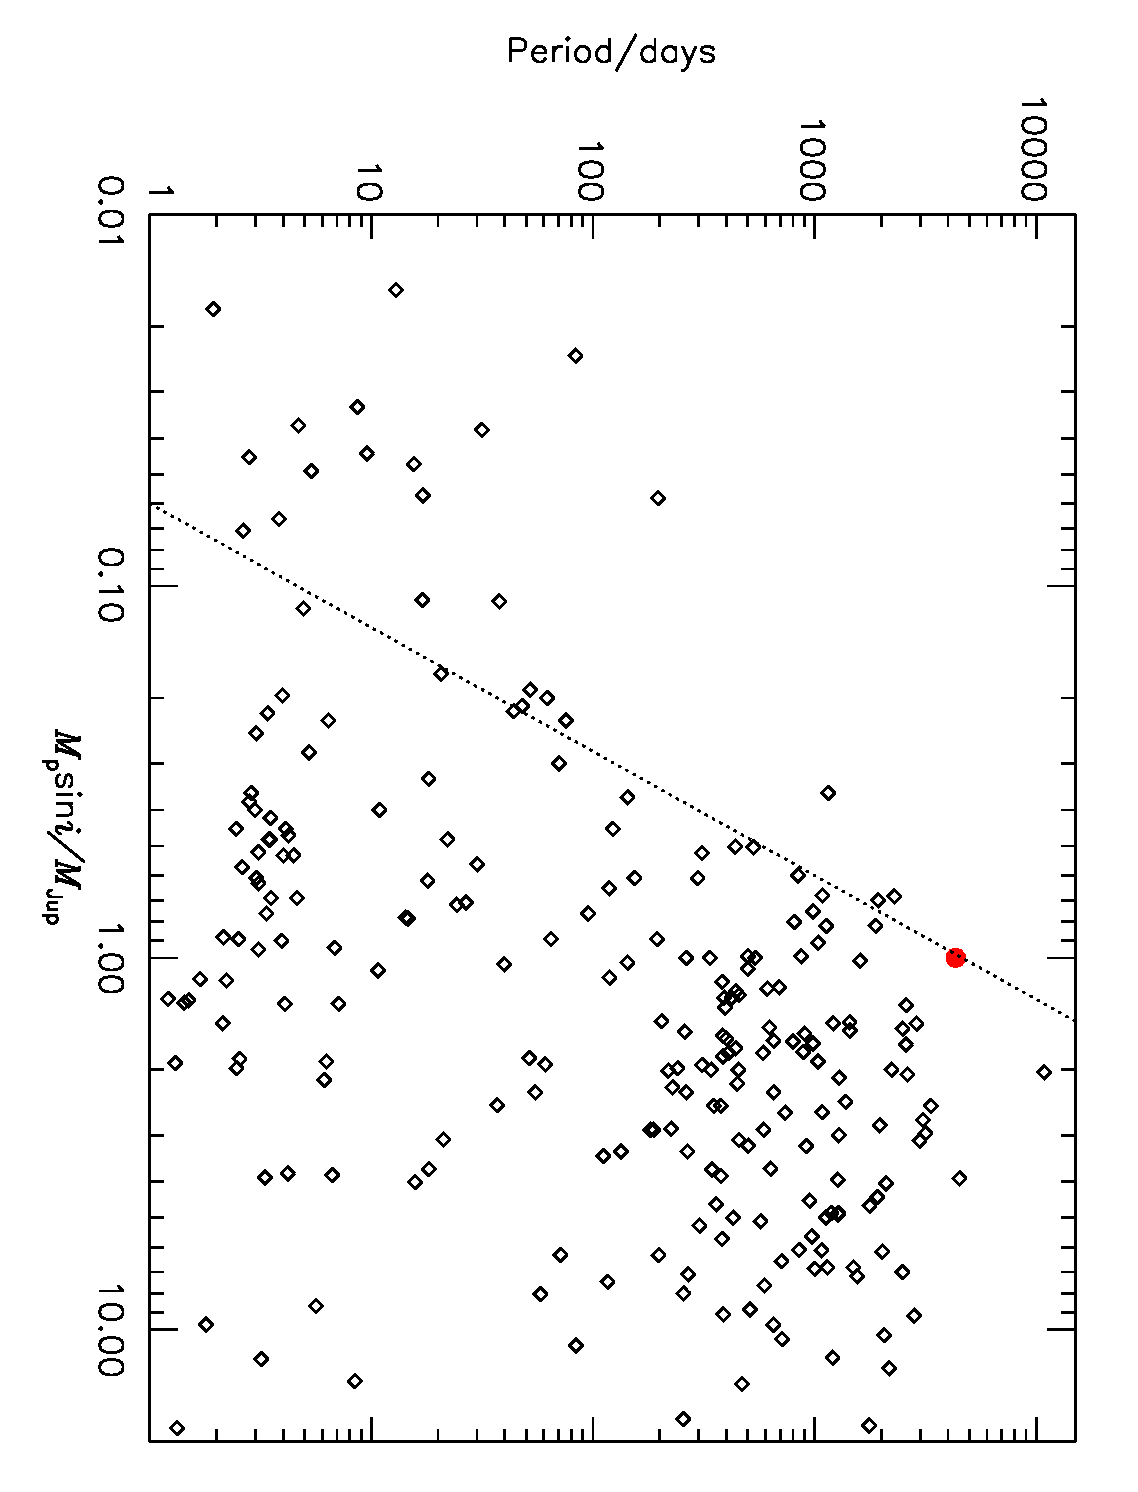
\includegraphics[angle=90,width=.90\textwidth]{1_rvplanets}
\caption[Orbital period distribution of the 232 known exoplanets]{%
Orbital period distribution of the 232 known exoplanets as a function of their minimum masses.
Jupiter is shown for comparison as a {\textit red, filled circle}.
Relatively few massive planets with short orbital periods have been found, despite the bias for such planets in the radial-velocity surveys.
An approximate detection threshold (defined as $K=4\sigma$, see text) is shown as a {\textit dotted line}.%
}\label{cha:intro:sec:methods:sub:rv:fig:rv}
\end{center}
\end{figure}

The enlarging catalog of planets from radial-velocity surveys of stars in the solar neighborhood facilitates studying the statistics of exoplanets.
For example, the frequency of planets can be estimated from the yield of these surveys, and is currently estimated at $\sim$5\% for planets of 0.5--8\,\mjup\ within 3\,AU \citep{Udry_Fischer_Queloz:PPV2007a}.
There is a correlation between the metallicity of stars and this frequency of planets around them (\citealp{Gonzalez:mnras:1997a, Fischer_Valenti:asp:2003a}; \citealp*{Santos_Israelian_Mayor:aa:2004a}; see \citealp{Gonzalez:pasp:2006a} for a review).
We can also see that known exoplanets have a wide range in orbital periods, as shown in figure~\ref{cha:intro:sec:methods:sub:rv:fig:rv}.
This figure also shows a distinct decreasing trend in the mass of the planet with the short orbital period (\citealp{Zucker_Mazeh:apjl:2002a}; \citealp*{Udry_Mayor_Santos:aa:2003a}), which may be related to the way in which these gas giants come to be located so close to their stars (see section~\ref{cha:intro:sec:form:subsec:birth}).
The lack of low mass planets at longer periods can be explained in terms of the detection threshold of radial-velocity surveys.
Planets can be detected if they induce a motion $K\gsim4\sigma$ in their star, where $\sigma$ is the uncertainty in each velocity measurement \citep*{Marcy_Cochran_Mayor:PPIV:2000a}.
Recent discoveries are made with uncertainties as low as $\sigma=1\ms$~\citep{Lovis_Mayor_Pepe:nat:2006a}.
The associated detection threshold, calculated using equation~\ref{cha:intro:sec:methods:sub:rv:eqn:mpsini} (assuming $\rstar=\rsun$), is shown in figure~\ref{cha:intro:sec:methods:sub:rv:fig:rv}.

\begin{figure}
\begin{center}
\centering
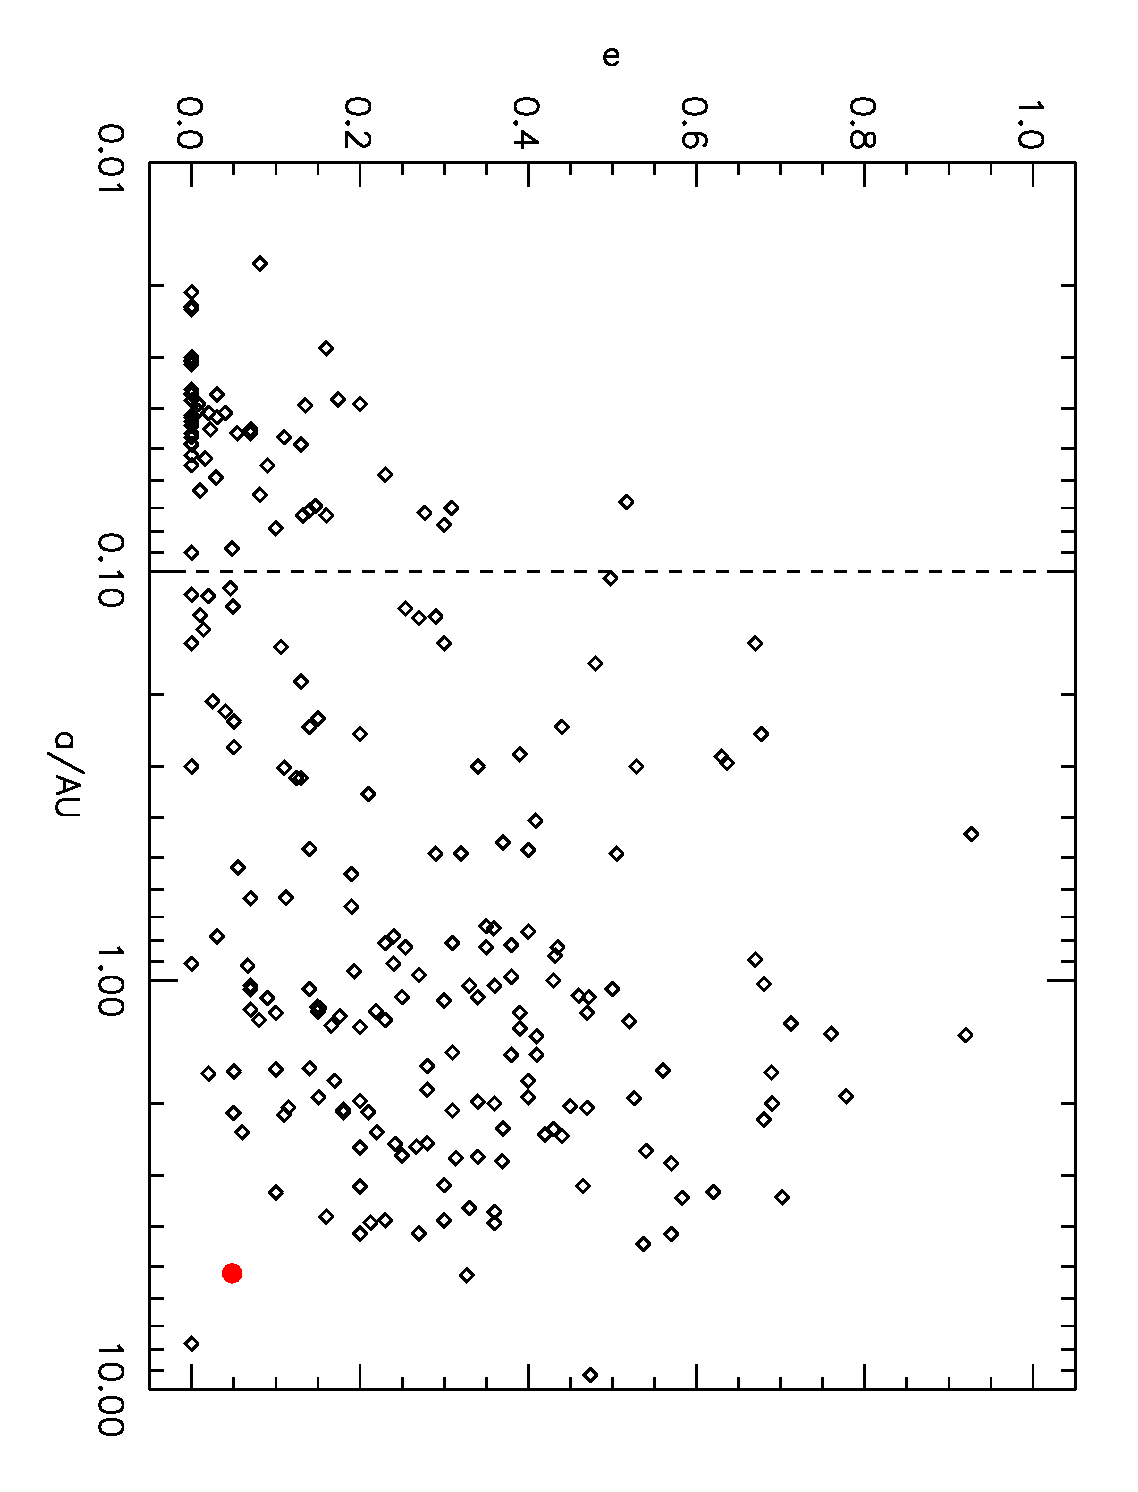
\includegraphics[angle=90,width=.90\textwidth]{1_rvplanetseccs}
\caption[Orbital eccentricity distribution of known exoplanets]{%
Orbital eccentricities of known exoplanets as a function of their orbital distance.
Jupiter is shown for comparison as a {\textit red, filled circle}.
Most of the hot Jupiters (those to the left of the {\textit dotted line}) have negligible eccentricity as expected from tidal circularization.%
}\label{cha:intro:sec:methods:sub:rv:fig:rve}
\end{center}
\end{figure}

Many of the known extrasolar gas giants have orbital periods much less than that of Jupiter (again, see figure~\ref{cha:intro:sec:methods:sub:rv:fig:rv}), much to the surprise of the early discoverers.
Extrasolar gas giants that orbit their stars within 0.1\,AU are known as {\textit hot Jupiters}, referring to the intense insolation experienced in a relative orbit well inside that of Mercury.
Tidal interactions (\citealp[see, e.g.,][]{Rasio_Ford:Science:1996a}) with the nearby star result in circular orbits for most of these close-in planets (see figure~\ref{cha:intro:sec:methods:sub:rv:fig:rve}).% chktex 10 chktex 9
Several planet searches such as this thesis work concentrate on these objects as they are both easier to find (due to their rapidly repeating signals) and fascinating to study (due to their extreme environment close to the star).
The proximity to the star also increases the probability that they will be observed to pass across the stellar disk.
The radial-velocity method achieves its full potential when combined with such transit observations, as this combined method allows a precise estimate of the mass and radius of the planet.

\subsection{Transits}\label{cha:intro:sec:methods:sub:trans}

For every system of gravitationally bound celestial objects, there is a probability that we will observe these objects passing in front of each other, eclipsing the light from the other.
In the case of a hot Jupiter with a radius $\rp$ in a circular orbit around a star of radius \rstar, this probability is given by:
\begin{eqnarray*}
P & = & \frac{\rp + \rstar}{a},\\
 & \simeq & \frac{\rstar}{a},\\
  & \simeq & 10\% \left( \frac{\rstar}{\rsun} \right) \left( \frac{a}{0.05 AU} \right)^{-1}, % chktex 3
\end{eqnarray*}
where 0.05\,AU is the median orbital distance for systems containing hot Jupiters \citep{Sackett:POSS:1999a}.
A planet in an 0.05\,AU orbit around a solar-sized star (with $P\sim10$\%) is therefore an ideal candidate to monitor for the transit of the planet across the star.

The passage of the planet across the stellar disk will block light from the star and reduce the flux by $\Delta F$.
For example, a transit of the Sun by Jupiter would block $\sim$1\% of the sunlight.
Assuming that \rstar\ can be determined from spectroscopy, the radius of the planet can then be calculated from:
\begin{eqnarray*}
r_{p} & = & {\rstar} \sqrt{\Delta F}.
\end{eqnarray*}
Such a transit would have a duration $D$ of:
\begin{eqnarray*}
D = \frac{P}{\pi} \arcsin{\left( \frac{\rstar}{a \sin{i}}
\sqrt{\left(1+\frac{\rp}{\rstar}\right)^2 - b^2} \right)}, % chktex 3
\end{eqnarray*}
where $b$ $(=a\cos{i}/\rstar)$ is the impact parameter \citep{Seager_Mallen-Ornelas:apj:2003a}.
For a Jupiter-sized planet that transits the equator of a solar-type star with a 4-day period, the transit duration $D\sim2.5$\,hours.

\begin{figure}
\begin{center}
\centering
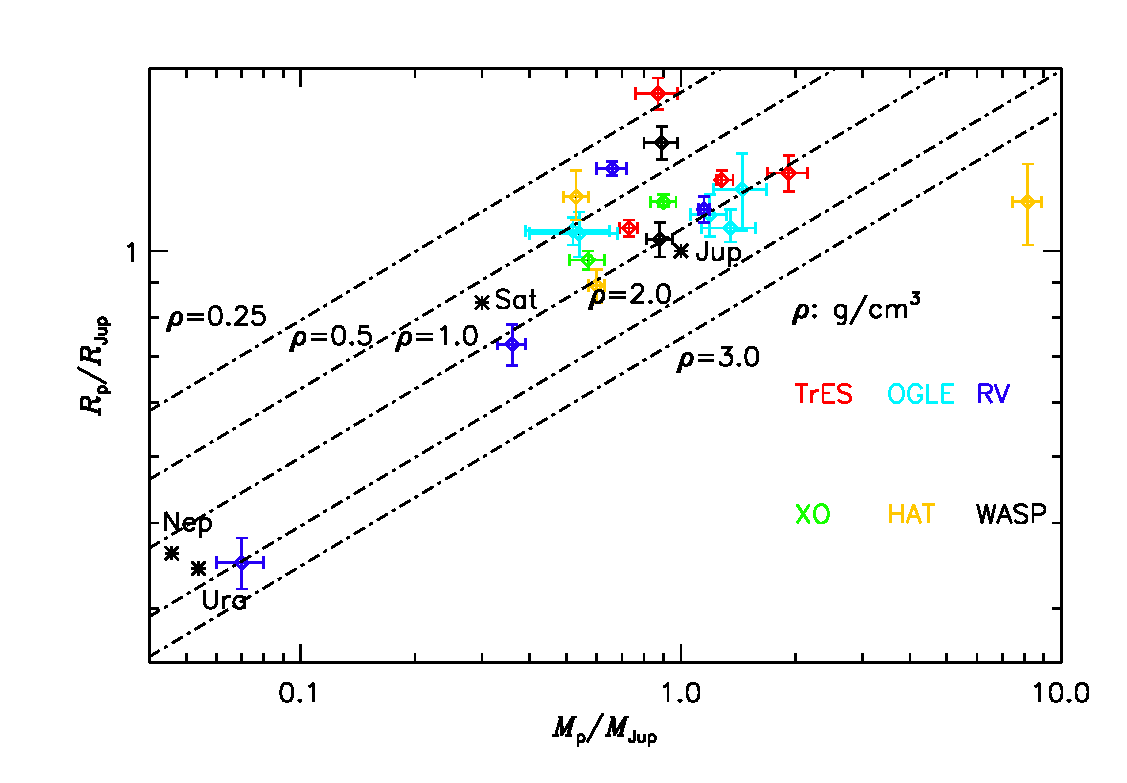
\includegraphics[width=.90\textwidth]{1_radii}\\
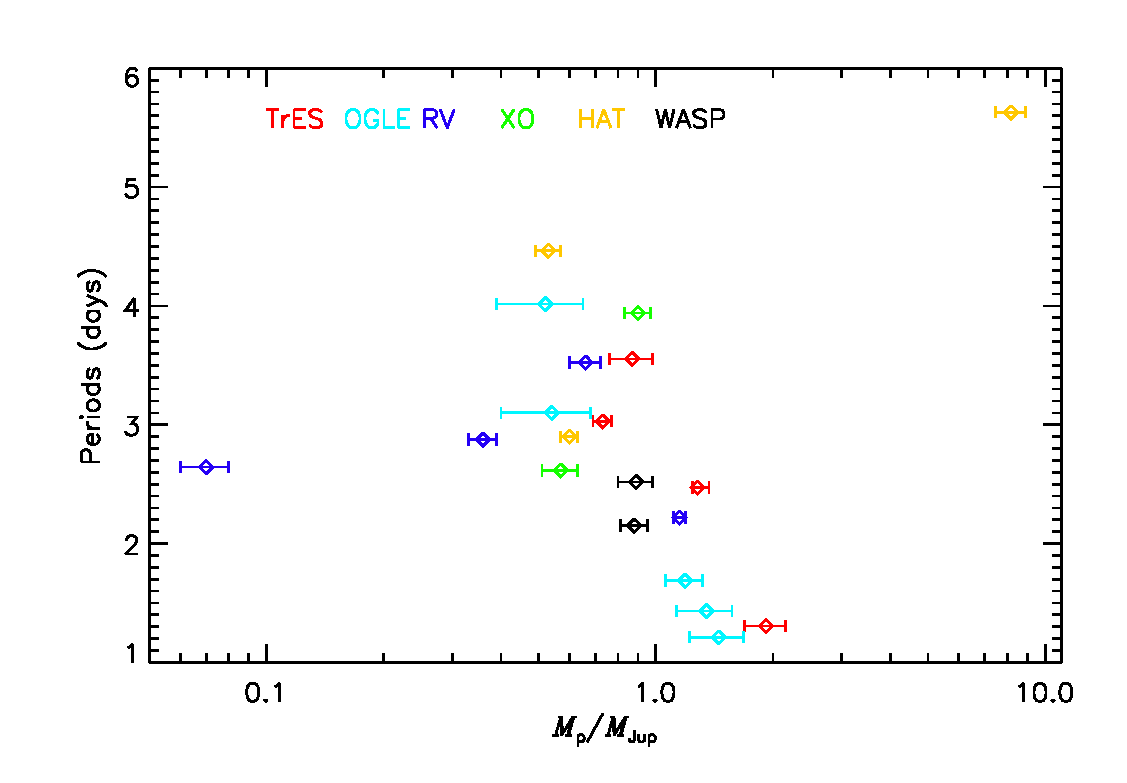
\includegraphics[width=.90\textwidth]{1_periods}\\
\caption[Mass-radius and mass-period relations for transiting planets]{%
Mass-radius ({\textit top}) and mass-period ({\textit bottom}) relations for the transiting planets known at the time of writing.
The {\textit dot-dashed lines} represent different densities.
There is a spread of radii for planets of the same mass, and reproducing the largest radii is still beyond current structural models.
There also appears to be a decreasing trend in mass with period in the {\textit bottom panel}.
In the $\sim$1--2-day period range, the planets all have $\mp \geq \mjup$.
This may indicate different formation mechanisms for these planetary systems than those at longer periods.
}\label{cha:intro:sec:methods:sub:trans:fig:tp}
\end{center}
\end{figure}

In order for a transit to occur, the orbital inclination must be close to $90\degr$, hence the minimum mass derived for a transiting planet using equation~\ref{cha:intro:sec:methods:sub:rv:eqn:mpsini} is a close approximation of the true planetary mass.
By combining observations of transits and radial-velocity variations, astronomers have obtained mass and radius precise estimates of 20 transiting exoplanets (at the time of writing; see figure~\ref{cha:intro:sec:methods:sub:trans:fig:tp}) with which to test structural models for these giant balls of gas.
(For reference, I have placed tables of the properties of these transiting systems in appendix~\ref{cha:prop}.)
The masses of the transiting planets are clustered around $1\,\mjup$.
However, the discovery of the least massive (\gjFTSb) and most massive (\hatptwob) transiting planets to date suggest that over time the mass distribution will resemble more that of the radial-velocity planets (see figure~\ref{cha:intro:sec:methods:sub:rv:fig:rv}).

Figure~\ref{cha:intro:sec:methods:sub:trans:fig:tp} also shows the variation in orbital period with mass.
Although results thus far are limited by small number statistics, it appears that the more massive transiting planets have shorter orbital periods, and every $\mp<1\,\mjup$ planet has an orbital period greater than 2\,days.
This trend, which is in the opposite direction to the corresponding trend for the known radial-velocity planets (see figure~\ref{cha:intro:sec:methods:sub:rv:fig:rv}), was first noted by \citet*{Mazeh_Zucker_Pont:mnras:2005a} and \citet*{Gaudi_Seager_Mallen-Ornelas:apj:2005a}.
If the trend continues to be observed as more transiting planets are discovered in the range of orbital periods 1--5\,days, it may indicate a different origin for the planets with $\sim$one-day periods, perhaps by tidal capture rather than inward migration \citep{Gaudi_Winn:apj:2007a}.

In contrast to the number of known eccentric radial-velocity planets at small orbital separations (see figure~\ref{cha:intro:sec:methods:sub:rv:fig:rve}), there are only two known transiting planets (\gjFTSb\ and \hatptwob) in this category.
Again, over time when more transiting systems are known, it is likely that this number will significantly increase.

As well as providing the most precise masses and radii known for extrasolar planets, nearby transiting planets present some other unique opportunities to study their nature:
\begin{enumerate}
\textitem\
Space-based telescopes offer the promise of exquisitely precise transit light curve with which to look for evidence of rings and satellites orbiting the gas giant \citep[see, e.g.,][]{Brown_Charbonneau_Gilliland:apj:2001a}.
\textitem\
Radial-velocity observations of the star during transit can measure the strength of the Rossiter-McLaughlin effect \citep{McLaughlin:apj:1924a,Rossiter:apj:1924a}, an apparent radial-velocity variation caused by the blocking of light from the differentially rotating star.
The strength of the variation indicates the misalignment of the orbital and rotation axes of the system.
\textitem\
We can also observe the starlight as it transmits through the planetary atmosphere during transit, and look for spectral features indicative of the chemical composition of the planet~\citep{Charbonneau_Brown_Noyes:apj:2002a, Vidal-Madjar_Lecavelier-des-Etangs_Desert:nat:2003a, Vidal-Madjar_Desert_Lecavelier-des-Etangs:apjl:2004a, Deming_Brown_Charbonneau:apj:2005a, Barman:apjl:2007a}.
\textitem\
The relative flux of a hot Jupiter to that of the star is greatest in the infrared.
Since a transiting system undergoes a secondary eclipse as well as a primary eclipse (the transit), we can estimate the strength of this emission by comparing the system flux before the secondary eclipse, and the flux during the secondary eclipse when the star blocks the planetary flux.
Infrared emission has already been observed from several transiting planets using \spi\ \citep[see, e.g.,][]{Charbonneau_Allen_Megeath:apj:2005a, Deming_Seager_Richardson:nat:2005a}, and recently the first spectra of exoplanets were obtained \citep{Richardson_Deming_Horning:Nature:2007a, Swain_Bouwman_Akeson:preprint:2007a, Grillmair_Charbonneau_Burrows:apjl:2007a}, as well as the first map of the emission variation across a planet \citep{Knutson_Charbonneau_Allen:nat:2007a}.
\end{enumerate}

\section[Formation, Structure, and Composition of Highly-Irradiated Gas Giants]
{Formation, Structure, and Composition of \\ Highly-Irradiated Gas Giants}\label{cha:intro:sec:form}

Transiting systems provide precise measurements of planetary masses and radii and facilitate the direct study of the orbital alignment and spectral features of the planet.
In this section, I will explain how these observations serve as important constraints for models of the initial formation, internal structure and atmospheric composition of these distant gas giants.
Before the discovery of these giants in such extreme environments, the only constraints of theoretical models were the solar system gas giants.
Models based on our own planetary system proved to be inadequate for hot Jupiters.

\subsection{The Birth of Giants}\label{cha:intro:sec:form:subsec:birth}

The canonical model for the formation of gas giants prior to the discovery of hot Jupiters nicely reproduced the giant planets of our solar system.
In this core accretion model \citep[see, e.g.,][]{Pollack:araa:1984a,Pollack_Hubickyj_Bodenheimer:icarus:1996a}, the gas giant begins as a protoplanetary core within a nebular disk and grows through collisions with other protoplanets and the accretion of gas from the surrounding disk.
When the core is massive enough, a period of runaway gas accretion occurs, and a giant planet is born.
This core formation relies on a suitable quantity of icy particles in the surroundings to form planetesimals.
With the discovery of \mbox{51\,Peg\,b} \citep{Mayor_Queloz:nat:1995a}, a giant planet close to its star and well inside the {\textit ice line} (the boundary beyond where most material is in solid, rather than gaseous, form), the validity of this theory was called into question: how could this planet have formed a solid core so close to the star?

The most likely explanation is that hot Jupiters like \mbox{51\,Peg\,b} formed outside the ice line (as did the solar system gas giants), and then moved or {\textit migrated} inward toward the star (\citealp{Goldreich_Tremaine:apj:1980a}; Lin, Bodenheimer, \& Richardson~\citeyear{Lin_Bodenheimer_Richardson:nat:1996a}; \citealp{Trilling_Benz_Guillot:apj:1998a}).
This migration is enabled by gravitational interactions between the planet and the disk.
Whether the migration is halted by some mechanism or the observed planet survived simply because the disk dissipated in time to prevent further migration is still unresolved.

\subsection{A Core or Not a Core, That is the Question}\label{cha:intro:sec:form:subsec:core}

An alternative formation model for gas giants was proposed by~\citet{Boss:sc:1997a}.
In his gravitational instability model, gas giants can be formed rapidly as collapsing instabilities in the nebula.
A consequence of this rapid formation is that the gas giant is thought not to have a substantial core, although some heavy elements may be accumulated through planetesimal bombardment.

The ability to measure the masses and radii of hot Jupiters allows us to test for the presence or absence of cores, and thus differentiate between the two models.
Models of gas giants that include a substantial core have a smaller radius for the planet, and this effect is larger for the less massive giants.
There is some evidence for core accretion in the observations of transiting planets.
\hdOFNb\ is a transiting hot Saturn whose radius is so small for its mass that a large core of approximately 70\,\mearth\ of heavy elements is implied by the models~\citep{Sato_Fischer_Henry:apj:2005a, Charbonneau_Winn_Latham:apj:2006a, Fortney_Saumon_Marley:apj:2006a}.

However, ever since the discovery of \hdTZNb, we have struggled to adapt these models to explain every extrasolar mass-radius relation.
We have now identified several transiting gas giants whose radii exceed our predictions for their masses;
the values for the remaining planets are in agreement with models either with or without a core \citep[see,][for a review]{Laughlin_Wolf_Vanmunster:apj:2005a, Charbonneau_Brown_Burrows:PPV:2007a}.

In order to explain these ``inflated'' planets, several additional energy sources were proposed that could slow the contraction of the planet after formation, and would result in a larger radius.
\citet*{Bodenheimer_Lin_Mardling:apj:2001a} and \citet*{Bodenheimer_Laughlin_Lin:apj:2003a} suggested the presence of an additional but unseen planet in the transiting system that would continuously pump the orbital eccentricity of the detected planet.
The tidal circularization of this nonzero eccentricity would produce the energy internal to the planet required to maintain the large radius.
\citet{Winn_Holman:apjl:2005a} proposed a similar tidal dissipation, this time of a nonzero obliquity of a planet in a Cassini state.
The explanation put forth by \citet{Guillot_Showman:aa:2002a} and \citet{Showman_Guillot:aa:2002a} was that some of the intense insolation creates atmospheric winds and thereby contributes thermal energy to the interior.
\citet{Burrows_Hubeny_Budaj:apj:2007a} explored the effect of substantially increased planetary metallicity on the opacity of the planetary atmosphere and suggested that the resultant increased opacity would act to slow the heat loss from and hence contraction of the planet.
\citet*{Burrows_Sudarsky_Hubbard:apj:2003a} and \citet{Baraffe_Chabrier_Barman:aa:2003a} pointed out an effect due to the difference between the observed planetary radius (corresponding to an optical depth of unity at some wavelength) and the theoretical radius (at the 1-bar level) that could account for 5\% of the discrepancy between the two.

However, no satisfying solution has been found to date.
The kinetic energy source of \citet{Guillot_Showman:aa:2002a} should apply to every hot Jupiter, yet \hdTZNb\ and \tresOne\ have similar masses but significantly different radii.
\citet{Deming_Seager_Richardson:nat:2005a} refuted the possibility that tidal damping of a nonzero eccentricity was an energy source for the inflated planet \hdTZNb\ by deriving a negligible eccentricity from observations of a secondary eclipse.
Also, \citet*{Fabrycky_Johnson_Goodman:apj:2007a} has rejected obliquity tides as not providing enough energy through dissipation to account for large radii of hot Jupiters.

\subsection{Extrasolar Atmospheres}\label{cha:intro:sec:form:subsec:atm}

Although giant planets consist mainly of gas, namely molecular hydrogen and helium, both the absorption rate of incident radiation, and the emission from (and hence cooling rate of) the planet is determined mostly by a thin outer layer of these gaseous molecules.
This thin layer is called the {\textit atmosphere} of the planet.
The composition of the atmosphere, and the gas giant itself, is expected to be roughly the composition of the nebula from which it formed, although substantially enriched due to bombardment of planetesimals.
The presence or absence of specific chemical species in the atmosphere is then dependent on the temperature and pressure gradients of the planet.
The metallicity of the atmosphere can be a significant effect.
The infrared color of \tresOne~\citep{Charbonneau_Allen_Megeath:apj:2005a} is too red when compared to model spectra and other planets, and \citet{Fortney_Marley_Lodders:apjl:2005a} explained this as due to a metallicity 3--5 times solar.

Once again, the extreme nature of the environment of hot Jupiters presents a new challenge to models of gas giants, this time of their atmospheres.
Jupiter has an effective temperature of 125\,K, has an intrinsic luminosity due to ongoing contraction roughly equal to its luminosity due to reradiated solar flux, and almost completely redistributes the thermal energy from this flux from the dayside to the night-side of the planet.
In contrast, hot Jupiters have equilibrium temperatures of up to 1500\,K.
Of their luminosity, 99.99\% is due to the re-radiation of the insolation \citep{Marley_Fortney_Seager:PPV:2007a}.
This intense radiation may result in hot substellar spots, and could cause day-night temperature differences of up to $\sim$500\,K, and winds of up to 2\,\kms~\citep{Showman_Guillot:aa:2002a}.
The efficiency of the redistribution of the heat from this spot may vary from planet to planet.

Due to the high effective temperatures, atmospheric models predict different dominant molecular absorbers in the spectra of the hot Jupiters than of the solar system giants.
At the visible wavelengths, Na and K produce strong absorption features, whereas in the infrared, H$_2$O, CO, CH$_4$, and CH$_3$ are all noticeable absorbers.
The exact planetary spectrum depends on the amount of insolation absorbed by the planet, the redistribution of the resultant thermal energy, and the presence or absence of high clouds of condensates.
Unlike the solar system giants for which we have direct estimates of the solar flux and of the chemical compositions, we can be certain only of the incident radiation onto these planets.
However, if we measure the amount of flux from the night-side of a transiting planet (during a transit) and from the day-side (during a secondary eclipse), we can deduce how much energy is being transported from the dayside, and hence measure the efficiency of this redistribution.

Understanding the atmospheric makeup of the hot Jupiters may provide us with an explanation for the inflated exoplanets, as the predictions for these radii are dependent on understanding the cooling rates of the planets.


\section{Thesis Motivation---Past and Present}\label{cha:intro:sec:motivation}

At the beginning of my thesis work, only one transiting planet, \hdTZNb, was known.
The radius of this planet was larger than could be explained by extrapolating models of solar system gas giants to account for intense insolation.
This made the discovery of additional transiting planets very important to allow determination of whether this planet was merely an anomaly.
Transit surveys also held the promise of being the most effective way to obtain precise planetary masses and radii to provide constraints for models.
In contrast to the radial-velocity surveys of individual stars, transit surveys monitor thousands of stars at a time for evidence of a planetary companion, although the expected frequency of detections was not well understood.
With the TrES team's discovery of \tresOne~\citep{Alonso_Brown_Torres:apjl:2004a}, wide-field surveys proved our ability to find transiting planets around stars bright enough to provide these desired precise constraints.
It was clear that my wide-field transit survey could make a substantial contribution even by discovering only one or two transiting planets.
By extending the coverage of the parameter space for exoplanets, I could hope to improve the understanding of the wide range of radii for planets of similar masses.
The bright stars that I would find as part of my survey would also be ideal targets for detailed studies of the atmosphere and neighboring objects with space-based telescopes.

The goals that motivate my thesis work still hold today, since the number of known transiting planets (19) is still quite low.
The planets found by TrES and other surveys continue to be much sought after, and quickly observed with the best instruments available to uncover the true nature of each planet.

\section{Thesis Outline}\label{cha:intro:sec:outline}

The goals of my thesis were to both detect and explore new transiting planets.
Much of my thesis work involved participation in the Trans-atlantic Exoplanet Survey (TrES), a network of three ten-centimeter optical telescopes used to search for nearby transiting planets.

For four years, I have operated and maintained the telescope Sleuth at Palomar Observatory, obtaining observations of TrES fields almost every night (weather permitting).
I have reduced these observations, and searched the resulting time series of field stars for transit signals.
For each transit candidate that I identified, it has been my responsibility to then coordinate follow-up spectroscopic observations, obtained by D.~Latham and collaborators, and follow-up photometric observations, obtained by me and several TrES collaborators.
I pursued my own follow-up photometry using Sherlock \citep{Kotredes_Charbonneau_Looper:2004a} or the Palomar 1.5-meter telescope \citep[see, e.g.,][for an example of the 1.5-meter photometry]{Holman_Winn_Latham:apj:2006a}, and performed modeling of this photometry to derive precise transit parameters.
Based on the results of each new set of observations, I removed false positives from my candidate list.

Twice during my thesis, I obtained high-dispersion observations of my most promising transit candidates with Keck/HIRES, aided by D.~Charbonneau, G.~Torres, and A.~Sozzetti, who performed the rapid data analysis needed to review the data while still at Keck.
The subsequent required blend analysis and photometric modeling of the three planets that I discovered were performed by G.~Torres and D.~Charbonneau, respectively.

Having discovered \tresTwo, I then turned my attention to analyzing the \spi\ observations of this planet, obtained by my collaborator J.~Harrington.
The theoretical interpretation of the data was carried out in collaboration with S.~Seager.

Most of the chapters in this thesis are based on material published during my time at Caltech.
I have presented them in a logical order, rather than ordered by publication date.

In chapter~\ref{cha:and0}, I outline how I obtained observations of 26,495 stars in a single field using Sleuth, and my analysis of the data.
I present six candidates that I identified from a transit search of the photometry.
I explore the methods used by the TrES team to reject astrophysical false positives, and explain how the six stars were culled from our candidate transiting system list.
In this chapter, I also demonstrate the advantages of a multisite network such as TrES for obtaining better phase coverage and confirming the reliability of these candidates.

Most transit surveys have obtained significant experience with these typical astrophysical false positives.
In chapter~\ref{cha:gsc}, I discuss an early example of a more insidious false positive, \gscOTE, that I identified as a candidate transiting planet.
This system proved to be a solitary star blended with an eclipsing binary.
The relative faintness of the binary prevented the detection of its radial-velocity signal.
Multicolor photometry revealed a color-dependent eclipse, indicative of the binary nature.
In this chapter, I go into more detail about how I produce light curves from Sleuth photometry and select transit candidates.

In chapter~\ref{cha:tres2}, I present the discovery in one of the Sleuth fields of a massive gas giant \tresTwo\ that was confirmed from the spectroscopic orbit derived from my observations with Keck/HIRES.\@
\tresTwo\ is the first transiting planet known to reside in the field of view of the upcoming NASA {\textit Kepler} mission that will search for new exoplanets.
Similarly, in chapter~\ref{cha:tres3}, I present \tresThree, another massive transiting planet from a Sleuth field, this time with a very-short orbital period.
This discovery has further cemented the hypothesis that the nearby exoplanets discovered by wide-field transit surveys and the more distant gas giants found by narrow-field transit surveys have the same intrinsic period distribution.
I have also included in appendix~\ref{cha:tres4} the discovery paper for \tresFour, the third planet found in a Sleuth field.
This planet has the largest radius and lowest density of the currently known transiting planets.

Although each newly discovered transiting planet automatically provides a new constraint for theoretical structural models for these Jovian planets, the nearby transiting planets also present promises of a more detailed exploration.
{\textit Spitzer} has been a leading source of new information about exoplanets, and in chapter~\ref{cha:spitzer}, I present my analysis of the first \spi/IRAC observations of \tresTwo, and determine a negligible orbital eccentricity for this hot Jupiter. There is no evidence of strong atmospheric absorption from these observations, but future analysis including additional \spi\ observations will be more conclusive.

Finally, I examine the yield of planets from this survey in comparison with predictions.
In chapter~\ref{cha:human}, I present initial results from a study of my ability to recover fake transit light curves injected into real data from a TrES field.
Rather than just concentrate on the recovery rate of the transit-search algorithm I employ, I explore the human element of identifying worthy planet candidates, and the resultant recovery rate of transit candidates.

The photometric data from Sleuth have also been of value in the study of eclipsing binaries. As this is not related to my thesis goals, I simply refer the reader to \citet{Creevey_Benedict_Brown:apjl:2005a} and Devor et al.~(2007, in preparation) as examples of this use of Sleuth data.% chktex 17


% chktex-file 44 chktex-file 15
\chapter[Outcome of Six Candidate Transiting Planets from a TrES Field in Andromeda]{Outcome of Six Candidate Transiting Planets from a TrES Field in Andromeda%
\protect\CFNB%
}\label{cha:and0}

\section*{Abstract}\label{cha:and0:sec:abs}
\addcontentsline{toc}{section}{Abstract}

Driven by the incomplete understanding of the formation of gas giant extrasolar planets and of their mass-radius relationship, several ground-based, wide-field photometric campaigns are searching the skies for new transiting extrasolar gas giants. As part of the Trans-atlantic Exoplanet Survey (TrES), in 2003/2004 we monitored approximately 30,000 stars ($9 .5\leq V \leq 15.5$) in a $5.7\degr\times5.7\degr$ field in Andromeda with three telescopes over five months. We identified six candidate transiting planets from the stellar light curves. From subsequent follow-up observations we rejected each of these as an astrophysical false positive, i.e., a stellar system containing an eclipsing binary, whose light curve mimics that of a Jupiter-sized planet transiting a Sun-like star. We discuss here the procedures followed by the TrES team to reject false positives from our list of candidate transiting hot Jupiters. We present these candidates as early examples of the various types of astrophysical false positives found in the TrES campaign, and discuss what we learned from the analysis.

\section{Finding a Needle in a Haystack}\label{cha:and0:sec:intro}

At the time of writing, there are 14 extrasolar planets for which we have measurements of both the planetary radius and mass (\citealp*[see][for a review]{Charbonneau_Brown_Burrows:PPV:2007a}; \citealt{McCullough_Stys_Valenti:apj:2006a}; \citealt{ODonovan_Charbonneau_Mandushev:apjl:2006a}, see chapter~\ref{cha:tres2}; \citealt{Bakos_Noyes_Kovacs:apj:2007a, Collier-Cameron_Bouchy_Hebrard:MNRAS:2007a}). These gas giants have been observed to transit their parent stars and have supplied new opportunities to study Jupiter-sized exoplanets, in particular their formation and structure. Studies of the visible and infrared atmospheric spectra are possible for the nine nearby ($d<300$\,pc) transiting planets \citep{Charbonneau_Brown_Noyes:apj:2002a, Vidal-Madjar_Lecavelier-des-Etangs_Desert:nat:2003a, Deming_Brown_Charbonneau:apj:2005a, Deming_Seager_Richardson:nat:2005a, Charbonneau_Allen_Megeath:apj:2005a}.
The incident flux from the close-by (\mbox{$\lsim0.05\,\mathrm{AU}$}) star on each of these ``hot Jupiters" results in an inflated planetary radius. Current theoretical models that include this stellar insolation can account for the radii of only five of these nine nearby planets. \hdTZNb\ \citep{Charbonneau_Brown_Latham:apjl:2000a, Henry_Marcy_Butler:apj:2000a}, \tresTwo\ (\citealp{ODonovan_Charbonneau_Mandushev:apjl:2006a}, see chapter~\ref{cha:tres2}), \hatponeb\ \citep{Bakos_Noyes_Kovacs:apj:2007a}, and \wasponeb\ \citep{Collier-Cameron_Bouchy_Hebrard:MNRAS:2007a} have radii larger than predicted (\citealp[see][]{Laughlin_Wolf_Vanmunster:apj:2005a} and Charbonneau et al., \citeyear{Charbonneau_Brown_Burrows:PPV:2007a} for reviews of the current structural models for insolated hot Jupiters).
The sparse sampling and limited understanding of the mass-radius parameter space for extrasolar planets continue to motivate the search for new transiting planets. There are several small-aperture wide-field surveys targeting these objects, such as the Berlin Exoplanet Search Telescope (BEST; \citealt{Rauer_Eisloffel_Erikson:pasp:2004a}), the Hungarian Automated Telescope (HAT) network \citep{Bakos_Lazar_Papp:pasp:2002a, Bakos_Noyes_Kovacs:pasp:2004a}, the Kilodegree Extremely Little Telescope (KELT; \citealt*{Pepper_Gould_Depoy:AIP:2004a}), the Super Wide Angle Search for Planets (SuperWASP; \citealt{Street_Pollaco_Fitzsimmons:ASP:2003a}), Vulcan \citep{Borucki_Caldwell_Koch:pasp:2001a}, and XO \citep{McCullough_Stys_Valenti:pasp:2005a}, as well as deeper surveys like the Optical Gravitational Lensing Experiment (OGLE-III; \citealt{Udalski_Paczynski_Zebrun:acta:2002a}) that is probing the Galactic disk.

We are conducting a transit campaign, the {Trans-atlantic Exoplanet Survey}%
\footnote{See \url{http://www.astro.caltech.edu/\~ftod/tres/}\ .}%
\ (TrES), using a network of three ten-centimeter telescopes with a wide longitudinal coverage:
{Sleuth}%
\footnotemark[\value{footnote}]%
\ (located at Palomar Observatory, California; \citealt{ODonovan_Charbonneau_Kotredes:AIP:2004a}), the Planet Search Survey Telescope (PSST; Lowell Observatory, Arizona; \citealt{Dunham_Mandushev_Taylor:pasp:2004a}),
and the STellar Astrophysics and Research on Exoplanets%
\footnote{See \url{http://www.hao.ucar.edu/public/research/stare/stare.html}\ .}%
\ telescope ({STARE}; on the isle of Tenerife, Spain; \citealt{Alonso_Deeg_Brown:an:2004a}). Over several months the telescopes monitor a $5.7\degr \times 5.7\degr$ field of view containing thousands of nearby bright stars ($9.5\leq V \leq 15.5$), and we examine the light curves of stars with $V\leq14.0$ for repeating eclipses with the short-period, small-amplitude signature of a transiting hot Jupiter. We have discovered two transiting planets so far: \tresOne\ \citep{Alonso_Brown_Torres:apjl:2004a} and \tresTwo\ (\citealp{ODonovan_Charbonneau_Mandushev:apjl:2006a}, see chapter~\ref{cha:tres2}). In order to find these two transiting planets we have processed tens of candidates with light curves similar to that of a Sun-like star transited by a Jupiter-sized planet. For a typical TrES field at a Galactic latitude of $b\sim15\degr$, we find $\sim$10 candidate transiting planets (\citealp[see, e.g.,][]{Dunham_Mandushev_Taylor:pasp:2004a}). We expect few of these to be true transiting planets, and the remainder to be examples of the various types of astrophysical systems whose light curves can be mistaken for that of a transiting planet (\citealp[see, e.g.,][]{Brown:apjl:2003a, Charbonneau_Brown_Dunham:AIP:2004a}). These are: \\
\indent (i) low-mass dwarfs eclipsing high-mass dwarfs, \\
(ii) giant+dwarf eclipsing binaries, and \\
(iii) grazing incidence main-sequence eclipsing binaries, \\
with eclipse depths similar to the $\sim$1\% transit depth of a hot Jupiter, and \\
(iv) blends, where a faint eclipsing binary and a bright star coincide on the sky or are physically associated, mixing their light, \\
with the observed eclipse depth reduced to that of a transiting planet.
We also encounter occasional photometric false positives, where the transit event is caused by instrumental error, rather than a true reduction in flux from the candidate. \citet{Brown:apjl:2003a} estimates the relative frequency of these astrophysical false positives. For a STARE field in Cygnus, he predicts that from every 25,000 stars observed with sufficient photometric precision to detect a transit, one can expect to identify one star with a transiting planetary companion. However, for this field near the Galactic plane ($b\sim3\degr$), the number of impostor systems identified as candidate planets will outnumber the true detections by an order of magnitude. (The yield of eclipsing systems from such transit surveys depends on the eclipse visibility, which is the fraction of such systems with a given orbital period for which a sufficient number of eclipses could be observed for the system to be detected.
This visibility varies with weather conditions during the observations and the longitudinal coverage of the telescopes used.)
Of the false positives, approximately half are predicted to be eclipsing binaries and half to be blends.

A careful examination of the light curve of a transit candidate may reveal evidence as to the nature of the transiting companion. Seager \& Mallen-Ornelas~(\citeyear{Seager_Mallen-Ornelas:apj:2003a}) present an analytic derivation of the system parameters that can be used to rule out obvious stellar systems. If the light curve demonstrates ellipsoidal variability, this indicates the gravitational influence of a stellar companion \citep{Drake:apj:2003a, Sirko_Paczynski:apj:2003a}. These tests have been used to great effect on the numerous candidates (177 to date) from the OGLE deep-field survey \citep{Drake:apj:2003a, Sirko_Paczynski:apj:2003a, Pont_Bouchy_Melo:aa:2005a, Bouchy_Pont_Melo:aa:2005a}, and candidates from wide-field surveys (\citealp[see, e.g.,][]{Hidas_Ashley_Webb:mnras:2005a, Christian_Pollacco_Skillen:mnras:2006a}).

The initial scientific payoff from each new transiting hot Jupiter comes when an accurate planetary mass and radius have been determined, which can then be used to test models of planetary structure and formation. These determinations require a high-quality light curve together with a spectroscopic orbit for the host star. For each TrES target field we follow a procedure of careful examination of each candidate, with follow-up photometry and spectroscopy to eliminate the majority of false positive detections and obtain a high-quality light curve before committing to the final series of observations with ten-meter class telescopes to determine the radial velocity orbit of the candidate planet. This procedure is similar to those discussed by \citet{Charbonneau_Brown_Dunham:AIP:2004a} and \citet{Hidas_Ashley_Webb:mnras:2005a}. Here we discuss our follow-up strategy (section~\ref{cha:and0:sec:elim}) and present the step-by-step results of this procedure for a field in Andromeda, one of the first fields observed by all three nodes of the TrES network. We describe the TrES network observations in section~\ref{cha:and0:sec:obs} and outline the initial identification of six candidates from the stellar light curves in section~\ref{cha:and0:sec:search}. Based on our follow-up observations of these candidates (section~\ref{cha:and0:sec:followup}), we were able to conclude that each was an astrophysical false positive (section~\ref{cha:and0:sec:reject}).

\section[Follow-up Observations of Planetary Candidates: A Review]{Follow-up Observations of Planetary \\ Candidates: A Review}\label{cha:and0:sec:elim}

The light curves from small wide-angle telescopes are not of sufficient quality to derive an accurate radius ratio for the purpose of both false positive rejection and planetary modeling, so high-quality follow-up photometric observations with a larger telescope are needed. Recent experience suggests that a photometric accuracy better than 1\,mmag with a time resolution better than one minute can be achieved with a meter-class telescope at a good site, and such observations can
deliver radius values good to a few percent and transit times good to 0.2\,minutes \citep{Holman_Winn_Latham:apj:2006a, Holman_Winn_Fuentes:apj:2007a}. For smaller telescopes, scintillation can limit the photometric precision at this cadence \citep{Young:aj:1967a, Dravins_Lindegren_Mezey:pasp:1998a}.

The wide-angle surveys by necessity have broad images, typically with FWHM values of $20\arcsec$. Thus, there is a significant probability of a chance alignment between a relatively bright star and a fainter eclipsing binary that just happens to be nearby on the sky. Photometric observations with high spatial resolution on a larger telescope can be used to sort out such cases by resolving the eclipsing binary (\citealp[see, e.g.,][]{Charbonneau_Brown_Dunham:AIP:2004a}). In some instances these systems can also be detected using the wide-angle discovery data, by showing that there is differential image motion during the transit events, even though the eclipsing binary is unresolved. Photometry can also be successful in identifying a triple. If the color of the eclipsing binary is different enough from that of the third star, high-quality multicolor light curves will reveal the color-dependent eclipse depths indicative of such a system (\citealp[see, e.g.,][]{Tingley:aa:2004a}; \citealp{ODonovan_Charbonneau_Torres:apj:2006a}, see chapter~\ref{cha:gsc}).

A practical problem for this follow-up photometry is that the transiting-planet candidates do not emerge from the wide-angle surveys until late in the observing season, when the observability of the candidates do not permit full coverage of a transit event. With only partial coverage of an event it is difficult to remove systematic drifts across the event, reducing the accuracy of the derived transit depth. Furthermore, full coverage of a transit is important for deriving very accurate transit timings. Without accurate ephemerides, the error in the predicted transit times during the next observing season may be too large to facilitate follow-up photometric observations. The typical duty cycle for a transit is a few hours over a period of a few days, i.e., a few percent. Therefore, if the follow-up photometry does not confirm a transit, the interpretation is ambiguous. The ephemeris may have been too inaccurate, or perhaps the original transit event was a photometric false detection.

One approach to recovering transits and providing an updated ephemeris for high-quality photometric observations with a larger telescope is to monitor candidates with intermediate sized telescopes, such as TopHAT in the case of the HAT survey \citep{Bakos_Noyes_Kovacs:pasp:2004a}, Sherlock \citep{Kotredes_Charbonneau_Looper:2004a} in the case of TrES, or teams of amateur telescopes \citep{McCullough_Stys_Valenti:apj:2006a} in the case of XO.

A second approach to confirming that a candidate is actually a planet is to obtain very precise radial velocities to see whether the host star undergoes a small reflex motion as expected for a planetary companion. This approach has the advantage that the velocity of the host star varies continuously throughout the orbit, so the observations can be made at any time with only modest attention to the phasing compared to the photometric period.  The ephemeris can then be updated using the velocities, to provide reliable transit predictions for the follow-up photometry. A second advantage is that a spectroscopic orbit is needed anyway to derive the mass of any candidate that proves to be a planet.  The big disadvantage of this approach is that a velocity precision on the order of $10\,\mathrm{m\,s^{-1}}$ is needed, which requires access to a large telescope with an appropriate spectrograph.

For the follow-up of transiting-planet candidates identified by TrES, we have adopted a strategy designed to eliminate the vast majority of astrophysical false positives with an initial spectroscopic reconnaissance using the Harvard--Smithsonian Center for Astrophysics (CfA) Digital Speedometers \citep{Latham:ASP:1992a} on the 1.5-meter Wyeth Reflector at the Oak Ridge Observatory in Harvard, Massachusetts and on the 1.5-meter Tillinghast Reflector at the F.~L.~Whipple Observatory (FLWO) on Mount Hopkins, Arizona. We aim to observe candidates spectroscopically during the same season as the discovery photometry. These instruments provide radial velocities good to better than $1\,\mathrm{km\,s^{-1}}$ for stars later than spectral type A that are not rotating too rapidly, and thus can detect motion due to stellar companions with just two or three exposures (\citealp[see, e.g.,][]{Latham:ASP:2003a, Charbonneau_Brown_Dunham:AIP:2004a}). Thus even if the follow-up is not performed until the target field is almost setting, we can still reject some candidates spectroscopically, even when photometric follow-up is not useful. For periods of a few days the limiting value for the mass detectable with these instruments is about 5--10\,$M_{\mathrm Jup}$.

The spectra obtained with these instruments also allow us to characterize the host star. We use a library of synthetic spectra to derive values for the effective temperature and surface gravity (assuming solar metallicity) and also the line broadening.  In our experience, rotational broadening of more than $10\,\mathrm{km\,s^{-1}}$ is a strong hint that the companion is a star, with enough tidal torque to synchronize the rotation of the host star with the orbital motion. Although the gravity determination is relatively crude, with an uncertainty of perhaps 0.5 in $\log{g}$, it is still very useful for identifying those host stars that are clearly giants with $\log{g} \leq 3.0$.  We presume that these stars must be the third member of a system that includes a main-sequence eclipsing binary, either a physical triple or a chance alignment, and we make no further follow-up observations. Our spectroscopic classification of the host star is a first step toward estimating the stellar mass and radius. These estimates, in turn, may be combined with the observed radial velocity variation and light curve to yield estimates of the mass and radius of the companion.

Although the use of follow-up spectroscopy has the scheduling advantages outlined above, the combination of both spectroscopy and photometry may be needed in the case of a blend. Such a candidate might pass our spectroscopic test as a solitary star with constant radial velocity, if the eclipsing binary of the triple is faint enough relative to the primary star (as was the case for \gscOTE; \citealt{ODonovan_Charbonneau_Torres:apj:2006a}, see chapter~\ref{cha:gsc}).

High-precision, high-signal-to-noise spectroscopic observations of the few remaining candidate transiting planets should reveal the mass (and hence true nature) of the transiting companion. However, even after a spectroscopic orbit implying a planetary companion has been derived, care must be taken to show that the velocity shifts are not due to blending with the lines of an eclipsing binary in a triple system (\citealp[e.g.,][]{Mandushev_Torres_Latham:apj:2005a}). It may be hard to see the lines of the eclipsing binary, partly because the eclipsing binary can be quite a bit fainter than the bright third star, and partly because its lines are likely to be much broader due to synchronized rotation.  In some cases it may be possible to extract the velocity of one or both the stars in the eclipsing binary using a technique such as TODCOR \citep{Mandushev_Torres_Latham:apj:2005a}. Combining modeling of the photometric light curve and information from the spectroscopic pseudo orbit for the system can help guide the search for the eclipsing binary lines.  Even if the lines of the eclipsing binary cannot be resolved, a bisector analysis of the lines of the third star may reveal subtle shifts that indicate a binary companion.

Follow-up observations with one-meter class telescopes both remove astrophysical false positives from consideration and prepare for the eventual modeling of newly discovered transiting planets. In the case of our field in Andromeda, our follow-up ruled out all of our planet candidates, and provided us with a variety of false positives to study.

\section[Initial Observations of a Field in Andromeda]{Initial Observations of a Field \\ in Andromeda with the TrES Network}\label{cha:and0:sec:obs}

\begin{figure}
\begin{center}
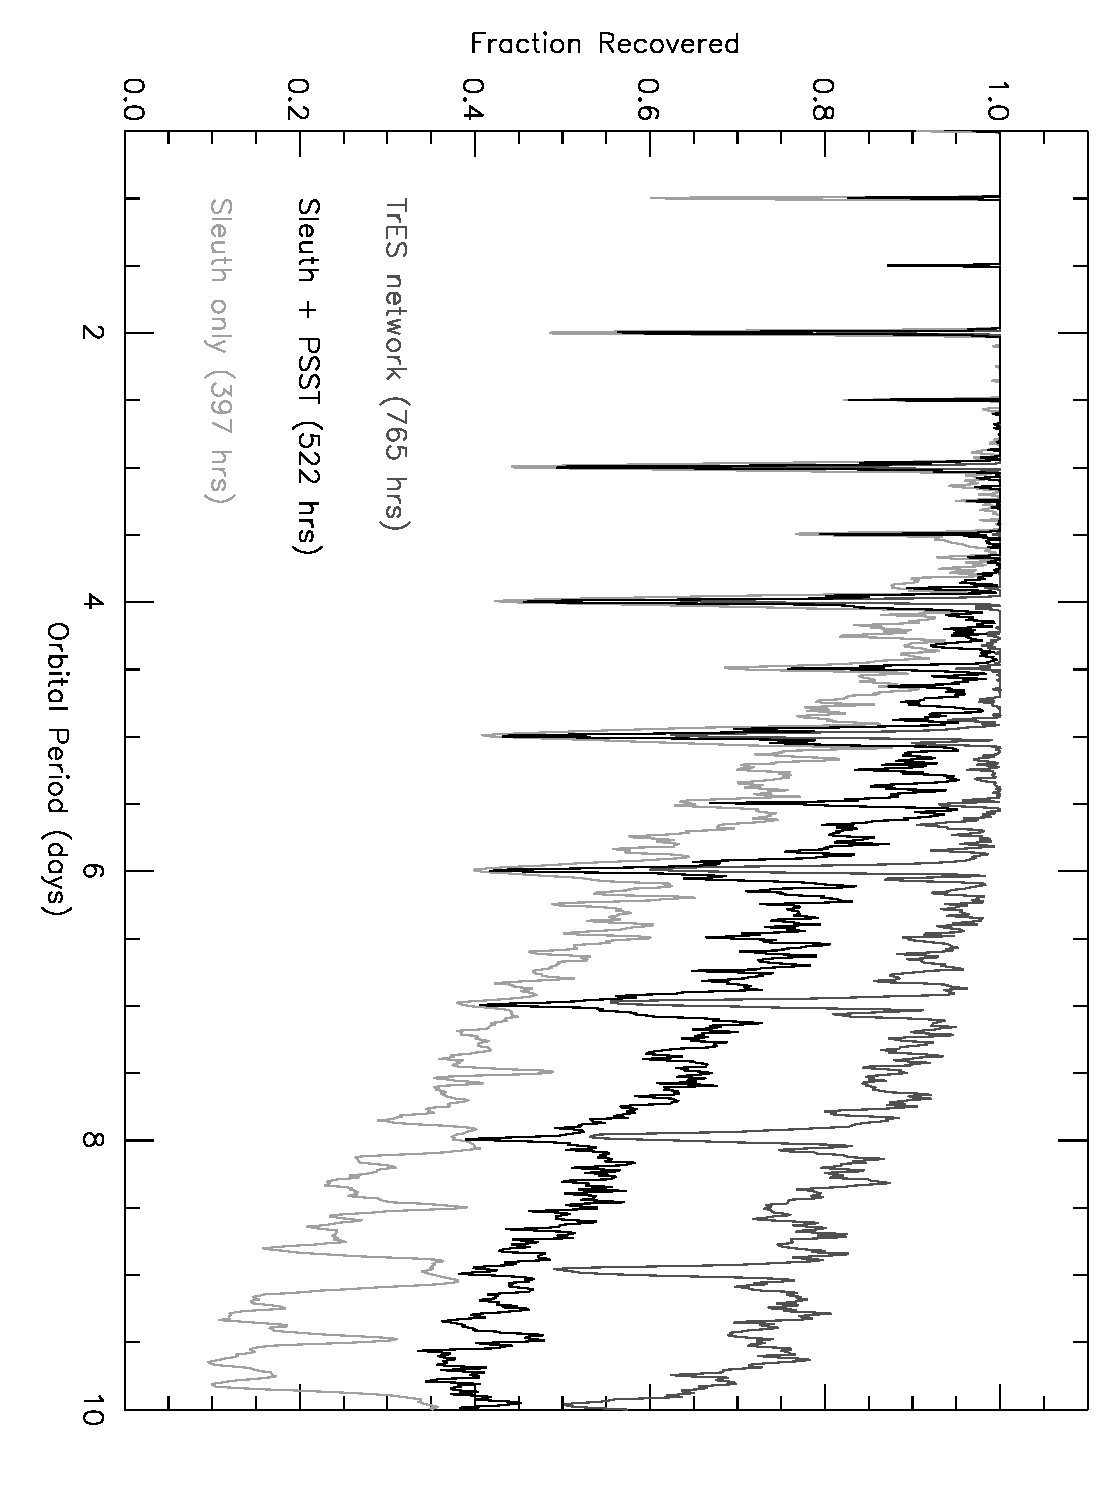
\includegraphics[angle=90, width=0.95\textwidth]{2_f1}
\caption[Fraction of potential transit signals identifiable from And0 data]{Transit visibility plot for the Andromeda field calculated from observations made using Sleuth alone (\textit{light gray}), Sleuth and the PSST (\textit{black}), and all three TrES telescopes (\textit{dark gray}). The fraction of transit signals with a given period identifiable from the data is plotted, assuming a requirement of observing three distinct transit events, with coverage of at least half of each individual event. About 80\% of transit events with periods less than 8 days should be recoverable from the TrES observations, whereas the Sleuth observations alone provide 80\% coverage only up to five-day periods.}\label{cha:and0:fig:vis}
\end{center}
\end{figure}

In 2003~August, we selected a new field centered on the guide star \mbox{HD\,6811} ($\alpha = 01^{\mathrm h} 09^{\mathrm m} 30.13^{\mathrm s}$, $\delta = +47\degr 14\arcmin 30.5\arcsec$ J2000.0).
We designated this target field as And0, the first TrES field in Andromeda.
We observed this field with each of the TrES telescopes.
Although the TrES network usually observes concurrently, in this case weather disrupted our observations.
Sleuth monitored the field through an SDSS $r$ filter for 42 clear nights between UT 2003 August~27 and October~24.
STARE began its observations with a Johnson $R$ filter on UT 2003 September~17 and observed And0 until UT 2004 January~13 during 23 photometric nights.
PSST went to this field on UT 2003 November~14 and collected Johnson $R$ observations until 2004~January~11, obtaining 19 clear nights.
We estimate our recovery rate for transit events should be 100\% for orbital periods $P<6$ days, declining to 70\% for $P=10$ days (see figure~\ref{cha:and0:fig:vis}), where here our recovery criterion is the observation of at least half the transit from three distinct transit events.
We note that this recovery rate is a necessary but not sufficient criterion to detect transiting planets, since it neglects the signal-to-noise ratio and the detrimental effect of non-Gaussian noise on it (\citealp*[see, e.g.,][]{Gaudi_Seager_Mallen-Ornelas:apj:2005a}; \citealp{Gaudi:apjl:2005a}; \citealp*{Pont_Zucker_Queloz:mnras:2006a}; \citealp{Smith_Collier-Cameron_Christian:mnras:2006a, Gaudi_Winn:apj:2007a}).
We used an integration time of 90\,s for our exposures.
During dark time, we took multicolor photometry (SDSS $g$, $i$, and $z$ for Sleuth and Johnson $B$ and $V$ for PSST and STARE) for stellar color estimates.

\section[Searching for Transit Candidates in Andromeda]{Searching for Transit Candidates \\ in Andromeda}\label{cha:and0:sec:search}

We have previously described in detail our analysis of TrES data sets in \citet{Dunham_Mandushev_Taylor:pasp:2004a} and \citeauthor{ODonovan_Charbonneau_Torres:apj:2006a}~(\citeyear{ODonovan_Charbonneau_Torres:apj:2006a}, see chapter~\ref{cha:gsc} for more details).
 We summarize here the analysis for this field. We used standard IRAF%
\footnote{IRAF is distributed by the National Optical Astronomy
  Observatories, which are operated by the Association of Universities
  for Research in Astronomy Inc. under cooperative agreement with
  the National Science Foundation.}%
\ \citep{Tody:1993a} tasks or customized IDL routines to calibrate the images from the three telescopes. For each telescope, we derived a standard list of stars visible in the images from this telescope and computed the corresponding equatorial  coordinates using the Tycho-2 Catalog \citep{Hog_Fabricius_Makarov:aa:2000a}. We applied differential image analysis (DIA) to each of the separate photometric data sets from the three telescopes using the following pipeline based in part on \citet{Alard:aas:2000a}. For each star in our standard star lists, we obtained a time series of differential magnitudes with reference to a master image. We produced this master image by combining 20, 18, and 15 of the best-quality interpolated images in our Sleuth, PSST, and STARE data sets, respectively. Since small-aperture, wide-field surveys such as TrES often suffer from systematics (caused, for example, by variable atmospheric extinction), we decorrelated the time series of our field stars.

\begin{deluxetable}{lccc}
\tablewidth{0pt}
\tablecaption{TrES labels, 2MASS and GSC designations, and approximate $V$ magnitudes for And0 candidate transiting systems
\label{cha:and0:tab:names}}
\tablehead{ \colhead{Candidate} & \colhead{2MASS \tablenotemark{a}}  &  \colhead{GSC \tablenotemark{b}} & \colhead{$V$}}

\startdata
\tOne    & 01083088+4938442 & 03272-00845 & 11.4 \\
\tTwo    & 00531053+4717320 & 03266-00642 & 11.6 \\
\tThree & {01023745+4808421} & {03267-01450} & 12.0 \\
\tFour   & {01180059+4927124} & {03272-00540} & 12.2 \\
\tFive    & {00545421+4805505} & {03266-00119} & 12.7\\
\tSix      & {00595445+4902030} & {03271-01102} & 12.7
\enddata
\tablenotetext{a}{Designations from 2MASS Catalog \citep{Cutri_Skrutskie_van-Dyk:2003a}, giving the coordinates of the sources in the form \mbox{hhmmss.ss+ddmmss.s} J2000.0.}
\tablenotetext{b}{GSC Catalog \citep{Lasker_Sturch_McLean:aj:1990a}.}
\end{deluxetable}

\begin{deluxetable}{lccccccl}
\rotate
\tablewidth{0pt}
\tablecaption{Transit properties for the six TrES And0 candidates\label{cha:and0:tab:transits}}

\tablehead{
\colhead{Candidate} & \colhead{SDE} & \colhead{Depth}  & \colhead{Period}  & \colhead{Duration} & \colhead{$N$  \tablenotemark{a}} & \colhead{Telescope(s) \tablenotemark{b}}& \colhead{True Nature} \\
\colhead{} & \colhead{} & \colhead{(mag)} & \colhead{(days)} & \colhead{(hr)} & \colhead{} & \colhead{} & \colhead{}
}

\startdata
\tOne & 19.3 & 0.005 & 1.1198 & 1.6  &  7 &  S,T & Eclipsing binary \\
\tTwo & \phn \phn 9.6 \tablenotemark{c} & 0.009 & 4.6619 & 3.4 &  2 & S & A-type star  \\
\tThree & 13.8 &  0.017 & 4.7399 & 3.4 & 5 & S,P,T & Eclipsing binary \\
\tFour & 21.5 & 0.019 & 3.0691 & 2.2 & 3 & S,P & Eclipsing binary \\
\tFive & 12.7 & 0.007 & 2.6540 & 3.2 & 7 & S,P & Blend \\
\tSix & 18.2 & 0.007 & 2.3556 & 3.4 & 7 & S,P,T & Rapidly rotating A-type star
\enddata
\tablenotetext{a}{The number of distinct transits observed in the TrES data set.}
\tablenotetext{b}{TrES telescopes that detected transits of this candidate, where S is Sleuth, P is PSST, and T is STARE.}
\tablenotetext{c}{Here the SDE is based on the Sleuth data set rather than the TrES combined observations.}
\end{deluxetable}

\begin{figure}
\begin{center}
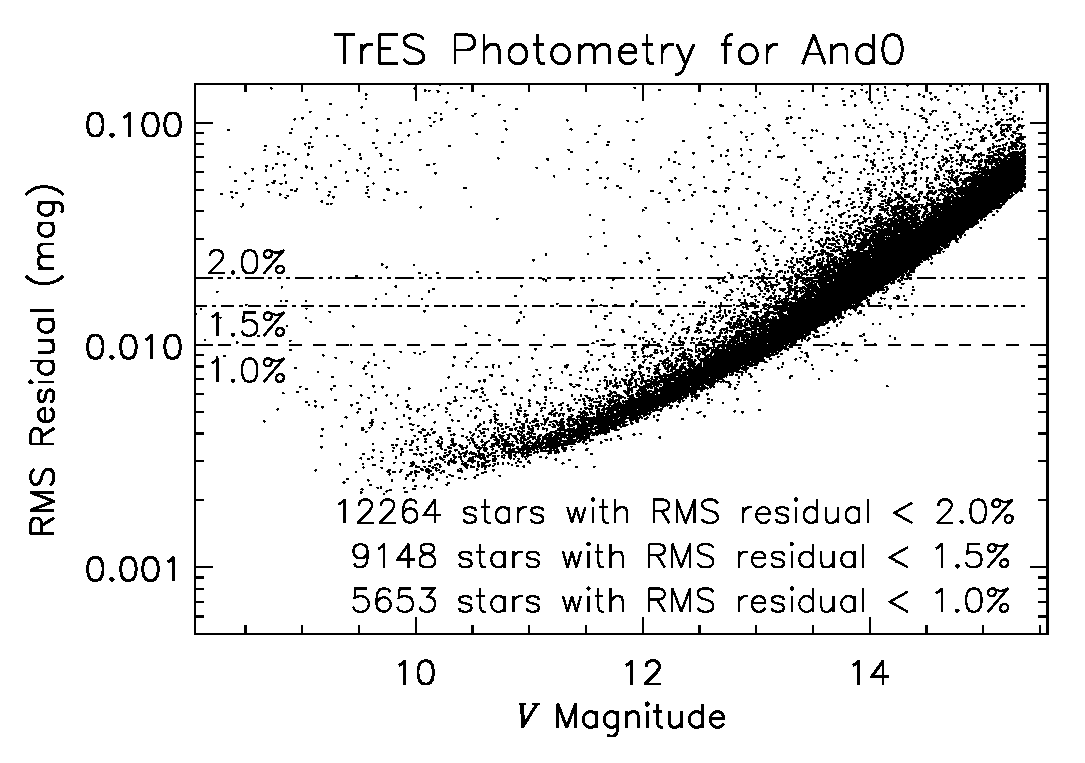
\includegraphics[width=0.95\textwidth]{2_f2}
\caption[Variation in rms residual with magnitude for And0 data]{Calculated rms residual of the binned data versus approximate $V$ magnitude for the stars in our TrES And0 data set. The number of stars with rms below 1\%, 1.5\%, and 2\% are shown.}\label{cha:and0:fig:rmsplot}
\end{center}
\end{figure}

\begin{figure}
\begin{center}
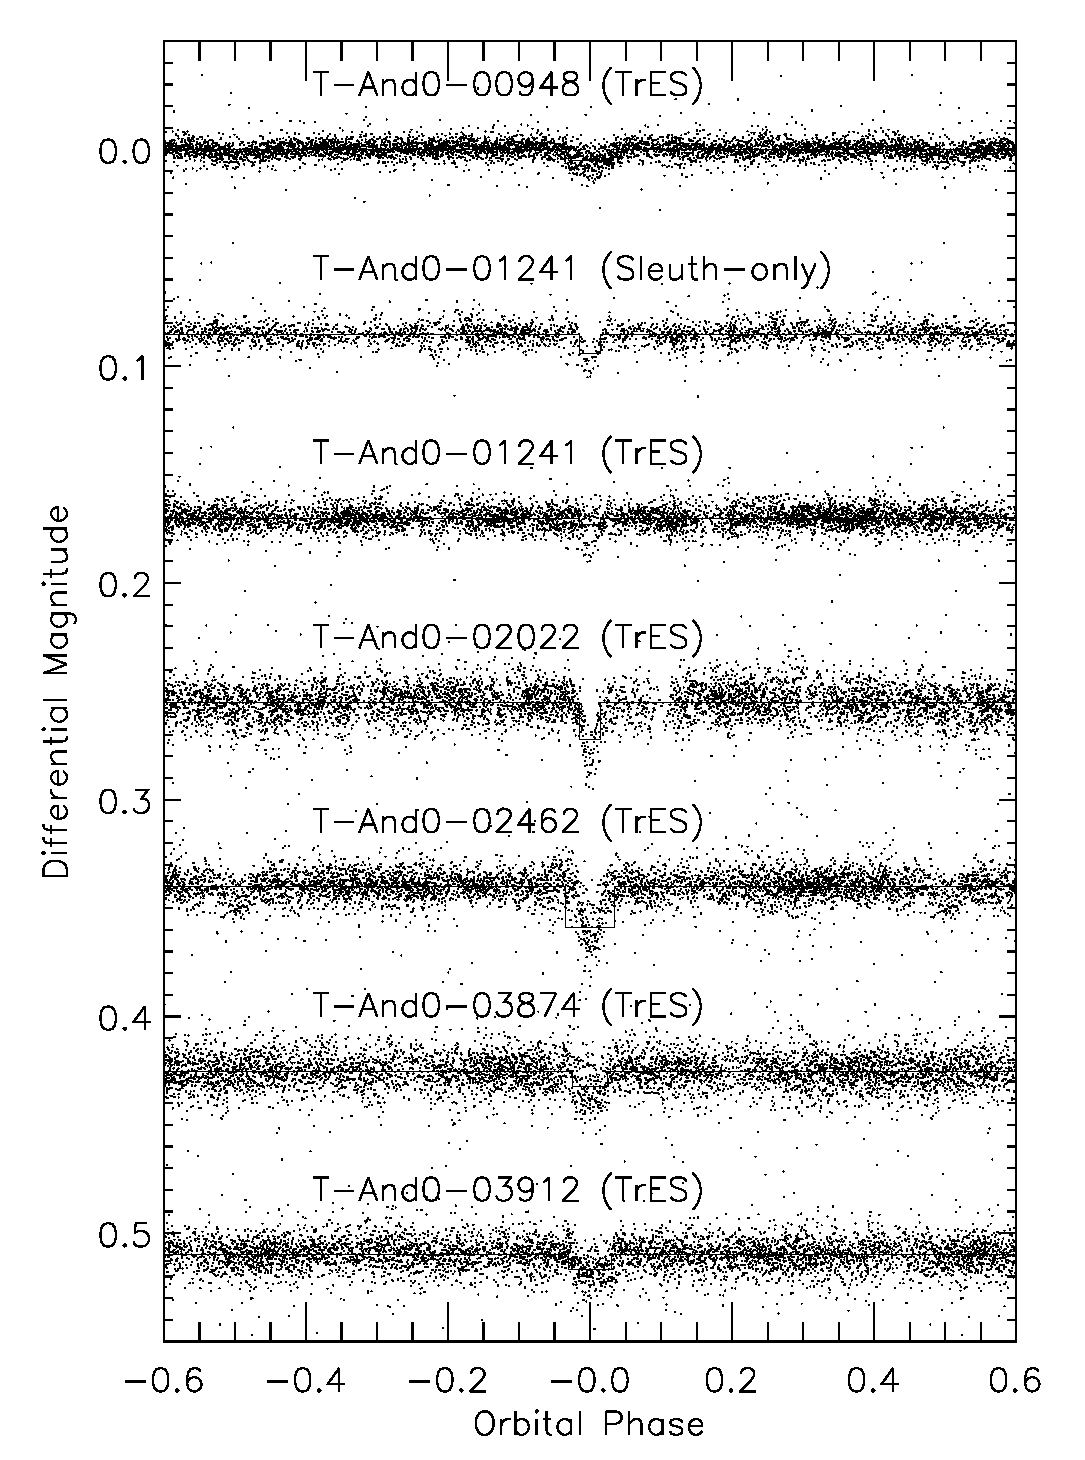
\includegraphics[width=0.95\textwidth]{2_f3}
\caption[TrES light curves of the six candidates from the And0 field]{Light curves of the six TrES candidates from the And0 field in Andromeda. The labels denote the source of the light curve. The timeseries have been phased to the best-fit period identified by the box-fitting algorithm of \citet{Kovacs_Zucker_Mazeh:aa:2002a} using the TrES data, with the exception of \mbox{T-And0-01241}, whose period was derived from the Sleuth data. The transit event is not present in the data from the other telescopes gathered at the same orbital phase.}\label{cha:and0:fig:tresCand}
\end{center}
\end{figure}

Initially, we examined our Sleuth observations separately, as these dominate the TrES data set, providing 50\% of the data. We binned the Sleuth time series using nine-minute bins to reduce computation time. The rms scatter of the binned data was below 0.015 mag for approximately 7800 stars. We searched the time series for periodic transit-like dips using the box-fitting least-squares transit-search algorithm (BLS; \citealt*{Kovacs_Zucker_Mazeh:aa:2002a}, see appendix~\ref{cha:bls}), which assigns a Signal Detection Efficiency (SDE) statistic to each star based on the strength of the transit detection. We restricted our search to periods ranging from 0.1 to 10 days. Having sorted the stars in order of decreasing magnitude and decreasing SDE, we visually examined each stellar light curve (phased to the best-fit period derived by the algorithm) in turn, until we determined that we could no longer distinguish a transit signal from the noise. We identified six transit candidates (see tables~\ref{cha:and0:tab:names} and~\ref{cha:and0:tab:transits}, and figure~\ref{cha:and0:fig:tresCand}).

We then combined the three TrES data sets, which optimized our visibility function (see figure~\ref{cha:and0:fig:vis}), and allowed us to confirm the detection of real eclipse events using simultaneous observations from multiple telescopes. We produced the combined TrES data set as follows. For each star in the Sleuth standard star list, we attempted to identify the corresponding stars in the other two lists. We computed the distances between a given Sleuth standard star and the PSST standard stars, and matched the Sleuth star with a PSST star if their angular separation was less than $5\arcsec$ (0.5 pixels). Because of the slight differences in the chosen filter and field of view, some Sleuth stars did not have corresponding PSST stars. We created a new standard star list from the Sleuth and PSST star lists, with only one entry for each pair of matched stars and an entry for each unmatched star. We then repeated this procedure with this new star list and the STARE list to produce the TrES field standard star list. For each star, we then combined the relevant time series, chronologically reordered the data, and binned the data. The rms scatter of the averaged TrES data was below 0.015\,mag for 9148 stars (see figure~\ref{cha:and0:fig:rmsplot}) out of the 29,259 stars in the field. We repeated the BLS transit search, but did not identify any new candidates. From figure~\ref{cha:and0:fig:vis}, we can see that a visibility of 80\% had already been achieved for $P<5$\,days for the Sleuth data alone, and the addition of the STARE and PSST data did not significantly increase the detection space for those short periods. The lack of additional candidates with these orbital periods is not surprising. However, for longer periods, the visibility for the TrES network is much better than for the single Sleuth telescope, yet we did not find new candidates with these periods. We proceeded to our follow-up observations of these six candidates with larger telescopes.

\section{Follow-up of Candidate Transiting Planets}\label{cha:and0:sec:followup}

\begin{deluxetable}{lcccccccc}
\rotate
\tablewidth{0pt}
\tablecaption{Photometric and spectroscopic properties of the six TrES And0 candidates%\label{cha:and0:tab:catalogs}}

\tablehead{
\colhead{Candidate} & \colhead{$v_{r}$ \tablenotemark{a}} & \colhead{$P(\chi^{2})$ \tablenotemark{b}} & \colhead{$T_{\mathrm{eff}}$ \tablenotemark{c}}  &  \colhead{$\log{g}$ \tablenotemark{c}}  & \colhead{$v\sin{i}$ \tablenotemark{c}}  & \colhead{$\mu$ \tablenotemark{d}} & \colhead{$B_{T}-V_{T}$  \tablenotemark{e}} & \colhead{$J-K_{s}$ \tablenotemark{f}}\\
\colhead{} & \colhead{($\mathrm{km\,s^{-1}}$)} & \colhead{} & \colhead{(K)} & \colhead{} & \colhead{($\mathrm{km\,s^{-1}}$)} & \colhead{($\mathrm{\mathrm{mas\,yr^{-1}}}$)} & \colhead{(mag)} & \colhead{(mag)}
}

\startdata
\tOne & $-28.82\pm\phn0.53$ & 0.180 & 5250 & 3.0 & \phn 3  &  3.0 &  \phs $0.87$  & $0.60$  \\
\tTwo & $-13.05\pm\phn4.06$ & \nodata &  9500 & 4.5 & 55 & 7.7 &  $-0.07$ & $0.01$  \\
\tThree & $\phm{-0}4.47\pm27.87$ & 0.000 & 7000 & 3.5 & 22 &  3.5 & \nodata & $0.24$   \\
\tFour & $-11.31\pm\phn4.73$ & 0.008 & 6250 & 3.5 & 77 & 5.5 & \nodata & $0.14$   \\
\tFive & $-15.41\pm\phn0.31$ & 0.747 & 5500 & 3.5 & \phn 2  & 6.0 & \nodata & $0.66$   \\
\tSix & $-35.26\pm\phn3.43$ & \nodata &  7750 & 3.5 & 88 & 8.2 & \nodata & $0.25$
\enddata
\tablenotetext{a}{The mean radial velocity.}
\tablenotetext{b}{The probability that the observed $\chi^2$ should be less than a value $\chi^{2}$, assuming that our model of a star without radial velocity variation is correct.}
\tablenotetext{c}{For a discussion of the errors in these spectroscopic data, see section~\ref{cha:and0:sec:reject}.}
\tablenotetext{d}{UCAC2 proper motions \citep{Zacharias_Urban_Zacharias:aj:2004a}.}
\tablenotetext{e}{Tycho-2 visible colors \citep{Hog_Fabricius_Makarov:aa:2000b, Hog_Fabricius_Makarov:aa:2000a}.}
\tablenotetext{f}{2MASS infrared colors \citep{Cutri_Skrutskie_van-Dyk:2003a}.}
\end{deluxetable}

Many of the bright stars within our field were also observed as part of other surveys. We identified our candidates in online catalogs and compared these observations with our expectations based on the planet hypothesis. We found Tycho-2 \citep{Hog_Fabricius_Makarov:aa:2000b, Hog_Fabricius_Makarov:aa:2000a} visible ($B_{T}-V_{T}$) colors for two of our candidates, and Two Micron All Sky Survey (2MASS; \citealt{Cutri_Skrutskie_van-Dyk:2003a}) infrared ($J-K_{s}$) colors for all six (see table~\ref{cha:and0:tab:catalogs}). We searched the USNO CCD Astrograph Catalog (UCAC2; \citealt{Zacharias_Urban_Zacharias:aj:2004a}) for the proper motions of the stars. All of the candidates display a measurable proper motion, consistent with nearby dwarfs. However, these proper motions were not sufficiently large to rule out distant, high-velocity giants. Finally, we retrieved Digitized Sky Survey%
\footnote{The {Digitized Sky Survey} (see \url{http://archive.stsci.edu/dss/}) was produced at the Space Telescope Science Institute under US Government grant NAG W-2166. The images of these surveys are based on photographic data obtained using the Oschin Schmidt Telescope on Palomar Mountain and the UK Schmidt Telescope. The plates were processed into the present compressed digital form with the permission of these institutions.}%
\ (DSS) images of the sky surrounding each candidate to check for possible nearby stars of similar brightness within our PSF radius. None were found.

We observed the six And0 candidates starting on UT 2004 September~28 using
the Harvard--Smithsonian Center for Astrophysics (CfA) Digital Speedometers \citep{Latham:ASP:1992a}. These spectrographs cover 45\,\AA\ centered on 5187\,\AA\, and have a resolution of $8.5\,\mathrm{km\,s^{-1}}$ (a resolving power of $\lambda / \Delta \lambda \approx 35,\!000$). We cross-correlated our spectra against a grid of templates from our library of synthetic spectra to estimate various stellar parameters of our targets and their radial velocities. J. Morse computed this spectral library, using the Kurucz model atmospheres (J.~Morse \& R.~L.~Kurucz, 2004, private communication).
Assuming a solar metallicity, we estimated the effective temperature ($T_{\mathrm{eff}}$), surface gravity ($g$), and rotational velocity ($v \sin{i}$) for each candidate (see table~\ref{cha:and0:tab:catalogs}) from the template parameters that gave the highest average peak correlation value over all the observed spectra.

\begin{deluxetable}{cccc}
\rotate
\tablewidth{0pt}
\tablecaption{Details of spectroscopic observations of the six TrES And0 candidates\label{cha:and0:tab:rv}}
\tablehead{
\colhead{Candidate} & \colhead{Time of Observation} & \colhead{Photometric Orbital Phase} & \colhead{Radial Velocity} \\
\colhead{} & \colhead{HJD} & \colhead{} & \colhead{$\mathrm{km\,s^{-1}}$}
}

\startdata
\multirow{3}{*}{\tOne}   & 2453276.8749 & 0.46  & $-28.16 \pm 0.36$ \\
 & 2453277.8530 & 0.33 & $-29.19 \pm 0.40$ \\
 & 2453278.8236 & 0.20 & $-29.00 \pm 0.32$ \\
 & & \\
\tTwo    & 2453276.8062 & 0.73 & $-13.05 \pm 4.06$ \\
 & & \\
\multirow{16}{*}{\tThree}  & 2453276.8642 & 0.80 & $\phm{-}35.46 \pm 0.74$ \\
 & 2453301.8475 & 0.07 & $-14.14 \pm 0.99$ \\
 & 2453334.7734 & 0.02 & $-\phn3.77 \pm 0.94$ \\
 & 2453548.9711 & 0.21 & $-39.63 \pm 1.12$ \\
 & 2453575.9740 & 0.90 & $\phm{-}24.54 \pm 1.05$ \\
 & 2453576.9683 & 0.11 & $-20.34 \pm 1.16$ \\
 & 2453626.9029 & 0.65 & $\phm{-}23.98 \pm 1.13$ \\
 & 2453627.9043 & 0.86 & $\phm{-}29.37 \pm 0.70$ \\
 & 2453628.8392 & 0.06 & $-\phn9.31 \pm 0.81$ \\
 & 2453629.8518 & 0.27 & $-42.28 \pm 1.12$ \\
 & 2453630.8361 & 0.48 & $-15.29 \pm 1.24$ \\
 & 2453631.8335 & 0.69 & $\phm{-}30.93 \pm 0.86$ \\
 & 2453632.8135 & 0.90 & $\phm{-}24.80 \pm 0.87$ \\
 & 2453633.8047 & 0.10 & $-20.66 \pm 1.02$ \\
 & 2453636.8830 & 0.75 & $\phm{-}37.44 \pm 0.86$ \\
 & 2453779.5864 & 0.84 & $\phm{-}29.64 \pm 1.14$ \\
\multirow{2}{*}{\tFour}   & 2453276.8864 & 0.11 & $-\phn7.55 \pm 1.40$ \\
 & 2453686.7688 & 0.18 & $-14.50 \pm 3.74$ \\
 & & \\
\multirow{4}{*}{\tFive}    & 2453276.8192 & 0.17 & $-15.81 \pm 0.44$ \\
 & 2453277.8381 & 0.55 & $-15.15 \pm 0.41$ \\
 & 2453301.8342 & 0.59 & $-15.09 \pm 0.43$ \\
 & 2453334.7619 & 0.00 & $-15.50 \pm 0.43$ \\
 & & \\
\tSix      & 2453276.8398 & 0.22 & $-35.26 \pm 3.43$ \\
\enddata
\end{deluxetable}

For the three candidates with low stellar rotation, $v\sin{i} < 50\,\mathrm{km\,s^{-1}}$, we obtained several spectra over different observing seasons to determine the radial velocity variation of each star. Table~\ref{cha:and0:tab:rv} details our spectroscopic observations. For these slowly rotating candidates, the typical precision for our spectroscopic parameters is $\Delta T_{\mathrm{eff}} = 150\,\mathrm{K}$, $\Delta \log{g} = 0.5$, $\Delta v \sin{i} = 2\,\mathrm{km\,s^{-1}}$, and $\Delta V = 0.5\,\mathrm{km\,s^{-1}}$. The precision of the estimates degrades for stars with large $v\sin{i}$ values or few spectroscopic observations.

We obtained high-precision photometry of \tFive\ on UT 2004 December~19 using the Minicam CCD imager at the FLWO 1.2-meter telescope on
Mount Hopkins, Arizona.  Minicam consists of two $2248\times 4640$ pixels
thinned, backside-illuminated Marconi CCDs mounted side-by-side to
span a field of approximately $20.4\arcmin \times 23.1 \arcmin$ bisected by
a narrow gap.  We employed $2 \times 2$ pixels binning for an effective
plate scale of $0.6\arcsec\,\mathrm{pixel}^{-1}$ and read out each half CCD
through a separate amplifier.  We offset the telescope to place
\tFive\ centrally on one amplifier region and autoguided on the
field.  We obtained concurrent light curves in three filters by cycling
continuously through the SDSS $g$, $r$, and $z$ filters with exposure times
of 90, 45, and 90\,s respectively.  The seeing was poor
(FWHM $\sim3\arcsec$--$7\arcsec$) and varied throughout our observations.
Unfortunately, high winds forced us to close the dome during the night
and we obtained only partial coverage of the predicted event.  Late in
the scheduled observations, we re-opened for a short time.

We subtracted the overscan bias level from each image and divided each
by a normalized flat field constructed from the filtered mean of
twilight sky exposures.  To construct a light curve of \tFive\ and neighboring
bright stars, we located the stars in each image.  We measured stellar fluxes in a
circular aperture and subtracted the sky as estimated by the median
flux in an annulus centered on the star (iteratively rejecting deviant
sky pixel values).  We used a relatively large 12$\arcsec$ radius
aperture and sky annulus with inner and outer radii of 15$\arcsec$ and 27$\arcsec$
respectively in an effort to reduce systematic errors
arising due to the poor and variable seeing conditions.
We first corrected the flux of each star by an amount proportional to its
air mass in each exposure by using extinction coefficients for each
filter based on previous experience with Minicam photometry.
Second, we selected a group of bright, uncrowded stars near \tFive\ as
potential comparison stars.  In each exposure we calculated the mean flux
of the comparison stars weighted according to brightness.  We assumed
that any variations in this mean flux represented extinction in each image
and used them to apply corrections to each light curve.  We then
inspected by eye the light curve of each comparison star and fit the light curves to
models of constant brightness to find $\chi^2$ statistics. We
removed from our group of comparison stars any star that showed significant
variations. We recalculated the extinction corrections iteratively in
this manner until we achieved no variation in the comparison star light curves.
We accepted 29, 32, and 4 comparison stars for the $g$-, $r$-, and $z$-band light curves respectively. Finally, we normalized the flux in the light curves of \tFive\ with respect to the out-of-eclipse data.

\section{Rejecting False-Positive Detections}\label{cha:and0:sec:reject}

Based on our detailed investigations of the candidates, we eliminated each And0 candidate as follows.

In the case of \tOne, the TrES light curve (figure~\ref{cha:and0:fig:tresCand}) shows a secondary eclipse. The low surface gravity ($\log{g}=3.0$) is that of a distant giant star, consistent with the red color $J-K_{s}=0.60$\,mag (since the majority of stars with $J-K_{s}>0.5$\,mag are expected to be giants, \citealp[see, e.g.,][]{Brown:apjl:2003a}). There was no observed variation in the radial velocity of this candidate ($v_r=-28.82\,\mathrm{km\,s^{-1}}$). \tOne\ is most likely the primary star of a diluted triple system.

\begin{figure}
\begin{center}
\centering
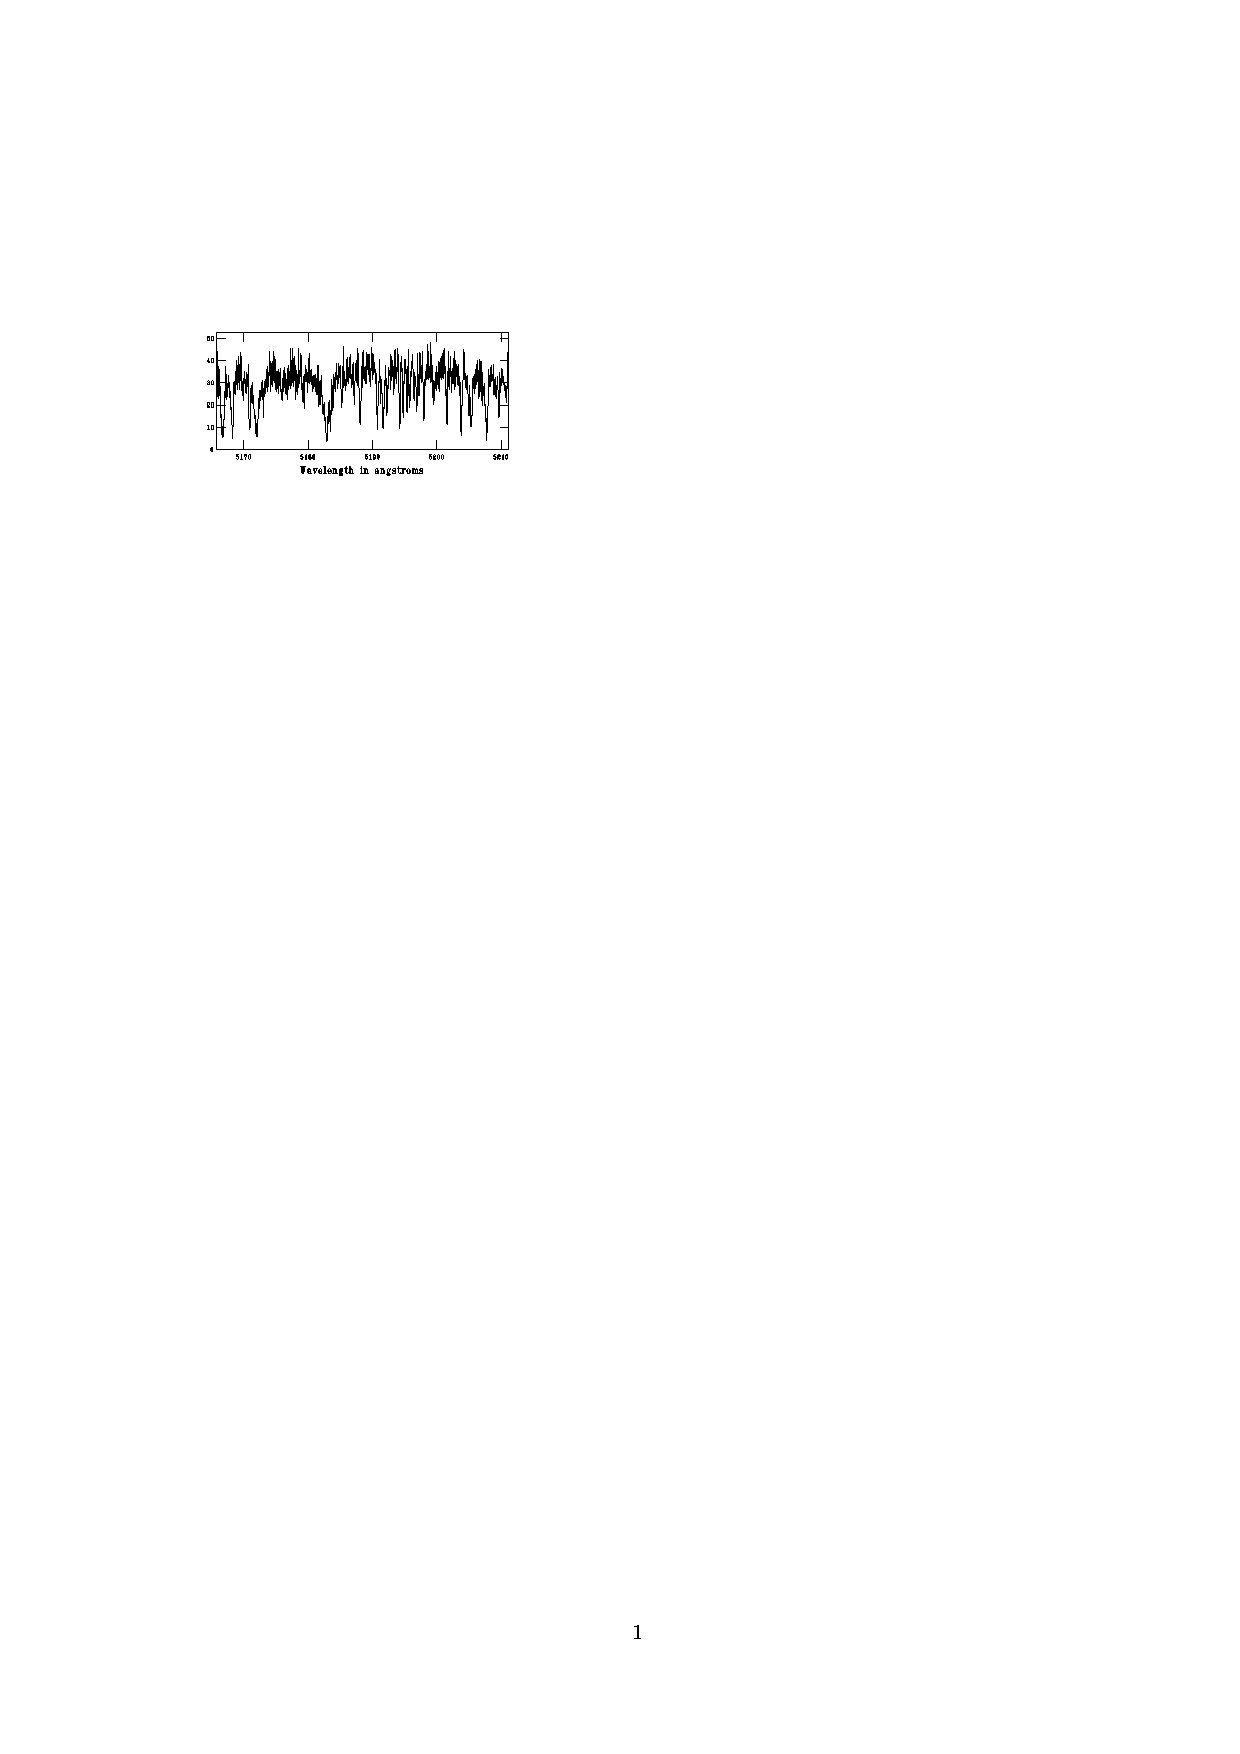
\includegraphics[width=.45\textwidth]{2_f4a}
\hspace{1cm}
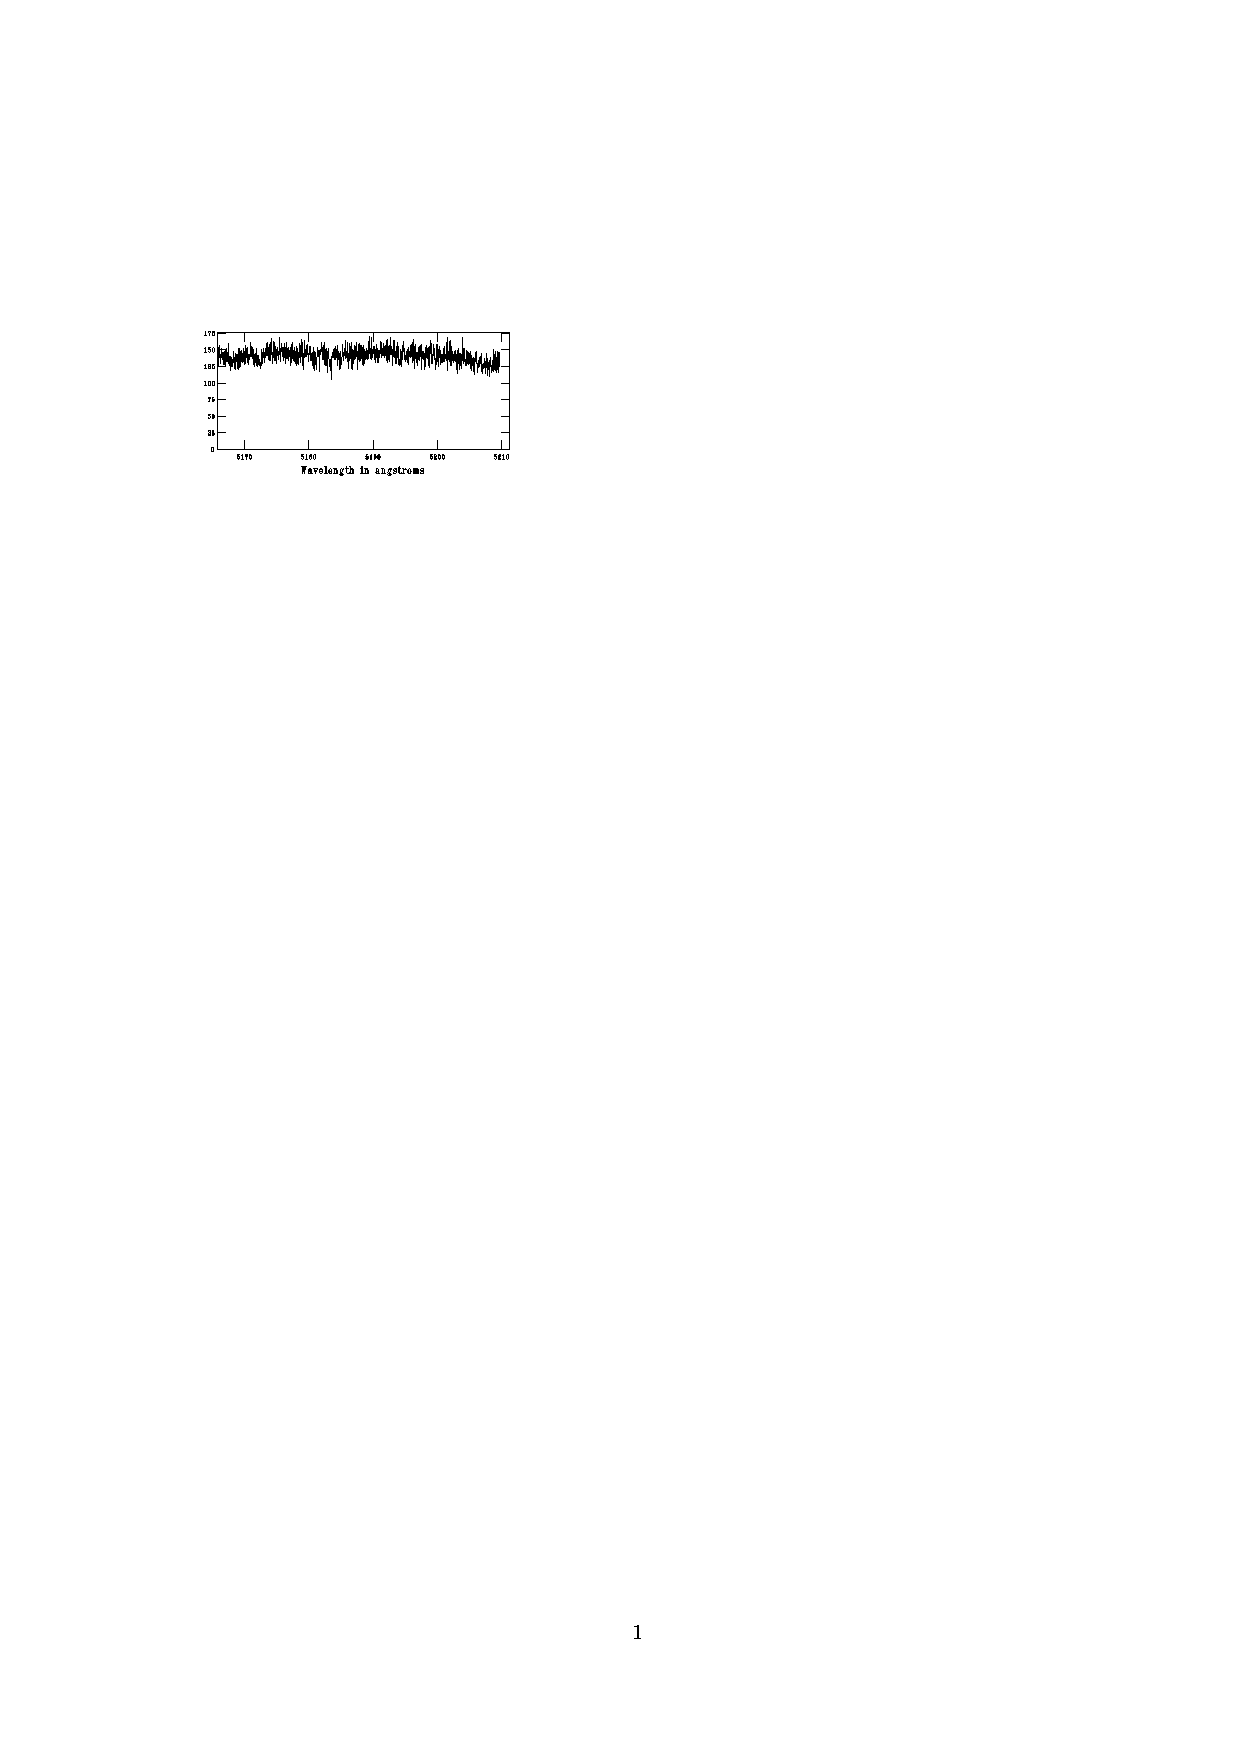
\includegraphics[width=.45\textwidth]{2_f4b}\\
\textsc{\small $(a)$    \hspace{7cm}    $(b)$}\\
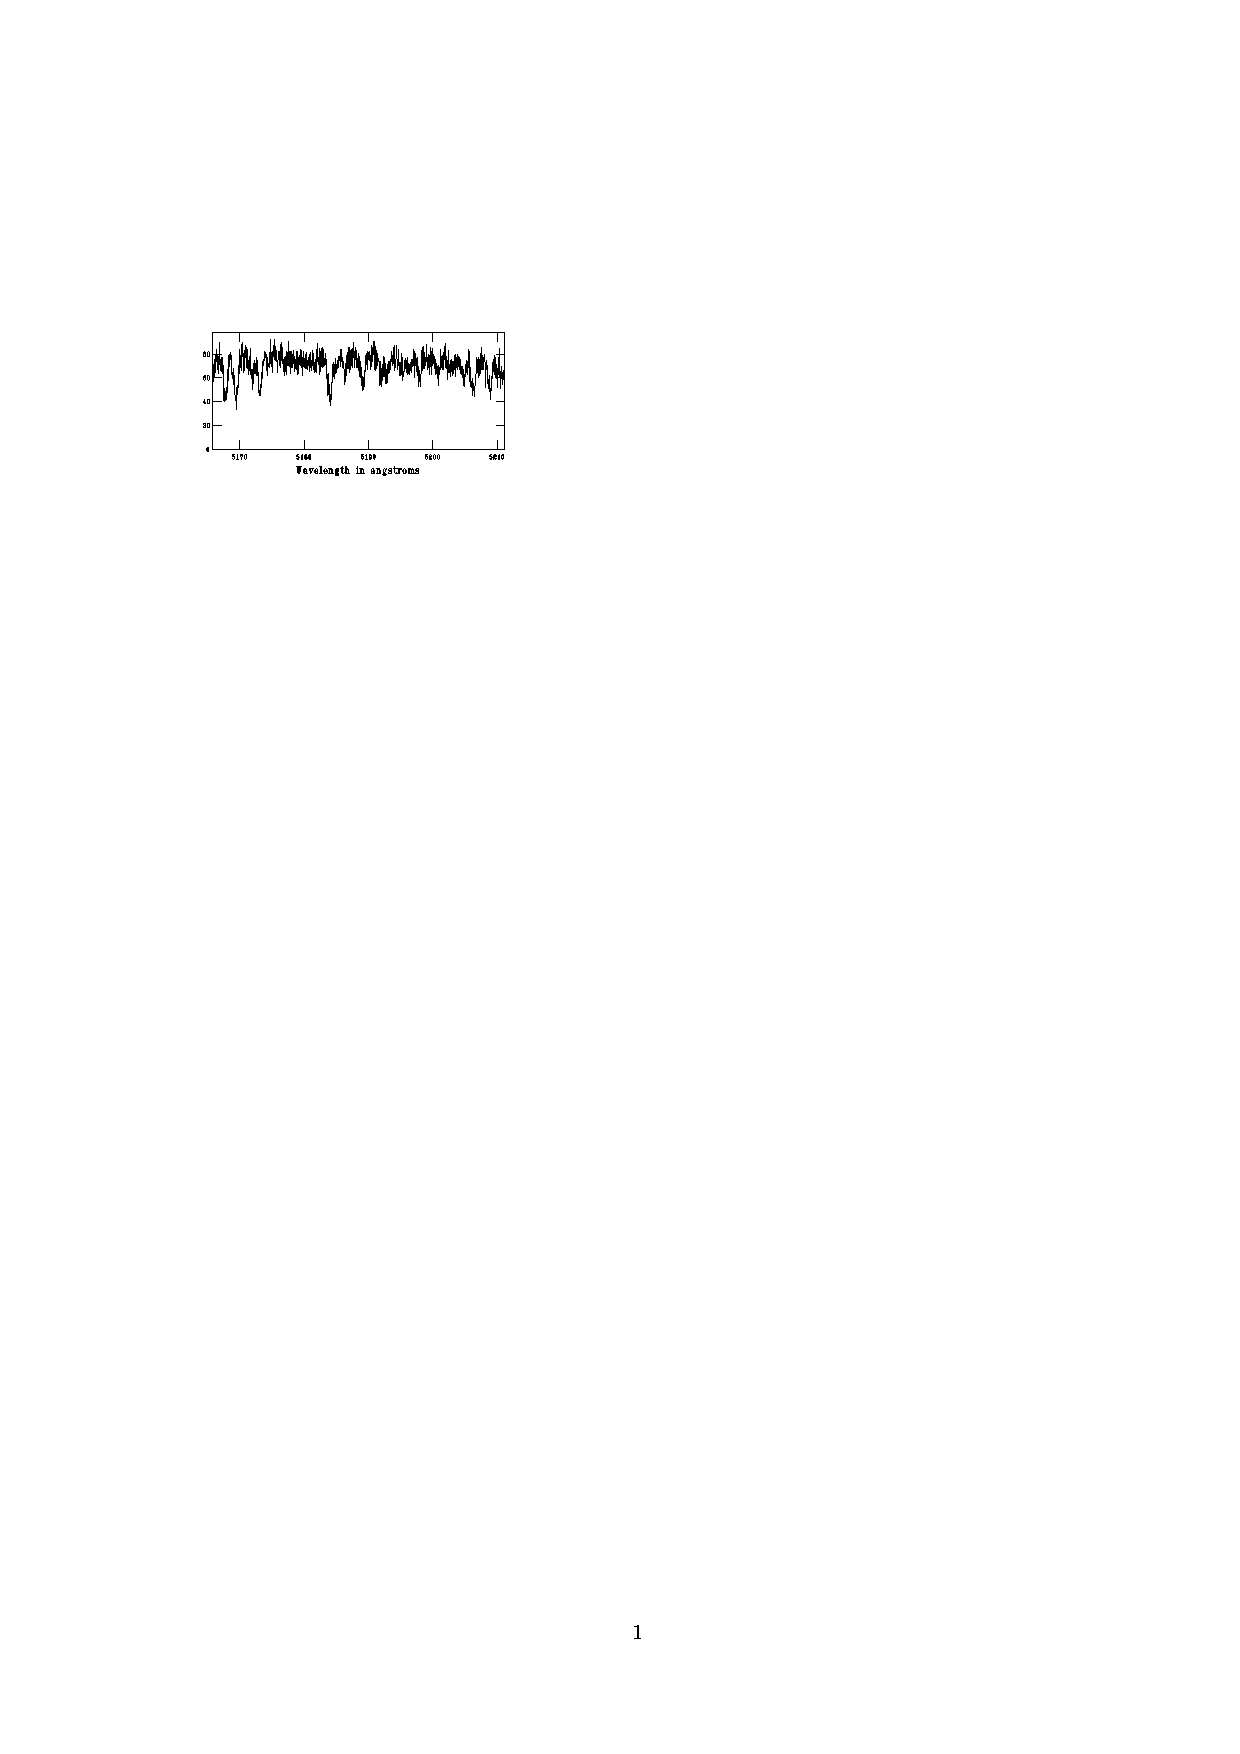
\includegraphics[width=.45\textwidth]{2_f4c}
\hspace{1cm}
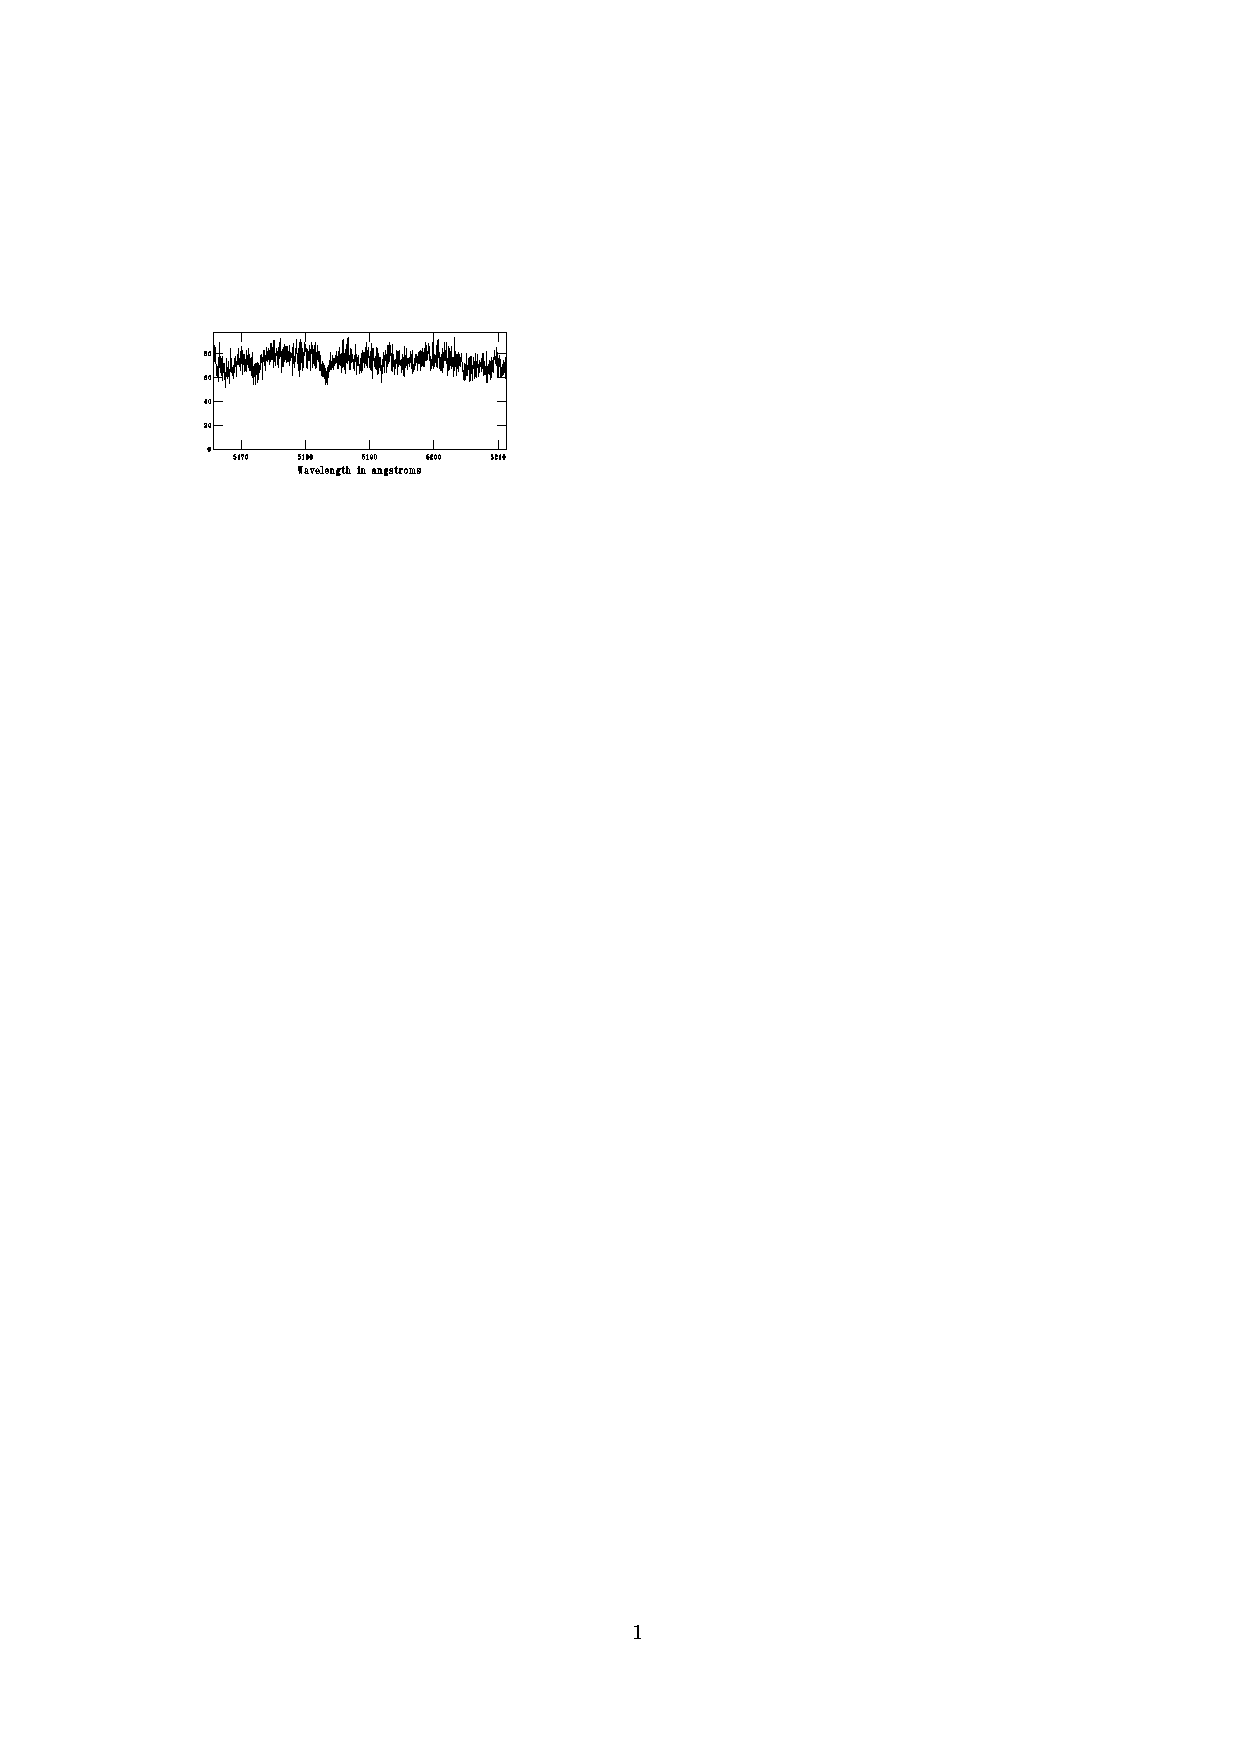
\includegraphics[width=.45\textwidth]{2_f4d}\\
\textsc{\small $(c)$    \hspace{7cm}    $(d)$}\\
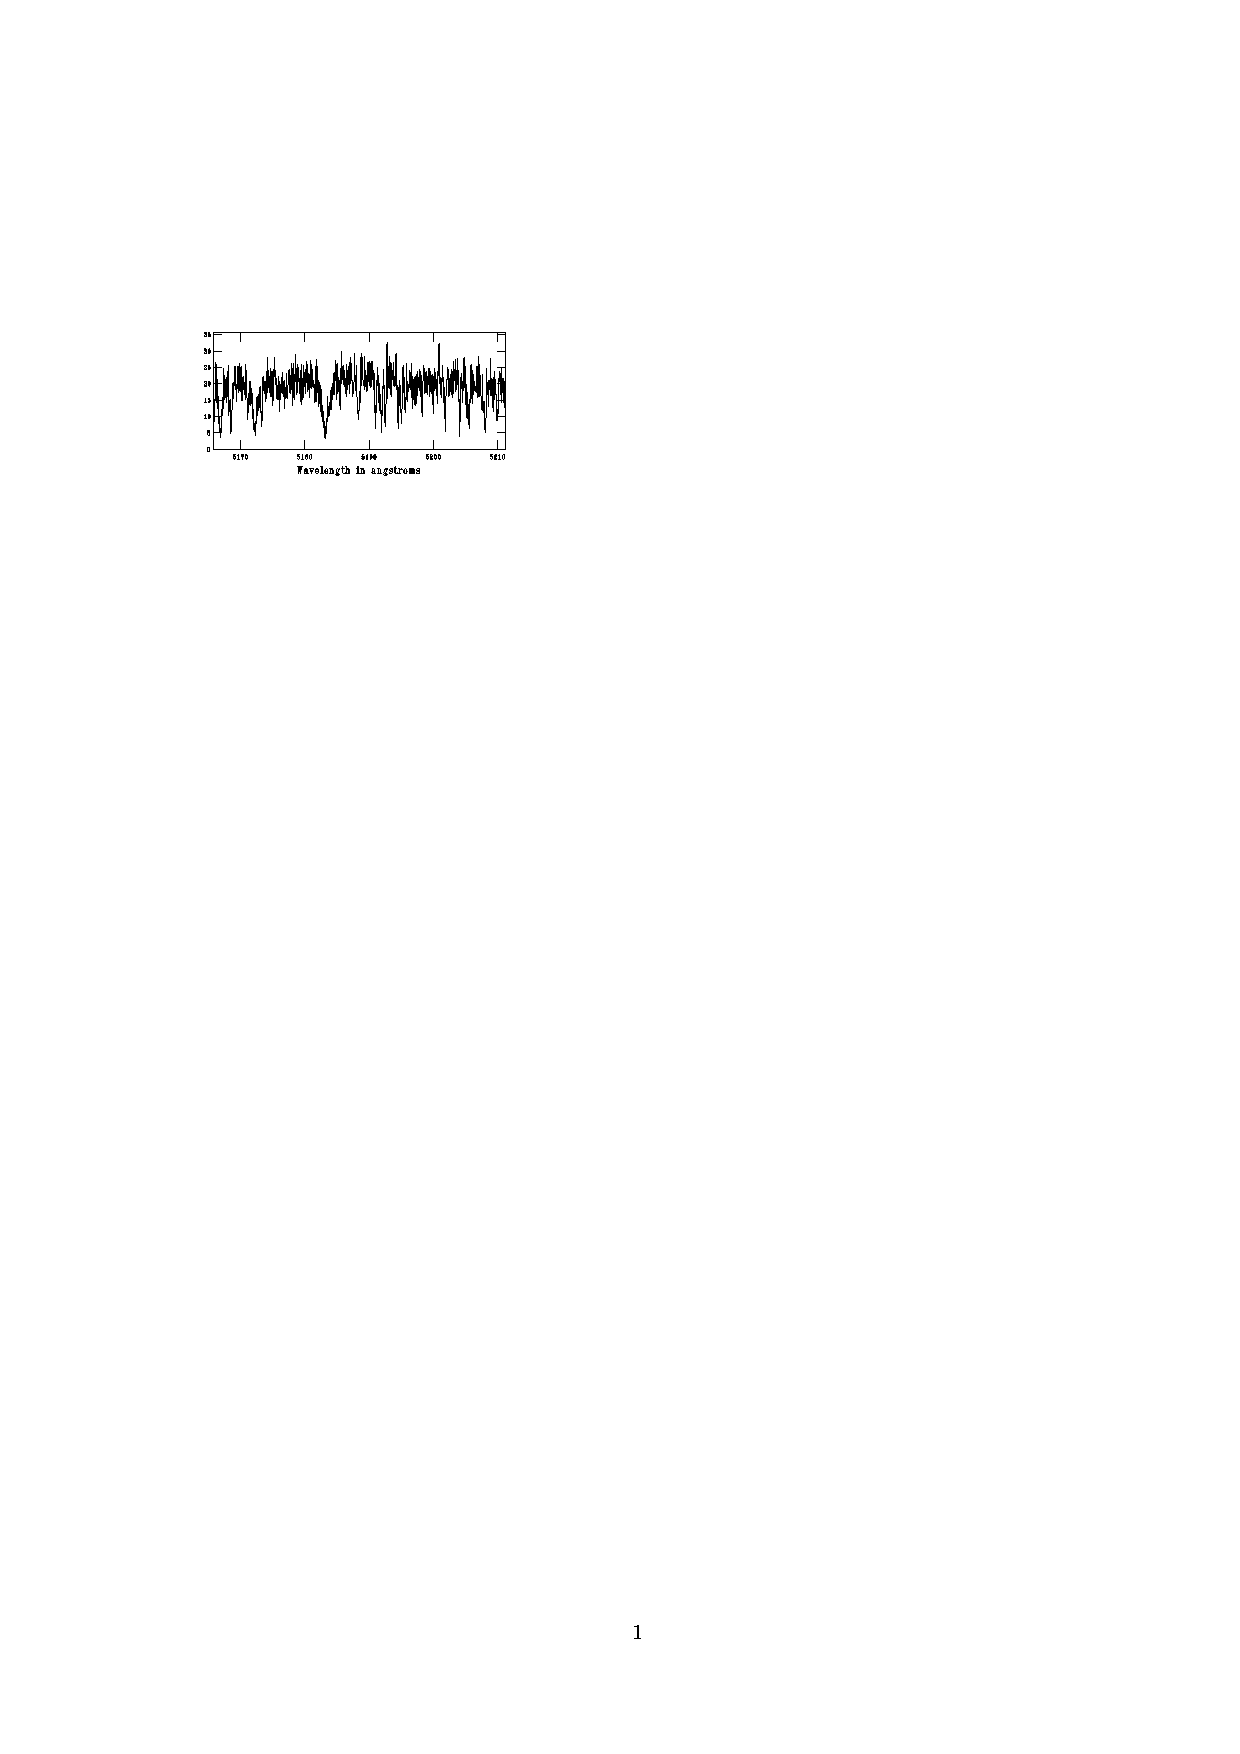
\includegraphics[width=.45\textwidth]{2_f4e}
\hspace{1cm}
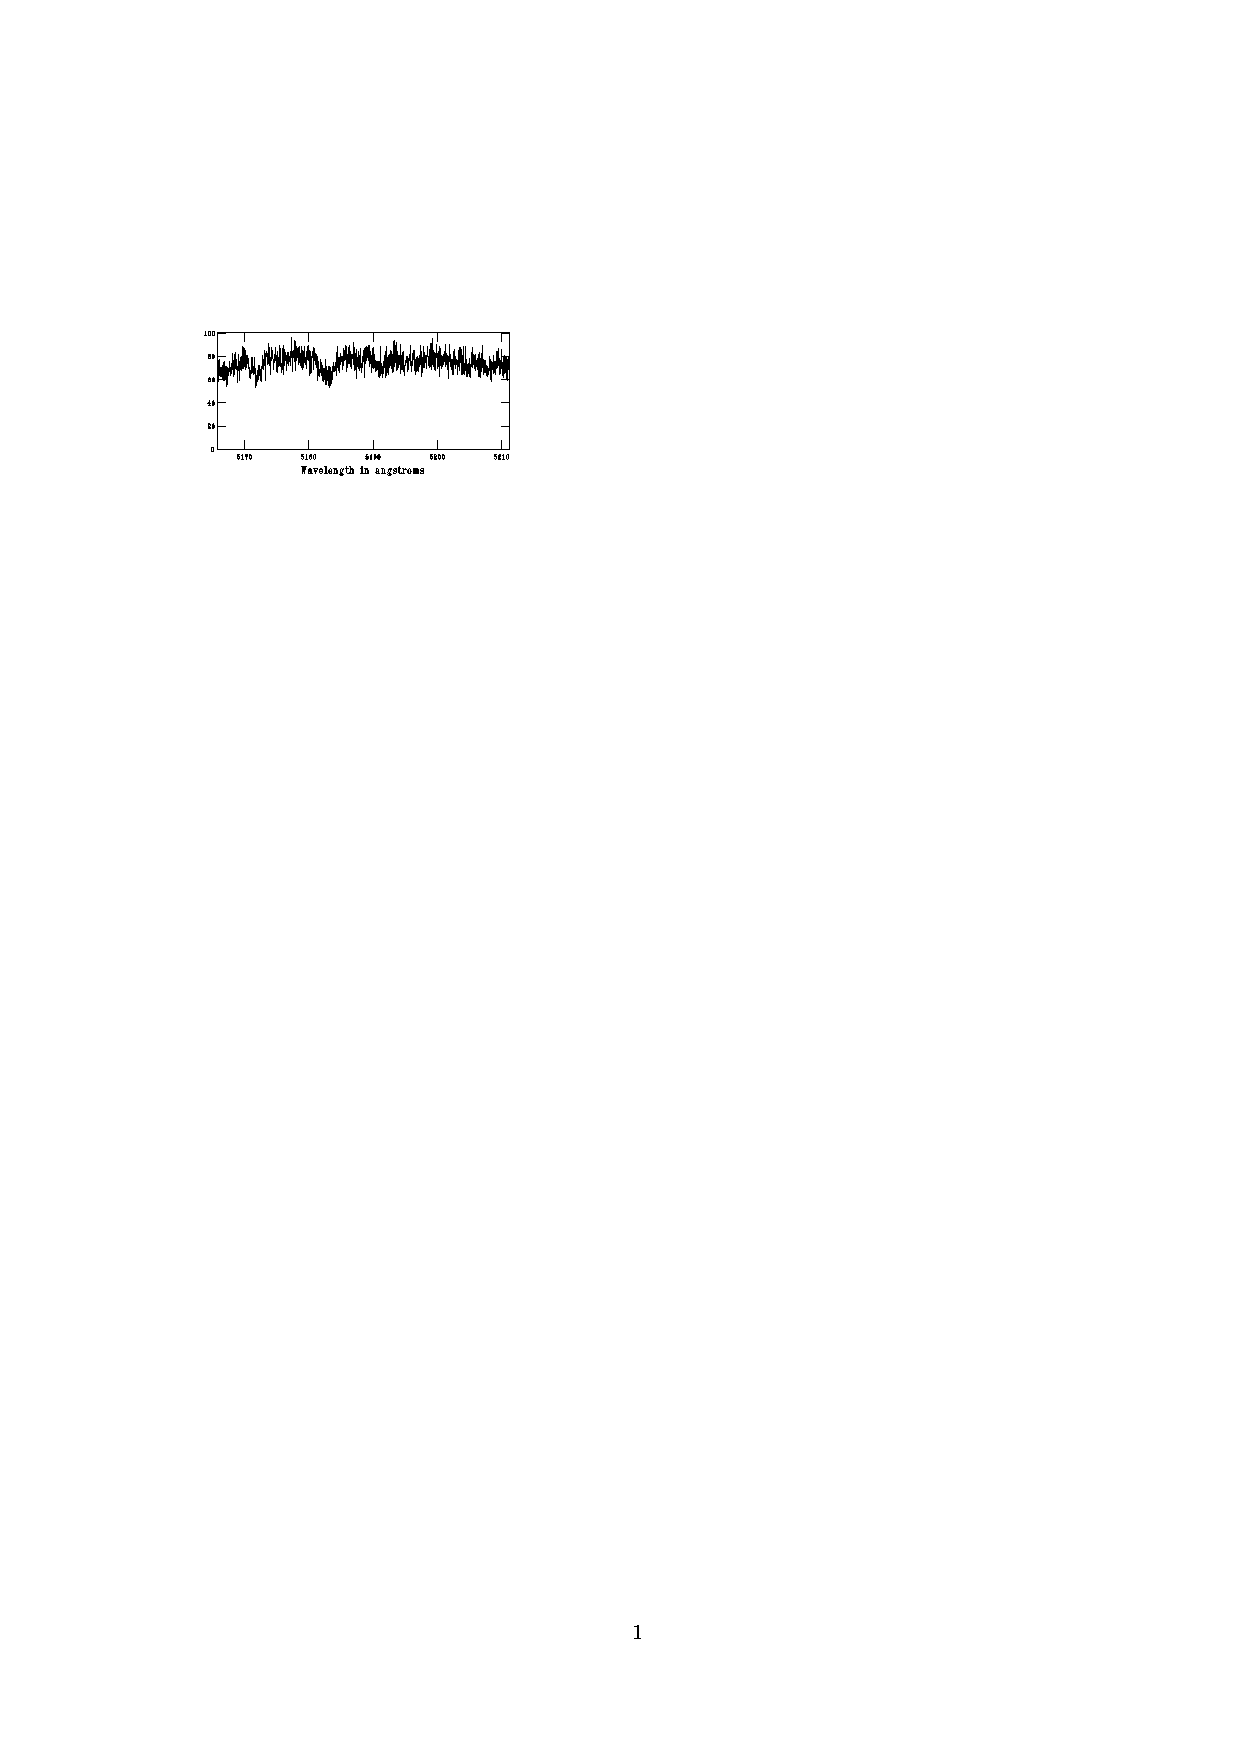
\includegraphics[width=.45\textwidth]{2_f4f} \\
\textsc{\small $(e)$    \hspace{7cm}    $(f)$}
\caption[Sample spectra of the And0 transit candidates]{
Sample spectra of the And0 TrES candidates obtained with the CfA Digital Speedometers on the FLWO 1.5-meter telescope: ($a$) \mbox{T-And0-00948} has the low surface gravity of a giant star, ($b$) \mbox{T-And0-01241} has the featureless spectrum of an A-type star, ($c$) \mbox{T-And0-02022} is an evolved F dwarf,  ($d$) \mbox{T-And0-02462} and ($e$) \mbox{T-And0-03912} display broadened lines due to the rapid rotation of these stars, and ($f$) \mbox{T-And0-03874} is an early K-type dwarf.
}\label{cha:and0:fig:spectra}
\end{center}
\end{figure}

Upon further examination of the individual light curves for \tTwo, we noticed that only Sleuth had observed transit events for this system. Neither PSST nor STARE had observed this field during the time of the Sleuth transit events, preventing a comparison of the light curves. Based on the Sleuth data, we predicted the times of transits during the entire TrES And0 campaign. STARE did observe \tTwo\ at a time at which it was predicted to transit but did not observe the transit. It was therefore possible that this was a photometric false positive. However, we did not pursue this further, as we obtained sufficient evidence from the follow-up spectroscopy to discount the system. A dwarf with $\log{g}=4.5$, the star has the high effective temperature ($T_{\mathrm{eff}}=9500$\,K) and blue colors ($J-K_{s}=0.01$\,mag) of an early A star. Figure~\ref{cha:and0:fig:spectra}$b$ shows the nearly featureless spectrum of this star. For such a large star with a radius $R\sim2.7\,R_{\sun}$, the observed transit depth of 0.9\% indicates a non-planetary size ($R=2.5\,R_{\mathrm{Jup}}$) for the eclipsing body.

\begin{figure}
\begin{center}
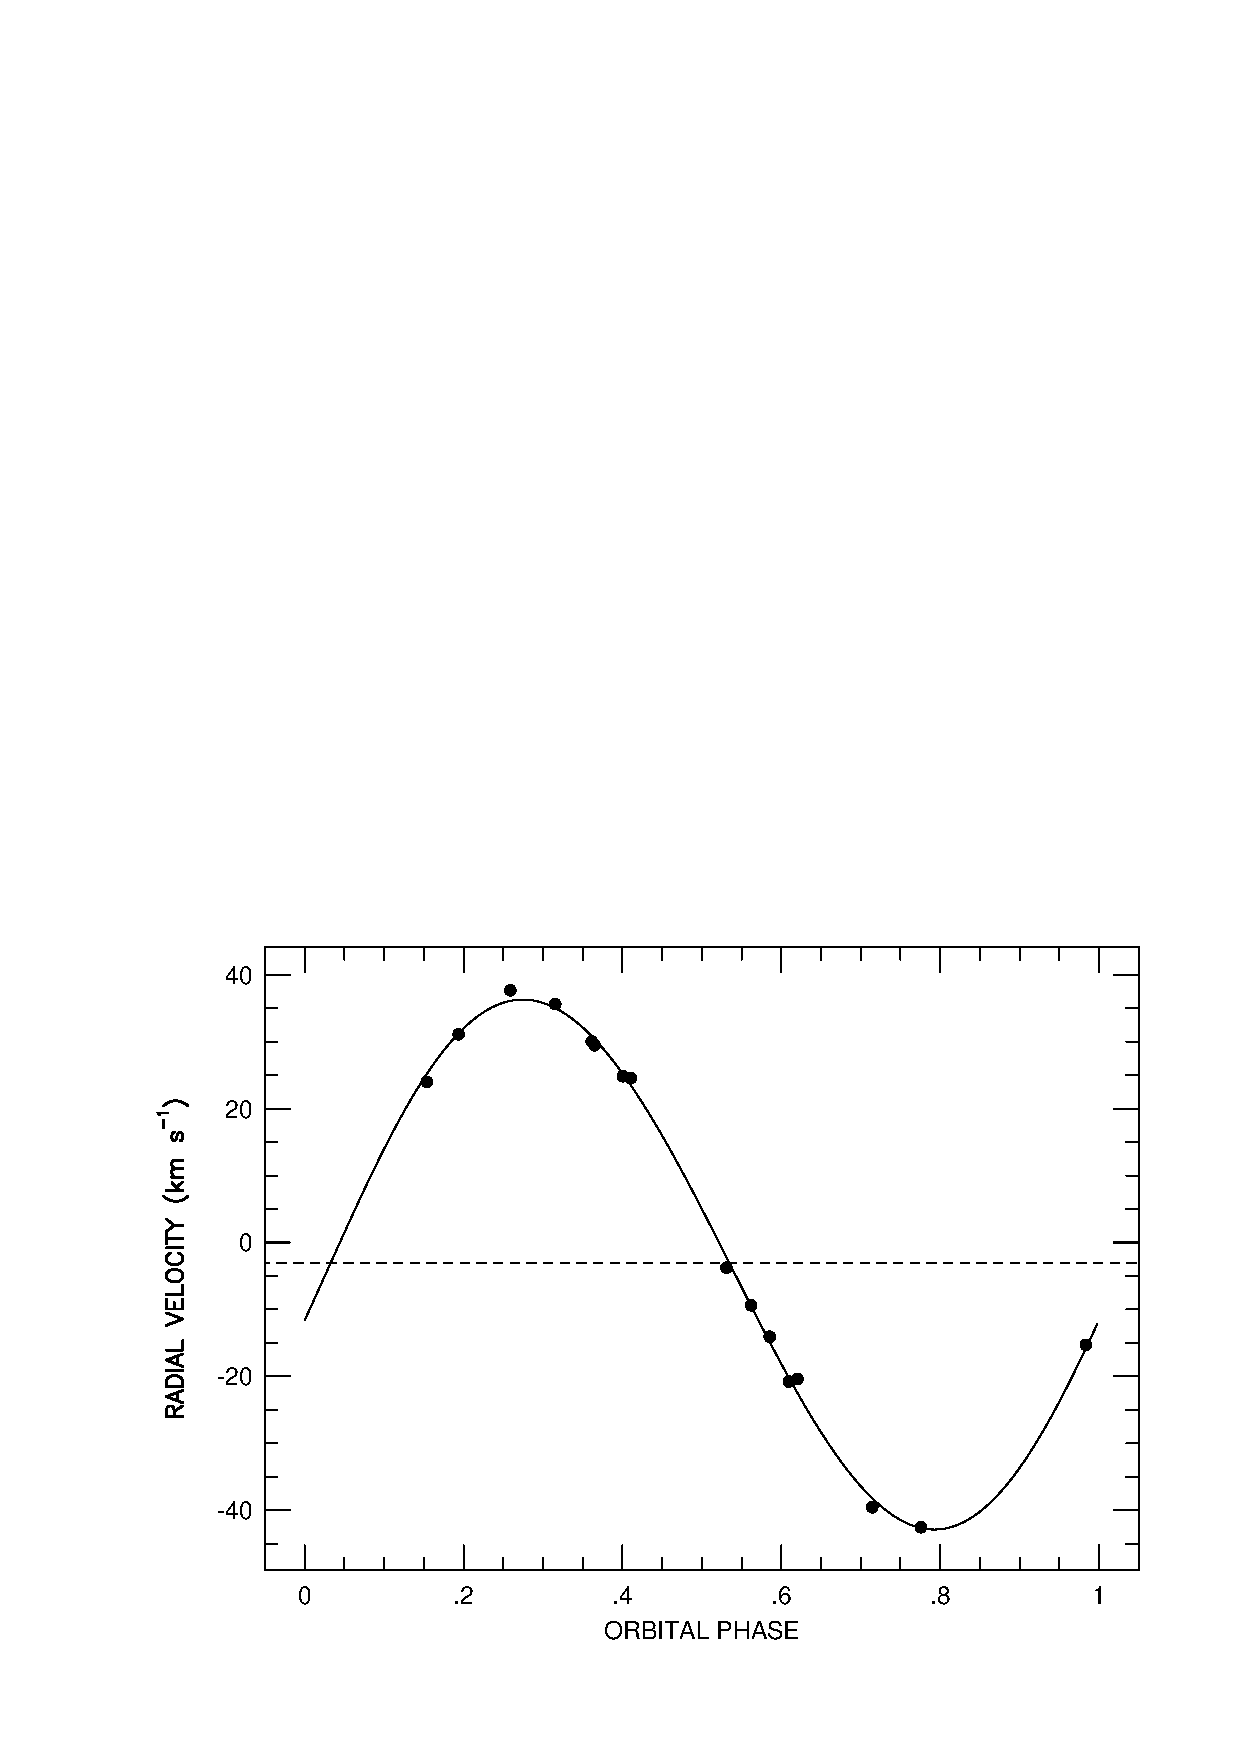
\includegraphics[width=0.95\textwidth]{2_f5}
\caption[Radial velocity orbit of \mbox{T-And0-02022}, an F+M eclipsing binary]{
Radial velocity orbit of \mbox{T-And0-02022} as determined from our Digital Speedometer spectra. This system was quickly rejected as a candidate transiting planet after the large radial velocity variation was determined from initial spectroscopic observations. Additional epochs produced a precise orbit with an eccentricity of $e\sim0.03$. An initial mass estimate of $0.5\,\mathrm{M}_{\sun}$ was derived for the companion. Future photometry will lead to more precise mass determination for both component stars (see text for a discussion).}\label{cha:and0:fig:rvorbit}
\end{center}
\end{figure}

The radial velocity of \tThree\ varies with an amplitude corresponding to a stellar-mass companion. We determined this system to be an eclipsing binary, comprising a slightly evolved F dwarf and an M dwarf. This system has a mass function $f(M)=0.0304\pm0.0013\,\mathrm{M}_{\sun}$ and an eccentricity of $0.027\pm0.014$. Assuming an orbital inclination of $i\sim90\degr$ and a mass of $1.6\,\mathrm{M}_{\sun}$ consistent with the effective temperature ($T_{\mathrm{eff}}=7000$\,K), we estimated the mass of the companion to be $m=0.5\,\mathrm{M}_{\sun}$. Figure~\ref{cha:and0:fig:rvorbit} shows the radial velocity orbit. The circular orbit of \tThree\ allows us to constrain the stellar radius, independent of our derived spectral type and luminosity class. The circular orbit implies orbital synchronization and orbital-rotation axes alignment, since circularization has the longest timescale of these processes. (This should apply except for very low mass secondaries; \citealp[see][]{Hut:aa:1981a} for a derivation of these timescales for close binary systems and a comparison for different binary mass ratios and moments of inertia of the primary star.) We can therefore assume that the stellar rotation period is the same as the orbital period of $4.7399$\,days. We then use the observed rotational broadening ($v\sin{i}=22\,\mathrm{km\,s^{-1}}$) to estimate the radius of the star to be $2.0\,R_{\sun}$. Future photometric observations of this systems with KeplerCam \citep{Szentgyorgyi_Geary_Latham:AAS:2005a} are planned to more precisely measure the eclipse depth and to derive the radius and true mass of each star in this binary (J.~M.~Fern\'{a}ndez~et~al. 2007, in preparation).

\tFour\ is a rapid rotator with $v\sin{i}=77\,\mathrm{km\,s^{-1}}$ and displays rotationally broadened lines (see figure~\ref{cha:and0:fig:spectra}$d$), limiting the possibility of detecting the radial velocity variation caused by a planet. Regardless, we inferred a binary nature for this candidate using the combined TrES data, which proved essential in identifying this false positive. Our initial Sleuth light curve of \tFour\ showed no evidence of a stellar-mass companion, and we derived a BLS best-fit period of 1.5347\,days. On examining the TrES light curve of \tFour\ (see figure~\ref{cha:and0:fig:tresCand}), we noticed a secondary eclipse. Also, the BLS best-fit period for our TrES observations of \tFour\ is twice that derived from the Sleuth data alone. When we reexamined the Sleuth data phased to the TrES period, the secondary eclipse is not visible due to inadequate coverage at that phase. This resulted in a derived period for the Sleuth data half that of the true period.

\begin{figure}
\begin{center}
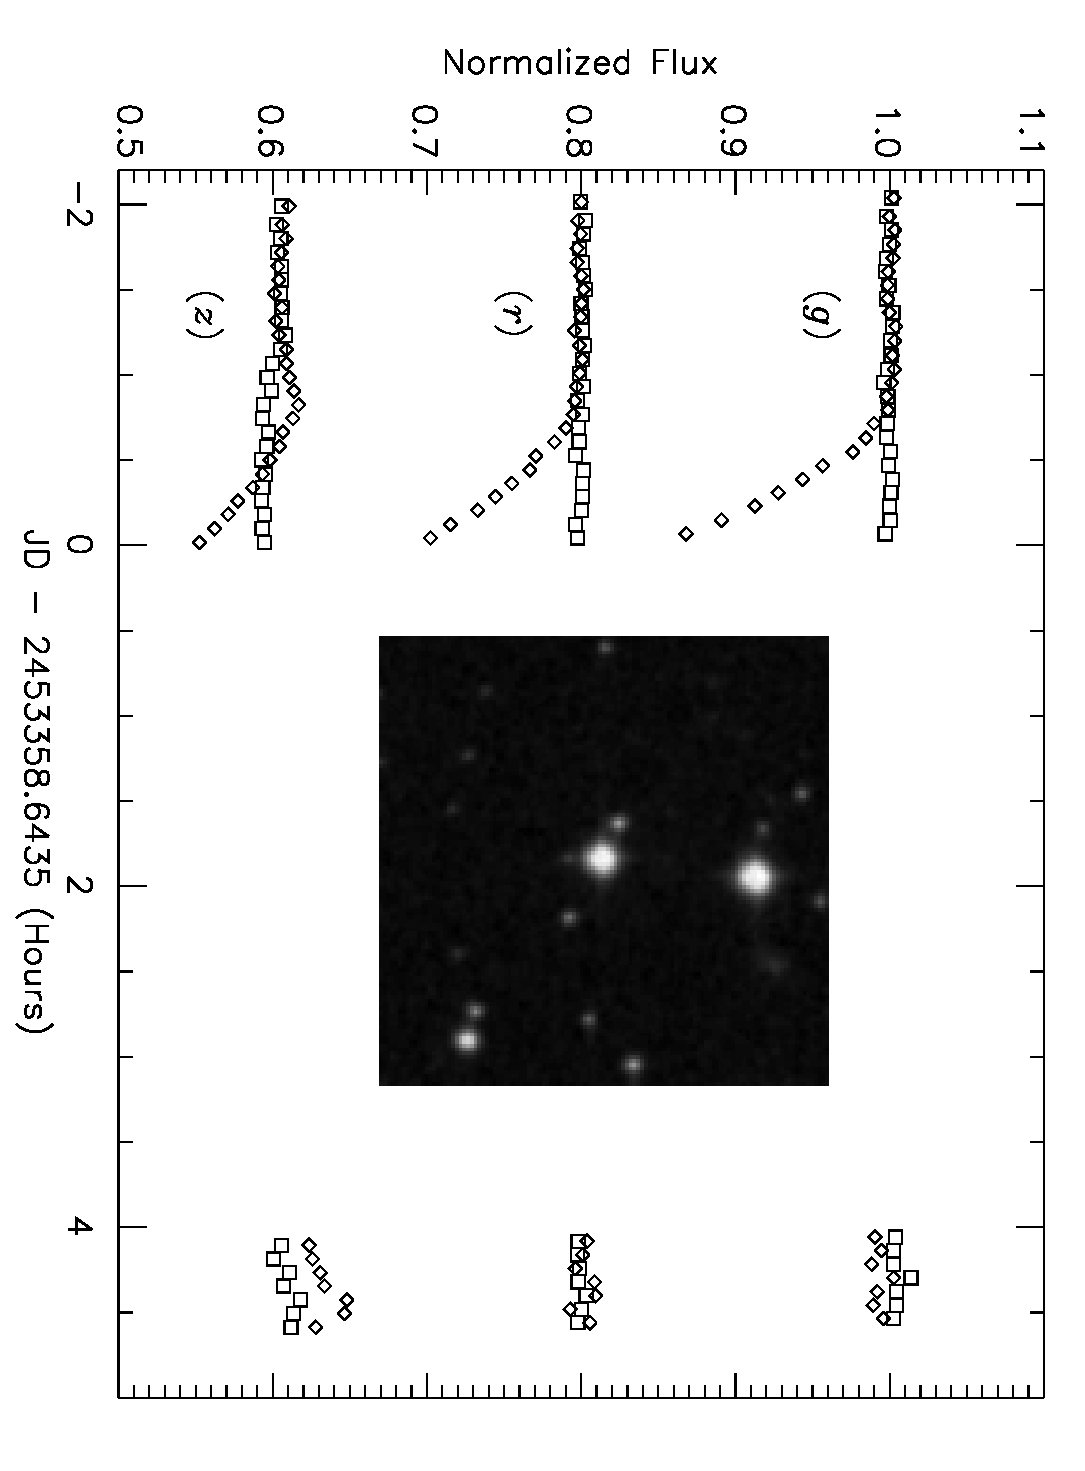
\includegraphics[angle=90, width=0.95\textwidth]{2_f6}
\caption[Follow-up photometry of \mbox{T-And0-03874}, a blended eclipsing binary]{
Follow-up $g$-, $r$-, and $z$-band photometry with the FLWO 1.2-meter telescope of \mbox{T-And0-03874} (\textit{squares}) and a neighboring star (\textit{diamonds}), designated \mbox{T-And0-02943}, that lies $45\arcsec$ away. (The inset $2\arcmin \times 2\arcmin$ Digitized Sky Survey image shows \mbox{T-And0-03874} at the center and \mbox{T-And0-02943} above, to the north.) %
The flux from each star has been normalized using the out-of-eclipse data, and an offset  applied for the purpose of plotting. Inclement weather prevented complete coverage of the predicted eclipse event. Nevertheless, it is evident that \mbox{T-And0-02943} displays a deep ($>$14\%) eclipse, whereas the flux from \mbox{T-And0-03874} is constant. The observed apparent transits of \mbox{T-And0-03874} were the result of the blending of the light from these two systems. With a FWHM for \mbox{T-And0-02943} of $\sim$2.5\,pixels ($\sim$25$\arcsec$), some of the light from this star was within the photometric aperture radius ($3$\,pixels; $\sim$30$\arcsec$) of \mbox{T-And0-03874}.}\label{cha:and0:fig:blend}
\end{center}
\end{figure}

\begin{figure}
\begin{center}
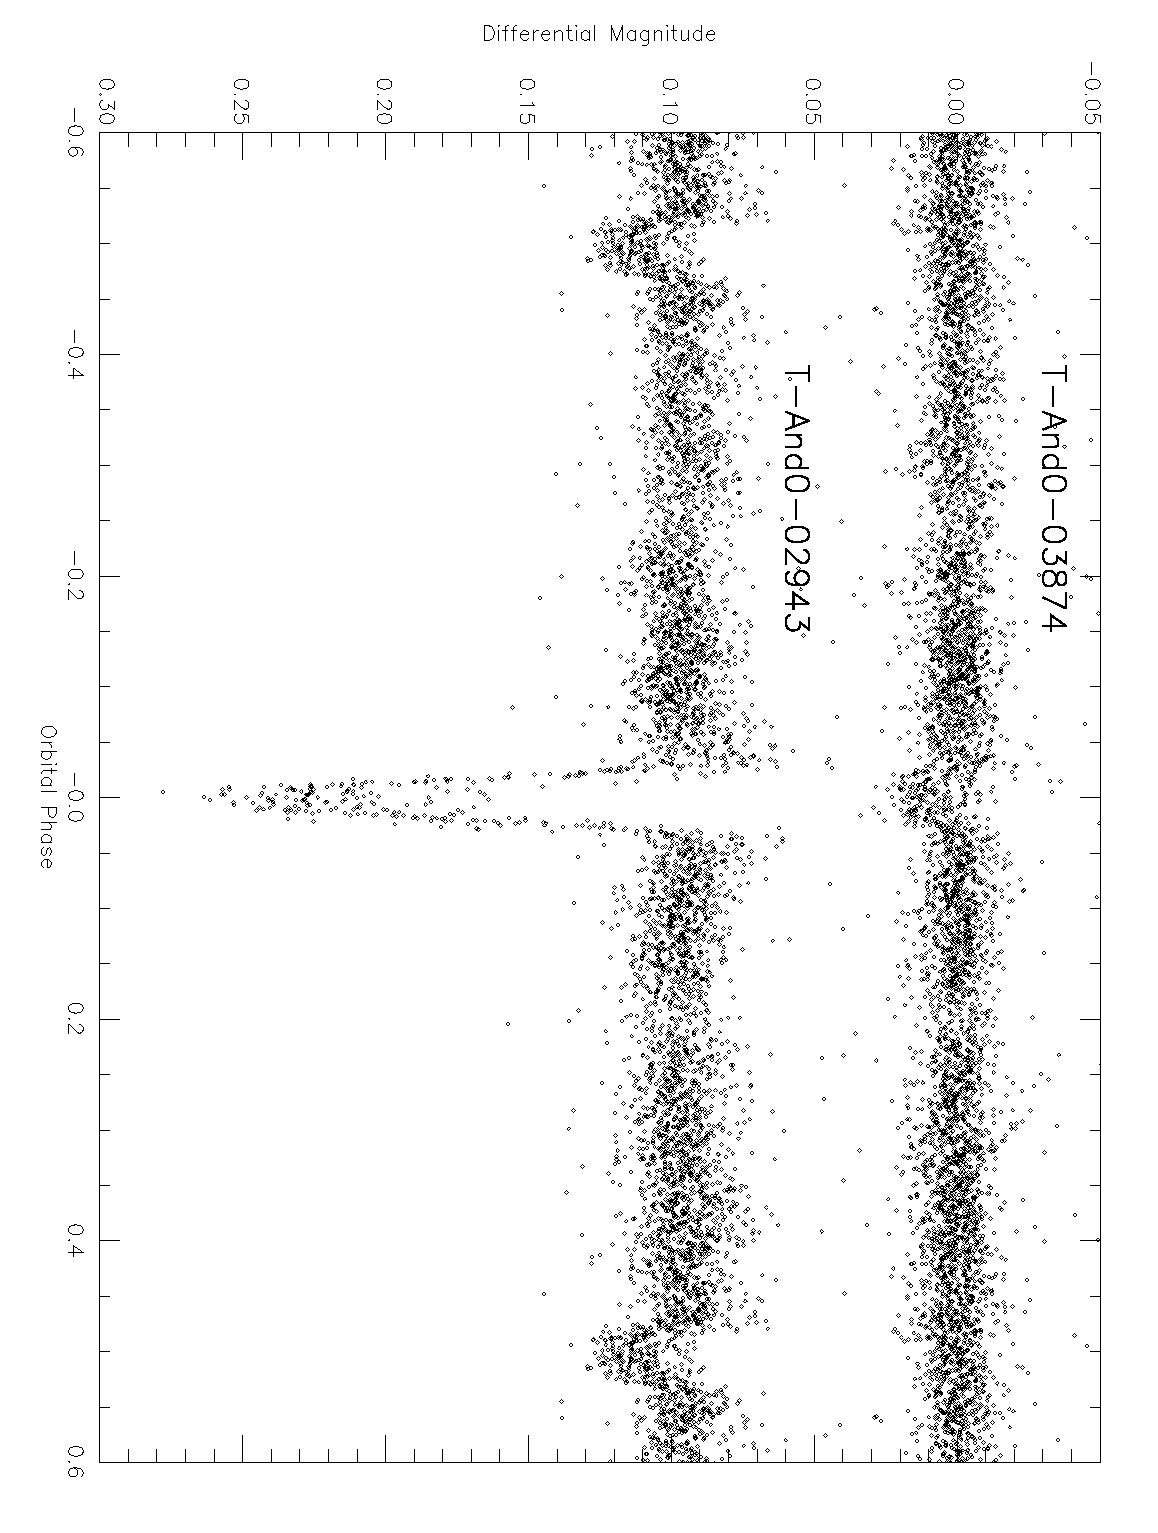
\includegraphics[angle=90, width=0.95\textwidth]{2_f7}
\caption[TrES photometry of \mbox{T-And0-03874} and the neighboring binary]{TrES photometry of \mbox{T-And0-03874} and the neighboring eclipsing binary \mbox{T-And0-02943}, phased to the best-fit period (2.6540\,days) for \mbox{T-And0-03874} derived by the box-fitting algorithm. Both stars show eclipses with the same orbital period and epoch. The $\sim$1\% transit-like event detected in the light curve of \mbox{T-And0-03874} was the result of the blending of light from this star and from \mbox{T-And0-02943}, which lies $45\arcsec$ away, comparable to the $30\arcsec$ radius of the TrES PSF. }\label{cha:and0:fig:compblend}
\end{center}
\end{figure}

The red color of \tFive\ ($J-K_{s}=0.66$\,mag) and the effective temperature ($T_{\mathrm{eff}}=5500$\,K) calculated from the spectrum shown in figure~\ref{cha:and0:fig:spectra}$e$ are consistent with an early K-type star. The radial velocity of \tFive\ was observed to remain constant at $-15.53\,\mathrm{km\,s^{-1}}$. However, the low estimated surface gravity ($\log{g}=3.5$) suggested this star is a giant star and part of a diluted triple. The photometric follow-up (see figure~\ref{cha:and0:fig:blend}) failed to recover transits of \tFive, but did observe a nearby eclipsing binary \mbox{T-And0-02943} undergoing a deep eclipse at the predicted transit time (also shown in figure~\ref{cha:and0:fig:blend}). When we examined our TrES observations for \mbox{T-And0-02943}, we saw that the period of this eclipsing binary was that originally derived for \tFive, namely 2.654 days. This eclipsing system lies $45\arcsec$ away from \tFive, comparable to the PSF radius of our TrES aperture photometry ($30\arcsec$; 3 pixels). The angular resolution ($\sim$1$\arcsec\,\mathrm{pixel}^{-1}$) of the 1.2-meter photometry is higher than that of the original TrES photometry ($9.9\arcsec\,\mathrm{pixel}^{-1}$); hence the light from these two systems is blended in our TrES observations (see figure~\ref{cha:and0:fig:compblend}) but is resolved in the 1.2-meter photometry.

Finally, the observed parameters for \tSix\ ($\log{g}=3.5$, $T_{\mathrm{eff}}=7750$\,K, $J-K_{s}=0.25$\,mag) again imply a large stellar radius ($R\sim1.8\,R_{\sun}$). In order to produce the 0.9\% transit, a companion radius of $1.5\,R_{\mathrm{Jup}}$ is required. This is consistent with the large radii of the transiting planets
 \hatponeb\ \citep{Bakos_Noyes_Kovacs:apj:2007a}, and \wasponeb\ \citep{Charbonneau_Winn_Everett:apj:2007a},
although we have not ruled out the possibility of a blend. Regardless, the star \tSix\ is rapidly rotating ($v\sin{i}=88\,\mathrm{km\,s^{-1}}$; see figure~\ref{cha:and0:fig:spectra}$f$), making precise radial-velocity follow-up extremely difficult.

%\section{Discussion}
\section{Maximizing the Yield from TrES}\label{cha:and0:sec:discuss}

The Trans-atlantic Exoplanet Survey monitors $\sim$30,000 stars each year from which we identify $\sim$30 stars whose light curves show periodic eclipses consistent with the passage of a Jupiter-sized planet in front of a Sun-like star. In order to eliminate astrophysical false positives, we have established a procedure of multi-epoch photometric and moderate-precision spectroscopic follow-up. Surviving candidates are optimal targets for high-precision multi-epoch radial velocity measurements that will yield the masses of planetary companions.

The TrES field in Andromeda was one of the first of our fields for which we combined the data from the three TrES telescopes. We have demonstrated here the benefit of this: the improved transit visibility, the increase in number of stars with low rms residual, and the confirmation of transit events observed by different telescopes. It has also provided us with several examples of the astrophysical false positives that will be encountered in any ground-based, wide-field transit survey, all of which were rejected as a result of follow-up observations. Based on our experience with these false positives, we refined the criteria by which we identify TrES planet candidates. For each new transit candidate, we now search our data set for a nearby eclipsing binary with a similar period as derived by the BLS algorithm in order to check for blends. We also examine the transit light curve phased using integer multiples or fractions of the BLS orbital period.

In comparison to other, more subtle examples (such as those discussed by \citealp{ODonovan_Charbonneau_Torres:apj:2006a} [see chapter~\ref{cha:gsc}], \citealp{Torres_Konacki_Sasselov:apj:2004b}, and Mandushev et al., \citeyear{Mandushev_Torres_Latham:apj:2005a}), these transit candidates were easily identified as false positives.
These examples demonstrate the need for both spectroscopic and photometric follow-up of transit candidates, which may be accomplished with the one-meter class telescopes, on which time is readily available. This ensures that the precious resource of ten-meter spectroscopy is used efficiently.


% chktex-file 44 chktex-file 15
\chapter[Rejecting Astrophysical False Positives from the TrES Transiting Planet Survey: The Example of \mbox{GSC 03885-00829}]{Rejecting Astrophysical False Positives from the TrES Transiting Planet Survey: The Example of \mbox{GSC 03885-00829}%
\protect\CFNA%
}\label{cha:gsc}

\section*{Abstract}\label{cha:gsc:sec:abs}
\addcontentsline{toc}{section}{Abstract}

  Ground-based wide-field surveys for nearby transiting gas giants
  are yielding far fewer true planets than astrophysical false
  positives, some of which are difficult to reject. Recent experience
  has highlighted the need for careful analysis to eliminate
  astronomical systems in which light from a faint eclipsing binary is
  blended with that from a bright star. During the course of the
  Trans-atlantic Exoplanet Survey, we identified a system presenting
  a transit-like periodic signal. We obtained the proper motion and
  infrared color of this target (\gscOTE) from publicly available
  catalogs, which suggested this star is an F dwarf, supporting our
  transit hypothesis.  This spectral classification was confirmed
  using spectroscopic observations from which we determined the
  stellar radial velocity. The star did not exhibit any signs of a
  stellar mass companion. However, subsequent multicolor photometry
  displayed a color-dependent transit depth, indicating that a blend
  was the likely source of the eclipse. We successfully modeled our
  initial photometric observations of \gscOTE\ as the light from a K-dwarf binary system superimposed on the light from a late F-dwarf
  star. High-dispersion spectroscopy confirmed the presence of light
  from a cool stellar photosphere in the spectrum of this system. With
  this candidate, we demonstrate both the difficulty in identifying
  certain types of false positives in a list of candidate transiting
  planets and our procedure for rejecting these imposters, which may
  be useful to other groups performing wide-field transit surveys.

\section{Transits versus Blended Eclipses}\label{cha:gsc:sec:intro}

The discovery of the $169$ known extrasolar planets%
\footnote{Updates available from the
Extrasolar Planets Encyclopaedia:\\
\url{http://www.obspm.fr/planets/}\ .}%
\ has greatly enhanced our
understanding of planetary systems. Most of these extrasolar planets
have been identified from Doppler surveys that search for the radial
velocity variation of a star caused by the presence of a gas giant.
These observations can estimate the period and eccentricity of the
planetary orbit, and provide a lower limit for the planetary mass
relative to that of the star. Assuming that the stellar mass can be
precisely determined, perhaps by comparing the stellar spectra to
stellar atmosphere models (\citealp[such as][]{Kurucz:ATLAS9:1993a}),
the minimum mass of the planet can be derived.  The diversity of these
planetary systems has drastically altered our theoretical appreciation
of their morphology and evolution, including the existence of ``hot
Jupiters'', Jupiter-sized planets with periods of a few days that
experience high insolation from the nearby star.  However, less is
known about the nature of the planets themselves, except for the cases
when a hot Jupiter was observed to pass in front of a dwarf star. By
observing such a transit (as was first suggested by
\citealt{Struve:obs:1952a}), we can estimate the radius of the
transiting planet from the fraction of starlight the planet blocks
during the transit and the radius of the star itself, which must be
measured from stellar model fits to spectra of the star. For a transit
to occur, the planetary orbital inclination must be approximately
$90\degr$; this implies that the Doppler limit for the planetary
mass must be close to the actual mass of the planet. At the
time of writing, we have estimates for the radii and masses of 9 planets from transit
observations similar to those first successfully performed by
\citet{Charbonneau_Brown_Latham:apjl:2000a} and
\citet{Henry_Marcy_Butler:apj:2000a}. These estimates provide
constraints for the competing theories of planetary formation. For
example, the recently discovered transiting ``hot Saturn''
\mbox{HD\,149026\,b} has a mass and radius that imply the
planet has a large core (approximately $70\,\mathrm{M}_{\earth}$;
\citealt{Sato_Fischer_Henry:apj:2005a, Charbonneau_Winn_Latham:apj:2006a}).
It is hypothesized that this planet must have formed via core
accretion \citep{Pollack:araa:1984a, Pollack_Hubickyj_Bodenheimer:icarus:1996a},
rather than through gravitational instability \citep{Boss:sc:1997a}.
However, not every observation of a transiting planet can be explained
by current models of close-in giant planets experiencing high stellar
insolation. The transiting planet \hdTZNb\ has a radius larger than
other planets of its mass and larger than the predicted radii
(\citealp[see][ and references
therein]{Laughlin_Wolf_Vanmunster:apj:2005a};
\citealt{Deming_Seager_Richardson:nat:2005a}).

Several wide-field photometric surveys with the goal of identifying
nearby transiting planets are currently active. Our
Trans-atlantic Exoplanet Survey%
\footnote{See \url{http://www.astro.caltech.edu/\~ftod/tres/}\ .}%
\ (TrES) is a network of three ten-centimeter telescopes:
Sleuth (located at Palomar Observatory, California; \citealt{ODonovan_Charbonneau_Kotredes:AIP:2004a}), the Planet Search Survey Telescope (PSST, Lowell Observatory, Arizona; \citealt{Dunham_Mandushev_Taylor:pasp:2004a}),
and the STellar Astrophysics and Research on Exoplanets%
\footnote{See \url{http://www.hao.ucar.edu/public/research/stare/stare.html}\ .}%
\ telescope (STARE, Tenerife, Spain; \citealt{Alonso_Deeg_Brown:an:2004a}). The TrES
campaign, together with other wide-field surveys such as the HAT
network \citep{Bakos_Lazar_Papp:pasp:2002a} and SuperWASP
\citep{Street_Pollaco_Fitzsimmons:ASP:2003a}, are monitoring thousands
of nearby bright stars ($9\leq V \leq 13$). We hope to find recurring
eclipses with the short period and small amplitude corresponding to a
transiting hot Jupiter. The brightness of the target stars facilitates
both the photometric precision and the follow-up of any identified
transiting planets using space-borne telescopes. Examples of detailed
follow-up observations include the measurement of several chemical
abundances in the atmosphere of \hdTZNb\
\citep{Charbonneau_Brown_Noyes:apj:2002a, Vidal-Madjar_Lecavelier-des-Etangs_Desert:nat:2003a}
and the first direct detections of emitted planetary radiation
\citep{Charbonneau_Allen_Megeath:apj:2005a, Deming_Seager_Richardson:nat:2005a}.

Many astrophysical systems exist that mimic the light curve of a
transiting hot Jupiter. Due to the mass-radius degeneracy for bodies
with masses between 0.001 and 0.1\,\msun, the depth of an eclipse
of a solar-type star by a hot Jupiter, a brown dwarf or an M dwarf
star will be about 1\% in each case, despite the large range in mass.
Grazing incidence eclipsing binaries may also exhibit comparable
eclipse depths. For wide-field ground-based surveys, the frequency
of the false positives is greater than the frequency of detection of
true transiting planets, by at least an order of magnitude.  As part
of TrES, we typically identify 10--20 of these transit-like
photometric signals out of 15,000--25,000 stars ($10<V<15$) in each
$6\degr \times 6\degr$ target field of view ($b\sim15\degr$; %
\citealp[see, e.g.,][]{Dunham_Mandushev_Taylor:pasp:2004a}), and
similar yields should be expected from other wide-field ground-based
surveys. This number (which is dependent on the density of star
counts, and hence the Galactic latitude) is consistent with
theoretical predictions. For example, \citet{Brown:apjl:2003a} predicts
that for every 25,000 stars observed, we will find 10 false positives
and only one true transiting planet. This assumes that we must observe three transit events for each candidate and is dependent on the
visibility of transits throughout the observation run. The low yield
of planets necessitates a rigorous routine of follow-up observations
and detailed analysis to eliminate all possible alternatives to the
planet hypothesis. One straightforward method to reduce the number of
false positives is to obtain multi-epoch spectroscopy of each
candidate and measure radial velocities with a precision of $\sim$1\,$\mathrm{km\,s^{-1}}$. From this we can identify targets with
companions of stellar, rather than planetary, mass (%
\citealp[see,
e.g.,][]{Latham:ASP:2003a, Charbonneau_Brown_Dunham:AIP:2004a}). We can
also estimate the luminosity class of the target star to single out
and reject giants.

The blending of the light from an edge-on binary system with that
from a third star can also be mistaken for a transit.
\citet{Brown:apjl:2003a} predicts that half of the false positives from
a typical wide-field survey will be of this type; the other half will
be grazing eclipsing binaries. Blends can be much more difficult to
identify. The faintness of the binary compared to the third star can
prevent the detection of the radial velocity variations of the
binary. These variations are also masked by the rotationally broadened
spectral lines of the rotationally synchronized binary stars. However,
if the binary has a significant difference in effective temperature
from that of the third star, the eclipse depths should display a
strong color dependence, unlike the color-independent transits of a
(dark) planet across a single star.  Nevertheless, there has been
recent experience of blends with color-independent eclipse depths. In
the case of \ogletrTT\ \citep{Torres_Konacki_Sasselov:apj:2004b} and \gscOON\ \citep{Mandushev_Torres_Latham:apj:2005a}, both candidates (a
suspected planet and brown dwarf, respectively) showed
color-independent eclipse depths, and yet were subsequently
discovered to be blended systems. Evidence for the presence of an
eclipsing binary was found from a careful analysis of the spectral
line shapes, prompting the authors to compare the photometric data to
simulations of blends. \ogletrTT\ was shown to
be a hierarchical triple consisting of a bright F6 dwarf and an
F4+(K7--M0) binary.
The blend model for \gscOON\ comprises an F5 primary and a G0+M3
binary. In both cases, the similarity in color between the primary
star and the brightest member of the binary explains the constant
eclipse depth at different wavelengths. The high occurrence of such
false positives and the difficulty in rejecting them requires a
detailed study of candidates before any announcement is made, as was
done in the case of \tresOne\
\citep{Alonso_Brown_Torres:apjl:2004a} and \ogletrFSb\ \citep{Torres_Konacki_Sasselov:apj:2004a}.

Here we discuss a promising candidate, \gscOTE, from one of our target
fields. Initial photometric (section~\ref{cha:gsc:sec:tres}) and spectroscopic
(section~\ref{cha:gsc:sec:spec}) monitoring of this candidate strongly suggested
that we were observing a Saturn-sized companion transiting a solar
type star every 1.441 days with a transit depth of approximately
6\,mmag. However, follow-up photometry (section~\ref{cha:gsc:sec:photo}) displayed
a slight color dependence as might be caused by a blend, and we were
able to model our photometry using simulations of blended eclipsing
binaries (section~ref{cha:gsc:sec:blend}). Our best-fit model consists of a bright
F dwarf and a K-dwarf binary, and we were able to identify the presence
of light from the binary in the spectrum of \gscOTE\ (section~\ref{cha:gsc:sec:nirspec}).
The faintness of the binary system
prevents us from identifying the presence of asymmetric spectral
lines, as was done by \citet{Torres_Konacki_Sasselov:apj:2004b} and
\citet{Mandushev_Torres_Latham:apj:2005a}. In this case, only
multicolor observations provided us with the necessary evidence to
call into question the planetary nature of this candidate.

\section{TrES Telescope Observations of \\ \mbox{GSC 03885-00829}}\label{cha:gsc:sec:tres}

In 2004~March, we commenced observations of a $6\degr\times6\degr$
target field in Draco. The field is centered on our $V=4.8$ guide star
\mbox{HD\,151613} (\mbox{$\alpha = 16^{\rm h} 45^{\rm m}
17.82^{\rm s}$}, \mbox{$\delta = +56\degr 46\arcmin 54.7\arcsec$} J2000.0). Between
UT 2004 March~29 and June~22, we observed this field nightly with
Sleuth at Palomar Observatory (California) and with PSST at Lowell
Observatory (Arizona). STARE, in Tenerife (Spain), did not observe
this field as it was undergoing repairs at this time. A total of $15,\!854$
photometric exposures of 90\,s each were obtained through either a
Sloan $r$ filter (Sleuth) or a Kron-Cousins $R$ filter (PSST).

We bias-subtracted and flat-fielded the images of our target field
once the data were transferred from the observatory computers. We
performed the calibration of the Sleuth data using customized IDL
routines; we calibrated the PSST data using the \texttt{zerocombine},
\texttt{ccdproc}, and \texttt{flatcombine} tasks in the IRAF%
\footnote{IRAF is distributed by the National Optical Astronomy
  Observatories, which are operated by the Association of Universities
  for Research in Astronomy Inc. under cooperative agreement with
  the National Science Foundation.}%
\ package \citep{Tody:1993a}. We reduced the Sleuth and PSST
photometric data separately as follows using our difference image
analysis (DIA) pipeline (%
\citealp[described in][]{Dunham_Mandushev_Taylor:pasp:2004a},
\citealp[and based in part on][]{Alard:aas:2000a}).

We created our reference image for the field from images obtained at
low air mass on a photometric night during dark time. We obtained a
standard list of stars from this image using profile-fitting (point-spread function, PSF)
photometry (\mbox{DAOPHOT II}/ALLSTAR;
\citealt{Stetson:pasp:1987a, Stetson:ASP:1992a}). We calculated the
equatorial coordinates ($\alpha,\delta$) of these stars by matching a
subset with the stars listed in the Tycho-2 Catalog
\citep{Hog_Fabricius_Makarov:aa:2000a} and then spatially
interpolated all of the science images so that the star coordinates
from each image matched those from our standard star list.

We produced the master image for the Sleuth data set by combining 19
of our best-quality interpolated images; we combined 17 images to
create the corresponding PSST master image. We subtracted each
interpolated image from this master image. We used aperture photometry
on the resultant difference images (using the centroids derived for
the standard star list) to estimate the flux of each star in each
image. We produced time series consisting of the differences between
the magnitude of a star in the reference image and the magnitude of
that star in each target image in turn. We decorrelated these light
curves as follows to remove systematic effects typical of wide-field
surveys, such as those caused by changing atmospheric conditions
throughout the night. We listed the stars in order of brightness, and
divided the list into batches of 500. We computed the least-squares
fit to the light curve of a given star from a linear combination of
the other light curves in that batch. We then subtracted this
least-squares fit from the light curve of the star.

In our previous studies
(\citealp{Alonso_Brown_Torres:apjl:2004a}; \citealp{Mandushev_Torres_Latham:apj:2005a}; \citealp{Creevey_Benedict_Brown:apjl:2005a}),
we presented separate light curves from one of the TrES telescopes.
For this field, we combined the two data sets. For a given star on the
Sleuth standard star list, we calculated the angular distances between
that star and the PSST standard stars. We matched the Sleuth star with
a PSST star if the angular distance was less than $5\arcsec$ (0.5
pixels). Due to the difference in the selected filter and the
telescope pointing between the two sites, some stars were unique to a
given standard star list, and no match was found. We appended the time
series for each matched PSST star to the corresponding Sleuth time
series, and reordered the combined time series chronologically. The
data for the unmatched PSST stars were simply added to the resulting
data set.

In order to reduce the computational intensity of our transit search,
we averaged the combined time series in 9-minute-wide bins to obtain
2996 binned observations. Since central transits should last 3\,hr (see section~\ref{cha:intro:sec:methods:sub:trans}),
this did not significantly sacrifice temporal resolution of potential
transit events. For $\sim$10,000 stars, the rms scatter of the binned
data was below 0.04 mag. We performed a search of the time series of
these stars using the box-fitting least-squares (BLS) transit-search
algorithm (Kovacs, Zucker, \& Mazeh~\citeyear{Kovacs_Zucker_Mazeh:aa:2002a}, see appendix~\ref{cha:bls}) to identify periodic transit events. The BLS algorithm calculates a Signal
Detection Efficiency (SDE;
\citealp[see][]{Kovacs_Zucker_Mazeh:aa:2002a}) for each candidate,
which denotes how significant the detection is. We identified
candidates based on this SDE, followed by a visual inspection.

\begin{figure}
\begin{center}
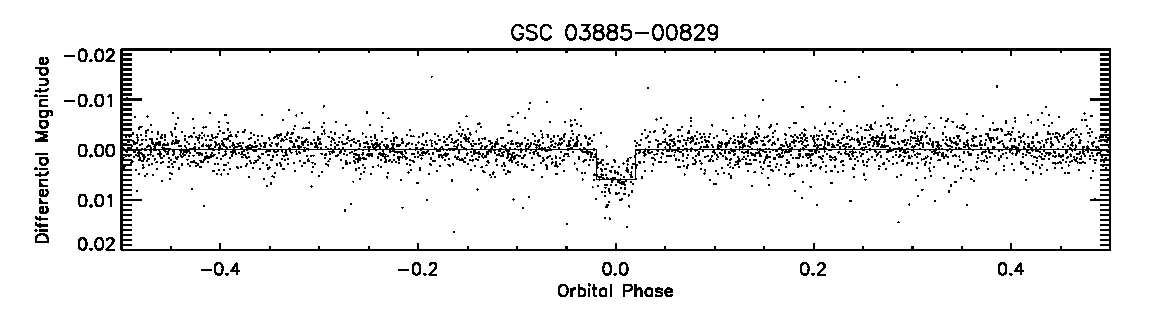
\includegraphics[width=0.95\textwidth]{3_f1}
\caption[TrES light curve of \mbox{GSC 03885-00829}, a blended eclipsing binary]{Binned TrES $r$-band light curve of \mbox{GSC 03885-00829},
  folded with the photometric period of 1.441 days computed using the
  box-fitting least-squares algorithm. Overlaid is the corresponding
  box transit model.}\label{cha:gsc:fig:discovery}
\end{center}
\end{figure}

Many of the candidates identified for this field show V-shaped
eclipse, a possible ellipsoidal variability, or have large depths,
making it likely that they are not transiting planets, but rather
eclipsing binaries.  However, we promptly identified a promising
candidate. When the data for this star were folded with the
photometric orbital period of 1.441 days (calculated using the BLS
algorithm), the resultant light curve (figure~\ref{cha:gsc:fig:discovery})
displayed a shallow and flat-bottomed transit, and no noticeable
ellipsoidal variability out of transit. The depth ($\sim$6\,mmag) and
duration (1.4\,hr) of the occultation are consistent with a
Saturn-sized planet transiting a solar-type star.  The SDE for this
candidate ($\sim$20) was high relative to that calculated for typical
TrES candidates ($\sim$10--15).

\begin{deluxetable}{lc}
\tablewidth{0pt}
\tablecaption{Data for \mbox{GSC 03885-00829}\label{cha:gsc:tab:gsc}}
\tablehead{\colhead{Parameter} & \colhead{Value} }
\startdata
R.A. \phm{000..} (J2000.0)    & \phm{000} \phn \phs $16^{\rm h} 52^{\rm m} 33.7^{\rm s}$ \\
Decl. \phm{000.} (J2000.0)  & \phm{000} $+57\degr 58\arcmin 27\arcsec$ \\
GSC & \phm{00000} \phn 03885-00829 \\
2MASS & \phm{00000} 16523368+5758262 \\
 & \\
$V$ \tablenotemark{a} \phm{$-R_{\rm C}$0.} (mag) & \phm{0000.} $10.465 \pm 0.001$ \\
$B-V$  \tablenotemark{a} \phm{0.} (mag) & \phm{00000.} $0.612 \pm 0.001$ \\
$V-R_{\rm C}$  \tablenotemark{a} \phm{.} (mag) & \phm{0000.} \phn$0.371 \pm 0.003$ \\
$V-I_{\rm C}$  \tablenotemark{a} \phm{0} (mag) & \phm{0000.} \phn$0.743 \pm 0.001$ \\
$J$  \tablenotemark{b} \phm{$-R_{\rm C}.$0} (mag) & \phm{0000.} \phn$9.197 \pm 0.018$ \\
$J-H$  \tablenotemark{b} \phm{0.} (mag) & \phm{000000}$0.337 \pm 0.023$ \\
$J-K_{s}$  \tablenotemark{b} \phm{0} (mag) & \phm{0000.} \phn$0.440 \pm 0.026$ \\
& \\
Period \tablenotemark{c} \phm{.0} (days) & \phm{00000.} $2.88244 \pm 0.00046$ \\
$T_{2}$ \tablenotemark{d} \phm{0000..} (HJD) & $2453529.833 \pm 0.009$ \\
Depth \phm{00.} ($r$ mag) & \phm{00000.} $0.006 \pm  0.003 $
\enddata
\tablenotetext{a}{See section~\ref{cha:gsc:sec:photo} for a discussion of errors.}
\tablenotetext{b}{From the 2MASS Catalog \citep{Cutri_Skrutskie_van-Dyk:2003a}.}
\tablenotetext{c}{The period of the suspected candidate planet was $1\fd44122 \pm 0\fd00023$.}
\tablenotetext{d}{The time of the \textit{secondary} eclipse of the binary, and the central transit time of the candidate.}
\end{deluxetable}

Supporting data from online catalogs provided further evidence of the
planetary nature of this eclipse. Using the SIMBAD%
\footnote{See \url{http://simbad.harvard.edu/}\ .}%
\ database, we identified our candidate as the star \gscOTE\ (see
table~\ref{cha:gsc:tab:gsc}). The infrared colors (2MASS $J-K_{s}$, $J-H$;
\citealt{Cutri_Skrutskie_van-Dyk:2003a}) and optical ($B-V$)
colors of this star are near-solar, roughly consistent with the
stellar parameters inferred from our transit observations. This star
displays significant proper motion (26\,mas\,$\mathrm{yr^{-1}}$ from the USNO-B
Catalog; \citealt{Monet_Levine_Canzian:aj:2003a}), suggesting it is a
nearby dwarf. As a first check of the possibility of contamination of
light from a nearby star, we verified that there is no bright star
visible on the Digitized Sky Survey%
\footnote{%
The Digitized Sky Survey (\url{http://archive.stsci.edu/dss/}) was produced at the Space Telescope Science Institute under US Government grant NAG W-2166.
The images of these surveys are based on photographic data obtained using the Oschin Schmidt Telescope on Palomar Mountain and the UK Schmidt Telescope.
The plates were processed into the present compressed digital form with the permission of these institutions.%
}%
\ (DSS) images within our aperture radius ($\leq 30\arcsec$).

With due enthusiasm, we proceeded to obtain follow-up observations of
this exciting candidate, with the goal of rejecting the possibility
that this was not a transiting planet.

\section{Spectroscopic Follow-up of \mbox{GSC 03885-00829}}\label{cha:gsc:sec:spec}

We confirmed that \gscOTE\ was an isolated dwarf star by
spectroscopically monitoring this candidate. We observed \gscOTE,
together with other candidates from this TrES field, with the
Harvard--Smithsonian Center for Astrophysics (CfA) Digital Speedometer
\citep{Latham:ASP:1992a}, operated on the 1.5\,m Tillinghast reflector
at the F.\ L.\ Whipple Observatory (FLWO) on Mount~Hopkins, Arizona.
The spectral coverage was 45\,\AA\ centered on 5187\,\AA\ at a
resolving power of $\lambda / \Delta \lambda \approx 35,\!000$ (a
resolution of $8.5\,\mathrm{km\,s^{-1}}$). We observed this particular
target on UT 2005 May~18, May~20, and May~21, at an orbital phase 0.52,
0.86, and 0.50, respectively (calculated using the orbital ephemeris
of the planet; see table~\ref{cha:gsc:tab:gsc}, footnote~c).

\begin{figure}
\begin{center}
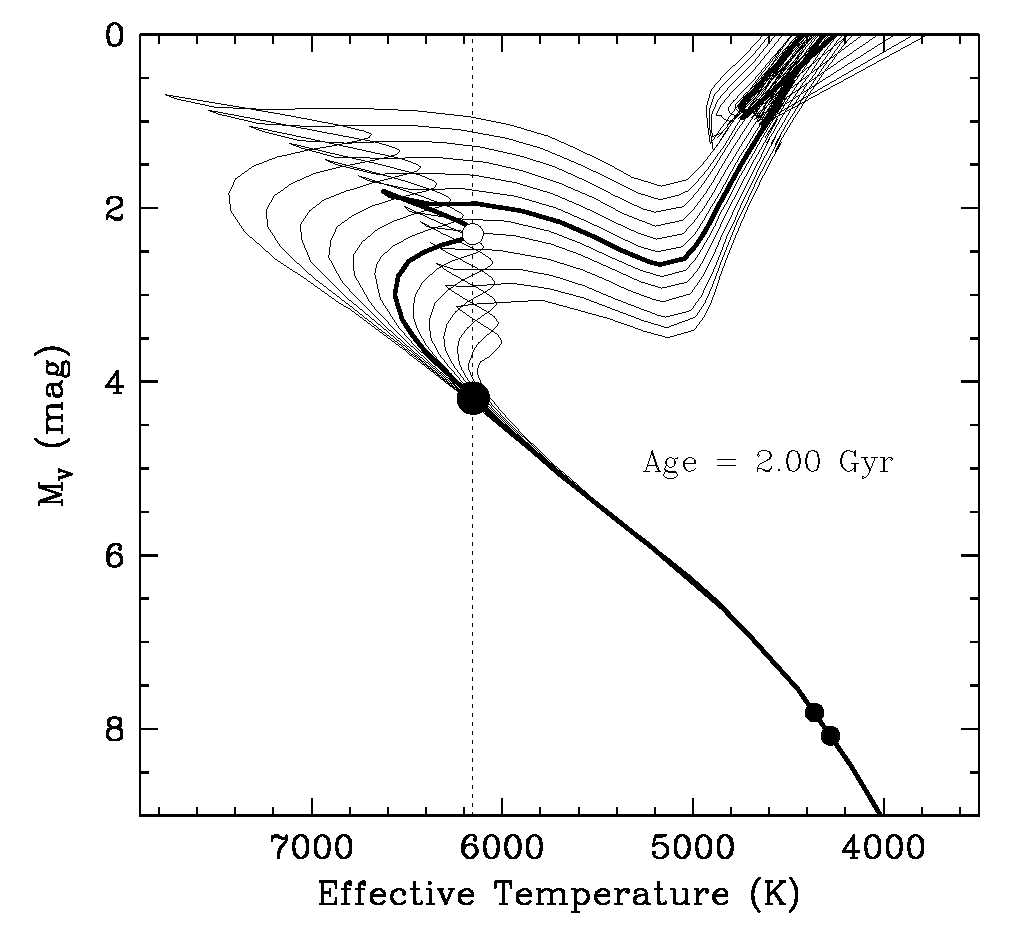
\includegraphics[width=0.95\textwidth]{3_f2}
\caption[Location of blend model components on isochrones]{\citet{Girardi_Bressan_Bertelli:aas:2000a} model isochrones
  for solar metallicity and ages ranging from 1 to 4 Gyr.
  The \textit{open circle} and \textit{large filled circle} represent two main-sequence stars of the same effective temperature as our candidate
  \mbox{GSC 03885-00829} ($T_{\rm eff} = 6150$ K) but different
  degrees of evolution. They are shown on the 2 Gyr isochrone ({\textit thick
  line}), which maximizes the difference in brightness at this
  temperature. The corresponding radii differ by a factor of 2.4. We
  must therefore constrain the evolution of our candidate using
  spectroscopy before we can accurately estimate its radius and hence
  the size of any transiting companion. The three \textit{filled circles} show
  the location of each of the three members of our final blend model
  for this candidate on the 2\,Gyr isochrone. The bright primary has a
  mass of 1.15\,\msun, and the binary component masses are
  0.67 and 0.64\,\msun.}\label{cha:gsc:fig:isochrones}
\end{center}
\end{figure}

\begin{figure}
\begin{center}
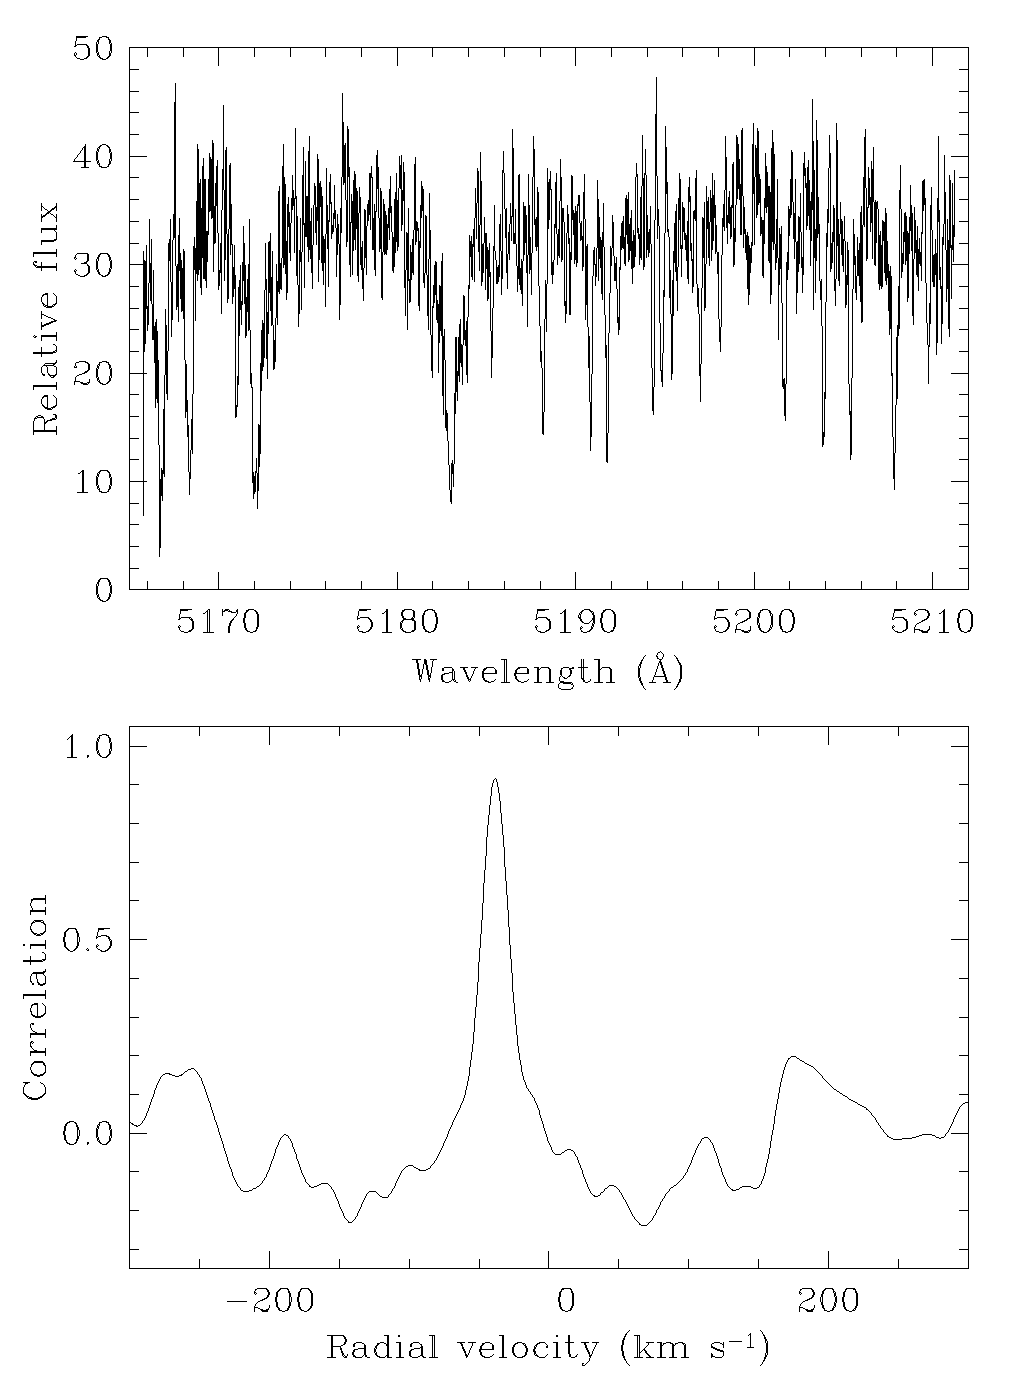
\includegraphics[width=0.95\textwidth]{3_f3}
\caption[Sample spectrum of the F-dwarf \mbox{GSC 03885-00829}]{Sample spectrum of \mbox{GSC 03885-00829} (which includes the
Mg~\textsc{\small I}~$b$ triplet) and the corresponding cross-correlation function.}\label{cha:gsc:fig:spectrum}
\end{center}
\end{figure}

Radial velocities were obtained by cross-correlation using templates
chosen from a library of synthetic spectra computed for us by J.~Morse
and based on the model atmospheres of R.~L.~Kurucz (J.~Morse \&
R.~L.~Kurucz, 2004, private communication; see figure~\ref{cha:gsc:fig:spectrum}). The typical precision of a
single velocity measurement is $0.5\,\mathrm{km\,s^{-1}}$. We measured
the radial velocity to be constant ($-38.48\,\mathrm{km\,s^{-1}}$ with
an rms of $0.28\,\mathrm{km\,s^{-1}}$) within our errors. These
measurements indicate that the target star is not gravitationally
bound to a massive stellar companion. Various stellar parameters were
estimated, again by cross-correlating these spectra against a grid of
templates from our spectral library, seeking the best match.  Assuming
a solar metallicity, we estimated the effective temperature to be
$T_{\mathrm{eff}}=6150$\,K and the surface gravity to be $\log{g}
\approx 4.4$, that suggested this was a late F-dwarf star, consistent
with the proper motion and photometric colors, and with our transit
hypothesis. The formal stellar rotation we derived ($v\sin{i} \approx
1\,\mathrm{km\,s^{-1}}$) is actually below our spectral
resolution. The surface gravity suggests that the star is unevolved. This
constraint is important, as this star lies within the range of
effective temperatures for which an ambiguity exists as to the
corresponding mass of the star while on the main sequence, depending
on the degree of evolution. An illustration of this ambiguity is shown
in figure~\ref{cha:gsc:fig:isochrones}, where the two locations denoted by the
open circle and large filled circle have the same effective
temperature as \gscOTE\ but rather different luminosities. The particular
age of the isochrone for this figure was selected to show this
difference more clearly. The fainter (lower) location corresponds to
an unevolved main-sequence star ($\log{g}=4.34$) of mass
1.15\,\msun, whereas the brighter location is for a star near the
end of the hydrogen-burning phase and has a surface gravity of
$\log{g}=3.68$ and a mass of 1.61\,\msun. The radii differ by a
factor of about 2.4. From this example, we see that, without a surface
gravity constraint, we cannot be sure of the radius of our target
star, preventing our discriminating between a planetary and a stellar
transiting companion.

\section{Photometric Follow-up of \mbox{GSC 03885-00829}}\label{cha:gsc:sec:photo}

Although we had found no evidence of a stellar mass companion from our
radial velocity measurements, the possibility remained that the
observed transits were in fact the eclipses of a faint binary whose
light was blended with that from the bright F dwarf due to the large
pixel sizes of our detectors. Follow-up observations of higher
angular resolution might resolve such a blended system. A possible
wavelength dependence of the eclipse depth from multicolor
observations would also provide evidence of a blend. We organized a
follow-up photometric campaign to observe multiple transits of \gscOTE\
using $D>20\arcsec$ (0.50\,m) telescopes and several different filters.

\begin{figure}
\begin{center}
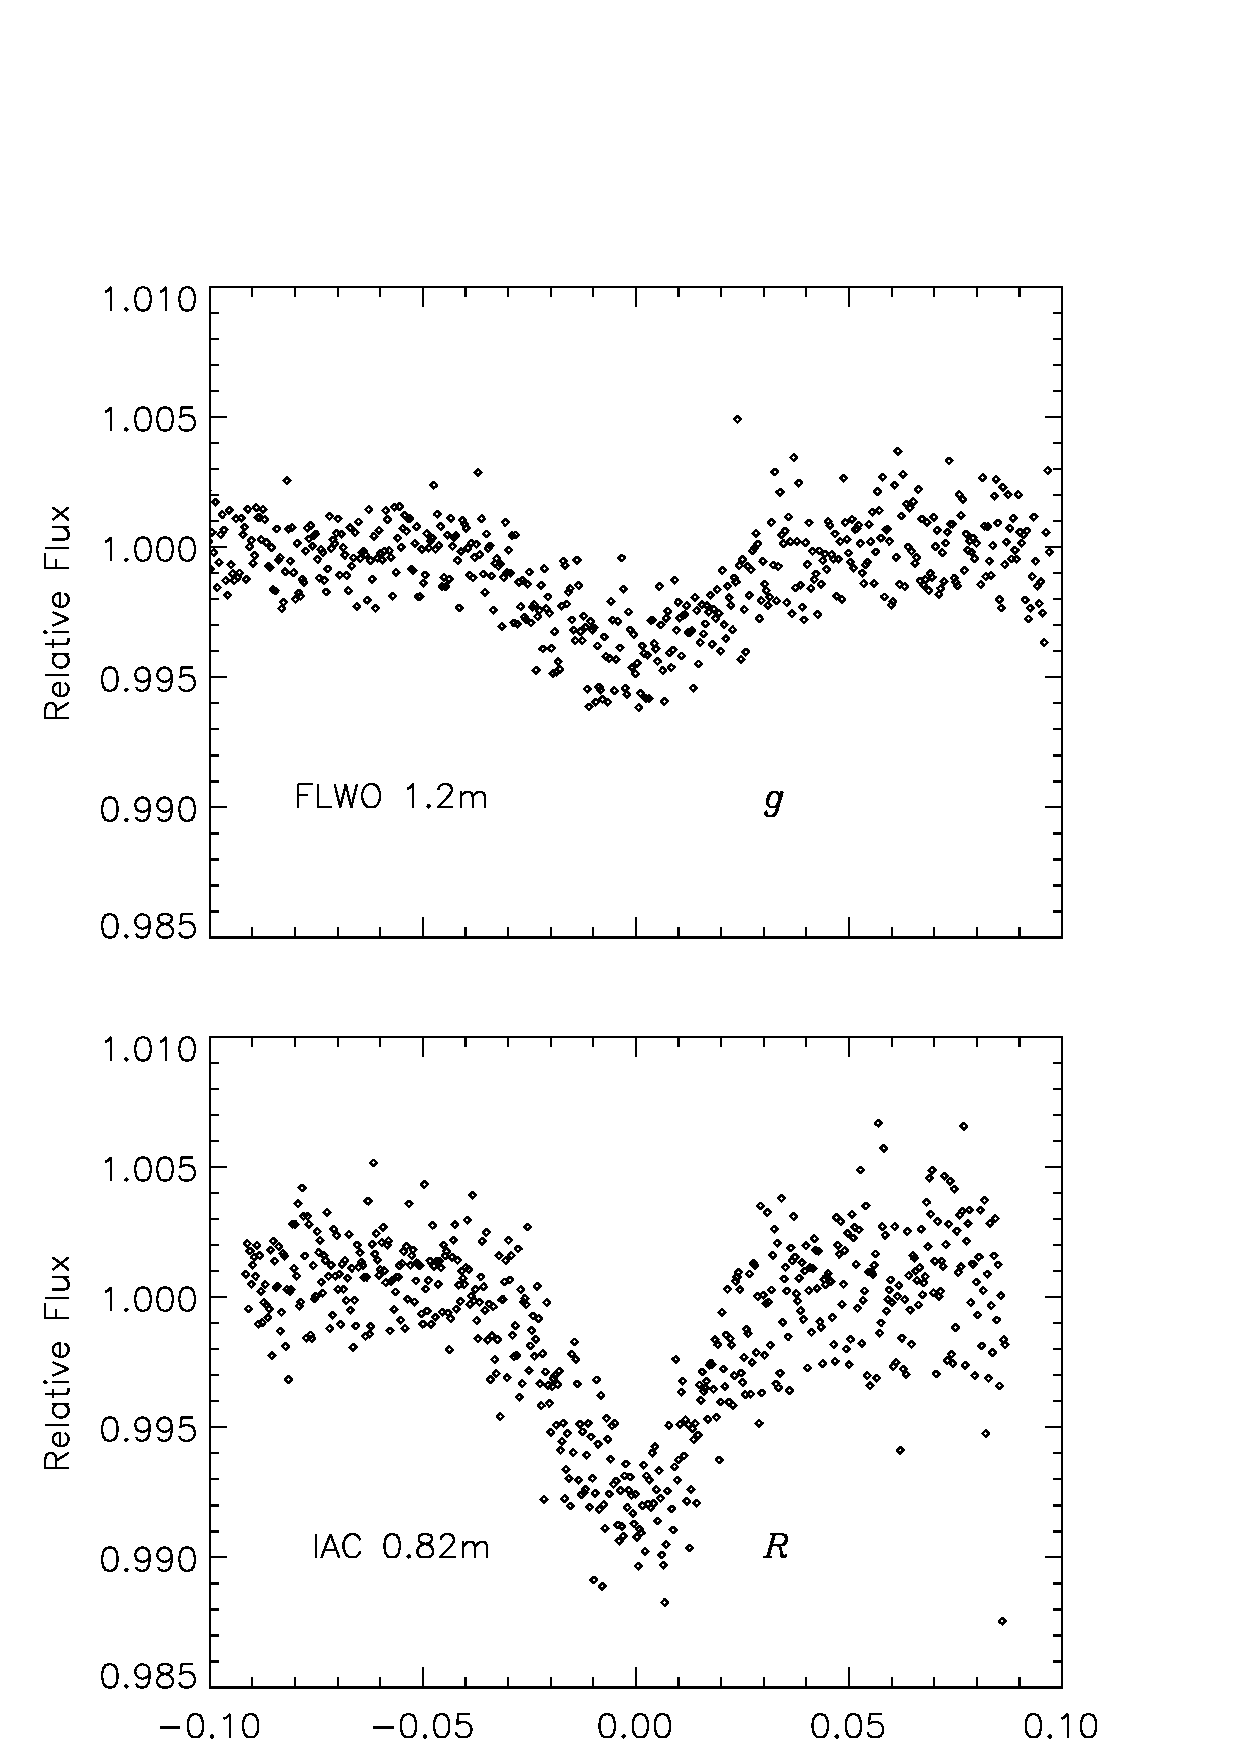
\includegraphics[width=0.95\textwidth]{3_f4}
\caption[Color dependence of recovered transits of \mbox{GSC 03885-00829}]{Our follow-up photometry of \mbox{GSC 03885-00829} near
  the predicted time of transit. The observations were folded using
  the orbital ephemeris of the planet (see table~\ref{cha:gsc:tab:gsc}, footnote~c). Each
  plot is labelled with the corresponding telescope (see text) and
  the filter bandpass. The predicted transit events were observed, but
  an increase in eclipse depth with increasing wavelength is
  apparent.}\label{cha:gsc:fig:multicolor}
\end{center}
\end{figure}

High precision photometry of \gscOTE\ was made on UT 2005 June~8 using
the 1.2\,m FLWO telescope (Arizona).  For this clear, photometric
night, we used MiniCam, a two CCD mosaic, each array being $2048
\times 4608$ pixels.  Observations were binned $2\times2$ for a faster
duty cycle. A Sloan $g$ filter was used, with an exposure time of
30\,s and a corresponding duty cycle of $\sim$50.5\,s.  The telescope
was de-focused to a FWHM of $\sim$15 pixels ($\sim$9$\arcsec$) to
allow greater photon counts per given exposure without saturation.
Spreading the star image also serves to reduce pixel-to-pixel
variations that may not be completely removed by flat-fielding. A
total of 561 photometric measurements of the field were made over a
total of 7.875\,hr. The differential light curve of our target star
was obtained using aperture photometry of this star and one of the
observed reference stars. We corrected for the effect of differential
extinction on the time series by fitting the out-of-eclipse
data. The resultant light curve was then converted to flux units (see
figure~\ref{cha:gsc:fig:multicolor}). These follow-up photometric
observations were made over a year after our TrES images. We used this
separation in time to obtain a more accurate photometric ephemeris for
our candidate, $T_{c} (\mathrm{HJD}) = 2453529.833 + 1.44122 \times E$
(see table~\ref{cha:gsc:tab:gsc}).

\gscOTE\ was observed on the night of UT 2005 June~13 at the 0.82-meter
IAC-80 telescope at the Observatorio del Teide (Tenerife, Spain),
using its $1024 \times 1024$ pixels CCD and a Johnson $R$ filter. To
achieve better photometric precision, a slight defocus was applied, in order to image stars with a FWHM of $\sim$4$\arcsec$.  Exposures times of
22\,s were used, and the readout time using a $2 \times 2$ pixels binning was
$\sim$10\,s. The images were bias and flat-field corrected, and
aperture photometry was applied using the package for optimal aperture
photometry \texttt{vaphot} \citep{Deeg_Doyle:2001a}. Nine reference
stars were used to build an ensemble reference star. The dispersion of
the data points is larger at the end of the night as the star was
closer to the horizon. We corrected for differential extinction;
figure~\ref{cha:gsc:fig:multicolor} shows the derived differential light
curve.

We obtained $BV(RI)_{\rm C}$ observations of \gscOTE\ on UT 2005 June~5
with the Lowell Observatory $42\arcsec$ (1.05-meter) Hall reflector in
combination with a $2048 \times 2048 $ pixels SITe CCD. A total of 223
exposures of the program field were accumulated: four in $B$, 211 in
$V$, three in $R_C$, and five in $I_C$. We observed 20 photometric
standards in the SA107, SA108, SA109, SA112, and PG1633 fields
\citep{Landolt:aj:1992a} in order to calibrate the photometry. We
obtained the following values%
\footnote{The errors include the uncertainties in the Landolt
  photometry and the internal scatter of our photometry, but may not
  account for the total systematic error in the observations.}%
\ for the standard magnitudes of \gscOTE\ (the numbers in the brackets
show the number of individual measurements used to derive the mean
magnitudes): $B = 11.077 \pm 0.001$\,mag (4), $V = 10.465 \pm 0.001$\,mag (12), $R_{\rm C} = 10.094 \pm 0.003$\,mag (3), and $I_{\rm C} = 9.722 \pm 0.001$\,mag (5).

These initial attempts to observe \gscOTE\ convinced us that the target
star displayed a transit-like dip and that nearby stars were not
variable. This reduced the possibility that this signal was caused by
a chance superposition of a star with an eclipsing binary in the large
pixel scale of the TrES detectors. We were also able to reproduce our
$g$-band observations using a model of a Jupiter-sized planet
orbiting a near-solar-type star, although the ingress and egress
appeared to be too long in duration.

It was when we compared the different light curves that we realized
something was wrong with our assumption that these were observations
of a transiting planet. The depth of the transit appeared to vary with
wavelength: an eclipse depth of 0.4\% in the $g$ band and 0.7\% in the
$R$ band. Prompted by the color dependence of the transit depths, we
ran various simulations of the eclipses visible from \gscOTE\ in an
attempt to rule out the possibility of a blend.

\section{Blend Analysis of Observations of \\ \mbox{GSC 03885-00829}}\label{cha:gsc:sec:blend}

\begin{figure}
\begin{center}
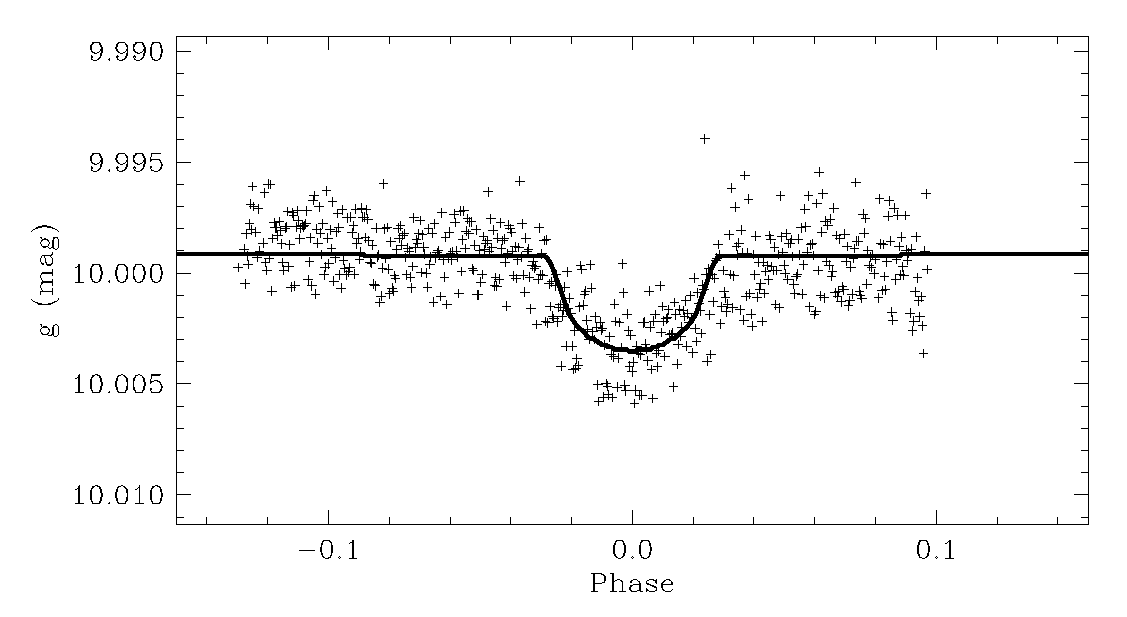
\includegraphics[width=0.95\textwidth]{3_f5}
\caption[$g$-band observations modeled as an F/K+M blend]{Binned $g$-band observations of \mbox{GSC 03885-00829}
  obtained with the FLWO 1.2-meter telescope, folded with the BLS period
  of 1.441 days. Superimposed is the theoretical light curve from a
  blend model consisting of the bright F star and a K+M dwarf
  eclipsing binary (see text). Although the depth of the transit is
  well fit, the predicted duration is slightly shorter than observed.}\label{cha:gsc:fig:KMmodel}
\end{center}
\end{figure}


Light curve fits to the $g$-band observations were carried out as
described in detail by \citet{Torres_Konacki_Sasselov:apj:2004b}.
Briefly, we assumed that the
measured brightness of \gscOTE\ is due to the light of an eclipsing
binary blended with the light of the F star, so that the deep eclipses
of the binary are reduced in depth to the level that we see. We
hypothesized that the three objects formed a hierarchical triple
system (rather than a by-chance alignment), and we took their
physical properties from theoretical isochrones by
\citet{Girardi_Bressan_Bertelli:aas:2000a}. The mass of the F star
(1.15\,\msun) was constrained from its effective temperature
derived in section~\ref{cha:gsc:sec:spec}, with the assumption that it is unevolved.
This modeling produced a reasonably good match to the measured dip for
an edge-on binary composed of an early K star eclipsed by a very
small M star (see figure~\ref{cha:gsc:fig:KMmodel}).  In this scenario there
is no measurable secondary eclipse.  Although the eclipse depth is
well reproduced, the predicted duration is slightly shorter than that
observed.  In addition, the brightness expected for the K star
($\sim$15\% of the F star in the optical) is such that it would be
visible in our spectra.  This fit could only be improved by increasing
the size (and mass) of the brightest star to a value inconsistent with
the surface gravity inferred from our spectroscopy.

\begin{figure}
\begin{center}
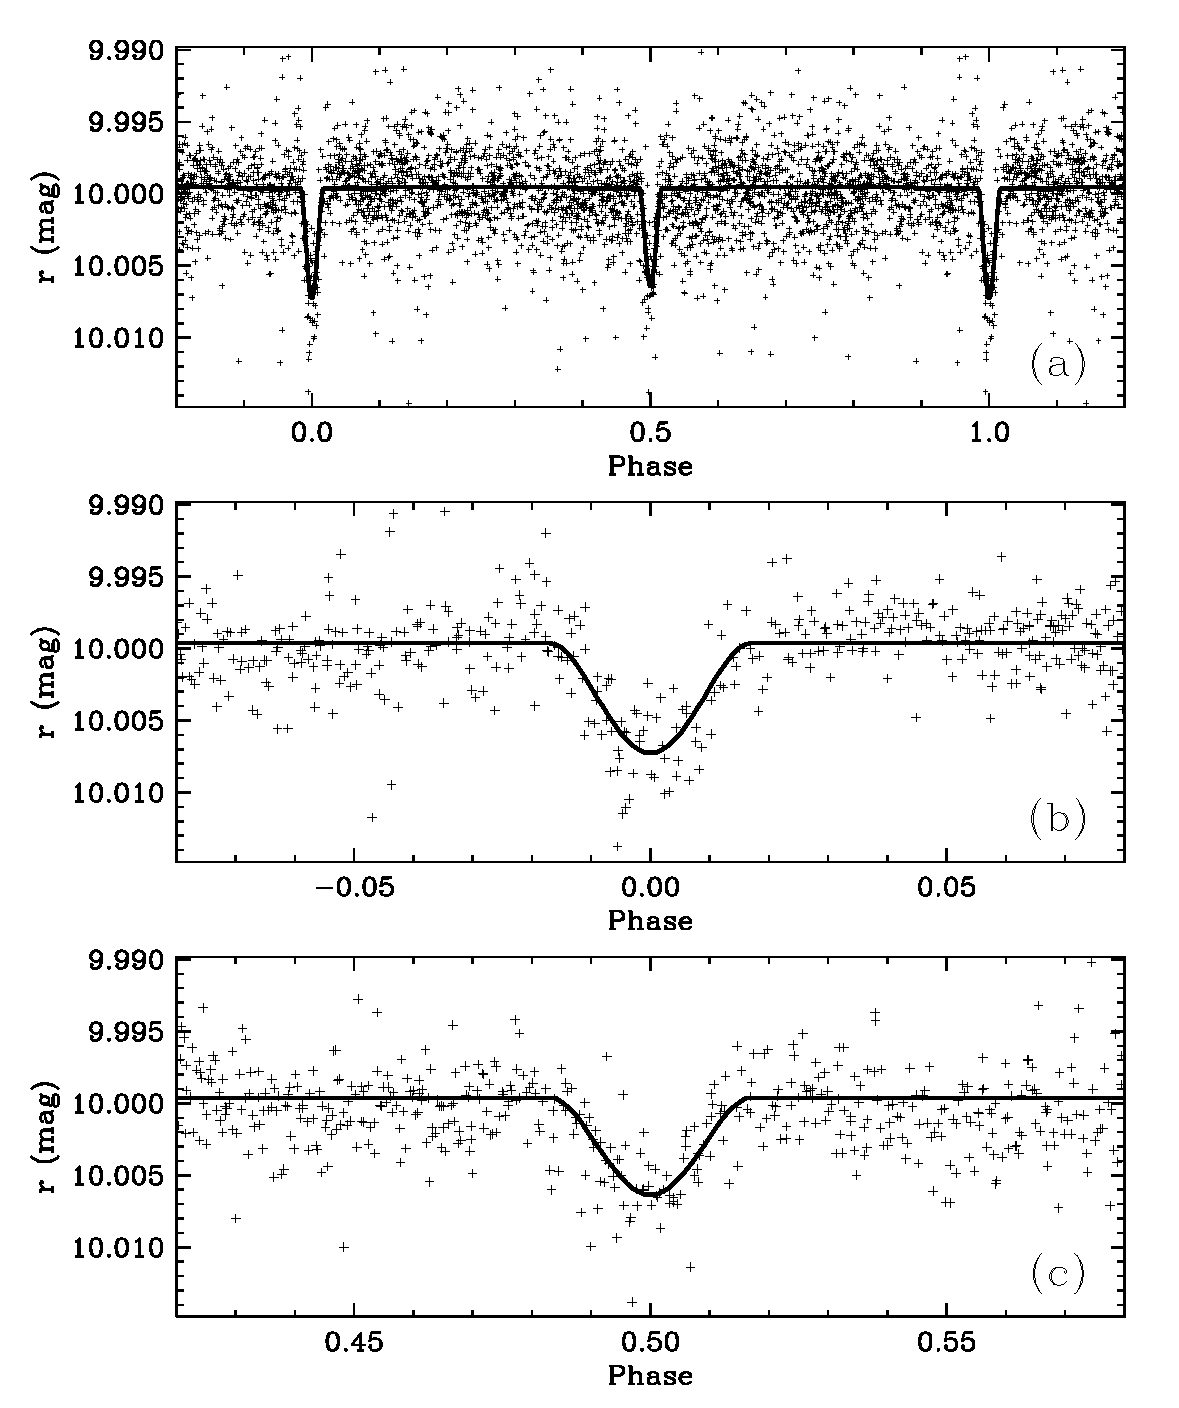
\includegraphics[width=0.95\textwidth]{3_f6}
\caption[$r$-band photometry modeled as an F/K+K blend]{TrES $r$-band photometry of \mbox{GSC 03885-00829}, folded
  using a period twice that of our candidate planet (i.e., $2 \times
  1.441$ days). (a) Best-fit blend model consisting of the bright F
  star and a pair of eclipsing K dwarfs (see text). The theoretical
  curve indicates a small difference in depth between the primary and
  secondary eclipse, (b) Enlargement around the primary eclipse, (c)
  Enlargement around the secondary eclipse. The observed duration of
  the eclipses is well reproduced by the model.}\label{cha:gsc:fig:MMmodel}
\end{center}
\end{figure}

The periods for our transit candidates are calculated assuming each
observed transit is of equal depth. However, when a candidate is in
fact a blended eclipsing binary, the possibility exists that the
primary and secondary eclipses are similar enough in depth to be
confused by our period-finding technique. The BLS algorithm may derive
a best-fit period for such a system that is half of the true value.
Therefore, we explored blend scenarios in which the period is $2
\times 1.441$ days. Figure~\ref{cha:gsc:fig:MMmodel} shows the result of our
best fit to the TrES $r$-band data, in which the eclipsing binary is
composed of two late K stars with masses of 0.67 and
0.64\,\msun, with an orbital inclination of $84\degr$ to the
line of sight.  The model indicates a slight difference in eclipse
depths (see figure~\ref{cha:gsc:fig:MMmodel}a) of about 1\,mmag, although this
difference is only marginally visible in observations themselves.
Enlargements of the two eclipse regions are displayed in the lower
panels of figure~\ref{cha:gsc:fig:MMmodel}.  According to this fit, the time
of the center of transit previously derived (see table~\ref{cha:gsc:tab:gsc})
is, in fact, a time of secondary eclipse; all of the photometric
follow-up observations shown in figure~\ref{cha:gsc:fig:multicolor} were taken
during a secondary eclipse.  The brighter of the K stars (i.e., the
primary of the eclipsing binary) has only $\sim$3\% of the light of
the main F star in the optical, and is below our threshold for
spectroscopic detection.  Figure~\ref{cha:gsc:fig:isochrones} shows the
location of the three stars (the {\textit filled circles}) in the H-R diagram.

According to the blend model described above, the eclipse in the $g$
band (a secondary eclipse) is predicted to be shallower than in the
$r$ band (0.35\% versus 0.7\%), as we indeed observe, although the
measured depth (0.4\%) is slightly deeper than that predicted. We attribute
this to shortcomings in the isochrones used for the blend modeling,
which are not specifically designed for low-mass stars. In particular,
missing opacity sources and other physical ingredients may affect the
theoretical luminosities in the optical ($V$ or $g$) bands
\citep{Baraffe_Chabrier_Allard:aa:1998a,
  Delfosse_Forveille_Segransan:aa:2000a,
  Chabrier_Baraffe_Allard:asp:2005a}, whereas the red and near-infrared magnitudes are presumably more reliable. A sign of this is
seen perhaps in the predicted $V-K$ color for the main F star: the
isochrones give $V-K = 1.26$ \citep[in the Johnson system as defined
by][]{Bessell_Brett:pasp:1988a}, bluer than the typical color of a
dwarf of this temperature, $V-K = 1.40$
\citep[e.g.,][]{Bessell_Brett:pasp:1988a}.  Other stellar evolution
models specifically designed for low-mass stars such as those by
\citet{Baraffe_Chabrier_Allard:aa:1998a} appear to give more realistic
colors. Our F star is predicted to have $V-K = 1.41$ according to
those calculations \citep[after transformation of the isochrone $K$
magnitudes from the CIT to the Johnson system,
following][]{Leggett:apjs:1992}, very close to the empirical
value. Unfortunately the \citet{Baraffe_Chabrier_Allard:aa:1998a}
models are not publicly available for the Sloan bands, so we are
unable to use them in our blend modeling.

\begin{figure}
\begin{center}
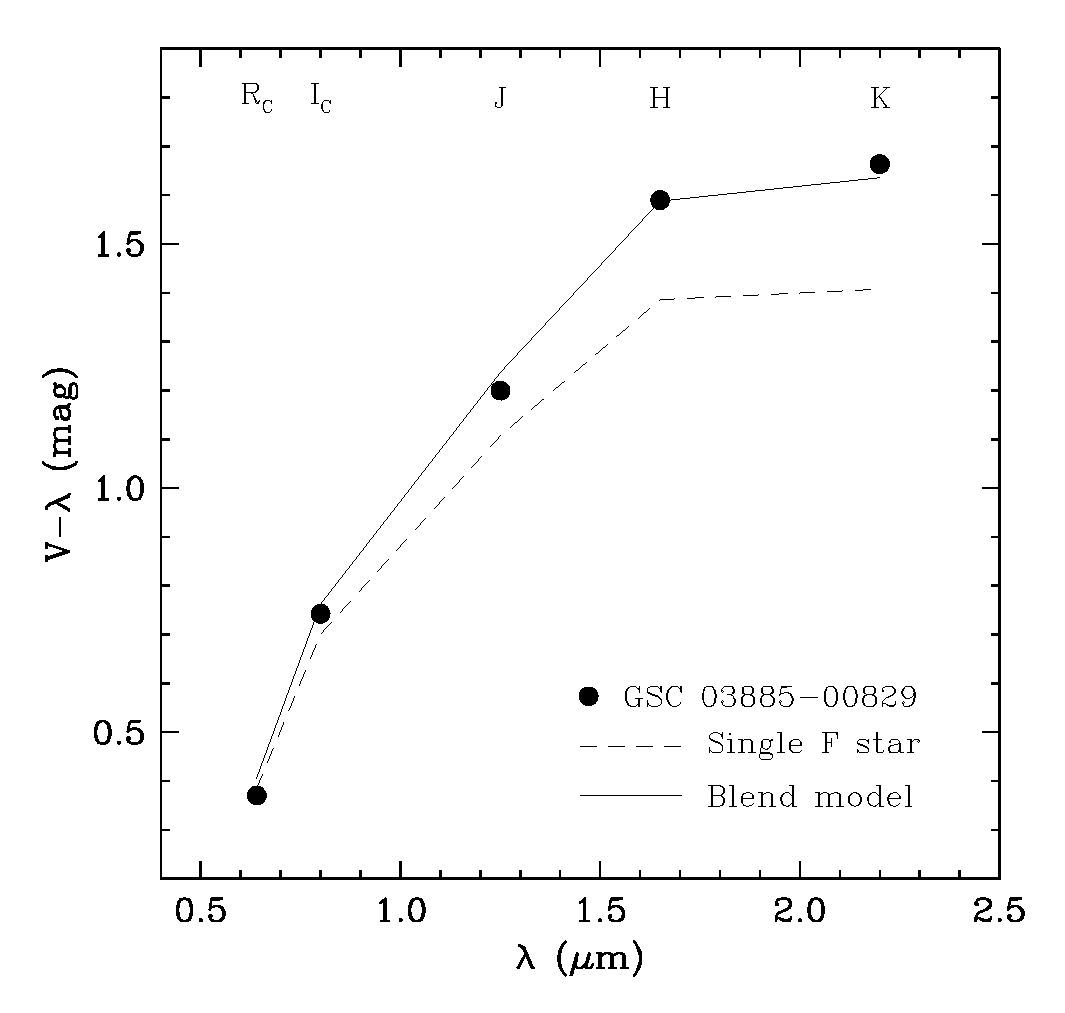
\includegraphics[width=0.95\textwidth]{3_f7}
\caption[Near-infrared colors for \mbox{GSC 03885-00829} and an F star]{Near-infrared colors measured for \mbox{GSC 03885-00829}
  ({\textit dots}) compared with the theoretical colors of a single F star
  ({\textit dashed line}) and the colors from our blend model ({\textit solid line};
  combined light of three stars). The latter is seen to reproduce the
  observed colors well.}\label{cha:gsc:fig:colors}
\end{center}
\end{figure}

As indicated earlier, infrared magnitudes for \gscOTE\ are
available from the 2MASS Catalog.  In particular, the measured $V-K$
color of our candidate in the Johnson system (table~\ref{cha:gsc:tab:gsc}) is
$1.66 \pm 0.02$
\citep[using transformations from the 2MASS system
by][]{Carpenter:aj:2001a}. The difference with the color of a single F star
indicates a significant infrared excess of about a quarter of a
magnitude%
\footnote{Hence, even if we underestimated the error in our $V$-band
  photometry (see section~\ref{cha:gsc:sec:photo}) by an order of magnitude, the
  resulting propagation of error would not significantly affect the
  size of this discrepancy.}%
. This in itself can be taken as evidence of contamination
from the light of a later-type object, providing further evidence that
we are dealing with a blend. The computed color of the combined light
of the three stars in our model using the
 \citet{Baraffe_Chabrier_Allard:aa:1998a} isochrones
is $V-K = 1.64$, which agrees quite well with the observations and
supports our interpretation. Other predicted red and infrared colors
also match the measured values reasonably well (see figure~\ref{cha:gsc:fig:colors}).

Although it is quite possible that additional fine-tuning may improve
the small discrepancies noted above in the $g$ band and provide a
near-perfect fit to all observations (to the extent allowed by the
accuracy of the stellar evolution models and observational
uncertainties), our goal here has been to show how subtle the
signatures of a blend can be, and that with careful modeling it is
possible to demonstrate that they are, in fact, due to a blend scenario
and therefore reject the candidate.

\section{Confirmation of Blend Model}\label{cha:gsc:sec:nirspec}

In order to further test our blend hypothesis, we observed
\gscOTE\ on UT 2005 August~15 with the NIRSPEC
infrared spectrograph at the Keck Observatory.  We observed
the target in the $K$-band spectral region centered near 2.293\,$\mu$m,
to search for the presence of features from the \mbox{$^{12}$CO 2--0} bandhead.
Such features are very weak for mid-G-type stars, and absent for
stars with spectral types earlier than G0.  Hence, the detection
of such features would indicate the presence of a cool stellar
photosphere, as predicted by our blend scenario.

We used a 3-pixel-wide slit, which yields a spectral resolution of
approximately 25,000.  We gathered two 4-minute exposures,
between which we nodded along the slit by roughly $5\arcsec$.
We differenced the two exposures to subtract the sky emission
and any pixel-dependent detector bias.  We extracted the
order spanning the location of the \mbox{$^{12}$CO 2--0} bandhead
by summing over a 15-pixel-wide band centered on the
peak of the instrumental profile.  A small number of
values in the extracted one-dimensional spectrum were corrupted
due to bad pixels in the infrared detector.  We replaced
these values (30 of 1024 pixels) by interpolation.
This region contains a large number of telluric methane features.  We
produced a model of these features by modifying the electronic version of the Kitt Peak National Observatory Fourier Transform Spectrometer (KPNO FTS) telluric spectrum \citep{Livingston_Wallace:NSO:1991a} for air mass,
wavelength-solution, and instrumental PSF.
Dividing our extracted spectrum by this model yields the
stellar spectrum corrected for telluric absorption.

\begin{figure}
\begin{center}
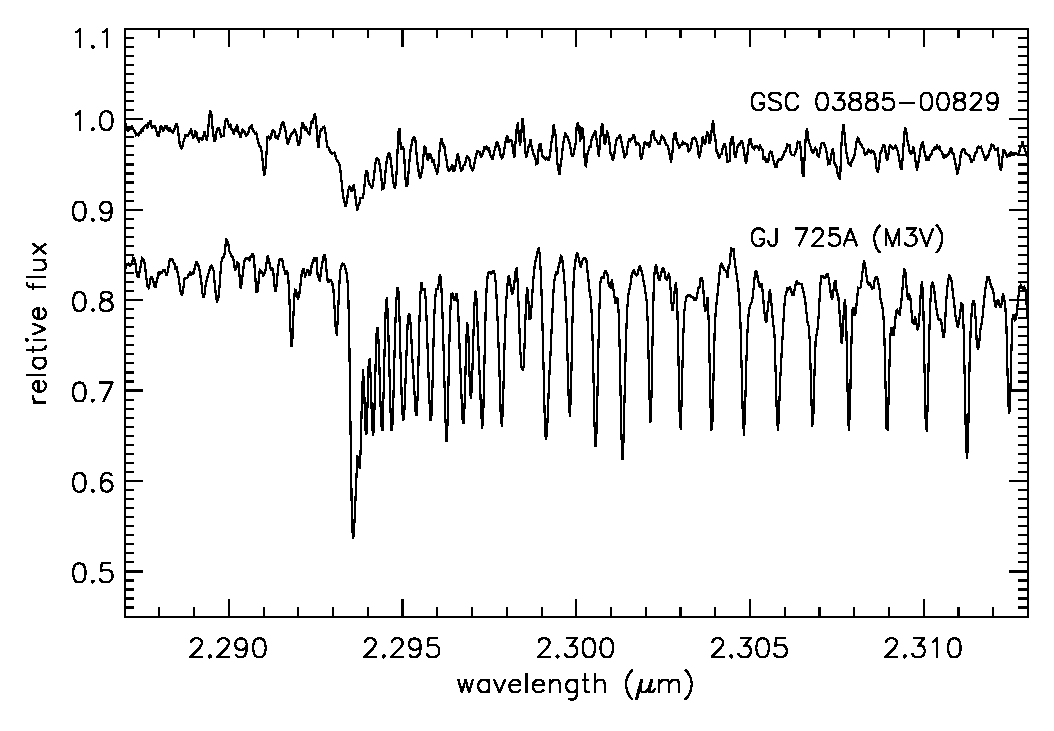
\includegraphics[width=0.95\textwidth]{3_f8}
\caption[Spectrum showing evidence of light from late-type star]{$K$-band spectra of \mbox{GSC 03885-00829} and a nearby
  M3V star (\mbox{GJ\,725A}), obtained with the NIRSPEC spectrograph
  at the Keck Observatory. The M dwarf spectrum, with strong CO
  features, is shown for comparison with our target spectrum, which
  displays the \mbox{$^{12}$CO 2--0} band head at approximately $2.293\,\mu$m. The spectrum must therefore include the light of a star with a spectral
  type later than the F-dwarf target star, such as the K dwarfs of our
  blend model. The presence of the CO feature thus rules out the
  possibility of a planetary companion.}\label{cha:gsc:fig:nirspec}
\end{center}
\end{figure}

In figure~\ref{cha:gsc:fig:nirspec} we plot the resulting spectrum, as well as a
spectrum of the nearby M3V star \mbox{GJ\,725A} (which
shows very prominent CO features) for comparison. The relative intensity
between the individual CO features at 2.3\,$\mu$m does not
differ for these two types of stars, although the overall amplitude of the
features is reduced for hotter temperatures. We did not attempt to match the
spectral type of the NIRSPEC data quantitatively, since our primary goal
is to exclude the planetary hypothesis. The spectrum of
\gscOTE\ clearly shows the \mbox{$^{12}$CO 2--0} bandhead near 2.293\,$\mu$m;
the relative depth of the band head
is approximately 6\%. The detection of this feature confirms
the presence of a cool stellar photosphere. Also, for the late K dwarfs of
our model, the \mbox{$^{12}$CO 2--0} band head has a depth of approximately 30\%,
and the K dwarfs in our blend model contribute 25\% of the $K$-band
flux from the system. Hence the expected depth of this band head in
our spectrum is $\sim$7.5\%, in rough agreement with the observed
relative depth. Thus, we interpret this feature as originating in the
photospheres of the K-stars of the binary.

The Heliocentric Julian day at mid-exposure was HJD 2453597.83591,
which corresponds to an orbital phase of 0.09, at which point the
expected velocity separation between the two K stars is
$89.5\,\mathrm{km\,s^{-1}}$.  The K stars are likely tidally locked,
and hence their spectral features will have a $v \sin{i} =
12\,\mathrm{km\,s^{-1}}$. Since this is smaller than the predicted
velocity separation at the time of the exposure, we might expect to
resolve the individual components of the observed \mbox{$^{12}$CO 2--0} feature
from the two K stars of the binary. And indeed the band head in our
spectrum shows two clear peaks of similar depth, with a velocity
separation similar to the predicted separation of the K dwarfs. A more
careful analysis of this spectrum (e.g., using the two-dimensional cross-correlation algorithm TODCOR;
\citealt{Zucker_Mazeh:apj:1994a}) should recover the components more
precisely. However, for the purposes of this paper, it is enough to
identify the presence of the light from an eclipsing K binary system
in our spectrum, which rules out the transiting planet hypothesis.

\section{The Necessity of Blend Identification}\label{cha:gsc:sec:dis}

The difficult task of eliminating any contamination resulting in a
false transit signal is the primary challenge currently facing wide-field transit surveys. Developing this experience will not only enable
us to make firm detections of transiting Jupiters but will be
extremely valuable as we search for Earth-sized planets outside our
solar system with NASA's {\textit Kepler} mission. As with the
ground-based wide-field surveys, the challenge with {\textit Kepler} will not
only be obtaining the photometric precision necessary to observe these
minute signals, but rejecting all other possible causes of these
eclipses as well.

We have presented here one of our disappointments: a candidate that
passed all of our initial photometric and spectroscopic tests, but was
later shown to be a result of contaminated light from an eclipsing
binary. As such, it highlights the difficulty in rejecting all false
positives from a transit survey. As the components of this eclipsing
binary are both faint K dwarfs, the resultant radial velocity
variations in the light blended with that from the nearby F star are
not detectable. Also, the resultant color dependence of the blended
light curve is small, albeit observable, and the system displays a
color redder than that of an isolated F star.

The TrES survey readily produces on the order of 10 candidate
transiting planets from each selected field of view with
15,000--25,000 stars, the majority of these candidates proving to be
astrophysical false positives.  Some of these will mimic the expected properties of
a planetary system quite closely. On the basis of our experience of frequent
blends, where the telltale indicators of the stellar components are
often masked, spectroscopic and even multicolor photometric
follow-up is insufficient to confirm the planetary nature of a
candidate. An attempt must be made to interpret the observations as
those of a blended eclipsing binary and this interpretation rejected
only if the observations are not in agreement.  Having meticulously
examined the evidence, we can commit to obtain the radial velocity
orbit of this firm candidate through high-resolution spectroscopy with
a high signal-to-noise ratio. It should be emphasized that
determining the mass of the candidate from such observations is a
necessary step in identifying a transiting planet.  The methods for
rejecting astrophysical false positives presented here and by other
authors cannot be used to confirm the planetary nature of a candidate;
rather they increase the yield of planets from the resource-intensive
high-dispersion spectroscopy required for such a confirmation.


% chktex-file 44 chktex-file 15
\chapter[TrES-2: The First Transiting Planet in the Kepler Field]%
{%
TrES-2: The First Transiting Planet in the Kepler Field%
\protect\CFNC%
}\label{cha:tres2}

\section*{Abstract}\label{cha:tres2:sec:abs}
\addcontentsline{toc}{section}{Abstract}

We announce the discovery of the second transiting hot Jupiter
discovered by the Trans-atlantic Exoplanet Survey. The planet, which
we dub \tresTwo, orbits the nearby star \gscOTF\ every 2.47063 days.  From
high-resolution spectra, we determine that the star has $T_{\mathrm
  eff}=5960\pm100\,\mathrm{K}$ and $\log{g}=4.4\pm0.2$, implying a
spectral type of G0V and a mass of $1.08^{+0.11}_{-0.05}\,M_{\sun}$.
High-precision radial-velocity measurements confirm a sinusoidal
variation with the period and phase predicted by the photometry, and
rule out the presence of line-bisector variations that
would indicate that the spectroscopic orbit is spurious.  We estimate
a planetary mass of $1.28^{+0.09}_{-0.04}\,M_{\mathrm Jup}$.  We model
$B$, $r$, $R$, and $I$ photometric timeseries of the 1.4\%-deep
transits and find a planetary radius of $1.24^{+0.09}_{-0.06}\,R_{\mathrm
  Jup}$.  This planet lies within the field of view of the NASA
\textit{Kepler} mission, ensuring that hundreds of upcoming transits
will be monitored with exquisite precision and permitting a host of
unprecedented investigations.

\section{The Search for Transiting Exoplanets}\label{cha:tres2:sec:intro}

Observations of the 10 transiting hot Jupiters known at the time of writing have provided
precise planetary radii and masses, and tested formation and structure
models for extrasolar planets
\citep[see][]{Laughlin_Wolf_Vanmunster:apj:2005a,
  Charbonneau_Brown_Burrows:PPV:2007a}. More detailed studies of the
nearby planets have probed their atmospheres and led to the direct
detection of their thermal emission
\citep[e.g.,][]{Charbonneau_Brown_Noyes:apj:2002a,
  Charbonneau_Allen_Megeath:apj:2005a,
  Deming_Brown_Charbonneau:apj:2005a,
  Deming_Seager_Richardson:nat:2005a}.

Three of these planets were known from radial-velocity surveys of the
solar neighborhood, and were subsequently observed to transit.  The
remaining seven were discovered from photometric observations. The
radial-velocity confirmation of transiting planet candidates involves
extensive use of large-aperture telescopes. With the goal of
maximizing the yield of transiting planets around bright stars and
minimizing the time required of large observatories, several teams are
undertaking wide-field photometric surveys using small telescopes
\citep[for a review, see][]{Charbonneau_Brown_Burrows:PPV:2007a}. Our
collaboration is conducting the Trans-atlantic Exoplanet Survey%
\footnote{See \url{http://www.astro.caltech.edu/\~ftod/tres/}\ .}%
\ (TrES): \tresOne\ was the first nearby transiting planet to be
discovered photometrically \citep{Alonso_Brown_Torres:apjl:2004a}.

Such photometric surveys yield numerous transit candidates, of which
the majority are astrophysical false positives that are discarded by
follow-up photometric and spectroscopic observations
(\citealp[e.g.,][]{ODonovan_Charbonneau_Alonso:apj:2007a}, see chapter~\ref{cha:and0}).
However, eliminating a blend, wherein a bright star forms a chance
superposition or a hierarchical triple with a faint eclipsing binary,
can require a careful analysis
(\citealp[][]{Torres_Konacki_Sasselov:apj:2004b,
  Mandushev_Torres_Latham:apj:2005a}; \citealp{ODonovan_Charbonneau_Torres:apj:2006a}, see chapter~\ref{cha:gsc}).

We present here the discovery of the planet \tresTwo\ and describe the process by which we confirmed its planetary nature and deduced its bulk properties.

\section{Observations and Analysis of \tresTwo}\label{cha:tres2:sec:observations}

Transits of the parent star \tresTwo\ were first observed by Sleuth
(Palomar Observatory, California; \citealt{ODonovan_Charbonneau_Kotredes:AIP:2004a}) and the Planet Search Survey Telescope (PSST;  Lowell Observatory, Arizona; \citealt{Dunham_Mandushev_Taylor:pasp:2004a}), part of the TrES network of ten-centimeter telescopes.
The third telescope, the Stellar Astrophysics and Research on Exoplanets (STARE; \citealt{Alonso_Deeg_Brown:an:2004a}) in Tenerife, Spain, did not observe
because it was undergoing an upgrade at the time. The two telescopes
monitored a $5.7\degr \times 5.7\degr$ field of view (FOV) centered on
the star \mbox{16\,Lyr} from UT 2005 June~16 to September~3.
The analysis of TrES images has been described in detail in
\citet{Dunham_Mandushev_Taylor:pasp:2004a},
\citeauthor{ODonovan_Charbonneau_Torres:apj:2006a}~(\citeyear{ODonovan_Charbonneau_Torres:apj:2006a}, chapter~\ref{cha:gsc}), and
\citeauthor{ODonovan_Charbonneau_Alonso:apj:2007a}~(\citeyear{ODonovan_Charbonneau_Alonso:apj:2007a}, chapter~\ref{cha:and0}).
In summary, we analyzed the Sleuth and PSST images separately.
After calibration, we obtained a list of the field stars in each image and determined
their equatorial coordinates. We applied our image spatial
interpolation and subtraction routines based in part on
\citet{Alard:aas:2000a} to obtain the differential magnitude of each
star in each image. We decorrelated and binned the stellar light curves,
before applying the transit-search
algorithm of \citeauthor*{Kovacs_Zucker_Mazeh:aa:2002a}~(\citeyear{Kovacs_Zucker_Mazeh:aa:2002a}, see appendix~\ref{cha:bls}) to identify stars
showing statistically significant, periodic transit-like events.

\begin{deluxetable}{lc}
\tablewidth{0pt}
\tablecaption{System parameters for TrES-2 planet\label{cha:tres2:tab:tres2b}}
\tablehead{ \colhead{Parameter} & \colhead{Value} }
\startdata
$P$ \phm{000} (days) &  \phm{00000.} $2.47063\pm0.00001$ \\
$T_{c}$ \phm{00.} (HJD)  & $2453957.6358\pm0.0010$ \\
$a$ \phm{000.} (AU) &  \phm{0000} $0.0367^{+0.0012}_{-0.0005}$ \\
$i$ \phm{0000} (deg)  &  \phm{0000} $83.90\pm0.22$  \\
$K$ \phm{000.}($\mathrm{m\,s^{-1}}$) &  \phm{000} $181.3\pm2.6$ \\
$M_{p}$  \phm{00} ($M_{\mathrm Jup}$) &  \phm{000..} $1.28^{+0.09}_{-0.04}$ \\
$R_{p}$ \phm{000}($R_{\mathrm Jup})$ \tablenotemark{a} &  \phm{000..} $1.24^{+0.09}_{-0.06}$ \\
\enddata
\tablenotetext{a}{Here $R_{\mathrm Jup} = 71,\!492$~km, the equatorial radius
  of Jupiter at 1~bar.}
\end{deluxetable}

\begin{figure}
\begin{center}
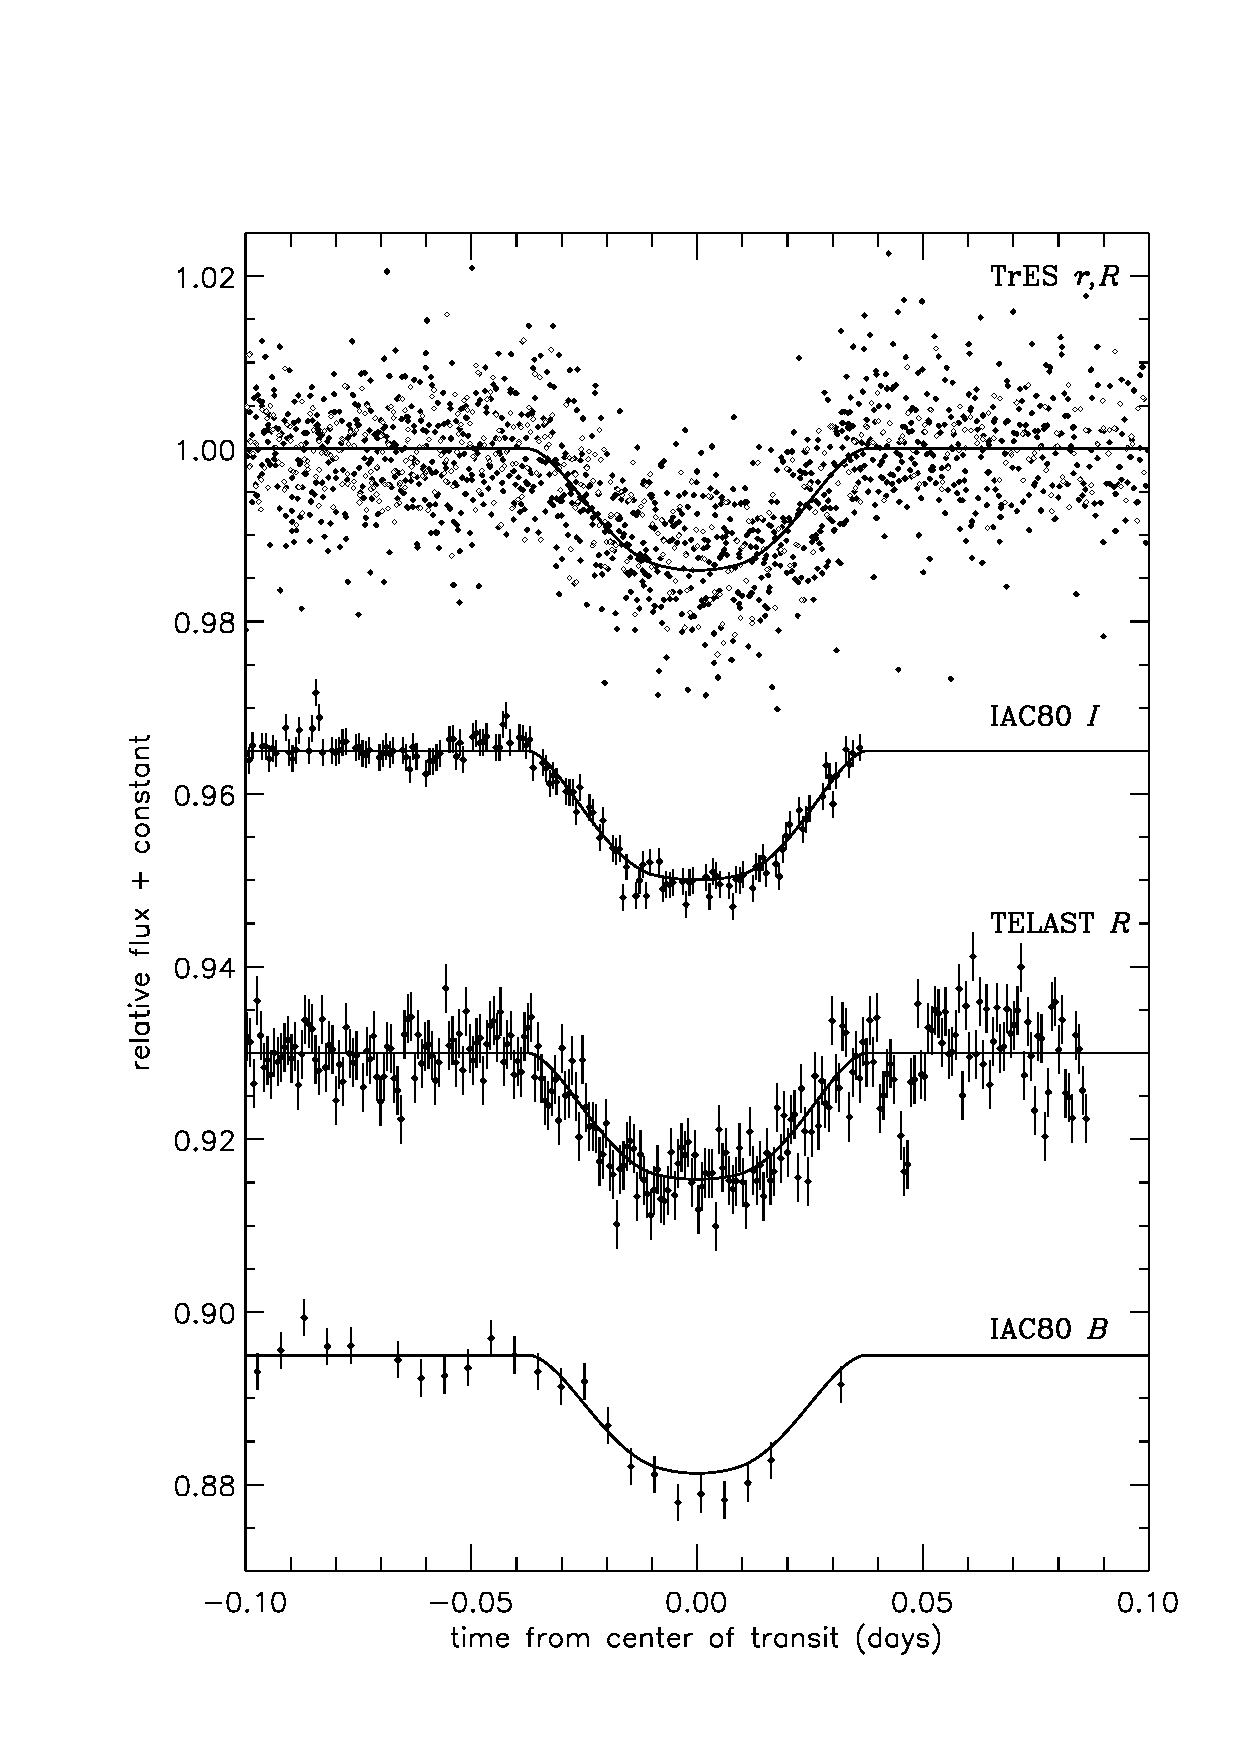
\includegraphics[width=0.95\textwidth]{4_f1}
\caption[Relative flux versus time for the TrES-2 transiting system]{Relative flux of the TrES-2 system as a function of time
  from the center of transit, assuming the ephemeris in
  table~\ref{cha:tres2:tab:tres2b}. The top light curve shows the unbinned
  discovery data, consisting of points from Sleuth $r$ ({\textit filled
    diamonds}) and PSST $R$ ({\textit open diamonds}). Each of the
  follow-up light curves is labeled with the telescope and filter
  employed.  We have overplotted the simultaneous best-fit solution,
  assuming the appropriate quadratic limb-darkening parameters for
  each band pass.}\label{cha:tres2:fig:treslc}
\end{center}
\end{figure}

We quickly selected \tresTwo\ as a prime candidate. The Sleuth $r$ and
PSST $R$ photometric time series obtained near-transit and folded with
a period $P=2.47063$\,days are shown in figure~\ref{cha:tres2:fig:treslc}. Five
full transits and three partial transits were observed by Sleuth. PSST
observed two full transits and one partial event, events that were
also observed by Sleuth. We were therefore confident that the events
were not the result of instrumental error. The depth of 1.4\% was
consistent with the transit of a Jupiter-sized object across a
solar-type star, and the duration of only 1.5\,hr implied a
near-grazing eclipse.

\begin{deluxetable}{lcc}
\tablewidth{0pt}
\tablecaption{System parameters for {TrES-2} parent star\label{cha:tres2:tab:tres2}}
\tablehead{ \colhead{Parameter} & \colhead{Value}  &  \colhead{Reference} }
\startdata
R.A. \phm{00000000.} (J2000.0)  &  \phm{000.}$19^{\mathrm h} 07^{\mathrm m} 14.03^{\mathrm s}$ &  \\
Decl. \phm{00000000} (J2000.0)  &  $+49\degr 18\arcmin 59.3\arcsec$ &  \\
GSC & \mbox{03549-02811} & \\
Spectral Type  &  G0V & 1 \\
$M_{\star}$ \phm{000000000..} ($M_{\sun}$)  &  $1.08^{+0.11}_{-0.05}$  & 1 \\
$R_{\star}$ \phm{0000000000.} ($R_{\sun}$) &  $1.00^{+0.06}_{-0.04}$  & 1 \\
$T_{\mathrm eff}$ \phm{000000000..} (K) &  $5960 \pm 100$ & 1 \\
$\log{g}$ \phm{000000000} (dex) & \phm{.} $4.4 \pm 0.2$ & 1 \\
$v\sin{i}$ \phm{0000000..} (${\mathrm km\, s^{-1}}$) & \phm{.} $2.0 \pm 1.5$ & 1 \\
$V$ \phm{00000000000.} (mag) & $11.411\pm0.005$ & 1 \\
$B-V$ \phm{$0000000.$} (mag) &  \phn$0.619\pm0.009$ & 1 \\
$U-B$  \phm{$0000000.$} (mag) &  \phn$0.112\pm0.012$ & 1\\
$V-R_{\mathrm C}$  \phm{$000000.$} (mag) &  \phn$0.361\pm0.008$ & 1\\
$J$  \phm{000000000000}  (mag) &  $10.232 \pm 0.020$ & 2 \\
$J-H$  \phm{0000000.} (mag) & \phn$0.312 \pm 0.033$ & 2 \\
$J-K_{s}$  \phm{0000000} (mag) & \phn$0.386 \pm 0.030$ & 2 \\
$[\mu_{\alpha},\mu_{\delta}]$ \phm{000000..} ($\mathrm{mas\ yr^{-1}}$) &  $[+4.45,-3.40]$ & 3 \\
\enddata
\tablerefs{%
(1) This work;
(2) 2MASS Catalog;
(3) UCAC2 Bright Star Supplement.%
}
\end{deluxetable}

We searched for the counterpart of \tresTwo\ in publicly available
catalogs and identified the star as \gscOTF.
The 2MASS $J-K_{s}=0.386$\,mag is consistent with a Sun-like star.
The UCAC2
proper motion ($5.60\,\mathrm{mas\,yr^{-1}}$) is also consistent with,
but slightly less than, the expectation for a nearby dwarf. We examined
the DSS images and found no nearby bright companions within the
$30\arcsec$ radius of the Sleuth photometric aperture.
In order to obtain absolute photometry and colors of \tresTwo, we observed it
 in Johnson $UBV$ and Cousins $R$
on the nights of UT 2006 August~29 and~30 with the 105-centimeter Hall telescope at Lowell Observatory.
We calibrated the data using six standard fields \citep{Landolt:aj:1992a},
and the results are given in table~\ref{cha:tres2:tab:tres2}.

We observed
\tresTwo\ using the CfA Digital Speedometers \citep{Latham:ASP:1992a} on
UT 2005 October~18, 20, and~23, November~13, and 2006~June~13.
These spectra are centered on 5187\,\AA\ and cover 45\,\AA\ with
a resolving power of $\lambda / \Delta \lambda \approx 35,\!000$. By
cross-correlating these spectra with synthetic spectra created by
J.~Morse using Kurucz model stellar atmospheres (J.~Morse \&
R.~L.~Kurucz 2004, private communication), we computed the radial
velocity (RV) at each epoch. Within the measurement error
($\sim$0.5\,$\mathrm{km\,s^{-1}}$), the RVs are
constant with a mean velocity of $-0.56\,\mathrm{km\,s^{-1}}$ and a
scatter of $0.55\,\mathrm{km\,s^{-1}}$.
This limits the mass of the companion to be less than 8\,$M_{\mathrm Jup}$.
From a similar cross-correlation analysis, we
estimate (assuming a solar metallicity) the stellar effective
temperature $T_{\mathrm eff}$, surface gravity $\log{g}$, and the
projected rotational velocity $v \sin{i}$ (table~\ref{cha:tres2:tab:tres2}).
These estimates are consistent with the G0V spectral type implied by
the photometry.

We gathered rapid-cadence, high-precision photometric observations in
$I$ and $B$ on UT 2006 August~10 with the CCD camera at the IAC80, an
80-centimeter telescope of the Observatorio del Teide, Tenerife, Spain. The
CCD camera has a FOV of $10\arcmin\times10\arcmin$, corresponding to
$0\farcs33$~pixel$^{-1}$. After calibrating the images, we carried out
aperture photometry with \texttt{vaphot} \citep{Deeg_Doyle:2001a} on the target
and several reference stars of similar brightness in the FOV.  We
constructed an ensemble average of the calibrators, divided the target
by the resulting time series, and renormalized the resulting light
curve by the median of its value prior to the transit event.
Simultaneous $R$ observations were gathered with the TELAST 0.35-meter
telescope, also located at the Teide Observatory, and were analyzed in
a similar fashion.  This telescope is able to follow the target to
larger air mass permitting greater time coverage, but the resulting
light curve showed a residual trend that was likely due to an
imperfect extinction correction. To correct for this, we fit a cubic
polynomial in time to the out-of-transit data, extended the fit across
the complete data set, and divided the data by this function. For each
data set, we estimated the measurement errors from the rms variation of
the data preceding first contact.  The light curves are presented in
figure~\ref{cha:tres2:fig:treslc}.

\begin{deluxetable}{lcc}
\tablewidth{0pt}
\tablecaption{Relative radial-velocity measurements of TrES-2\label{cha:tres2:tab:rvtres2}}
\tablehead{ \colhead{Observation Epoch} & \colhead{Radial Velocity}  &  \colhead{$\sigma_{\mathrm RV}$} \\
\colhead{HJD - $2,\!400,\!000$} & \colhead{m s$^{-1}$}  &  \colhead{m s$^{-1}$}}
\startdata
53949.76054  &  \phm{$-$}135.5   & 6.1 \\
53949.91993  &   \phm{$-$0}96.8   & 6.1 \\
53950.00216  &   \phm{$-$0}58.9   & 7.7 \\
53950.79018  & $-$201.0   & 8.1 \\
53950.93491  & $-$204.8   & 9.0 \\
53950.98051  & $-$201.7   & 9.0 \\
53951.02136  & $-$198.5   & 7.2 \\
53951.75032  &   \phm{$-$0}91.7   & 6.0 \\
53951.84863  &  \phm{$-$}136.7   & 7.0 \\
53951.95209  &  \phm{$-$}140.5   & 7.1 \\
53952.02736  &  \phm{$-$}145.6   & 8.4 \\
\enddata
\end{deluxetable}

In order to confirm the planetary nature of the companion and measure
its mass, we carried out RV observations using Keck/HIRES
\citep{Vogt_Allen_Bigelow:SPIE:1994a} with its I$_2$
absorption cell \citep{Marcy_Butler:pasp:1992a}.  Eleven star + iodine
spectra and one template spectrum were collected on UT 2006 August~2--4,
permitting good sampling of critical orbital phases. We reduced the
data using the MAKEE package written by T. Barlow. Our spectra were
gathered with a resolving power of $\lambda / \Delta \lambda \simeq
71,\!000$ and with exposure times of 15\,minutes, permitting a typical
signal-to-noise ratio of $120\,\mathrm{pixel^{-1}}$.
Our analysis procedure to derive relative RVs incorporates the full modeling of
temporal and spatial variations of the HIRES instrumental profile (%
\citealt*{Valenti_Butler_Marcy:pasp:1995a}; see also
\citealt{Butler_Marcy_Williams:pasp:1996a,
  Korzennik_Brown_Fischer:apj:2000a};
  \citealt*{Cochran_Hatzes_Paulson:aj:2002a}). We model each echelle order
containing I$_2$ lines independently and then calculate the
internal uncertainties for this
star for each observation as the RV scatter about the mean divided
by the square root of the number of spectral orders. The RV
precision achieved by our code is described in
\citet{Alonso_Brown_Torres:apjl:2004a} and
\citet{Sozzetti_Torres_Latham:apj:2006a,
  Sozzetti_Yong_Carney:aj:2006a}. The RV measurements are listed in
table~\ref{cha:tres2:tab:rvtres2}.

\begin{figure}
\begin{center}
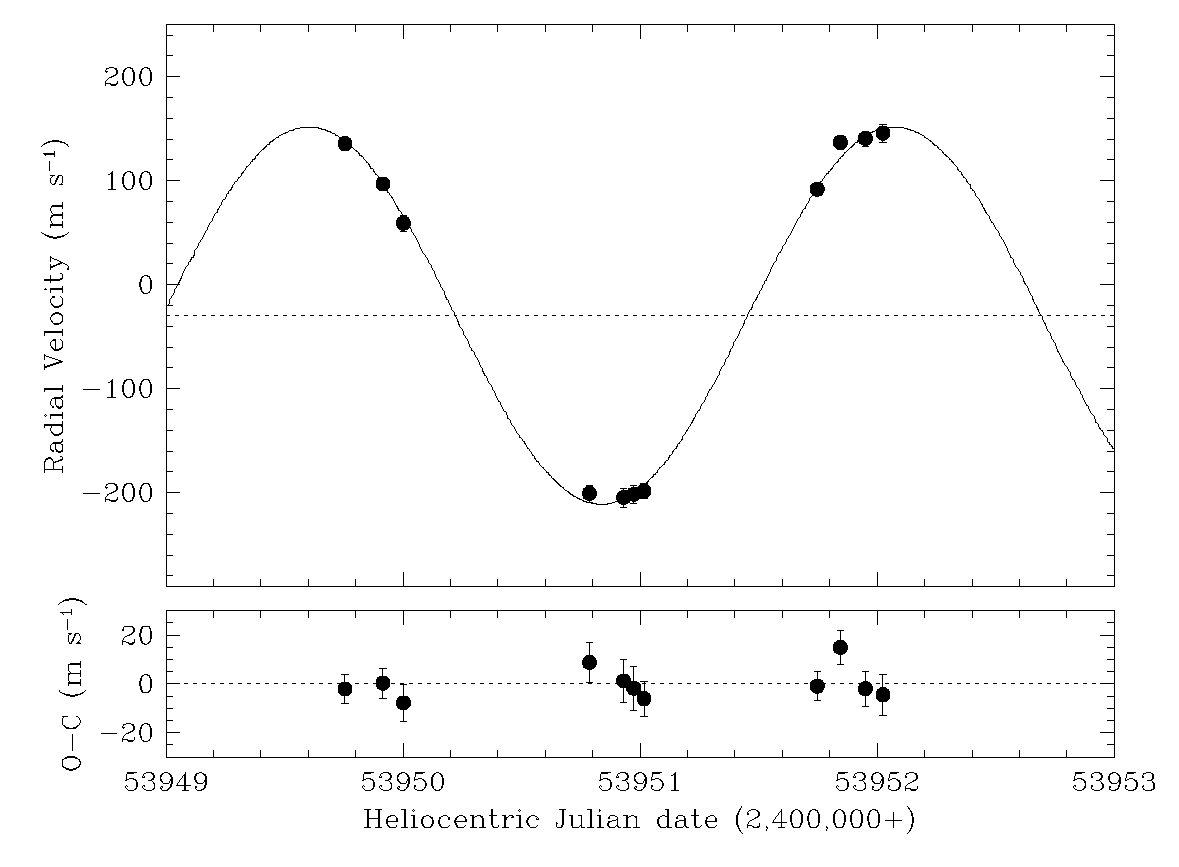
\includegraphics[width=0.95\textwidth]{4_f2}
\caption[Radial-velocity observations of TrES-2]{({\textit Top}) Radial-velocity observations of TrES-2 obtained
  with Keck/HIRES using the I$_{2}$ cell. The best-fit orbit
  (\textit{solid line}) and $\gamma$-velocity (\textit{dashed line})
  are overplotted. ({\textit Bottom}) Residuals from the best-fit
  model to the radial-velocity data.}\label{cha:tres2:fig:rvtres2}
\end{center}
\end{figure}

The best-fit orbital solution, constrained to have zero eccentricity
(as expected from theoretical arguments for a short-period planet),
and with the $P$ and transit epoch $T_{c}$ determined from the
photometric data, yields a velocity semi-amplitude $K =
181.3\pm2.6\,\mathrm{m\,s^{-1}}$ and an instrumental
${\gamma}$-velocity of ${\gamma} = -29.8 \pm 2.2\ {\mathrm m\,
  s^{-1}}$. The fit has a $\chi^2_\nu = 0.89$ ($\nu=9$) and the rms of the
residuals is $6.9\,\mathrm{m\,s^{-1}}$, in excellent agreement with
the internal errors.  Figure~\ref{cha:tres2:fig:rvtres2} shows the RV data
overplotted with the best-fit model, as well as the residuals to the
fit. The parameters of the orbital solution are listed in
table~\ref{cha:tres2:tab:tres2b}. We find a minimum mass for the planet of
$M_{p}\, \sin{i} = 1.206 \pm 0.016\, (\frac{M_p + M_{\star}}{M_{\sun}})^{2/3}\ M_{\mathrm Jup}$,
where $i$ is
the orbital inclination and $M_{\star}$
is the stellar mass.  In section~\ref{cha:tres2:sec:discuss} we estimate these two quantities to obtain
$M_{p}$.  As a further check on the consistency between the
photometric and RV data sets, we fix $P$, set $e=0$, and solve for
$T_c$ (as well as $K$ and ${\gamma}$).  We find $T_{c}=2453957.6283
\pm 0.0084$, which is consistent with, but less precisely determined
than the value predicted from the photometry (table~\ref{cha:tres2:tab:tres2b}).

To investigate the possibility that the RV variations are due not to a
planetary companion but rather to distortions in the spectral line
profiles arising from contamination of the spectrum by an unresolved
eclipsing binary \citep[][]{Santos_Mayor_Naef:aa:2002a,
  Torres_Konacki_Sasselov:apj:2005a}, we examined the line bisectors
carefully for signs of time-varying asymmetries. We cross-correlated
each of our Keck spectra against a synthetic spectrum matching the
measured properties of the star. Line bisectors were then computed
from the cross-correlation function averaged over spectral orders not
affected by the iodine lines, which is representative of the average
spectral line profile.  Bisector spans were calculated as the velocity
difference between points selected near the top and bottom of the
bisectors \citet{Torres_Konacki_Sasselov:apj:2005a}. If the
velocity variations were the result of a stellar blend, we would
expect the bisector spans to vary in phase with the photometric period
with an amplitude similar to that seen in the RVs
\citep{Queloz_Henry_Sivan:aa:2001a, Mandushev_Torres_Latham:apj:2005a}.
 Instead, we did not detect any variation exceeding the measurement uncertainties.

As an additional check we carried out detailed modeling of the TrES
photometry following \citet{Torres_Konacki_Sasselov:apj:2004b} to test
the hypothesis that the light curve is the result of blending the
main G0 star with an unseen eclipsing binary. The properties of the
three stars (parameterized in terms of their mass) were taken from
model isochrones subject to the $T_{\mathrm eff}$ and $\log{g}$
constraints on the main star. An
excellent fit to the TrES $r$-band light curve was obtained for a
triple system composed of a G-dwarf primary blended with an
eclipsing binary with individual components of spectral type M0 and
M4--M5.  In this model, the flux ratio between the G-dwarf primary
and the brightest (M0) component of the blended binary is less than
2\%, which would be undetectable in our spectra.
However, the color difference between the G0 and M0 stars is
such that we would expect the $B$ data to present an eclipse depth
half of that in the TrES bandpass, in contrast to what is observed
(figure~\ref{cha:tres2:fig:treslc}). (Although we note in section~\ref{cha:tres2:sec:discuss}
that a modest color-dependent extinction error may be present in the $B$ data,
it is both the opposite sign and of too small an amplitude to permit the
blend described here.)  More generally, any blend scenario is strongly
disfavored by the observed RV orbit and corresponding lack of bisector
variability.

We conclude from these tests that a blend scenario is strongly
inconsistent with the data, and therefore that the star is indeed
orbited by a Jovian planet.

\section[Estimates of Planet Parameters and Conclusions]{Estimates of Planet Parameters and \\ Conclusions}\label{cha:tres2:sec:discuss}

In order to determine $M_{\star}$ and its uncertainties, we compared
our estimates of $T_{\mathrm eff}$ and $\log{g}$ with evolutionary models
from \citet{Yi_Demarque_Kim:apjs:2001a}, assuming solar
metallicity. For each isochrone, we identified the range of
$M_{\star}$ for which the $T_{\mathrm eff}$ and $\log{g}$ lay within our
1-$\sigma$ errors.  We took the best-fit model as our estimate of
$M_{\star}$ and the span of permitted models (over all ages greater
than 500~Myr) to be our uncertainty.  We then used the resulting
value, $M_{\star} = 1.08^{+0.11}_{-0.05}\, M_{\sun}$, and the
spectroscopic orbit (section~\ref{cha:tres2:sec:observations}) to estimate $M_{p} = 1.28^{+0.09}_{-0.04}\,
M_{\mathrm Jup}$.  We also evaluated the stellar radius $R_{\star}$ in a
similar fashion and found results that were consistent with, but less
tightly constrained than that from the light-curve modeling (below).
The uncertainty contributed by that in the evolutionary models
is less than $0.02\,M_{\sun}$. Based on the absolute visual magnitude
 ($M_{V}$=4.5) predicted
by the best-fit model, we estimate the distance to be approximately
230\,pc. We estimate the reddening in the direction of \tresTwo\ to be
$E(B-V) \sim 0.05$ and the extinction to be $\sim$0.15\,mag from
comparison of its observed colors with the intrinsic
colors predicted by the model.

To estimate $R_{\star}$, $i$, and the planetary radius $R_{p}$, we
simultaneously fit our light curves using the analytical transit
curves of \citet{Mandel_Agol:apjl:2002a} and the color-dependent
quadratic limb-darkening parameters from \citet{Claret:aa:2000a} which
were matched to the spectroscopically estimated properties of the
star.  We identified the best-fit solution by fixing the value of
$M_{\star}$ at its best estimate, $1.08\ M_{\sun}$, and minimizing the
${\chi}^2$ to all the photometry.  We note that the available time
series are well described by the model, with the exception of the
IAC80 $B$, for which the in-transit data fall below the model.  We
speculate that those data, which were gathered at high air mass, may
have been imperfectly corrected for extinction, which is a larger
effect at $B$ than the other band passes.  The best-fit solution
obtains ${\chi}_{\nu}^2=1.15$ ($\nu=2065$), and
its values for $\{R_{\star}, R_{p},i\}$ are listed in tables~\ref{cha:tres2:tab:tres2b}
and~\ref{cha:tres2:tab:tres2}. The
uncertainties in these quantities are dominated by our uncertainty in
$M_{\star}$. To derive 1-$\sigma$ errors for each of $\{R_{\star},
R_{p}, i\}$, we change the value of that parameter and fix it at a new
value, and then allow the other two parameters to float, as well as
allow for a value of $M_{\star}$ within our uncertainty. (The uncertainties in
$P$ and $T_{c}$ are sufficiently small so as not to contribute significantly
to the errors in $R_{\star}$, $R_{p}$, and $i$.) We repeat
this procedure until the best-fit solution produces an increase in the
${\chi}^2$ corresponding to a 1-$\sigma$ change.  Our estimate of the
planetary radius, $R_{p} = 1.24^{+0.09}_{-0.06}\ R_{\mathrm Jup}$, implies
a mean density of $0.83^{+0.12}_{-0.09} \ {\mathrm g\, cm^{-3}}$,
indistinguishable from that of \tresOne\ \citep[using the values
  from][]{Sozzetti_Yong_Torres:apjl:2004a}, despite the fact that
\tresTwo\ is nearly twice as massive. We also note that the impact
parameter, $b = a\, \cos{i} / R_{\star} = 0.84\pm0.02$, is the largest of any
known transiting exoplanet.

We intend to improve our estimates of the planetary and stellar
parameters by undertaking a more detailed analysis of the stellar
spectrum as we did for \tresOne\
\citep{Sozzetti_Yong_Torres:apjl:2004a} and by gathering very
high-precision $z$-band photometry
\citep[e.g.,][]{Holman_Winn_Latham:apj:2006a}.  Such data will
permit us to look for transit timing variations indicative of
additional planets in the \tresTwo\ system
(\citealp{Agol_Steffen_Sari:mnras:2005a}; \citealp{Holman_Murray:Science:2005a}; \citealp{Steffen_Agol:mnras:2005a}). \tresTwo\ lies within the FOV of the NASA
\textit{Kepler} mission. During the four-year mission,
\textit{Kepler} will observe nearly 600 transits of \tresTwo.
The precision with which \textit{Kepler} will observe these transits will
enable an extremely sensitive search for additional planets in the \tresTwo\
system through their dynamical perturbations.  Moreover, the large impact
parameter means that very subtle changes in its value could be detected.
Such variations are predicted \citep{Miralda-Escude:apj:2002a} to occur as a result
of either additional planets, or the stellar quadrupole moment. \textit{Kepler}
may also detect the reflected light from \tresTwo\ \citep{Jenkins_Doyle:apj:2003a}
and hence determine the long-sought geometric albedo and phase function of
a hot Jupiter.
The large impact parameter also makes \tresTwo\ particularly
favorable for determining the angle between the stellar spin-axis and the
orbital axis via the Rossiter-McLaughlin effect
\citep{Gaudi_Winn:apj:2007a}.
\citet{Williams_Charbonneau_Cooper:apj:2006a} discussed
the use of {\textit Spitzer} IRAC observations spanning the time of
secondary eclipse to resolve the surfaces of extrasolar planets.  The
large impact parameter of the \tresTwo\ orbit is ideal for this
application, since it grants access to both longitudinal and
latitudinal flux variations across the dayside hemisphere of the
planet.


\chapter[TrES-3: A Nearby, Massive, Transiting Hot Jupiter in a 31-Hour Orbit]%
{%
TrES-3: A Nearby, Massive, Transiting Hot Jupiter in a 31-Hour Orbit%
\protect\CFND%
}
\label{cha:tres3}

\section*{Abstract}
\label{cha:tres3:sec:abs}
\addcontentsline{toc}{section}{Abstract}

We describe the discovery of a massive transiting hot Jupiter with a very-short orbital period (\mbox{$1.30619$}\,days), which we name \tresThree.
From spectroscopy of the host star \gscOTO, we measure \mbox{$T_{\rm eff} = 5720 \pm 150$\,K}, \mbox{$\log{g}=4.6 \pm 0.3$}, and \mbox{$v\sin{i} < 2\,\kms$}, and derive a stellar mass of $0.90\pm0.15\,M_{\sun}$.
We estimate a planetary mass of \mbox{$1.92 \pm 0.23\,M_{\rm Jup}$}, based on the sinusoidal variation of our high-precision radial-velocity measurements.
This variation has a period and phase consistent with our transit photometry. 
Our spectra show no evidence of line bisector variations that would indicate a blended eclipsing binary star.
From detailed modeling of our $B$ and $z$ photometry of the 2.5\%-deep transits, we determine a stellar radius \mbox{$0.802\pm0.046\,R_{\sun}$} and a planetary radius \mbox{$1.295\pm0.081\,R_{\rm Jup}$}. 
\tresThree\ has one of the shortest orbital periods of the known transiting exoplanets, facilitating studies of orbital decay and mass loss due to evaporation, and making it an excellent target for future studies of infrared emission and reflected starlight.

\section{Transiting Exoplanets with Very-Short Orbital Periods}
\label{cha:tres3:sec:intro}

The OGLE-III deep-field survey \citep[][and references therein]{Udalski_Pietrzynski_Szymanski:acta:2003a} has identified three transiting planetary systems with very short orbital periods: OGLE-TR-56b ($P=29$\,hr; \citealt{Konacki_Torres_Jha:nat:2003a}), OGLE-TR-113b ($P=34$\,hr;  \citealt{Bouchy_Pont_Santos:aa:2004a, Konacki_Torres_Sasselov:apjl:2004a}), and OGLE-TR-132b ($P=41$\,hr;  \citealt{Bouchy_Pont_Santos:aa:2004a}). 
At the time of discovery, such one-day-period planets were conspicuously absent from radial-velocity (RV) surveys. 
These surveys had not discovered a planet with an orbital period of substantially less than 3\,days, despite the sensitivity of such surveys to planets with short orbital periods.
Several authors reconciled this apparent discrepancy by determining the respective observational biases and selection effects (\citealp*{Gaudi_Seager_Mallen-Ornelas:apj:2005a}; \citealp{Pont_Bouchy_Melo:aa:2005a, Gould_Dorsher_Gaudi:acta:2006a, Fressin_Guillot_Morello:preprint:2007a}). 
Since then, hot Jupiters with periods just over two\,days have been detected by both RV surveys (\hdOENb; \citealt{Bouchy_Udry_Mayor:aa:2005a}) and wide-field transit surveys (\wasptwob; Collier Cameron et al., \citeyear{Collier-Cameron_Bouchy_Hebrard:MNRAS:2007a}), indicating a consistent picture for the underlying distribution of orbital periods of hot Jupiters. 

With the discovery of these nearby planets, we continue to observe Sozzetti et al.~(\citeyear{Sozzetti_Torres_Charbonneau:apj:2007a}) the decreasing linear relation between $P$ and the planetary mass ($M_{p}$) for transiting planets  first noticed by \citet*{Mazeh_Zucker_Pont:mnras:2005a} and Gaudi, Seager, \& Mallen-Ornelas~\citeyear{Gaudi_Seager_Mallen-Ornelas:apj:2005a}.
It appears from this small number of planets that shorter period exoplanets are on average more massive.
This may suggest different evolution of these planetary systems than the canonical migration (\citealp[see, e.g.,][]{Trilling_Benz_Guillot:apj:1998a}) of hot Jupiters from beyond the ice line.

We present here the discovery of \tresThree, a massive planet that has the one of the shortest period of the transiting planets, and that was independently identified by two transit surveys. 

\section{Observations and Analysis of \tresThree}
\label{cha:tres3:sec:observations}

Transits of the parent star \gscOTO\ were detected by two ten-centimeter telescopes, part of the Trans-atlantic Exoplanet Survey (TrES) network.
Sleuth (Palomar Observatory, California; \citealt{ODonovan_Charbonneau_Kotredes:AIP:2004a}) observed seven full transits and three partial transits, of which three full and two partial transits were observed by the Planet Search Survey Telescope (Lowell Observatory, Arizona; \citealt{Dunham_Mandushev_Taylor:pasp:2004a}).
We obtained these observations between UT 2006 May~6 and 2006~August~2, during which time we monitored a \mbox{$5\fdg7\times5\fdg7$} field of view (FOV) centered on \thetaher.
We then processed the data from each telescope separately, as we have described previously (\citealp{Dunham_Mandushev_Taylor:pasp:2004a}; \citealp{ODonovan_Charbonneau_Torres:apj:2006a}, see chapter~\ref{cha:gsc}; \citealp{ODonovan_Charbonneau_Alonso:apj:2007a}, see chapter~\ref{cha:and0}).
We then search our binned light curves using the box-fitting transit search algorithm of Kovacs, Zucker, \& Mazeh~(\citeyear{Kovacs_Zucker_Mazeh:aa:2002a}, see appendix~\ref{cha:bls}) for periodic events consistent with the passage of a Jupiter-sized planet across a solarlike star.
We flagged \tresThree\ as a candidate, noting that the transit duration of 1.3\,hr implied a high impact parameter $b$.

Transits of \tresThree\ were independently observed by the Hungarian Automated Telescope Network (HATNet; \citealt{Bakos_Noyes_Kovacs:pasp:2004a}).
We observed the HAT field ``G196'' between UT 2005 June~8 and December~5, using the \mbox{HAT-7} telescope at the Fred~L.\ Whipple Observatory (FLWO) and \mbox{HAT-9} at the Submillimeter Array atop Mauna Kea.
We applied standard calibration and aperture photometry procedures to the frames as described earlier in \citet{Bakos_Noyes_Kovacs:apj:2007a}.
We also applied the trend filtering algorithm \citep{Kovacs_Bakos_Noyes:mnras:2005a} and identified \tresThree\ as a transit candidate using the algorithm of \citet{Kovacs_Zucker_Mazeh:aa:2002a}. 

We observed \tresThree\ using the CfA Digital Speedometers \citep{Latham:ASP:1992a} on 13 occasions from 2006~September~9 to 2007~April~6. 
These spectra are centered at 5187\,\AA\ and cover 45\,\AA\ with a resolving power of \mbox{$\lambda/\Delta\lambda \approx 35,\!000$}.
We derived RVs at each epoch by cross-correlation against synthetic spectra created by J.~Morse using Kurucz model stellar atmospheres (J.~Morse \& R.~L.~Kurucz~2004, private communication).
There is no significant variation in these measurements, which have a mean of \mbox{+9.58\,\kms} and a scatter of \mbox{0.73\,\kms}.
This limits the mass of the companion to be less than $\sim$7\,\mjup.
We estimated the stellar parameters from a cross-correlation analysis similar to that above, assuming a solar metallicity.
The effective temperature ($T_{\rm eff}$), surface gravity ($\log g$), and projected rotational velocity ($v \sin i$) we derive are listed in table~\ref{cha:tres3:tab:tres3}.
On the basis of these values, we estimate the stellar mass to be $M_{\star}=0.90\pm0.15\,M_{\sun}$.
Further spectroscopic analysis of the parent star (similar to that performed for \tresOne\ and \tresTwo; \citealt{Sozzetti_Yong_Torres:apjl:2004a, Sozzetti_Torres_Charbonneau:apj:2007a}) is in progress and will be presented elsewhere.

\begin{deluxetable}{lcc}
\tablewidth{0pt}
\tablecaption{TrES-3 parent star \label{cha:tres3:tab:tres3}}
\tablehead{ \colhead{Parameter} & \colhead{Value}  &  \colhead{Reference} }
\startdata
R.A. \phm{0000000...} (J2000.0)  &  \phm{0}$17^{\rm h} 52^{\rm m} 07.03^{\rm s}$ &  \\
Decl. \phm{0000000..} (J2000.0)  &  $+37\degr 32\arcmin 46.1\arcsec$ &  \\
GSC & \mbox{03089-00929} & \\
$M_{\star}$ \phm{000000000..} ($M_{\sun}$)  &  \phm{..}$0.90\pm0.15$  & 1 \\ 
$R_{\star}$ \tablenotemark{a} \phm{0000000000} ($R_{\sun}$) &  \phm{0}$0.802 \pm 0.046$  & 1 \\ 
$T_{\rm eff}$ \phm{000000000..} (K) & $5720 \pm 150$ & 1 \\ 
$\log{g}$ \phm{00000000..} (dex) & \phm{0}$4.6 \pm 0.3$ & 1 \\ 
$v\sin{i}$ \phm{0000000..} (${\rm km\, s^{-1}}$) & $< 2$ & 1 \\ 
$V$ \phm{00000000000.} (mag) & $12.402\pm0.006$ & 1 \\ 
$B-V$ \phm{0000000.} (mag) &  \phn$0.712\pm0.009$ & 1 \\
$V-R_{\rm C}$  \phm{$000000.$} (mag) &  \phn$0.417\pm0.010$ & 1\\
$V-I_{\rm C}$  \phm{$0000000$} (mag) &  \phn$0.799\pm0.010$ & 1\\
$J$  \phm{000000000000}  (mag) &  $11.015 \pm 0.022$ & 2 \\
$J-H$  \phm{0000000.} (mag) & \phn$0.360 \pm 0.030$ & 2 \\
$J-K_{s}$  \phm{0000000} (mag) & \phn$0.407 \pm 0.028$ & 2 \\
$[\mu_{\alpha},\mu_{\delta}]$ \phm{0000000} ($\mathrm{mas\ yr^{-1}}$) &  $[-22.5, +32.0]$ & 3 \\
\enddata
\tablerefs{%
(1) This work; 
(2) 2MASS Catalog;
(3) UCAC2 Bright Star Supplement.%
}
\tablenotetext{a}{%
The uncertainty in $R_{\star}$ includes both the statistical error and the 5.6\% uncertainty resulting from uncertainty in $M_{\star}$.%
}
\end{deluxetable}

The 2MASS $J-K_{s}$ color (0.407\,mag) and UCAC2 proper motion (39.1 mas yr$^{-1}$) of \gscOTO\ are as expected for a nearby G dwarf. 
We obtained absolute $BVR_{C}I_{C}$ photometry for \tresThree\ on the night of UT 2007 April~14 with the 105-centimeter Hall telescope at Lowell Observatory.
The photometry was calibrated using seven standard fields from \citet{Landolt:aj:1992a}. 
The results are listed in table~\ref{cha:tres3:tab:tres3}.

We observed a full transit in the $z$ band on UT 2007 March~26 using KeplerCam \citep[see, e.g.,][]{Holman_Winn_Latham:apj:2006a} at the \mbox{FLWO 1.2-meter} telescope. 
We obtained 150, 90-s exposures of a $23\farcm1 \times 23\farcm1$ FOV containing \tresThree. 
We observed another transit in Bessell $B$ on UT 2007 April~8 with the Las Cumbres Observatory Global Telescope two-meter Faulkes Telescope North on Haleakala, Maui, Hawaii. 
The CCD camera imaged a $4.6\arcmin$ square field with an effective pixel size of $0\farcs28$ (the images were binned $2\times2$). 
We obtained 126 images with an exposure time of 60\,s and a cadence of 70\,s.
We defocused the telescope slightly (to an image diameter of $\sim$3$\arcsec$) to avoid saturation of the brightest comparison star.
We analyzed these data sets separately.
Using standard IRAF procedures, we corrected the images for bias, dark current, and flat-field response.
We determined fluxes of the target star and numerous comparison stars using synthetic aperture photometry.
To correct the target star fluxes for time-varying atmospheric extinction, we divided them by a weighted average of the fluxes of all the comparison stars.

\begin{deluxetable}{lcc}
\tablewidth{0pt}
\tablecaption{Relative radial-velocity measurements of TrES-3 \label{cha:tres3:tab:rvtres3}}
\tablehead{ \colhead{Observation Epoch} & \colhead{Radial Velocity}  &  \colhead{$\sigma_{\rm RV}$} \\
 \colhead{HJD - $2,\!400,\!000$} & \colhead{m s$^{-1}$}  &  \colhead{m s$^{-1}$}}
\startdata
54186.99525 &   \phm{.}229.0 &  10.8 \\
54187.11354 &    \phm{$.0$}82.1 &    \phm{$0$}8.5 \\
54187.96330 &   \phm{.}167.5 &   \phm{$0$}8.4 \\
54188.04216 &   \phm{.}286.3 &   \phm{$0$}9.7 \\
54188.96503 & -336.5 &   \phm{$0$}8.6 \\
54189.04672 & -234.5 &  10.9 \\
54189.09622 & -183.9 &   \phm{$0$}9.3 \\
\enddata
\end{deluxetable}
 

We collected high-precision RV measurements on UT 2007 March~27--29 using HIRES \citep{Vogt_Allen_Bigelow:SPIE:1994a} and its I$_2$ absorption cell on the Keck~I telescope. 
We obtained a total of seven star+iodine exposures and one template spectrum.
All spectra were gathered with a nominal resolving power \mbox{$\lambda/\Delta\lambda\simeq 55\,000$}, using the HIRES setup with the $0.86\arcsec$ slit.
We used an integration time of 15\,minutes, which yielded a typical signal-to-noise ratio of \mbox{$110\,\mathrm{pixel}^{-1}$}. 
We reduced the raw spectra using the MAKEE software written by T.~Barlow. 
We have described the software used to derive relative radial velocities with an iodine cell in earlier works (\citealp[e.g.,][]{ODonovan_Charbonneau_Mandushev:apjl:2006a}, see chapter~\ref{cha:tres2}; \citealp{Sozzetti_Torres_Latham:apj:2006a}).
We estimate our internal errors from the scatter about the mean for each spectral order divided by the square root of the number of orders containing I$_2$ lines and find them to be around $10\,\ms$.
The radial-velocity measurements are listed in table~\ref{cha:tres3:tab:rvtres3}.

\begin{deluxetable}{lc}
\tablewidth{0pt}
\tablecaption{TrES-3 planet \label{cha:tres3:tab:tres3b}}
\tablehead{ \colhead{Parameter} & \colhead{Value} }
\startdata
$P$ \phm{00..} (days) &  \phm{000000} $1.30619\pm 0.00001$ \\ 
$T_{c}$ \phm{000} (HJD)  & \phm{.}$2454185.9101\pm 0.0003$ \\ 
$a/R_{\star}$ & \phm{000000.}$6.06 \pm 0.10$ \\ 
$a$ \phm{0000} (AU) &  \phm{000000} $0.0226\pm0.0013$ \\ 
$b=a \cos{i} / R_{\star}$ & \phm{000000.}$0.8277 \pm 0.0097$ \\ 
$i$ \phm{0000.} (deg)  &  \phm{00000} $82.15\pm0.21$  \\ 
$K$ \phm{0000}($\mathrm{m\,s^{-1}}$) &  \phm{0000} $378.4\pm9.9$ \\ 
$\gamma$ \phm{0000.}($\mathrm{m\,s^{-1}}$) &  \phm{000.} $-70.6\pm6.2$ \\ 
$M_{p}$  \phm{00.} ($M_{\rm Jup}$) &  \phm{000000} $1.92 \pm 0.23$ \\ 
$R_{p}/R_{\star}$ &  \phm{000000} $0.1660 \pm 0.0024$ \\ 
$R_{p}$ \tablenotemark{a}  \phm{00..}($R_{\rm Jup}$) \tablenotemark{b} &  \phm{000000} $1.295 \pm 0.081$ \\ 
\enddata
\tablenotetext{a}{%
The uncertainty in $R_p$ includes both the statistical error and the 5.6\% uncertainty resulting from uncertainty in $M_{\star}$ (table~\ref{cha:tres3:tab:tres3}).%
}
\tablenotetext{b}{%
Here, $R_{\rm Jup} = 71,\!492$~km, the equatorial radius of Jupiter at 1~bar.%
}
\end{deluxetable}
 
\begin{figure}
\begin{center}
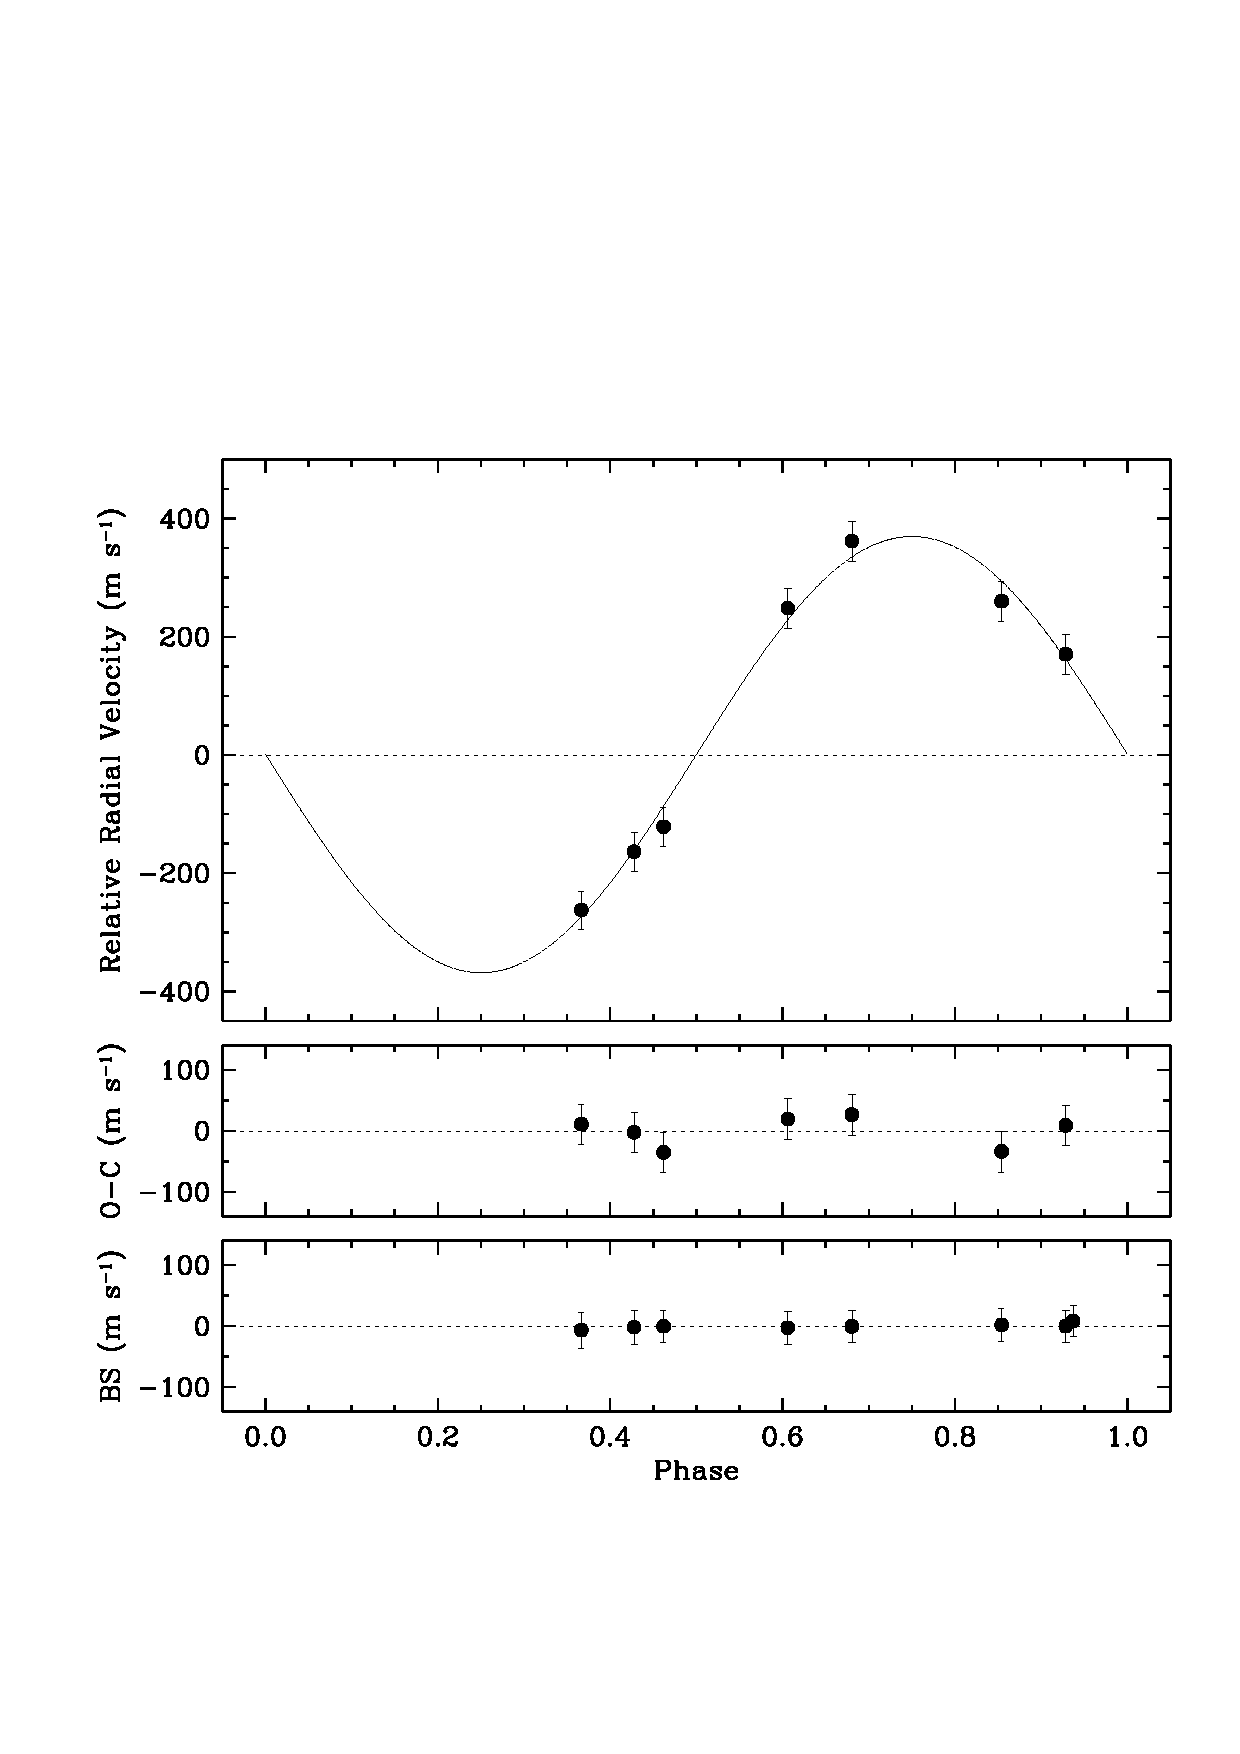
\includegraphics[width=0.95\textwidth]{5_f1}
\caption[%
Radial-velocity observations of TrES-3]{%
({\it Top}) Radial-velocity observations of TrES-3 obtained with Keck/HIRES using the
$\mathrm{I}_2$ cell, shown relative to the center of mass and adopting the ephemeris in table~\ref{cha:tres3:tab:tres3b}. 
The best-fit orbit ({\it solid line}) is overplotted.
({\it Middle}) Residuals from the best-fit model to the radial velocities.
({\it Bottom}) Bisector spans shifted to a median of zero, for each of the iodine exposures as well as for the template (which is shown as the additional data point at phase 0.937).%
}
\label{cha:tres3:fig:rvtres3}
\end{center}
\end{figure}

We constrained the orbital fit to these data to have zero eccentricity ($e$), as expected from theoretical arguments for such a short-period planet, and we also held $P$ and the transit epoch $T_c$ fixed at their values determined from the photometric data. 
The rms residual from this fit (15.4\,\ms) is larger than the typical internal errors (10\,\ms).
Preliminary analysis of the template spectrum suggests that the star shows evidence of activity.
For the inferred spectral type, the presence of radial-velocity ``jitter'' of \mbox{10--20\,\ms} is not unexpected (\citealp*{Saar_Butler_Marcy:apjl:1998a}; \citealp{Santos_Mayor_Naef:aa:2000a, Wright:pasp:2005a}) and would explain the excess scatter we find.
Figure~\ref{cha:tres3:fig:rvtres3} displays the RV data overplotted with the best-fit model, along with the residuals from the fit.
The parameters of the orbital solution are listed in table~\ref{cha:tres3:tab:tres3b}.
We find a minimum planetary mass of \mbox{$M_p \sin i = 2.035 \pm 0.090 [(M_p+M_{\star})/M_{\sun}]^{2/3} M_{\rm Jup}$}, where $i$ represents the orbital inclination. 
As a consistency check we repeated the fit with $P$ fixed and $e = 0$ as before, but
solving for $T_c$.
The result is $T_c = \mathrm{HJD}\,2,\!454,\!185.911 \pm 0.045$, which is consistent with, but less precise than, the value determined from the photometry (table~\ref{cha:tres3:tab:tres3b}).

We investigated the possibility that the velocity variations are due not to a planetary companion but instead to distortions in the line profiles caused by an unresolved eclipsing binary \citep{Santos_Mayor_Naef:aa:2002a, Torres_Konacki_Sasselov:apj:2005a}. 
We cross-correlated each spectrum against a synthetic template matching the properties of the star and averaged the correlation functions over all orders blueward of the region affected by the iodine lines.
From this representation of the average spectral line profile we computed the mean bisectors, and as a measure of the line asymmetry we calculated the ``bisector spans'' as the velocity difference between points selected near the top and bottom of the mean bisectors \citep{Torres_Konacki_Sasselov:apj:2005a}.
If the velocity variations were the result of a stellar blend, we would expect the bisector spans to vary in phase with the photometric period with an amplitude similar to that seen in the RVs \citep{Queloz_Henry_Sivan:aa:2001a, Mandushev_Torres_Latham:apj:2005a}.
Instead, we do not detect any variation exceeding the measurement uncertainties (see figure~\ref{cha:tres3:fig:rvtres3}). 
We conclude that the RV variations are real, and the star is indeed orbited by a Jovian
planet.

\section[Estimates of Planet Parameters and Conclusions]{Estimates of Planet Parameters and \\ Conclusions} 
\label{cha:tres3:sec:discuss}

We analyze our photometric time series using the analytic transit curves of \citet{Mandel_Agol:apjl:2002a} and the Markov Chain Monte Carlo (MCMC) techniques described in \citet{Holman_Winn_Latham:apj:2006a}, \citet{Charbonneau_Winn_Everett:apj:2007a}, and \citet*{Winn_Holman_Roussanova:apj:2007a}.
We assume a circular orbit of constant $P$.
We first estimate $T_c$ by fitting a model light curve (as described below) to only the $z$ data. 
We then determine $P$ by phase-folding the $z$ data with the TrES and HAT discovery data (which affords a baseline of 1.8\,yr) while varying the trial values for $P$. 
We then fix the values for $T_c$ and $P$ (stated in table~\ref{cha:tres3:tab:tres3b}) in the subsequent analysis.

The values of the planet radius $R_p$ and the stellar radius $R_{\star}$ as constrained by the light curves are covariant with $M_{\star}$. 
In our MCMC analysis, we fix $M_{\star} = 0.9\,M_{\sun}$ and then estimate the systematic error in the radii using the scaling relations $R_p \propto R_{\star} \propto M_{\star}^{1/3}$ (see table~\ref{cha:tres3:tab:tres3}, footnote~a). 
We assume a quadratic limb-darkening law with coefficients fixed at the band-dependent values tabulated in \citet{Claret:aa:2000a, Claret:aa:2004a} for the spectroscopically estimated $T_{\rm eff}$ and $\log{g}$ and assuming solar metallicity.

\begin{figure}
\begin{center}
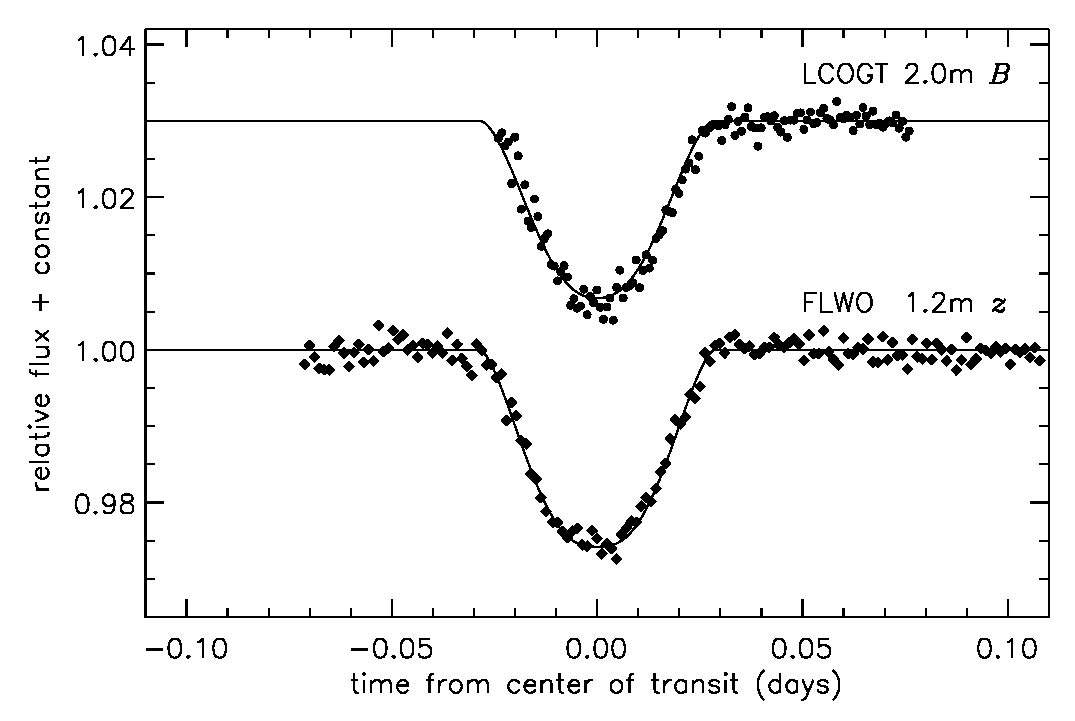
\includegraphics[width=0.95\textwidth]{5_f2}
\caption[%
Relative flux versus time for the TrES-3 transiting system]{%
Relative flux of the TrES-3 system as a function of time from the center of transit, adopting the ephemeris in table~\ref{cha:tres3:tab:tres3b}, and including the residual color-dependent extinction correction (section~\ref{cha:tres3:sec:discuss}). 
Each of these follow-up light curves is labeled with the telescope and filter employed. 
We have overplotted the simultaneous best-fit solution, adopting the appropriate quadratic limb-darkening parameters for each band pass.%
}
\label{cha:tres3:fig:treslc}
\end{center}
\end{figure}

The remaining free parameters in our model are $R_p$, $R_{\star}$, and $i$. 
We require two additional parameters, $k_B$ and $k_z$, the respective residual color-dependent extinction to the $B$ and $z$ light curves, assuming that the observed flux is proportional to $\exp{(-k\, m)}$, where $m$ denotes the air mass. 
We find that the TrES and HAT discovery data are too noisy to meaningfully constrain the parameters, and so we restrict our analysis to the $B$ and $z$ data. 
We first find the values of $R_p$, $R_{\star}$, $i$, $k_B$, and $k_z$ that minimize ${\chi}^2$ using the AMOEBA algorithm \citep[][]{Press_Teukolsky_Vetterling:1992a}.
This model is shown as the solid curves in figure~\ref{cha:tres3:fig:treslc}. 
We then created two MCMC chains with $428,\!000$ points each, one starting from the best-fit values and one starting from a randomly generated perturbation to these values. 
We subsequently rejected the first $100,\!000$ points to minimize the effect of the initial conditions, and found the results of the two chains to be indistinguishable.
We then examined the histograms of the five input parameter values, as well as the histograms for several combinations of parameters relevant to anticipated follow-up studies. 
We assigned the optimal value to be the median and the 1-$\sigma$ error to be the symmetric range about the median that encompassed 68.3\% of the values. 
We state our estimates of the parameters in table~\ref{cha:tres3:tab:tres3b}.
The estimated values for $k_B$ ($0.0029 \pm 0.0006$) and $k_z$ ($-0.0021 \pm 0.0004$) are small and of opposite sign, which is consistent with a modest difference between the average color of the calibration field stars and the target.

Despite the V-shaped transit, our best-fit values indicate that  \tresThree\ is not grazing, i.e., the disk of the planet is entirely contained within the disk of the star at mid-transit, although grazing solutions are permitted by the data. 
Importantly, our ability to obtain well-constrained estimates of $R_{p}$ and $R_{\star}$ despite the large $b$ hinged on having observations of the transit in both $B$ and $z$. 
The large difference in central wavelength and hence stellar limb-darkening between these two bands permitted us to rule out a family of degenerate solutions that is allowed by observations in only a single color. 
We tested this notion by repeating the analysis above for only the $z$ data and found that values of $R_p$ as large as $2.0\,R_{\rm Jup}$ could not be excluded.

\tresThree\ presents a useful testbed for theoretical models of gas giants.
Its radius places it in the growing family of planets with radii that exceed that predicted for models of irradiated gas giants. 
It is one of the most massive transiting planets and has one of the the shortest periods.
We recall that the discovery of \ogletrFSb\ at a distance of only 0.023\,AU from its star stimulated investigations into the timescales for orbital decay and thermal evaporation. 
The comparable orbital separation of \tresThree\ implies that many of these estimates are directly applicable to the new planet, but with the important difference that the much brighter apparent magnitude affords the opportunity for more precise study.
In particular, we note that direct searches for decay of the orbital period may inform our understanding of dissipation in stellar convective zones \citep{Sasselov:apj:2003a}, particularly since both the \tresThree\ planet and its stellar convective zone are more massive than that of \ogletrFSb.
Furthermore, the mass and orbital separation of \tresThree\ are intriguingly close to the critical values estimated by \citet{Baraffe_Selsis_Chabrier:aa:2004a}, below which evaporation would become a dominant process.
The measurement of the angle between the planetary orbit and stellar spin axis of \tresThree\ may detect the substantial misalignment that might be expected for planets that were tidally captured rather than migrating inward \citep{Gaudi_Winn:apj:2007a}.
Assuming isotropic emission, the equilibrium temperature of \tresThree\ is $1643(1-A)^{1/4}$\,K, where $A$ is the Bond albedo. 
We intend to obtain {\it Spitzer} observations of \tresThree, as we have previously done for \tresOne\ and \tresTwo.
Finally, we note that \tresThree\ is extremely favorable for attempts to detect reflected starlight \citep{Charbonneau_Noyes_Korzennik:apjl:1999a, Leigh_Collier-Cameron_Udry:mnras:2003a, Rowe_Matthews_Seager:apj:2006a} and thus determine the geometric albedo, $p_{\lambda}$ of the planet.
The flux of the planet near opposition relative to that of the star is $p_{\lambda} \times (R_p / a)^2 = p_{\lambda} \times 7.5 \times 10^{-4}$, which is more than twice that of any of the other known nearby transiting planets.



\chapter[Detection of Planetary Emission from TrES-2 using \emph{Spitzer}/ IRAC]
{%
Detection of Planetary Emission from TrES-2 using \emph{Spitzer}/IRAC%
\protect\CFNE%
}
\label{cha:spitzer}

\section*{Abstract}
\label{cha:spitzer:sec:abs}
\addcontentsline{toc}{section}{Abstract}

With the discovery of nine new transiting planets within the last year, there have been ample candidates for Target of Opportunity observations using the {\it Spitzer Space Telescope}.
We present here the results of the first of two planned series of observations of \tresTwo\ using the Infrared Array Camera on \spi.
\tresTwo\ is the most massive such candidate to be observed with \spi.
The brightness of this transiting system is seen to decrease by \mbox{$0.168 \pm 0.022$\,\%} at 4.5\,$\mu$m, and \mbox{$0.253 \pm 0.045$\,\%} at 8.0\,$\mu$m, during the secondary eclipse when the planetary emission is blocked by the star.
We show that these flux contrasts are well fit by a blackbody spectrum (similar to the results from recent infrared observations of transiting hot Jupiters) with \mbox{$T_{\rm eff}=1450$\,K}, as well as by a more detailed model spectrum with a planetary $T_{\rm eff}$ of 1550\,K and near-uniform redistribution of the stellar insolation.
The time of the center of the secondary eclipse of \tresTwo\ is found to be consistent with predictions based on recent observations of transits of \tresTwo.
This implies that \tresTwo\ mostly likely has a circular orbit, and thus does not obtain additional thermal energy from tidal dissipation of a nonzero orbital eccentricity.

\section[\textit{Spitzer} Observations of the Known Transiting Exoplanets]{\textbf{\textit{Spitzer}} Observations of the Known Transiting Exoplanets}
\label{cha:spitzer:sec:intro}

There has been a recent dramatic increase in the number of nearby ($d<300$\,pc) extrasolar planets whose structures and atmospheric compositions can be probed using the {\it Spitzer Space Telescope}.
These are the nearby transiting exoplanets (14 at the time of writing, 10 of which were discovered in the last year).
{\it Spitzer} observations of these planets will help us understand the thermal dynamics associated with the high insolation onto these planetary atmospheres, and thus how the radius of a hot Jupiter varies with its mass.

Although over 200 extrasolar planets are known, it is only for these 14 nearby transiting exoplanets that we can measure the planetary radius and true planetary mass precisely enough to provide tight constraints for theoretical models.
There have been problems reconciling the observed planetary mass and radius with models (\citealp[see][for a review]{Laughlin_Wolf_Vanmunster:apj:2005a, Charbonneau_Brown_Burrows:PPV:2007a}).
Several explanations have been proposed for the bloated planets, mainly regarding some additional source of energy combating planetary contraction (\citealp[see, e.g.,][]{Guillot_Showman:aa:2002a}). \citet{Deming_Seager_Richardson:nat:2005a} refuted the possibility that tidal damping of a nonzero eccentricity was one such energy source for \hdTZNb\ (Bodenheimer, Lin, \& Mardling~\citeyear{Bodenheimer_Lin_Mardling:apj:2001a}; Bodenheimer, Laughlin, \& Lin~\citeyear{Bodenheimer_Laughlin_Lin:apj:2003a}).
By measuring the timing of the secondary eclipse of \hdTZNb, they showed that the planetary orbit is circular, as expected for a hot Jupiter, unless it is gravitationally affected by an unseen planetary companion (\citealp[see, e.g.,][]{Rasio_Ford:Science:1996a}).
In order to fully understand these inflated radii, we have begun to estimate the atmospheric composition of the nearby exoplanets (\citealp[for a discussion of extrasolar planetary atmospheres, see][]{Charbonneau_Brown_Burrows:PPV:2007a, Marley_Fortney_Seager:PPV:2007a}).
Detection of \emph{emission} from planetary atmospheres was made possible by taking advantage of the enhanced contrast between stars and their planets in the infrared.
Infrared emission has been detected from \hdTZNb\ and \hdOENb, both at specific wavelengths \citep{Deming_Seager_Richardson:nat:2005a, Deming_Harrington_Seager:apj:2006a}, and over a wide spectral range \citep{Richardson_Deming_Horning:Nature:2007a, Swain_Bouwman_Akeson:preprint:2007a, Grillmair_Charbonneau_Burrows:apjl:2007a}.
\citet{Charbonneau_Allen_Megeath:apj:2005a} also reported infrared emission from \tresOne.
There has been a flurry of activity to reconcile atmospheric models with this limited number of infrared measurements.
While several attempts have been made to explain the infrared observations (\citealp[see, e.g.,][]{Barman_Hauschildt_Allard:apj:2005a}; \citealp*{Burrows_Hubeny_Sudarsky:apjl:2005a}; \citealp{Burrows_Hubeny_Budaj:apj:2007a}; \citealp{Fortney_Marley_Lodders:apjl:2005a}; \citealp{Fortney_Cooper_Showman:apj:2006a}; \citealp{Seager_Richardson_Hansen:apj:2005a}), the models are not entirely in agreement and no single model can explain every observation.
There is a clear need to obtain as many additional observations of extrasolar planetary atmospheres as possible during \spi's limited lifetime.

The transiting hot Jupiter \tresTwo\ (\citealp{ODonovan_Charbonneau_Mandushev:apjl:2006a}, see chapter~\ref{cha:tres2}) is the most massive of the transiting systems that has been followed up with \spi, providing a key constraint for our understanding of the gas giant mass-radius relation.
Here we present the first \spi\ observations of \tresTwo\ (section~\ref{cha:spitzer:sec:obs}).
From our analysis (section~\ref{cha:spitzer:sec:lc}), we have detected thermal emission from the transiting planet, and compared our results with various atmospheric models (section~\ref{cha:spitzer:sec:atm}).

\section{IRAC Observations of TrES-2}
\label{cha:spitzer:sec:obs}

In a similar manner to the previous \spi\ observations of \tresOne\ (Charbonneau et al., \citeyear{Charbonneau_Allen_Megeath:apj:2005a}), we employed two of the four bandpasses available on the Infrared Array Camera (IRAC; \citealt{Fazio_Hora_Allen:apjs:2004a}) on \spi\ to monitor \tresTwo\ during the time of secondary eclipse.
We selected the 4.5-$\mu$m and 8.0-$\mu$m channels; future observations of \tresTwo\ at 3.6\,$\mu$m and 5.8\,$\mu$m are planned.
We took care to position \tresTwo\ (\tresTwoTwoMass: \mbox{$J=10.232$\,mag}, \mbox{$J-K_{s}=0.386$\,mag}) away from array regions impaired by bad pixels or scattered light.
We also kept the corresponding IRAC stray light avoidance zones free of stars that are bright in the infrared.
We observed a \mbox{$5\farcm2 \times 5\farcm2$} field of view (FOV) containing \tresTwo\ for 3.9\,hr on UT 2006 November~30 (starting at \mbox{$\mathrm{HJD}\,2,\!454,\!069.956$}), and obtained 1073 images in both channels with an effective integration time of 10.4\,s.

\section[Deriving and Modeling Light Curves of TrES-2]{Deriving and Modeling Light Curves of \\ TrES-2}
\label{cha:spitzer:sec:lc}

As part of the standard pipeline for IRAC data, the images are dark current subtracted, flat-fielded, and corrected for any detector nonlinearity.
Each header of these Basic Calibrated Data (BCD) images contains the time and date of observation and the effective integration time.
We used these to compute the Julian date corresponding to mid-exposure of each observation.
In order to convert these dates to Heliocentric Julian dates, we subtracted 30.926\,s from each to account for the light travel time between the Sun and \spi.
We then computed the orbital phases using the orbital period (\mbox{$P=2.47063\pm0.00001$\,days}) from \citeauthor{ODonovan_Charbonneau_Mandushev:apjl:2006a}~(\citeyear{ODonovan_Charbonneau_Mandushev:apjl:2006a}, see chapter~\ref{cha:tres2}) and an updated transit epoch (\mbox{$T_{C} = \mathrm{HJD}~2,\!454,\!041.63598\pm0.00030$}; \citealt{Holman_Winn_Latham:apj:2007a}) derived from recent observations made as part of the Transit Light Curve project.

Using an initial estimate of the position of \tresTwo\ on the array, we computed the arithmetic centroid of \tresTwo\ in each BCD image.
We then measured the flux from our target using circular apertures ranging from 2 to 10 pixels, and sky subtracted using a sky annulus with inner and outer radii of 20 and 30 pixels, respectively.
We normalized the fluxes for a given channel and aperture size using the corresponding median flux value.
We examined the variation of the rms of the out-of-eclipse data, and found that an aperture size of 3 pixels produced the smallest rms for both channels.
We then performed a separate analysis of these two light curves from the two channels, as IRAC displays different characteristics at 4.5\,$\mu$m and 8.0\,$\mu$m.

\begin{figure}
\begin{center}
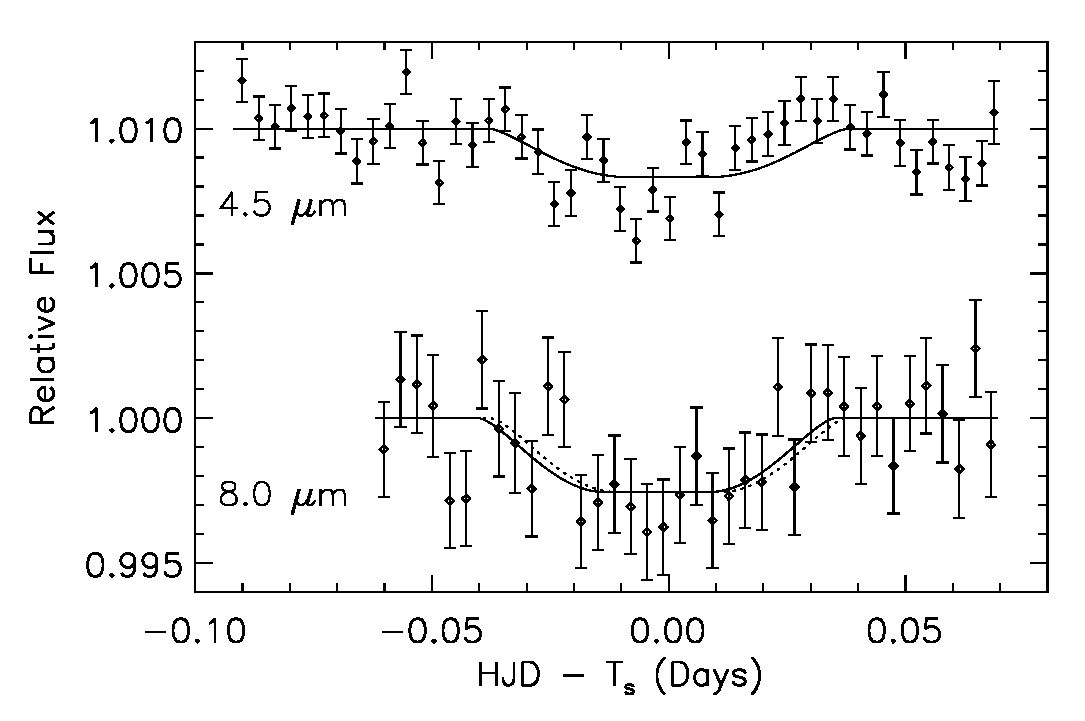
\includegraphics[width=0.95\textwidth]{6_f1}
\caption[%
Near-infrared relative fluxes from TrES-2 from {\it Spitzer} observations]{%
Relative fluxes from the TrES-2 system at 8.0\,$\mu$m ({\it bottom}) and at 4.5\,$\mu$m ({\it top}, with an arbitrary flux offset), binned and plotted versus the time from the predicted center of secondary eclipse ($T_{s}$).
Superimposed are our best-fit models (\emph{black lines}) with depths of \mbox{$\Delta f_{\rm {4.5}} = 0.00168 \pm 0.00022$} and \mbox{$\Delta f_{\rm {8.0}} = 0.00253 \pm 0.00045$}, respectively.
The timing of the secondary eclipse was allowed to vary for the 8.0-$\mu$m data (but not for the 4.5-$\mu$m data), and the derived timing offset (\mbox{$\Delta t_{\rm {8.0}} = -3.6^{+5.8}_{-4.4}$\,minutes}) is consistent with eclipse occurring at the predicted $T_{s}$.
The \emph{dotted line} represents a model with the same depth as our best-fit model of the 8.0-$\mu$m data, but with zero timing offset.%
}
\label{cha:spitzer:fig:tres2_combplot}
\end{center}
\end{figure}

The 8.0-$\mu$m data showed an overall increase in flux with time, but the first 32 minutes of data displayed a steeper slope.
We excluded this initial data and large flux outliers from further analysis.
In order to remove the trend, we computed a linear fit to the out-of-eclipse data, and then divided the data set by this model.
In order to extract the depth and epoch of the secondary eclipse, we created a model using the eclipse light curve code for a uniform source from \citet{Mandel_Agol:apjl:2002a}, allowing the eclipse depth ($\Delta f_{\rm {8.0}}$) and the offset ($\Delta t_{\rm {8.0}} $) from the predicted eclipse epoch (\mbox{$\mathrm{HJD}\,2,\!454,\!070.04823\pm0.00030$}) to vary.
The required system parameters were the planetary orbital period, impact parameter and orbital inclination (\mbox{$P=2.47063$\,days}, \mbox{$b=0.84$}; \citealt{ODonovan_Charbonneau_Mandushev:apjl:2006a} [see chapter~\ref{cha:tres2}], and \mbox{$i=83.9\degr$} \citealt{Holman_Winn_Latham:apj:2007a}), and the radius ratio between the planet and the star (\mbox{$R_{\rm p}/R_{\star}=0.1251$};  \citealt{Holman_Winn_Latham:apj:2007a}).
For each pair ($\Delta f_{\rm {8.0}}$, $\Delta t_{\rm {8.0}}$) over the range($0.0005 \le \Delta f_{\rm 8.0} \le 0.0040$, $-40\,\mathrm{minutes} \le \Delta t_{\rm {8.0}} \le 40\,\mathrm{minutes}$), we computed the $\chi^{2}$ of the corresponding model to the 8.0-$\mu$m data, again excluding large flux outliers.
The best-fit values were an eclipse depth of $\Delta f_{\rm {8.0}} = 0.00253 \pm 0.00045$ and a timing offset of $\Delta t_{\rm {8.0}} = -3.6^{+5.8}_{-4.4}$\,minutes, where the negative sign in time corresponds to an early secondary eclipse.
Thus we see that the best-fit timing offset is consistent with the predicted epoch for the secondary eclipse.
Figure~\ref{cha:spitzer:fig:tres2_combplot} shows this best-fit model, superimposed with the 8.0-$\mu$m data binned using 7-minute bins.
The reduced $\chi^{2}$ for this fit was:
\begin{eqnarray*}
\chi_{\rm r}^{2} & = & \chi^{2}/(N-2), \\
 & = & 857.4/(852-2), \\
 & = & 1.01,
\end{eqnarray*}
corresponding to a well-fit data set.

An upper limit for the orbital eccentricity of a transiting planet can be computed from the timing offset $\Delta t_{\rm {8.0}}$ derived above, using $e \, \cos{\omega} \simeq \pi \, \Delta t_{\rm 8.0}/2 \, P$, where $\omega$ is the unknown longitude of periastron and $P$ is the known orbital period (\citealp[see equation~4 of][]{Charbonneau_Allen_Megeath:apj:2005a}).
This upper limit for \tresTwo\ is therefore \mbox{$0.00145\pm0.00096$}, consistent with a negligible orbital eccentricity.
Spitzer has also obtained a negligible orbital eccentricity for two other planets: \hdTZNb\ \citep{Deming_Seager_Richardson:nat:2005a} and \tresOne\ \citep{Charbonneau_Allen_Megeath:apj:2005a}.
Tidal damping of orbital eccentricity (Bodenheimer, Lin, \& Mardling~\citeyear{Bodenheimer_Lin_Mardling:apj:2001a}; Bodenheimer, Laughlin, \& Lin~\citeyear{Bodenheimer_Laughlin_Lin:apj:2003a} has yet to be shown to be a sizable contribution to the internal energy of any exoplanet.

The analysis of the 4.5-$\mu$m data was complicated by the known correlation between the IRAC 4.5-$\mu$m flux from a source and the intra-pixel position on the detector.
For this data set, we assumed the eclipse occurred at the predicted time (consistent with the above 8.0-$\mu$m timing offset for this secondary eclipse), and measured the eclipse depth at this wavelength.
Here we excluded outliers not only in flux, but also in $x$ or $y$ position.
Our model consisted of the product of a model eclipse light curve
and a second-order polynomial in $x$ and $y$.
Again, we minimized the $\chi^{2}$ of our model fit to the 4.5-$\mu$m data, this time using the AMOEBA algorithm \citep{Press_Teukolsky_Vetterling:1992a}.
The derived 4.5-$\mu$m eclipse depth was \mbox{$\Delta f_{\rm {4.5}} = 0.00168 \pm 0.00022$}.
The reduced $\chi^{2}$ for this fit was \mbox{$\chi_{\rm r}^{2} = 798.8/(1051-1)=0.76$}, corresponding to a well-fit data set.
In figure~\ref{cha:spitzer:fig:tres2_combplot}, we show our binned 4.5-$\mu$m data, together with our best-fit theoretical light curve.

\section{Atmospheric Models for TrES-2}
\label{cha:spitzer:sec:atm}

\begin{figure}
\begin{center}
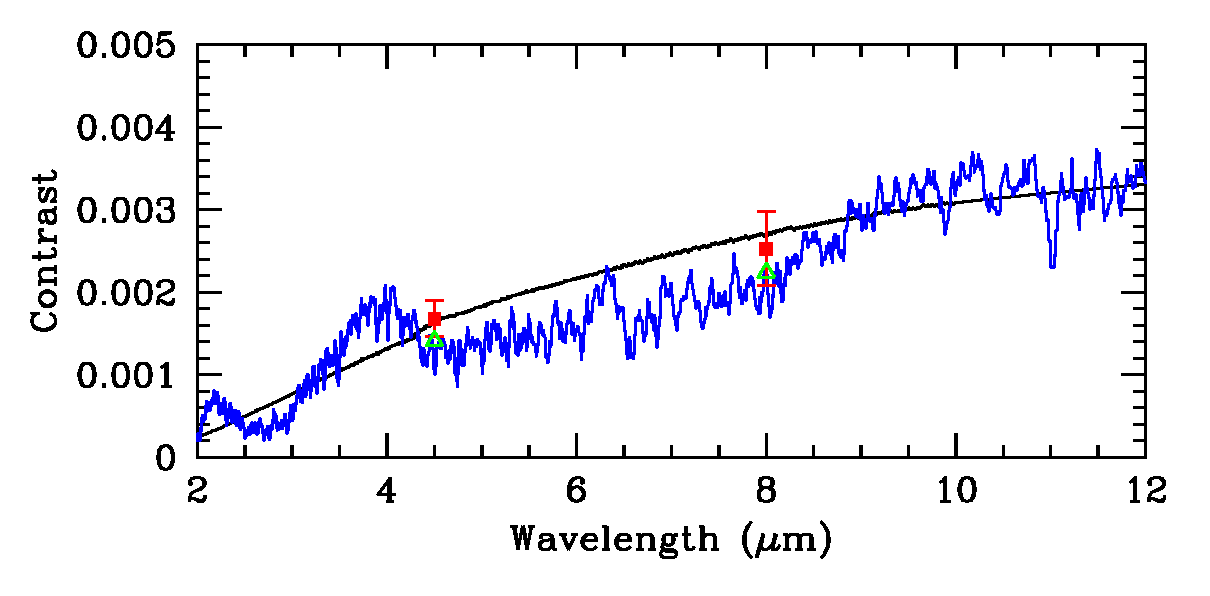
\includegraphics[width=0.95\textwidth]{6_f2}
\caption[%
Near-infrared contrast ratios for TrES-2]{%
Contrast ratios ({\it red squares}) for TrES-2 at 4.5\,$\mu$m and 8.0\,$\mu$m, which are consistent with a model ({\it black line}) of a 1450\,K blackbody planetary flux divided by a Kurucz model of the star TrES-2. Also shown are the predictions ({\it green triangles}) for these fluxes from a theoretical planet-star flux contrast model ({\it blue line}) computed for the star TrES-2 using the \citet{Seager_Richardson_Hansen:apj:2005a} code (see text).%
}
\label{cha:spitzer:fig:tres2models}
\end{center}
\end{figure}

We now turn to a discussion of the \tresTwo\ 4.5-$\mu$m and 8.0-$\mu$m planet-star contrast.
We first emphasize how well the data are fit by a blackbody spectrum of 1450\,K.
The {\it black line} in figure~\ref{cha:spitzer:fig:tres2models} is a 1450\,K blackbody flux divided by a Kurucz stellar model appropriate for the stellar parameters derived by \citet{Sozzetti_Torres_Charbonneau:apj:2007a}.
A blackbody of 1450\,K implies a Bond albedo of 0.12, with the assumption of uniform redistribution of absorbed stellar radiation.
If \tresTwo\ is indeed a blackbody, it would add to the growing list of published hot Jupiter atmosphere data commensurate with blackbody spectra, showing no evidence for the atmospheric composition.
These exoplanets include two of the three exoplanets with more than one published data point: \tresOne\ \citep{Charbonneau_Allen_Megeath:apj:2005a} and the \hdOENb\ spectrum \citep{Grillmair_Charbonneau_Burrows:apjl:2007a}.
A theoretical planet-star flux contrast that fits the data is also shown as the {\it blue line} in figure~\ref{cha:spitzer:fig:tres2models}.
The \tresTwo\ spectrum was generated from a model atmosphere code for hot Jupiters \citep{Seager_Richardson_Hansen:apj:2005a} with inputs appropriate to the \tresTwo\ planet-star parameters, solar abundances, and a Kurucz model atmosphere for the irradiation from the parent star.
We reduce the incident stellar flux by \mbox{$f=0.9$} to take into account the redistribiution of absorbed stellar radiation.
This value is intermediate between the values for instantaneous reradiation (\mbox{$f=3/8$}) and uniform redistribution (\mbox{$f=1$}) of absorbed stellar radiation.
The planet spectrum has \mbox{$T_{\rm eff}=1550$\,K}.
Planets with higher values of $f$ (i.e., under the assumption that the absorbed stellar radiation is redistributed more uniformly) than the one we chose have flux values too low in both the 4.5-$\mu$m and 8.0-$\mu$m bandpasses.
We justify our somewhat arbitrary choice of $f$ based on the results of \citet{Fortney_Cooper_Showman:apj:2006a} that 1-D models do not represent the 3-D dayside temperature pressure profiles that likely result from a highly complex atmospheric circulation.

\section[Searching for Evidence of Atmospheric Absorption]{Searching for Evidence of Atmospheric \\ Absorption}
\label{cha:spitzer:sec:discuss}

The \spi\ data we report for \tresTwo\ is markedly different than for \tresOne\ \\ \citep{Charbonneau_Allen_Megeath:apj:2005a}.
In comparing the \tresTwo\ and \tresOne\ data sets with each other and with models, it is useful to define a \spi\ IRAC color index: the ratio of the 8.0-$\mu$m to 4.5-$\mu$m planet-star flux contrast.
For \tresOne\ the color index is \mbox{$3.41 \pm 0.87$}.
This ratio was too high to fit most atmosphere models in the literature (\citealp[see][]{Fortney_Marley_Lodders:apjl:2005a, Seager_Richardson_Hansen:apj:2005a, Barman_Hauschildt_Allard:apj:2005a};  but cf \citealt*{Burrows_Sudarsky_Hubeny:apj:2006a}).
Although many different models (including such effects as high metallicity, energy deposition at high alitudes in the atmosphere; varying C/O ratios, energy redistribution parametrizations) have since been explored (\citealp{Barman_Hauschildt_Allard:apj:2005a}; \citealp{Fortney_Marley_Lodders:apjl:2005a}; \citealp{Seager_Richardson_Hansen:apj:2005a};  Burrows, Sudarsky, \& Hubeny \citeyear{Burrows_Sudarsky_Hubeny:apj:2006a}), none reach the \tresOne\ value of 3.4.

\tresTwo\ has a much lower color index (\mbox{$1.51 \pm 0.33$}) than \tresOne.
This value is much more easily fit by ``generic'' hot Jupiter atmosphere models.
Indeed, a wide variety of theoretical models with solar abundances, with uniform or hemispheric redistribution, with or without clouds, and for a wide range of temperatures and redistribution values, have ratios consistent with the \tresTwo\ color index \citep[see, e.g.,][]{Fortney_Marley_Lodders:apjl:2005a, Barman_Hauschildt_Allard:apj:2005a, Charbonneau_Allen_Megeath:apj:2005a}.
This is primarily because the water vapor absorption features in these models dominate the spectra, and appears to create a somewhat consistent color index.

\spi\ IRAC data at 3.6\,$\mu$m and 5.8\,$\mu$m are forthcoming for \tresTwo.
These additional data are critical to distinguish between a blackbody spectrum, a radiative equilibrium solar abundance spectrum, and other atmosphere models.


% chktex-file 44
\chapter[Identifying Transits in TrES Data Sets: The Human Factor]%
{%
Identifying Transits in \\ TrES Data Sets: \\ The Human Factor%
\protect\CFNF%
}\label{cha:human}

\section{Understanding the Yield of Transit Surveys}\label{cha:human:sec:intro}

The discovery of the first transiting planet \hdTZNb\ \citep{Charbonneau_Brown_Latham:apjl:2000a, Henry_Marcy_Butler:apj:2000a} spawned a great flurry of campaigns to search for these rare objects.
Transiting planets yield precise measurements of the radius and mass of giant planets outside our solar system that are much needed constraints for theoretical models, and they provide the promise of a better understanding of the structure and formation of gas giants.
\hdTZNb\ was first identified \citep{Mazeh_Naef_Torres:apj:2000a} as a Jupiter-mass planet by radial-velocity surveys of the solar neighborhood.
It was later observed to transit its star.
In comparison, the majority of transit surveys aimed to photometrically monitor $100,\!000$s of stars for evidence of transits.
Initial estimates \citep[see, e.g.,][]{Horne:ASP:2003a} of the yield of transiting planets from these surveys were optimistic during the initial rush of enthusiasm, with expectations of many new discoveries every month.
At the time of writing, seven years later, there are only 20 known transiting exoplanets.
Several transit surveys have overcome the difficulty in obtaining the photometric precision required to observe a 1\% transit over a large field of view for thousands of stars, and have proven their ability to identify transiting planets: the OGLE-III survey \citep{Udalski_Paczynski_Zebrun:acta:2002a}, the XO project \citep{McCullough_Stys_Valenti:pasp:2005a}, the HAT survey \citep{Bakos_Lazar_Papp:pasp:2002a}, the SuperWASP survey \citep{Street_Pollaco_Fitzsimmons:ASP:2003a}, and the Trans-atlantic Exoplanet Survey (TrES;\@\citealt{Alonso_Deeg_Brown:an:2004a, Dunham_Mandushev_Taylor:pasp:2004a, ODonovan_Charbonneau_Kotredes:AIP:2004a}).
Despite these successes, the anticipated flood of new transiting planets is still only a trickle.

Over time, we have developed a greater appreciation of additional factors that must be included in our predictions \citep[see][for a review]{Gaudi:asp:2007a}:
(i) Transit surveys are very biased toward large planets with short periods (Gaudi, Seager, \& Mallen-Ornelas~\citeyear{Gaudi_Seager_Mallen-Ornelas:apj:2005a}; \citealp{Gaudi:apjl:2005a}).
(ii) Many of the stars in a given field are giants or large dwarfs \citep{Brown:apjl:2003a}; hence transits of these large stars are not detectable by ground-based surveys with ten-centimeter telescopes.
(iii) The presence of systematics in the data, correlated on transit-like time scales, increases the signal-to-noise ratio requirement to detect a transit to beyond that derived from simple Poisson noise.
This increases the number of observed transits required to have a strong transit detection, and hence affects the choice of the length of the observing run for the field.

These factors affect the number of strong transit signals that are expected in the data.
However, when estimating the yield from a survey, we must account for how we detect these periodic signals.
There are two steps in my procedure for identifying candidate transiting systems.
First, I use an automated algorithm to find the statistically most significant transit signals.
Then, I view these strong signals and determine which are worth further analysis.
It is important that both steps are efficient in recovering transit signals.
Several algorithms have been proposed in the case of transit surveys \citep[see, e.g.,][for a review]{Tingley:aa:2003a, Tingley:aa:2003b}.
For the analysis of the TrES data, I use the Box-fitting Least-Squares (BLS) transit-search algorithm of \citeauthor*{Kovacs_Zucker_Mazeh:aa:2002a}~(\citeyear{Kovacs_Zucker_Mazeh:aa:2002a}, see appendix~\ref{cha:bls}), as do several other groups such as the HAT survey.
Several studies of the potential recovery rates of transit candidates have been done by transit surveys \citep[see, e.g.,][]{Gilliland_Brown_Guhathakurta:apjl:2000a, Bramich_Horne_Bond:mnras:2005a, Kane_Collier-Cameron_Horne:mnras:2005a, Weldrake_Sackett:apj:2005a}.
Here I present the recovery rate of the BLS algorithm when applied to TrES data.
I also discuss my ability to spot true transit signals among the noise, as the efficiency of this step has not been previously quantified.

\section[Injecting Model Light Curves into a TrES Data Set]{Injecting Model Light Curves into a \\ TrES Data Set}\label{cha:human:sec:model}

I conducted a blind test of my ability to identify transit-like signals in a real data set from the TrES campaign.
I chose the TrES Lyr1 field (centered on the star \mbox{16\,Lyr}) in which I had identified the transiting planet \tresTwo\ (\citealp{ODonovan_Charbonneau_Mandushev:apjl:2006a}, see chapter~\ref{cha:tres2}).
The total yield to date of this $5.7\degr \times 5.7\degr$ field, which contains 27,446 stars, is one confirmed planet.

\begin{figure}
\begin{center}
\centering
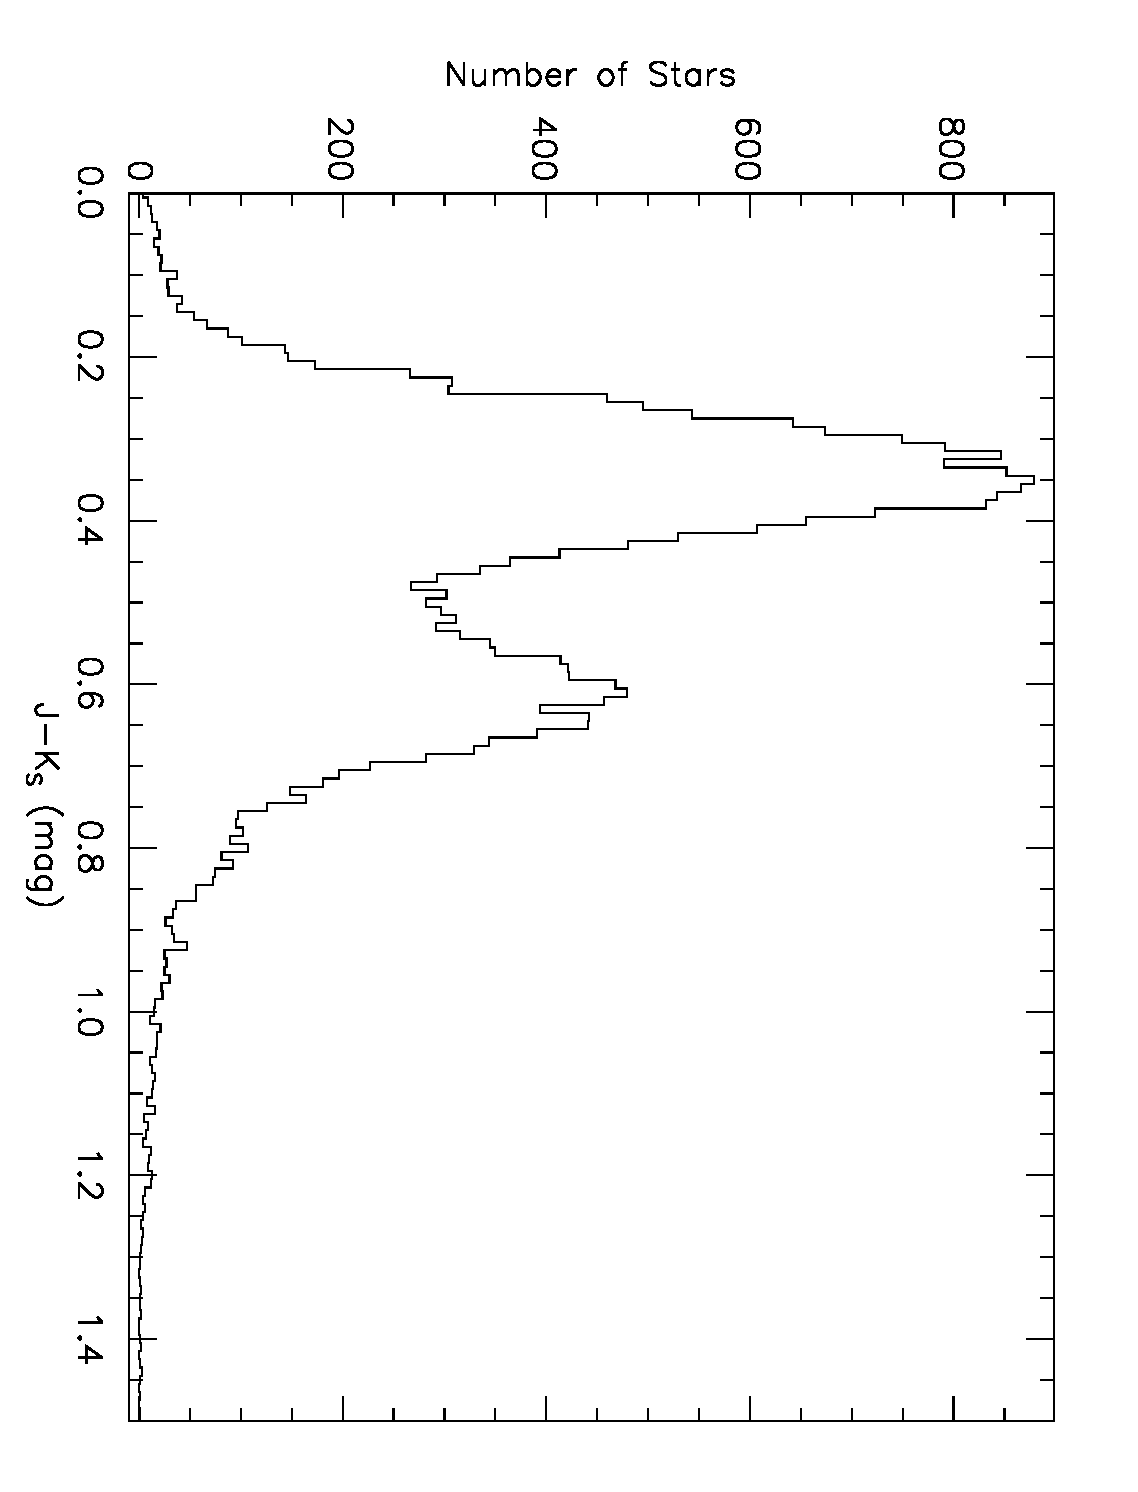
\includegraphics[width=.75\textwidth, angle=90]{7_jmks}\\
\caption[Histogram of 2MASS $J-K_{s}$ for TrES Lyr1 field]{%
Histogram of the 2MASS $J-K_{s}$ infrared colors for the TrES Lyr1 field.%
}\label{cha:human:sec:model:fig:jmks}
\end{center}
\end{figure}

\begin{figure}
\begin{center}
\centering
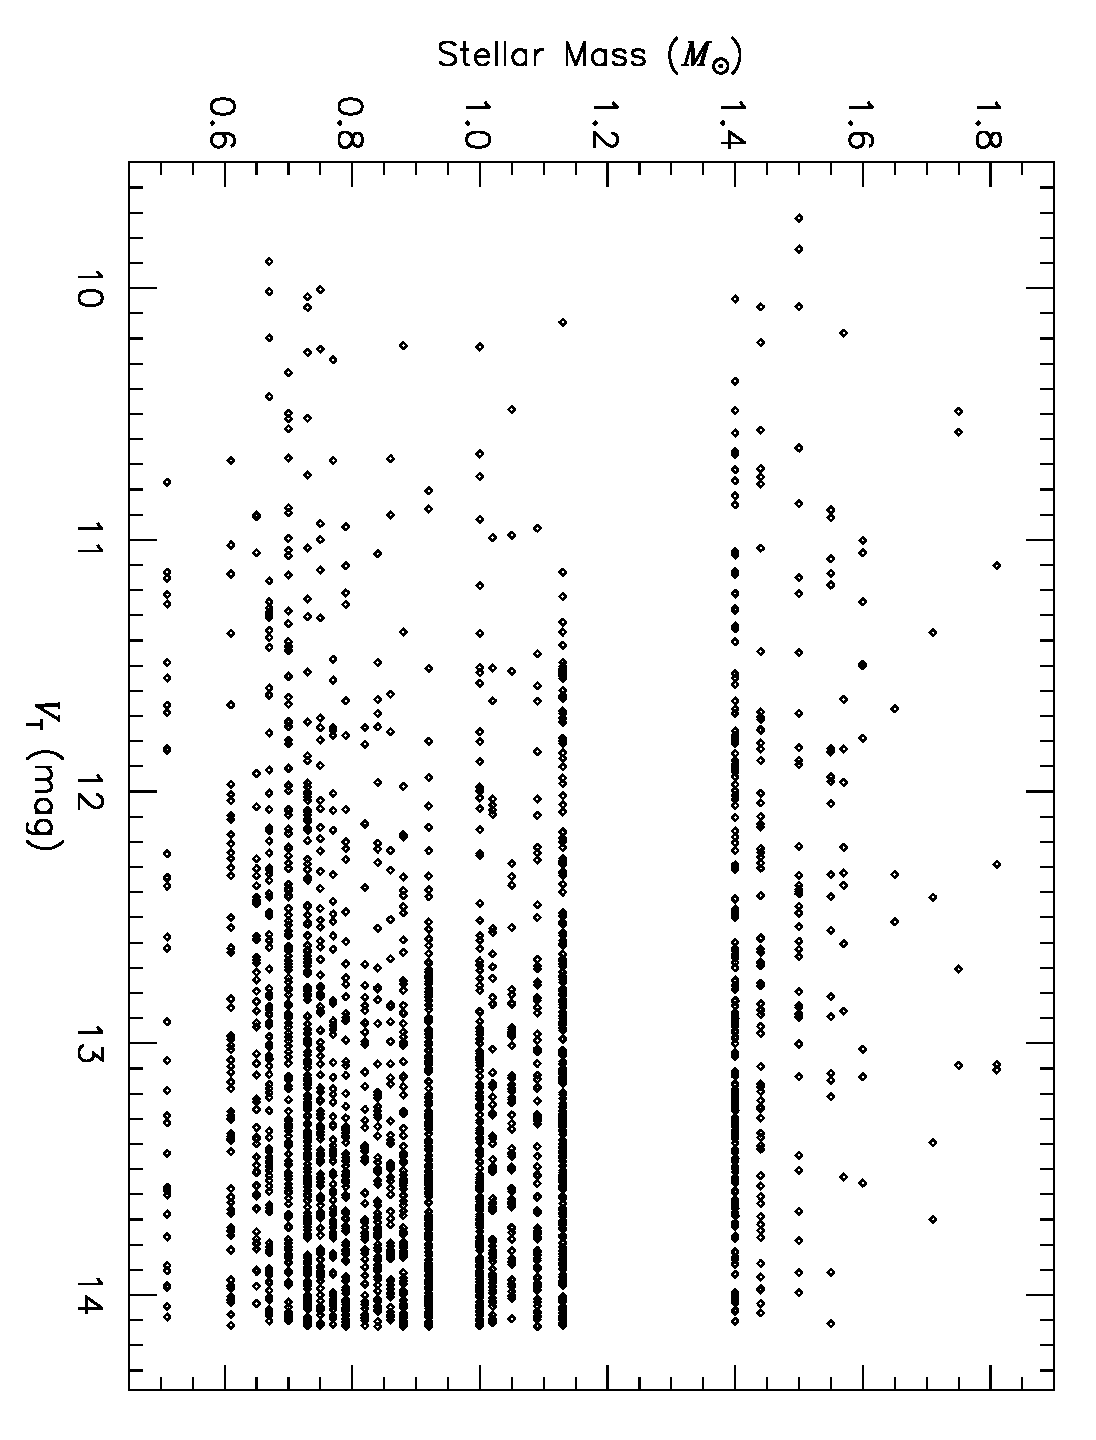
\includegraphics[width=.60\textwidth, angle=90]{7_phys_a}\\
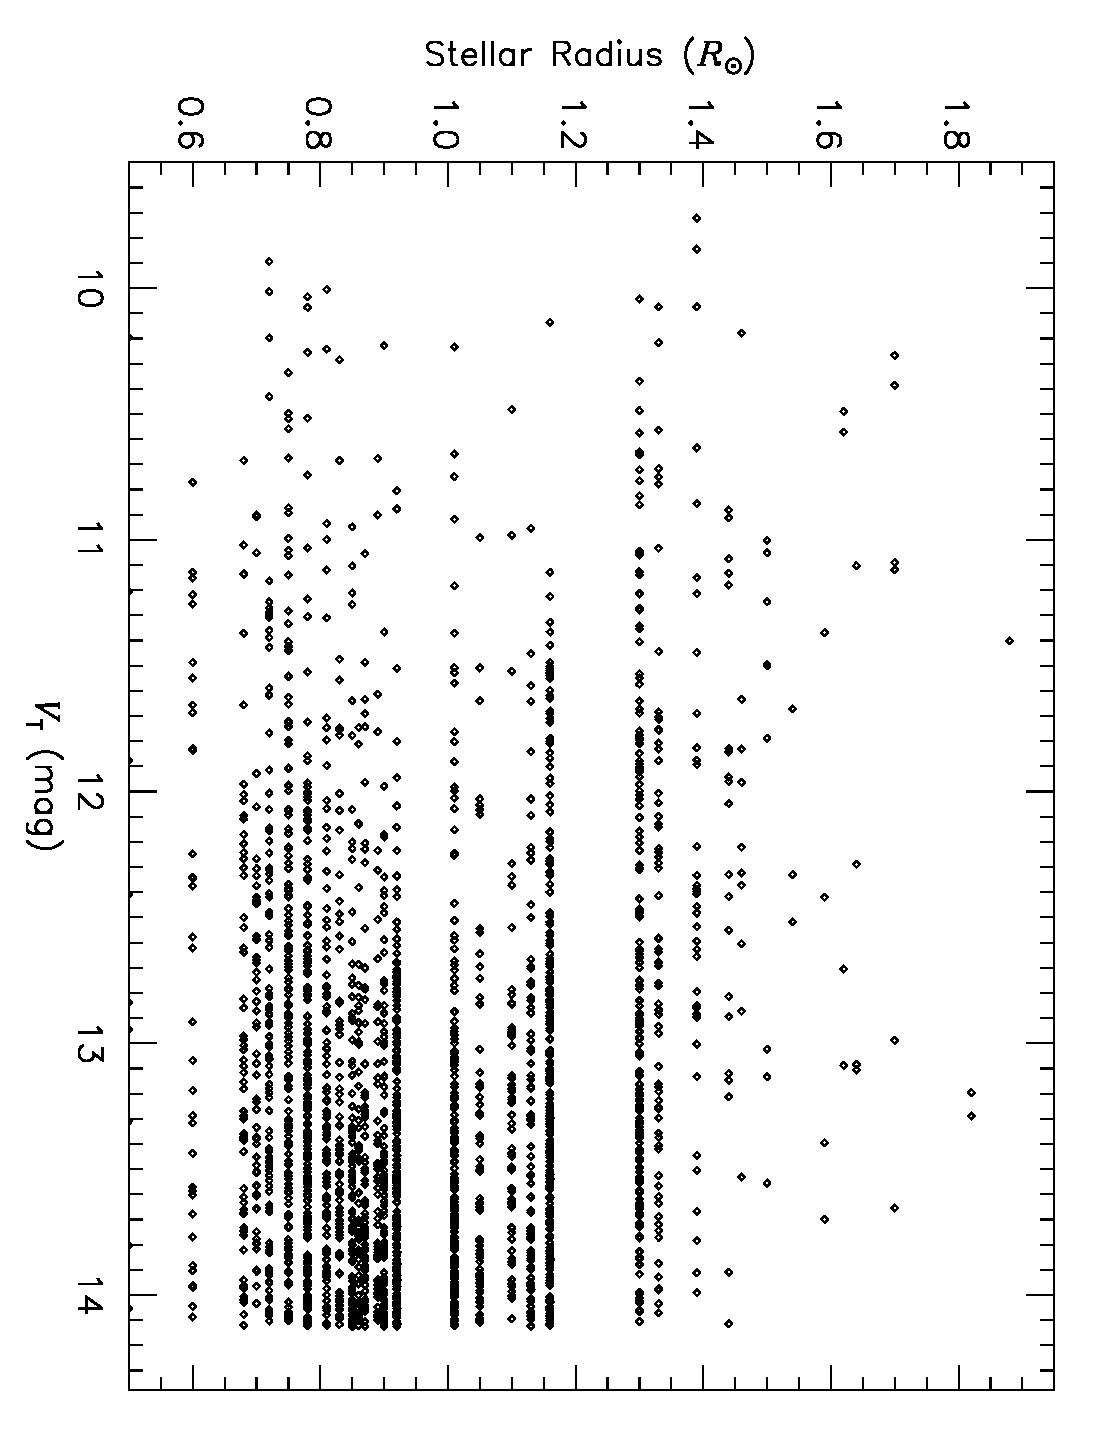
\includegraphics[width=.60\textwidth, angle=90]{7_phys_b}\\
\caption[Randomized stellar parameters for injected transits]{%
Randomized stellar parameters used to generate fake transit light curves injected into a TrES time series, plotted versus the approximate $V_{T}$ magnitudes: %
({\textit top panel}) the mass of the host star, and %
({\textit bottom panel}) the stellar radius.
The number of stars of a given magnitude increases with magnitude.
The stellar mass and radius were generated using the 2MASS $J-K_{s}$ infrared colors from figure~\ref{cha:human:sec:model:fig:jmks} (see text for a discussion of the distribution).
These values were computed to two decimal places, which results in the discrete levels visible in the plots.%
}\label{cha:human:sec:model:fig:stel}
\end{center}
\end{figure}

\begin{figure}
\begin{center}
\centering
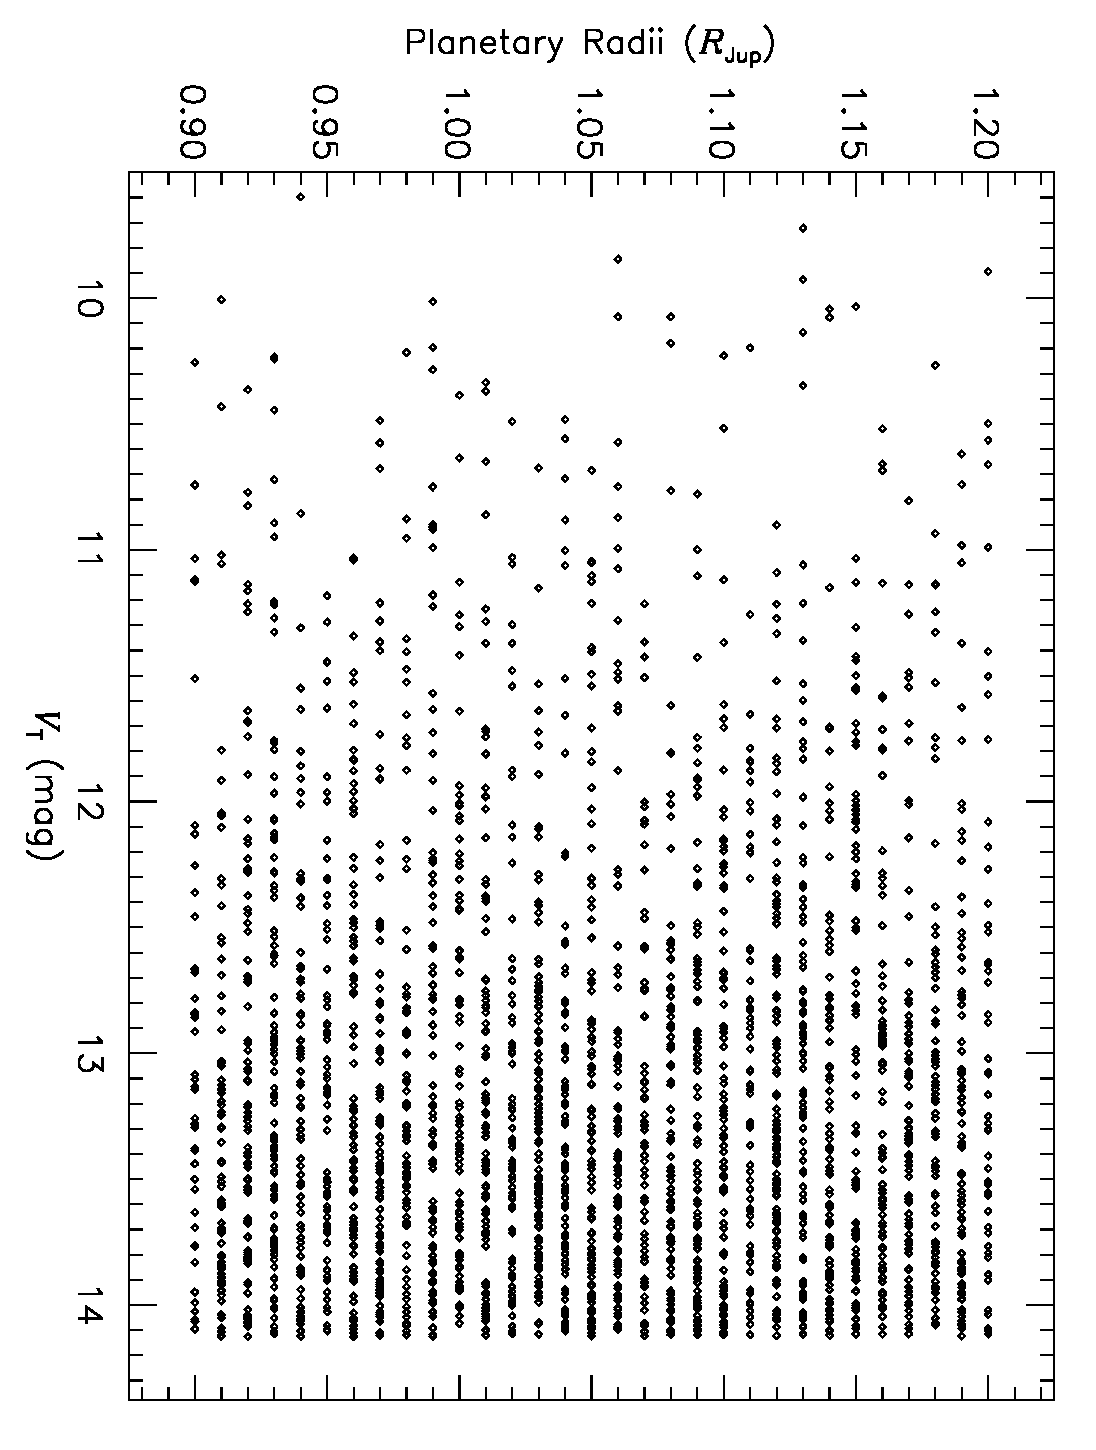
\includegraphics[width=.75\textwidth, angle=90]{7_phys_c}\\
\caption[Randomized planetary parameters for injected transits]{%
Same as for figure~\ref{cha:human:sec:model:fig:stel}, but for the radius $R_{p}$ of the supposed transiting planet.
Again, the discrete levels in the values for $R_{p}$ are due to the limit of two decimal places for the values.
%
}\label{cha:human:sec:model:fig:plan}
\end{center}
\end{figure}

First I generated a list of parameters for fake transit light curves as follows.
Note that I did not consult this parameter list until I had attempted to visually identify all of the fake candidate transiting planets.
As part of the standard TrES analysis pipeline (\citealp[see, e.g.,][]{Dunham_Mandushev_Taylor:pasp:2004a}; \citealp{ODonovan_Charbonneau_Torres:apj:2006a}, see chapter~\ref{cha:gsc}; \citealp{ODonovan_Charbonneau_Alonso:apj:2007a}, see chapter~\ref{cha:and0}).% chktex 9 chktex 10
I had previously generated a list of 27,446 stars present in the Lyr1 field, ordered by instrumental $r$ magnitude.
The position of a star in this list, starting at 0 for the brightest star, is the ``star number'' for this star.
In order to span a wide range of transit parameters, I would need to inject a large number of fake transits.
However, I would also need to somewhat simulate the scarcity of real transit signals in the data.
I decided to choose a random%
\footnote{%
The random numbers discussed in this chapter were generated using IDL's \textit{RANDOMU} function that generates uniformly distributed, pseudo-random numbers using the method of~\citet{Park_Miller:ACM:1988a}.%
}%
\ number of fake transits to be injected, such that this number was $\sim$10\% of the total number of stars.
I then chose this number (2,612) of stars at random from the star list to be the ostensible candidate hosts of transiting planets.
From the 2MASS \citep{Cutri_Skrutskie_van-Dyk:2003a} $J-K_{s}$ infrared colors of these stars (see figure~\ref{cha:human:sec:model:fig:jmks}), I derived the stellar masses $M_{\star}$ and radii $R_{\star}$, assuming these to be dwarf stars and using an interpolation%
\footnote{%
The gaps in the stellar masses and radii were caused by a bug in the interpolation code that was not discovered until the hidden parameter file was examined after the analysis.
Future analysis will correct this.
However, I decided that the stellar radii (the more interesting parameter) cover a wide enough parameter space for my initial analysis.%
}%
\ of values from \citet{Cox::2000a}.
Note that since most of the stars with large $J-K_{s}$ values are in fact giants, the assumption that these stars are main-sequence stars (with small stellar radii corresponding to their color) leads to a bias toward identifying transiting planets that are too small to be detected if transiting giant stars.
The scarcity of radii $\rstar<0.65\,\rsun$ and $\rstar>1.40\,\rsun$ (and the similar dearth in masses) is the result of the 2MASS color distribution of figure~\ref{cha:human:sec:model:fig:jmks}.
I produced a random distribution of radii $R_{p}$ for the supposed planetary companions of these stars, where $0.9\leq R_{p} \leq 1.2\,R_{\mathrm Jup}$ based on the distribution of radii for the known transiting planets (see figure~\ref{cha:intro:sec:methods:sub:trans:fig:tp}).
The values for these three physical parameters are shown in figures~\ref{cha:human:sec:model:fig:stel} and~\ref{cha:human:sec:model:fig:plan}.

\begin{figure}
\begin{center}
\centering
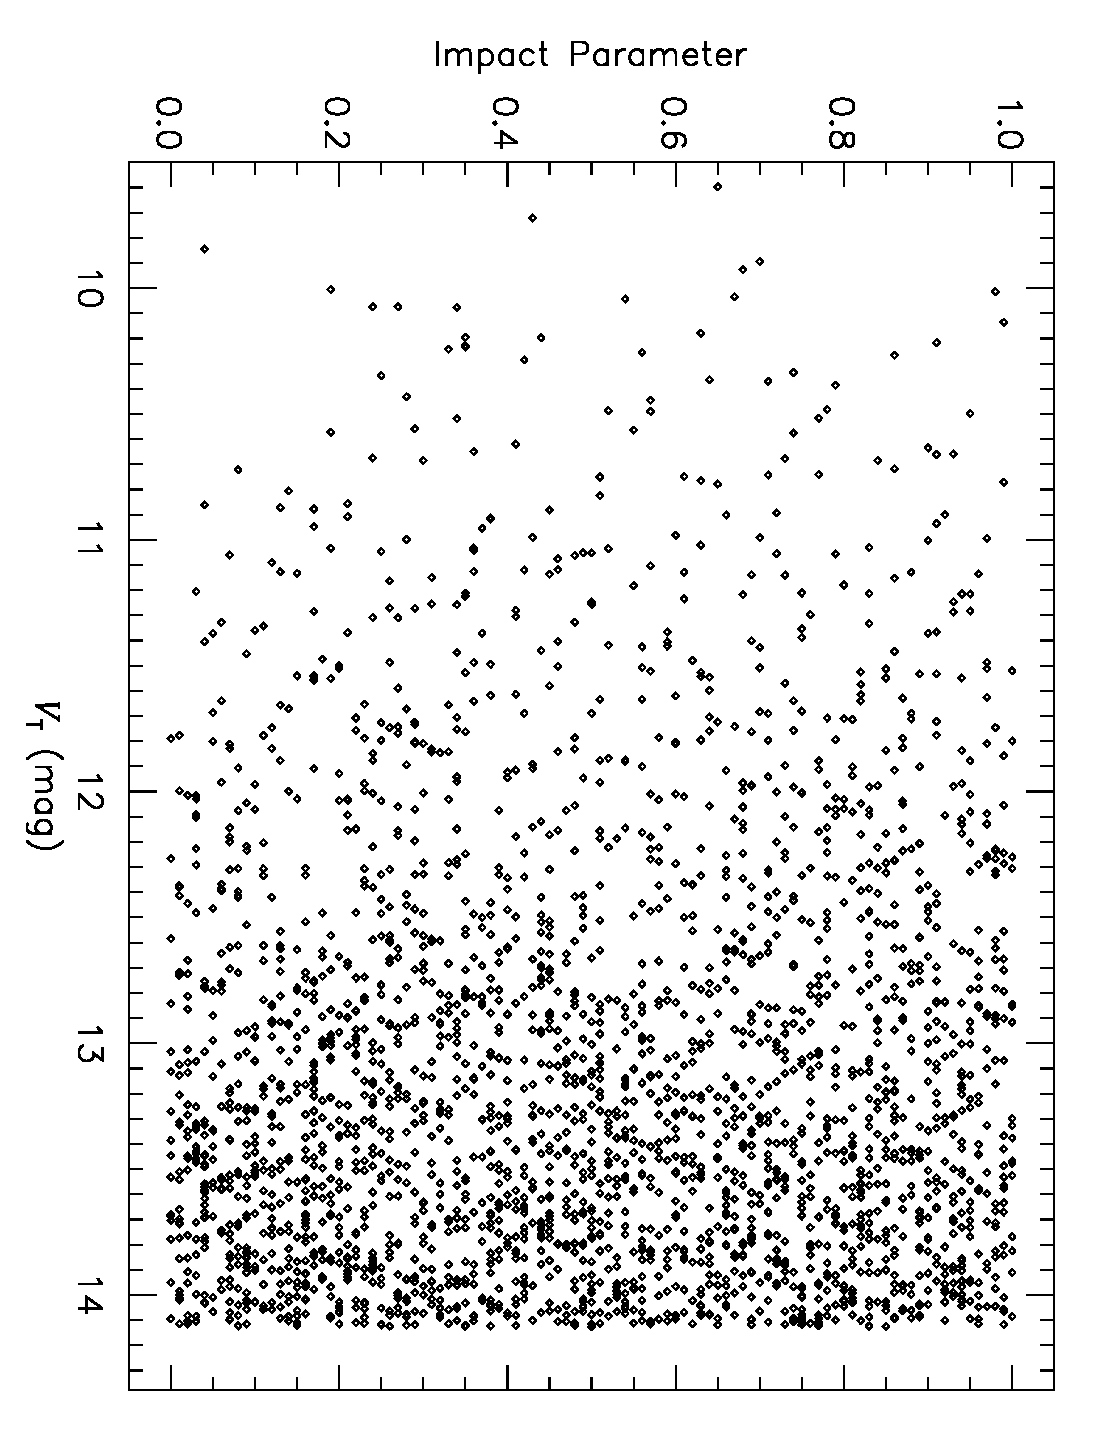
\includegraphics[width=.55\textwidth, angle=90]{7_orb_a}\\
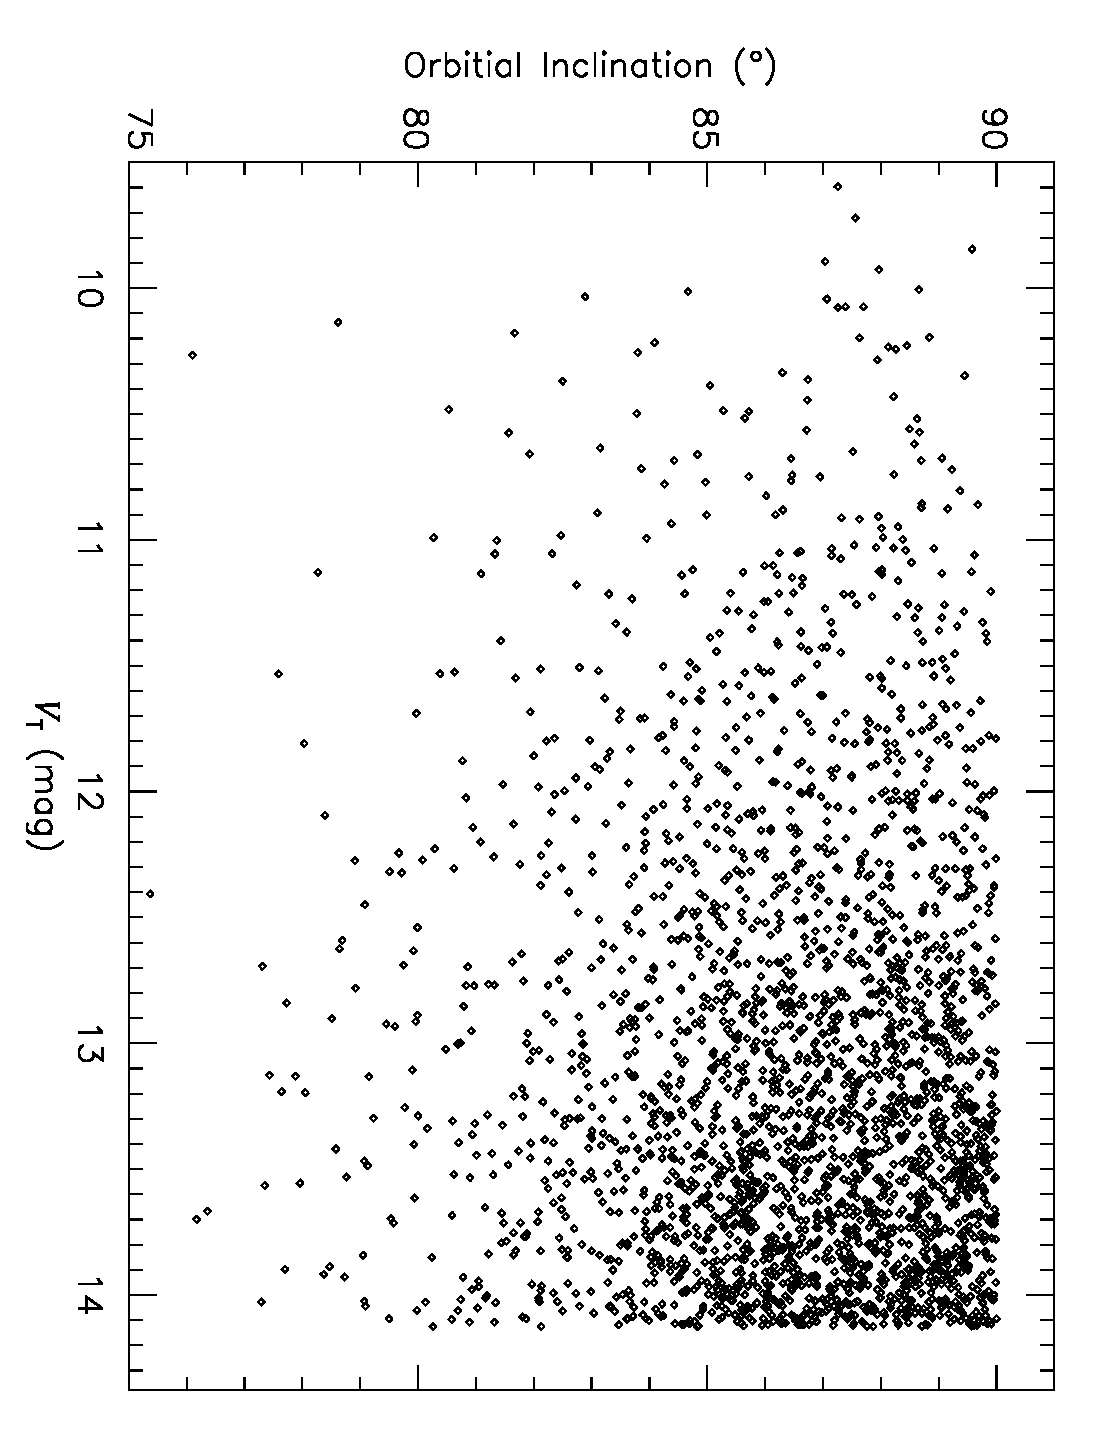
\includegraphics[width=.55\textwidth, angle=90]{7_orb_b}\\
\caption[Randomized transit impact parameters and orbital inclinations]{%
Randomized impact parameters ({\textit top panel}) for the model
transiting systems, from which the orbital inclinations in the {\textit bottom panel} are derived.
The orbital inclination is only significantly lower than $90\degr$ for those candidates with short periods and large impact parameters.
For example, if $i<80\degr$, $P=1$\,day, and $R_{\star}=R_{\sun}$, then $b$ must be greater than 0.7. %
}\label{cha:human:sec:model:fig:orb}
\end{center}
\end{figure}

I then computed random values for the transit impact parameter $b$ ($0\leq b\leq 1$).
From $b$, we can derive the orbital inclination $i= \arccos{(b R_{\star}/a)}$, where $a$ is the orbital semi-major axis computed using Newton's revised version of Kepler's third law.
The distribution of $b$ and $i$ can be seen in figure~\ref{cha:human:sec:model:fig:orb}.

\begin{figure}
\begin{center}
\centering
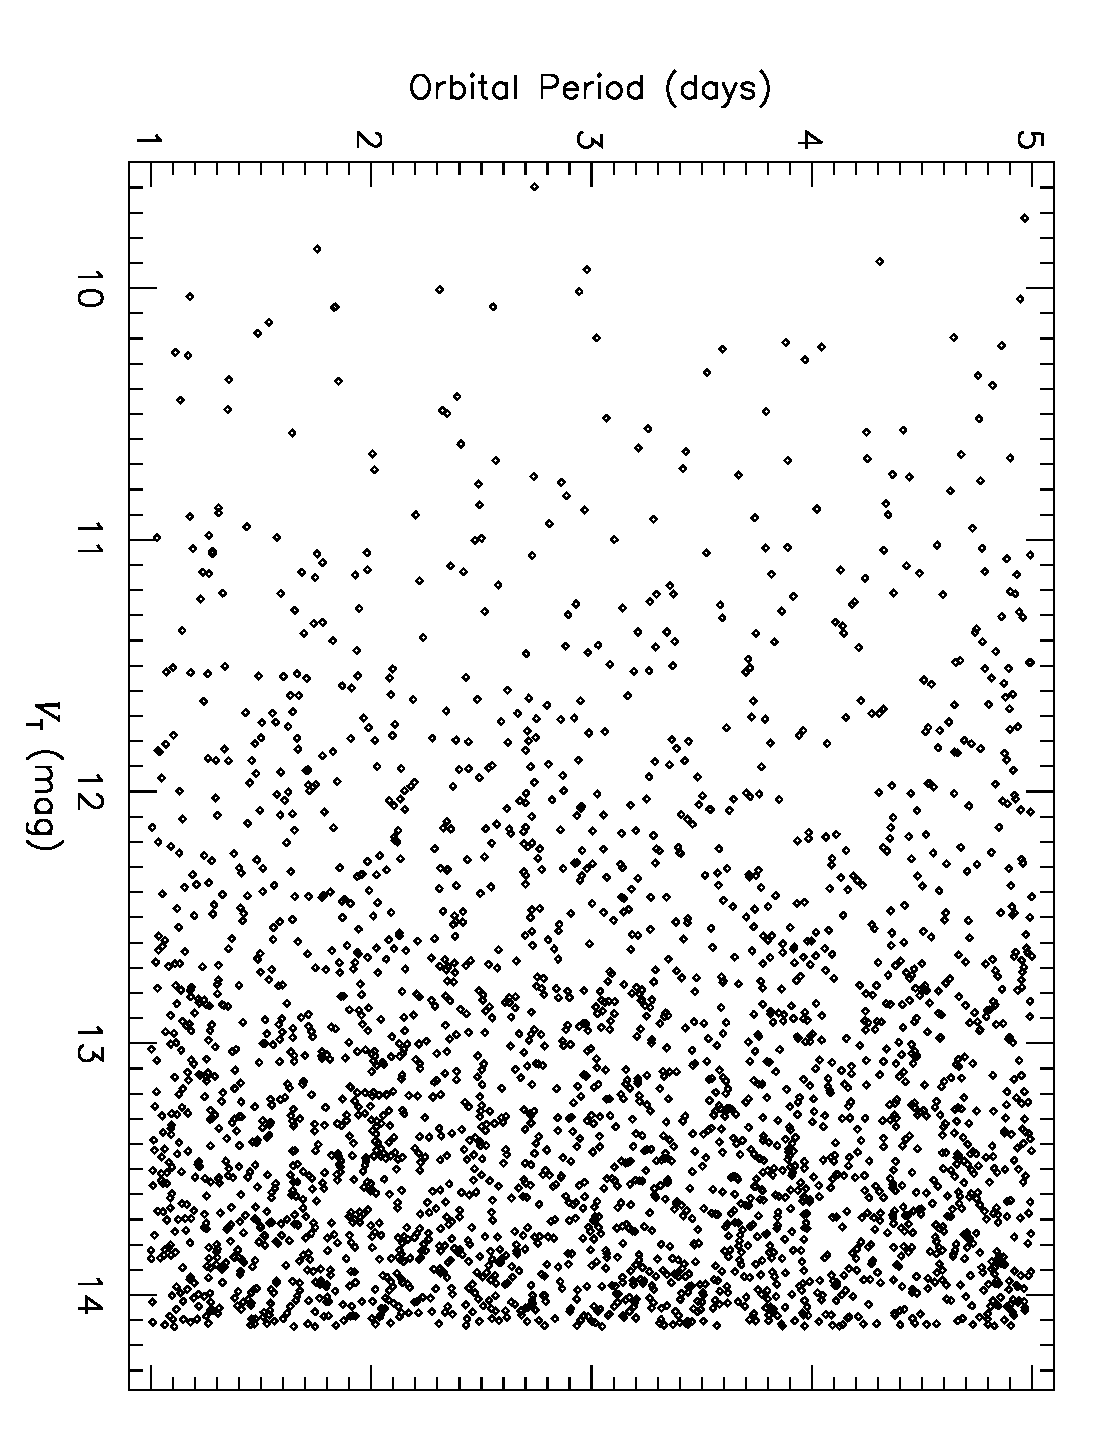
\includegraphics[width=.55\textwidth, angle=90]{7_bls_a}\\
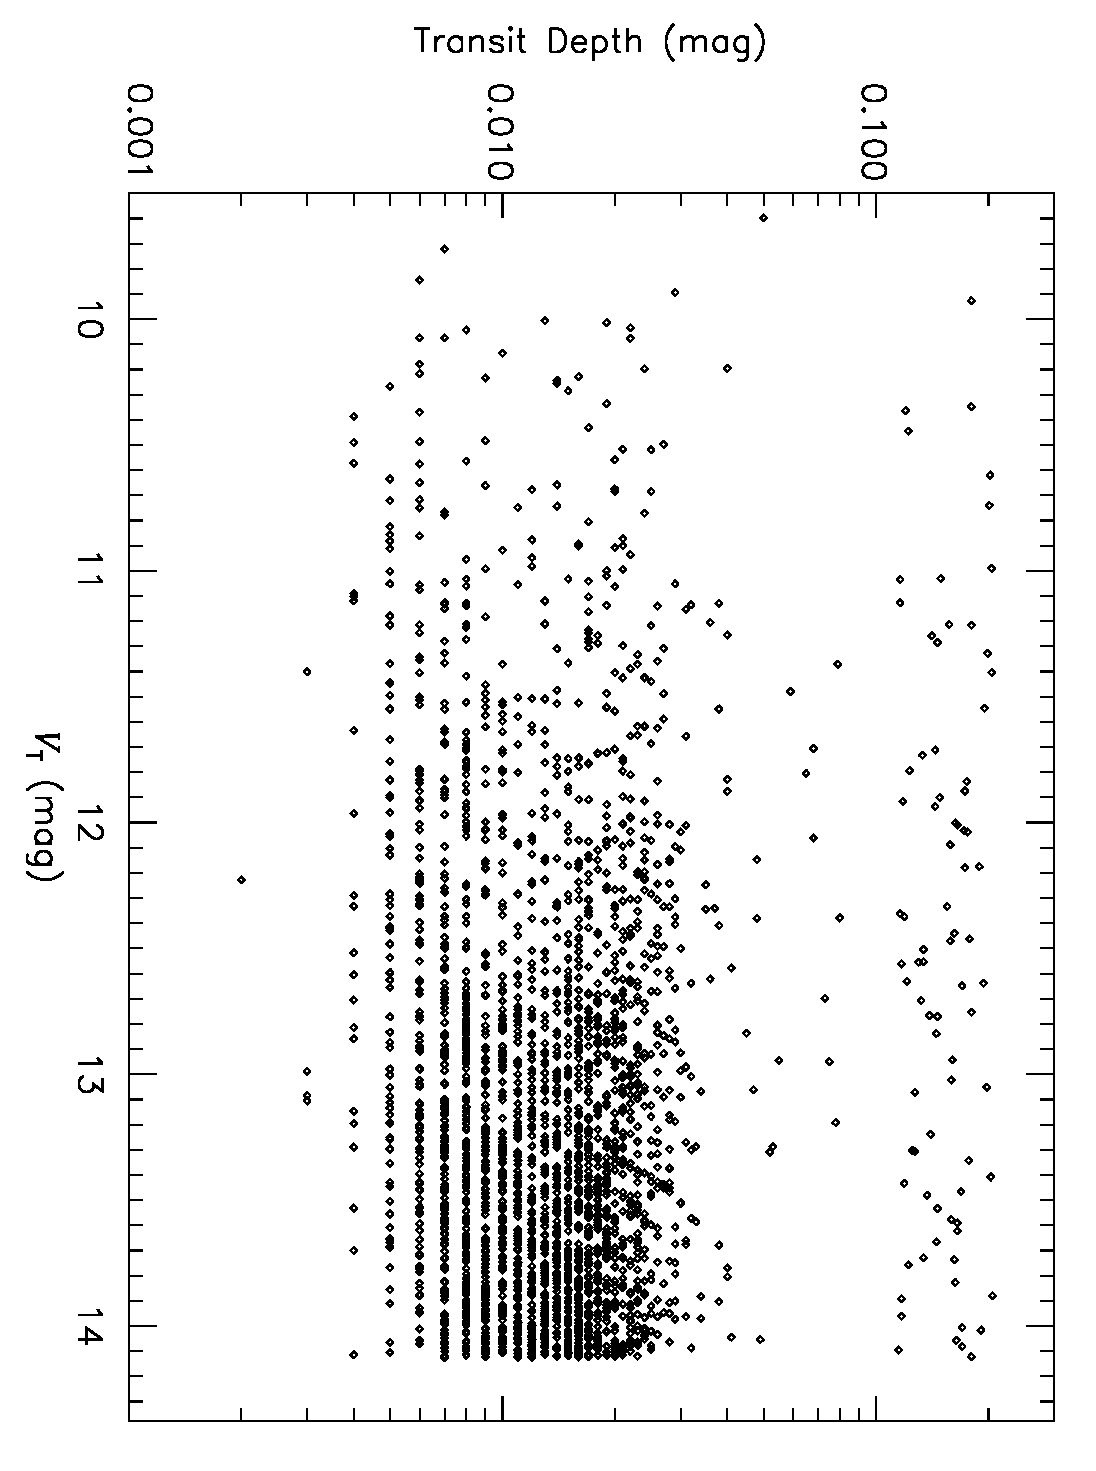
\includegraphics[width=.55\textwidth, angle=90]{7_bls_b}\\
\caption[Randomized values for first two BLS parameters]{%
Randomized values for two of the four parameters that are derived for each light curve by the Box-fitting Least-Squares (BLS) transit-search algorithm: %
({\textit top panel}) the orbital period $P$ of the transit, and %
({\textit bottom panel}) the transit depth $\Delta$.
To mimic the output of the BLS algorithm, $P$ and $\Delta$ are kept to 6 and 3 decimal places, respectively.
Since \mbox{$0.9\,\rjup \leq \rp \leq 1.2\,\rjup$} and most derived stellar radii lie in the range \mbox{$0.7\,\rsun \leq \rstar \leq 1.3\,\rsun$}, most of the transit depths are in the range \mbox{$0.005 \leq \Delta \leq 0.03$}.
The outliers are those transits of a very small star by very large planet, or of a very large star by a very small planet.
These points are evidence of the aforementioned bias caused by the assumption that all field stars are dwarf stars. %
}\label{cha:human:sec:model:fig:bls1}
\end{center}
\end{figure}

\begin{figure}
\begin{center}
\centering
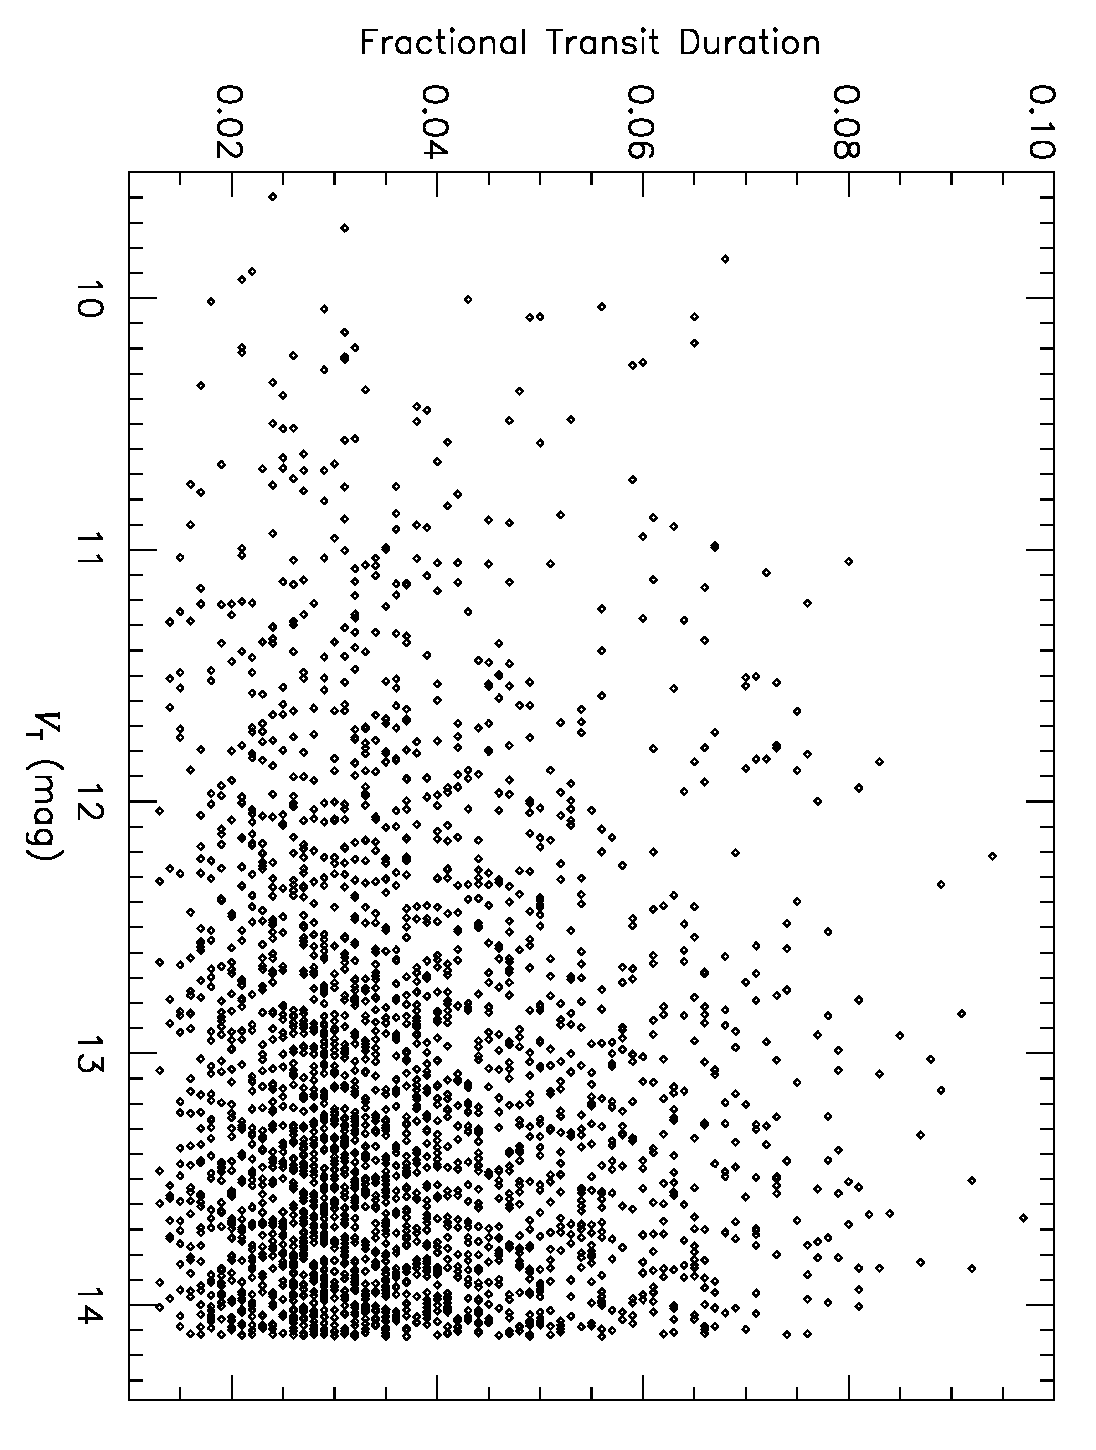
\includegraphics[width=.55\textwidth, angle=90]{7_bls_c}\\
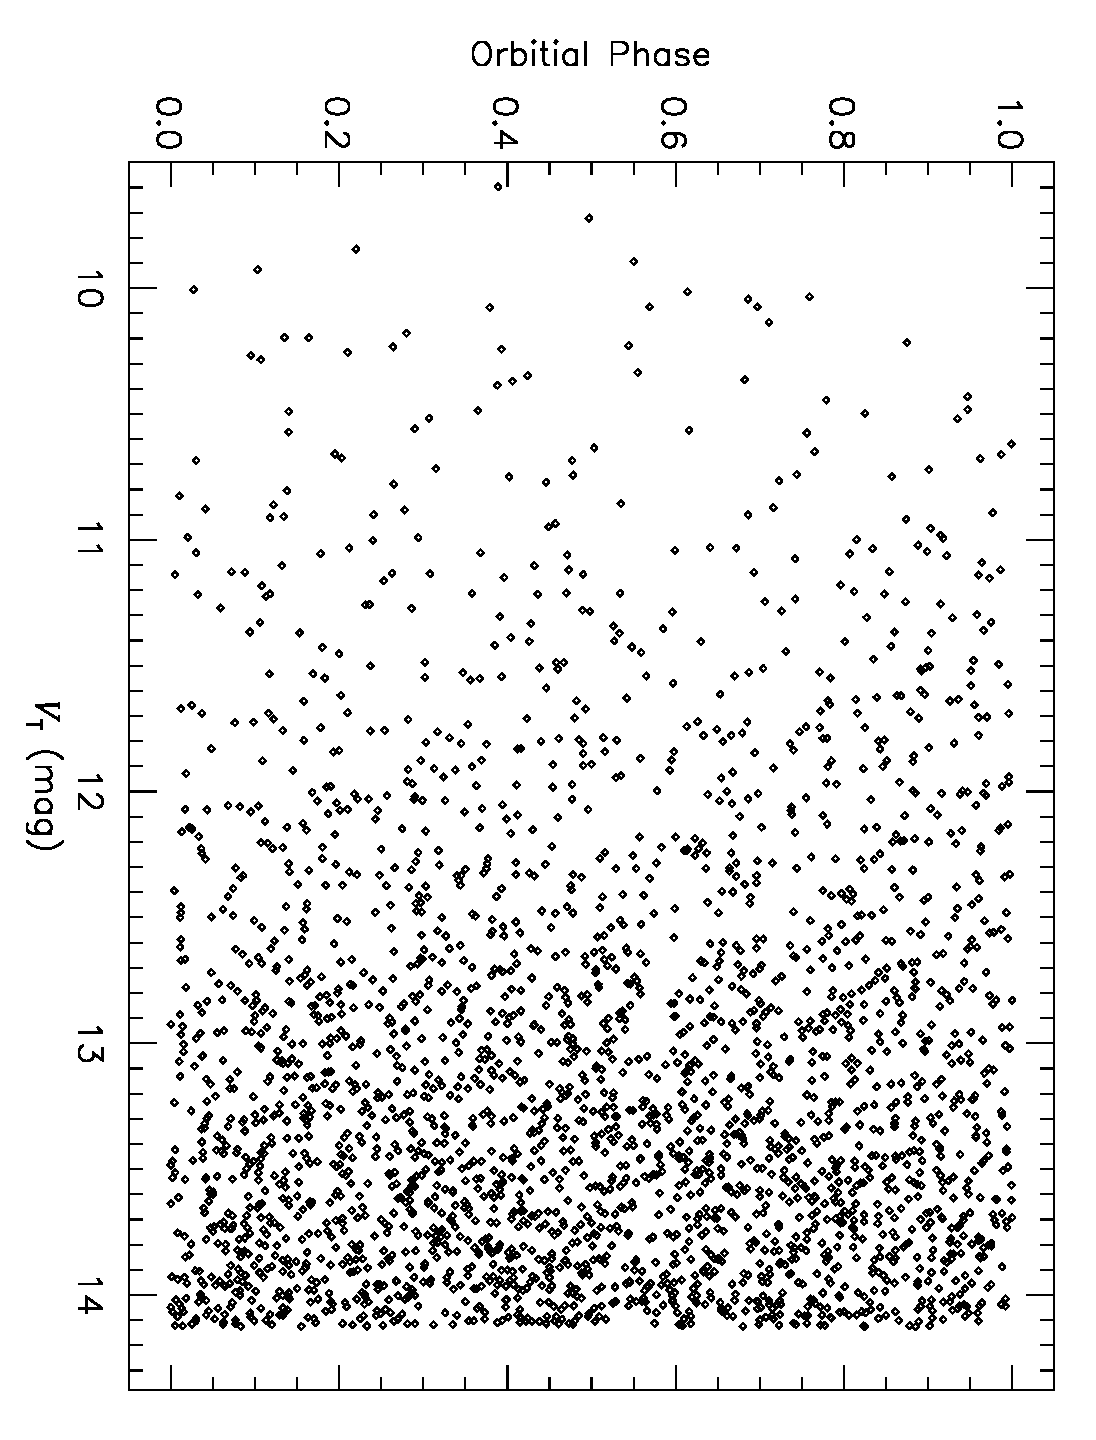
\includegraphics[width=.55\textwidth, angle=90]{7_bls_d}\\
\caption[Randomized values for final two BLS parameters]{%
Same as for figure~\ref{cha:human:sec:model:fig:bls1}, but for %
({\textit top panel}) the fractional transit duration $d$, and %
({\textit bottom panel})  the orbital phase $\Phi$ at the time of transit.
To mimic the output of the BLS algorithm, $d$ and $\Phi$ are kept to 3 decimal places.
The fractional transit duration is only significantly higher than $0.06$ for those candidates with short periods and small stellar radii.
For example, if $d=0.1$, then $a$ must be approximately $3\,R_{\star}$. %
%
}\label{cha:human:sec:model:fig:bls2}
\end{center}
\end{figure}

The BLS transit-search algorithm computes four transit parameters for every input light curve: the orbital period $P$ of the transit, the depth $\Delta$, the fractional duration $d = D/P$ (where $D$ is the duration), and the orbital phase $\Phi$ at the time $T_{c}$ of the transit center.
I generated random values for $P$ ($1\leq P \leq5$\,days; again see figure~\ref{cha:intro:sec:methods:sub:trans:fig:tp}) %
and $\Phi$ ($0\leq \Phi \leq 1$).
Note that while $\Phi$ is normally defined so that $\Phi=0$ at $T_{c}$, here $\Phi$ is defined so that $\Phi=0$ at the start of the TrES observing run.
This is to conform with the definition used by our BLS algorithm for $T_{c}$.
I derived the transit depths from $\Delta = (R_{p}/R_{star})^{2}$, and the fractional transit durations using equation~4 from \citet{Charbonneau_Winn_Latham:apj:2006a}:% chktex 3
\begin{eqnarray*} \label{cha:human:sec:model:eqn:dur}
\sin{i} \cos{\left(\frac{\pi D}{P}\right)} & = & \sqrt{1 - \left(\frac{R_{\star}+R_{p}}{a}\right)^{2}}, \\% chktex 3
 i\sim90\degr \Rightarrow d & = & \frac{1}{\pi} \arccos{\left(\sqrt{1 - \left(\frac{R_{\star}+R_{p}}{a}\right)^{2}}\right)}.% chktex 3
\end{eqnarray*}
Figures~\ref{cha:human:sec:model:fig:bls1} and~\ref{cha:human:sec:model:fig:bls2} shows the distribution of the parameters that should be recovered by the BLS algorithm.
\begin{figure}
\begin{center}
\centering
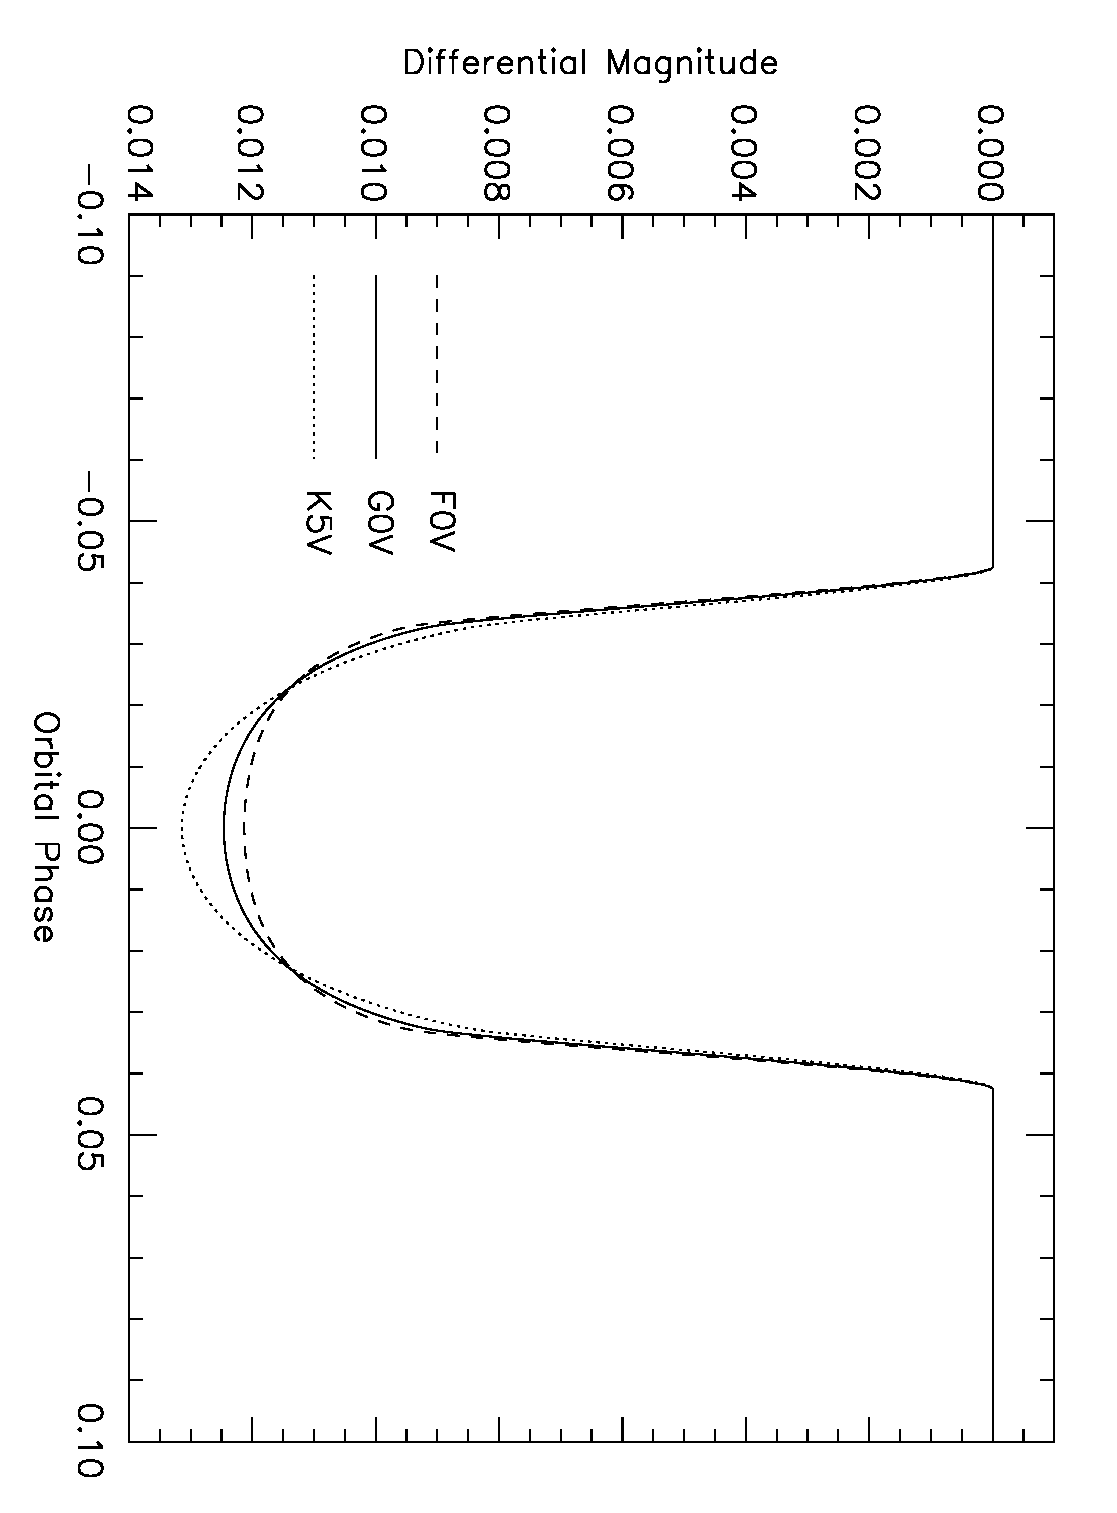
\includegraphics[width=.55\textwidth, angle=90]{7_agol_a}\\
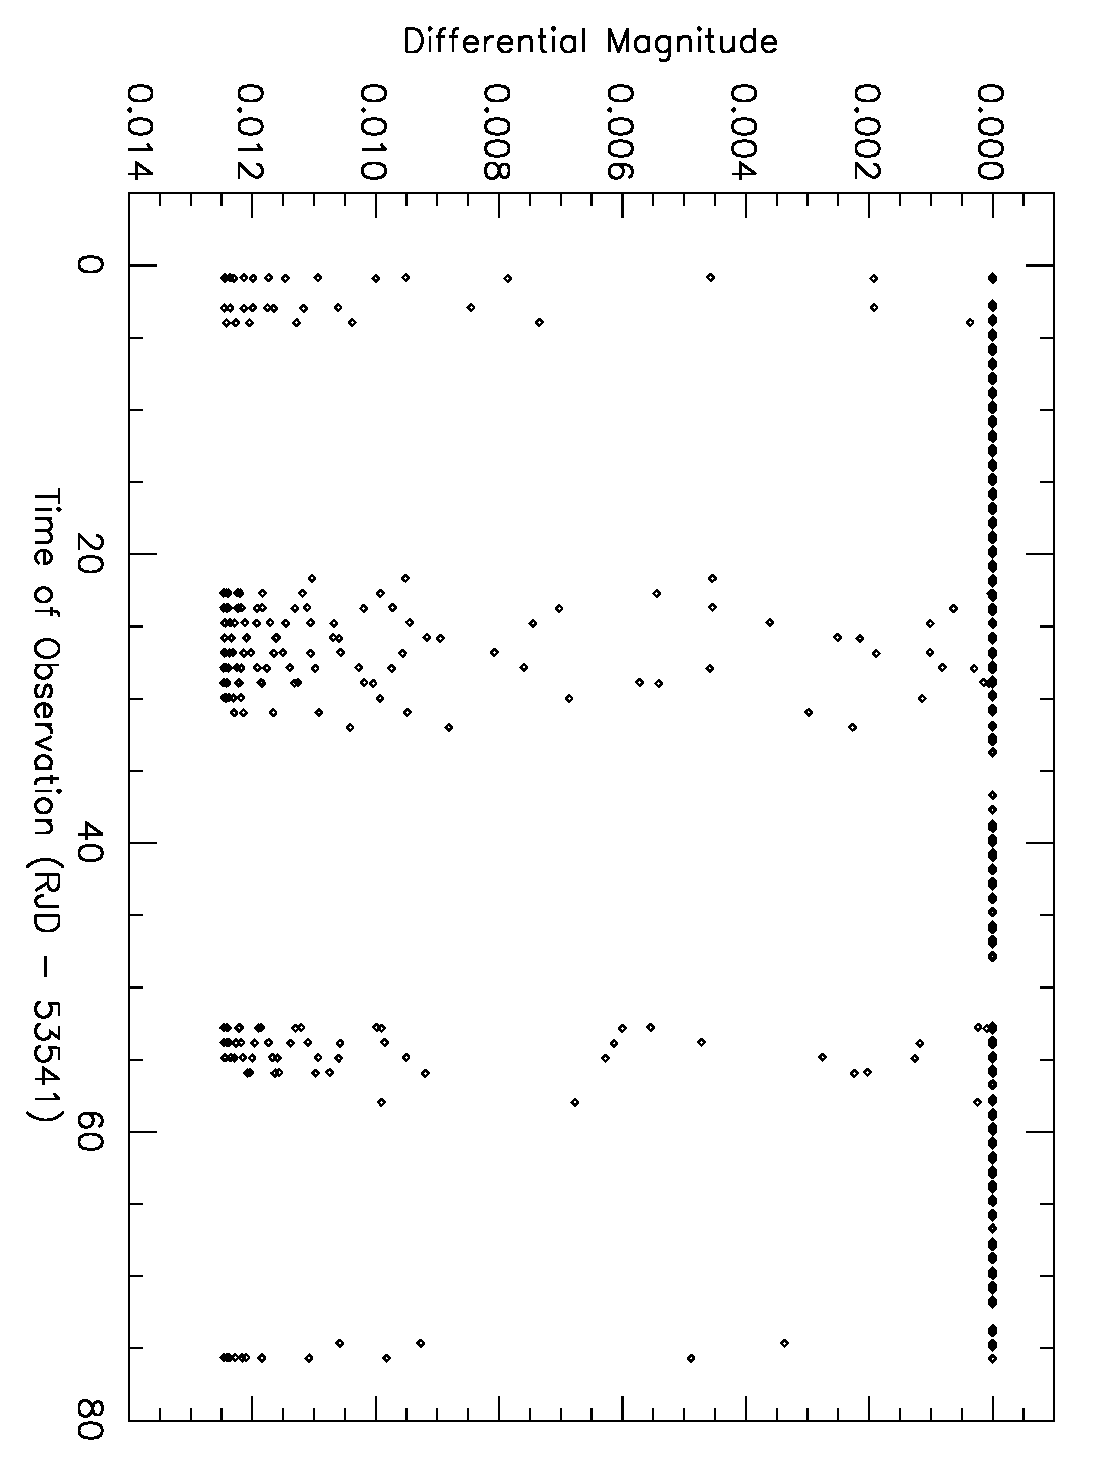
\includegraphics[width=.55\textwidth, angle=90]{7_agol_b}\\
\caption[Example of model transits]{%
({\textit Top}) %
Model transit light curves for a 1.2\% transit with a period of 1.038588\,days.
The shape of the three light curves is determined by the limb-darkening associated with the specified spectral type.
Distinguishing between these light curves is not possible for the TrES photometry, hence I simply assumed the G0V limb-darkening coefficients.
({\textit Bottom}) Model transit light curve from the {\textit top panel} plotted versus the times of observation during the TrES Lyr-1 run. %
}\label{cha:human:sec:model:fig:agol}%
\end{center}
\end{figure}

\begin{figure}
\begin{center}
\centering
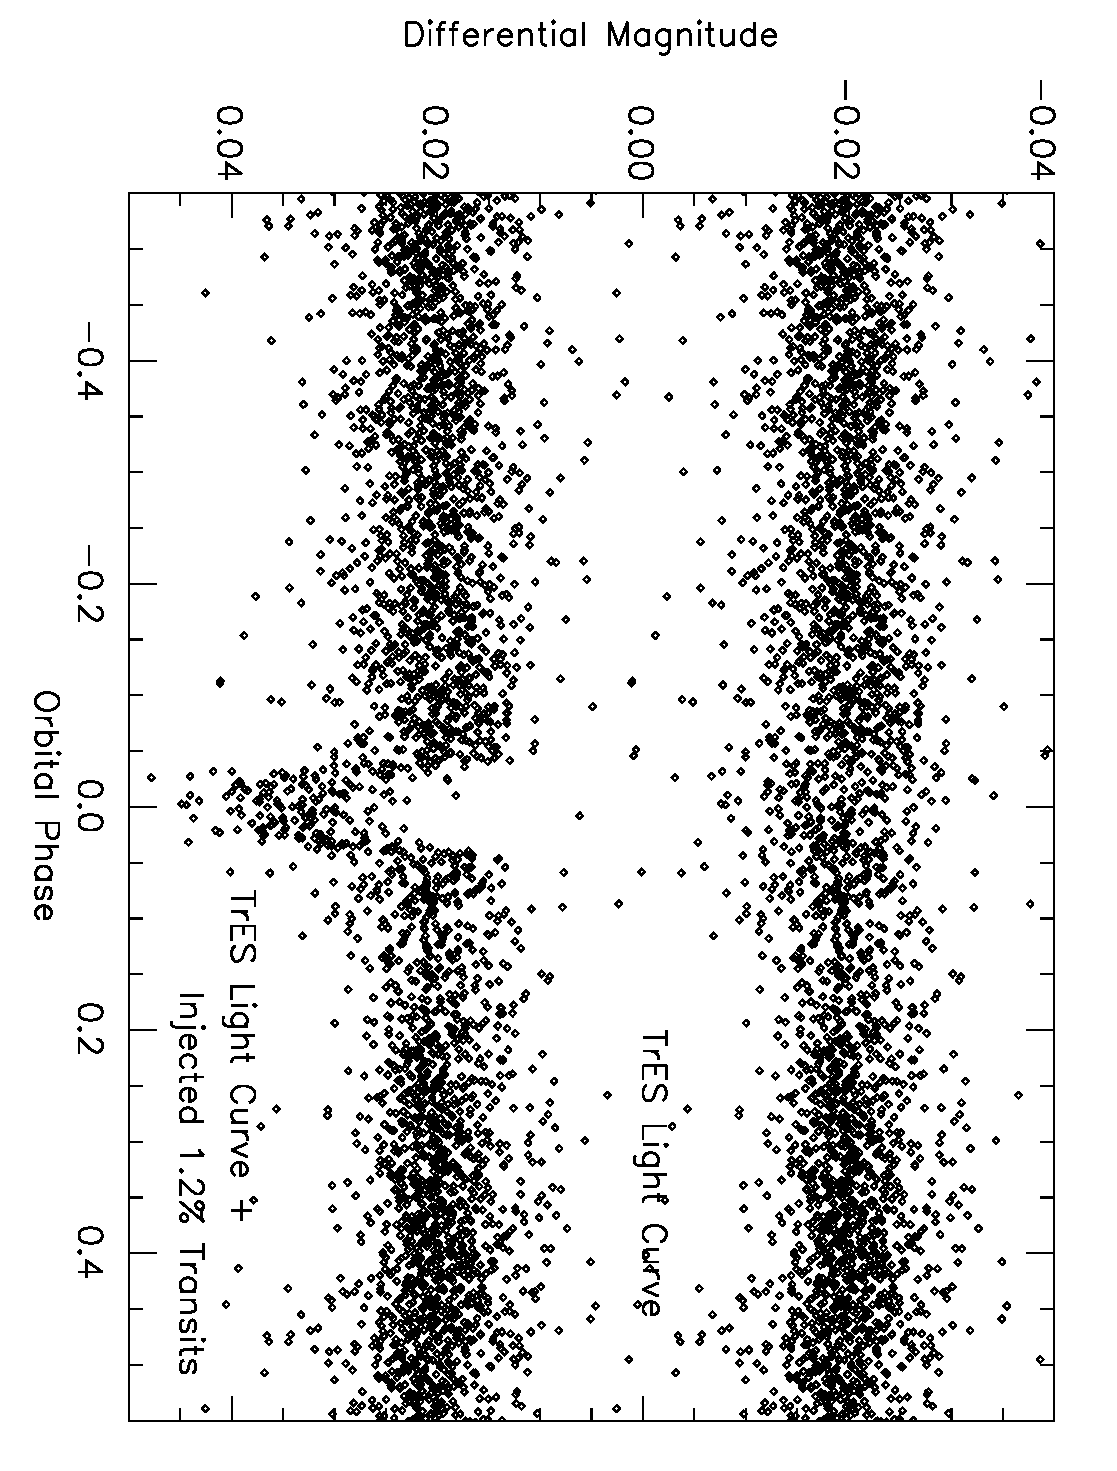
\includegraphics[width=.75\textwidth, angle=90]{7_agol_c}\\
\caption[Example of TrES light curve with injected transits]{%
The {\textit top} light curve is from the TrES Lyr1 field, phased to an orbital period of 1.038588\,days. The {\textit bottom} light curve shows the results of injecting the model transits from figure~\ref{cha:human:sec:model:fig:agol}%
.%
}\label{cha:human:sec:model:fig:inject}%
\end{center}
\end{figure}

Using these random system parameters as unseen input, I generated model transit light curves using code based on the analytic formulae of \citet{Mandel_Agol:apjl:2002a}.
This code computes the variation with time in the amount of obscuration of a limb-darkened source by a dark body, by deriving the area of the source obscured at that time, and outputs this variation in terms of relative flux.
Although the TrES photometry is too noisy to discern between different limb-darkening due to different stellar spectral types, the code requires limb-darkening coefficients as part of the input.
I assumed a quadratic limb-darkening model of the form:
\begin{eqnarray*}\label{cha:human:sec:model:eqn:limb}
I(\mu)/I(1) = 1-a(1-\mu)-b(1-\mu)^2,% chktex 3
\end{eqnarray*}
where $\mu=\cos{\gamma}$, $\gamma$ is the angle between the line of sight and the local normal to the stellar surface, $I$ is the specific intensity, and $a$ and $b$ are the limb-darkening coefficients.
The $R$-band quadratic limb-darkening coefficients for a G0V star (a typical spectral type from my data; see figure~\ref{cha:human:sec:model:fig:jmks}) are $a=0.2938$ and $b=0.3441$ ($T_{\mathrm eff}=6000$\,K, $\log{g}=4$, [Fe/H]=0, $V_{\mathrm turb}=0\,\kms$; \citealt{Claret:aa:2000a}).
figure~\ref{cha:human:sec:model:fig:agol} %
shows a phased model light curve using these coefficients and assuming $R_{p}/R_{\star}=0.1$.
figure~\ref{cha:human:sec:model:fig:agol} %
also shows model light curves displaying limb-darkening associated with a K5V and F0V star.
Distinguishing between the different limb-darkening requires photometry with exquisite precision (such as seen in \citealt{Brown_Charbonneau_Gilliland:apj:2001a}).
I simply assumed a G0V spectral type and luminosity class for my analysis.

I then accounted for the actual temporal coverage of the observations.
The effect of this can be seen in the {\textit bottom panel} of figure~\ref{cha:human:sec:model:fig:agol}%
, where the model from the {\textit top panel} have been plotted versus the times of observation of the Lyr1 field.
The final product of the TrES pipeline is a series of light curves, one for each star in the field.
These light curves have been decorrelated to remove systematics suffered by wide-field transit surveys, and averaged (in 9-minute bins) to reduce the computational effort of the BLS transit search.
For this test, I chose the combined binned TrES data set, with observations from both Sleuth%
\footnote{See \url{http://www.astro.caltech.edu/\~ftod/tres/}.}%
\ (Palomar Observatory, California; \citealt{ODonovan_Charbonneau_Kotredes:AIP:2004a}) and the Planet Search Survey Telescope (PSST;\@Lowell Observatory, Arizona; \citealt{Dunham_Mandushev_Taylor:pasp:2004a}).
Since these TrES time series and model light curves both have units of magnitudes, I added to the time series for each fake host star the corresponding model light curve to produce the fake time series.
The light curves of the stars not chosen as fake hosts were untouched.
Figures~\ref{cha:human:sec:model:fig:inject} shows the result of injecting the model light curve from figure~\ref{cha:human:sec:model:fig:agol} %
into a real time series from the Lyr1 field.

\section{BLS and Visual-Recovery Methods of Injected Transits}\label{cha:human:sec:rec}

\begin{figure}
\begin{center}
\centering
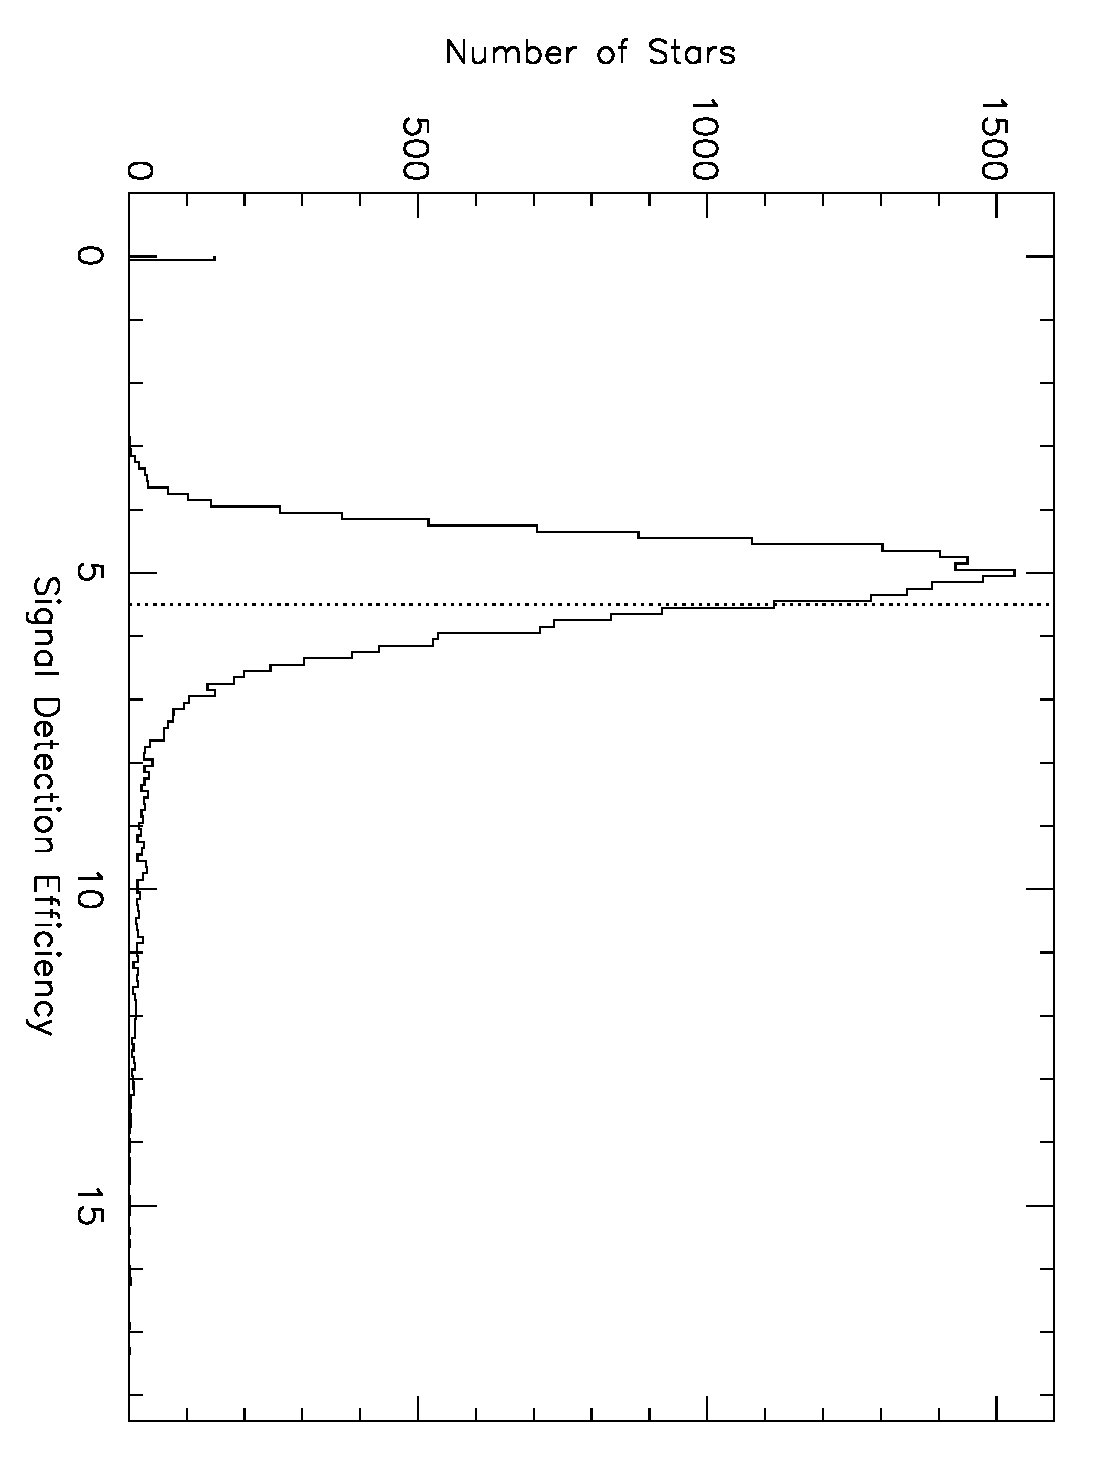
\includegraphics[width=.55\textwidth, angle=90]{7_sde_a}\\
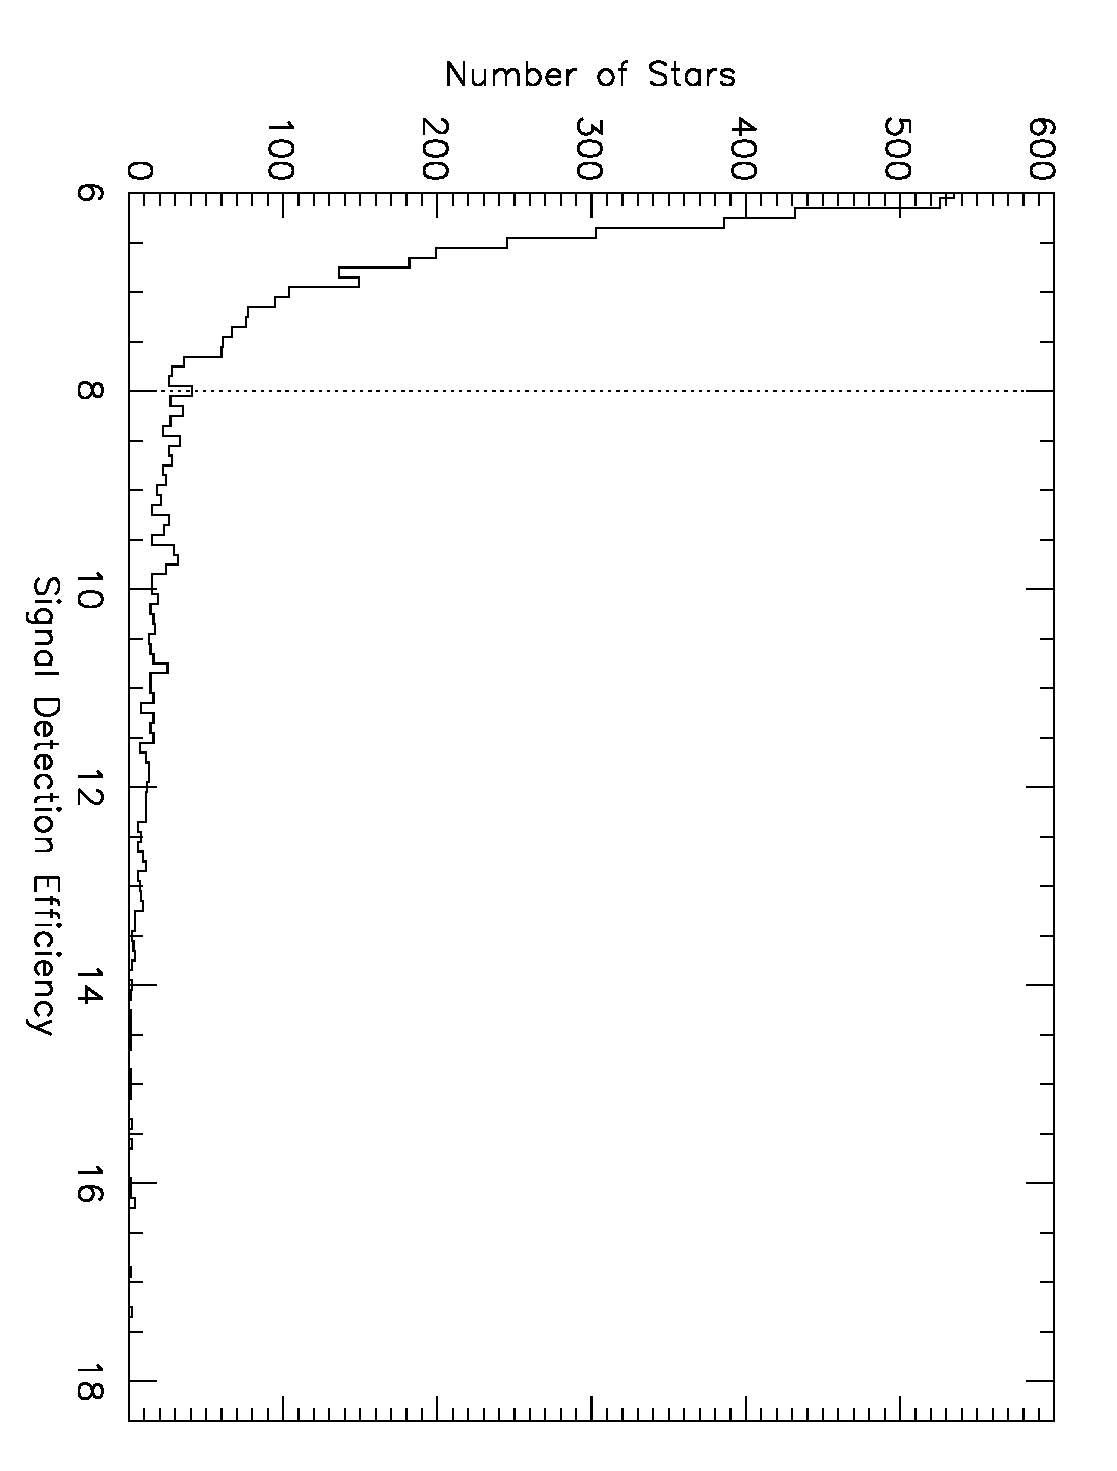
\includegraphics[width=.55\textwidth, angle=90]{7_sde_b}\\
\caption[Histograms of BLS SDEs for fake data set]{%
Histograms of the Signal Detection Efficiency (SDE) derived by the Box-fitting Least-Squares transit-search algorithm for: %
({\textit top panel}) the entire TrES Lyr1 data set with injected transits, and %
({\textit bottom panel}) those candidates with $\mathrm{SDE}\geq6$.
Saturated stars or stars with very noisy data were skipped by the algorithm, and assigned an SDE of 0.
The {\textit dotted} line in the {\textit top panel} denotes the minimum SDE of a candidate that will be visually inspected.
I first examined the candidates with SDEs to the right of the {\textit dotted} line in the {\textit bottom panel}, as they are more likely not to be spurious detections caused by random noise.
}\label{cha:human:sec:model:fig:sde}
\end{center}
\end{figure}


\begin{figure}
\begin{center}
\centering
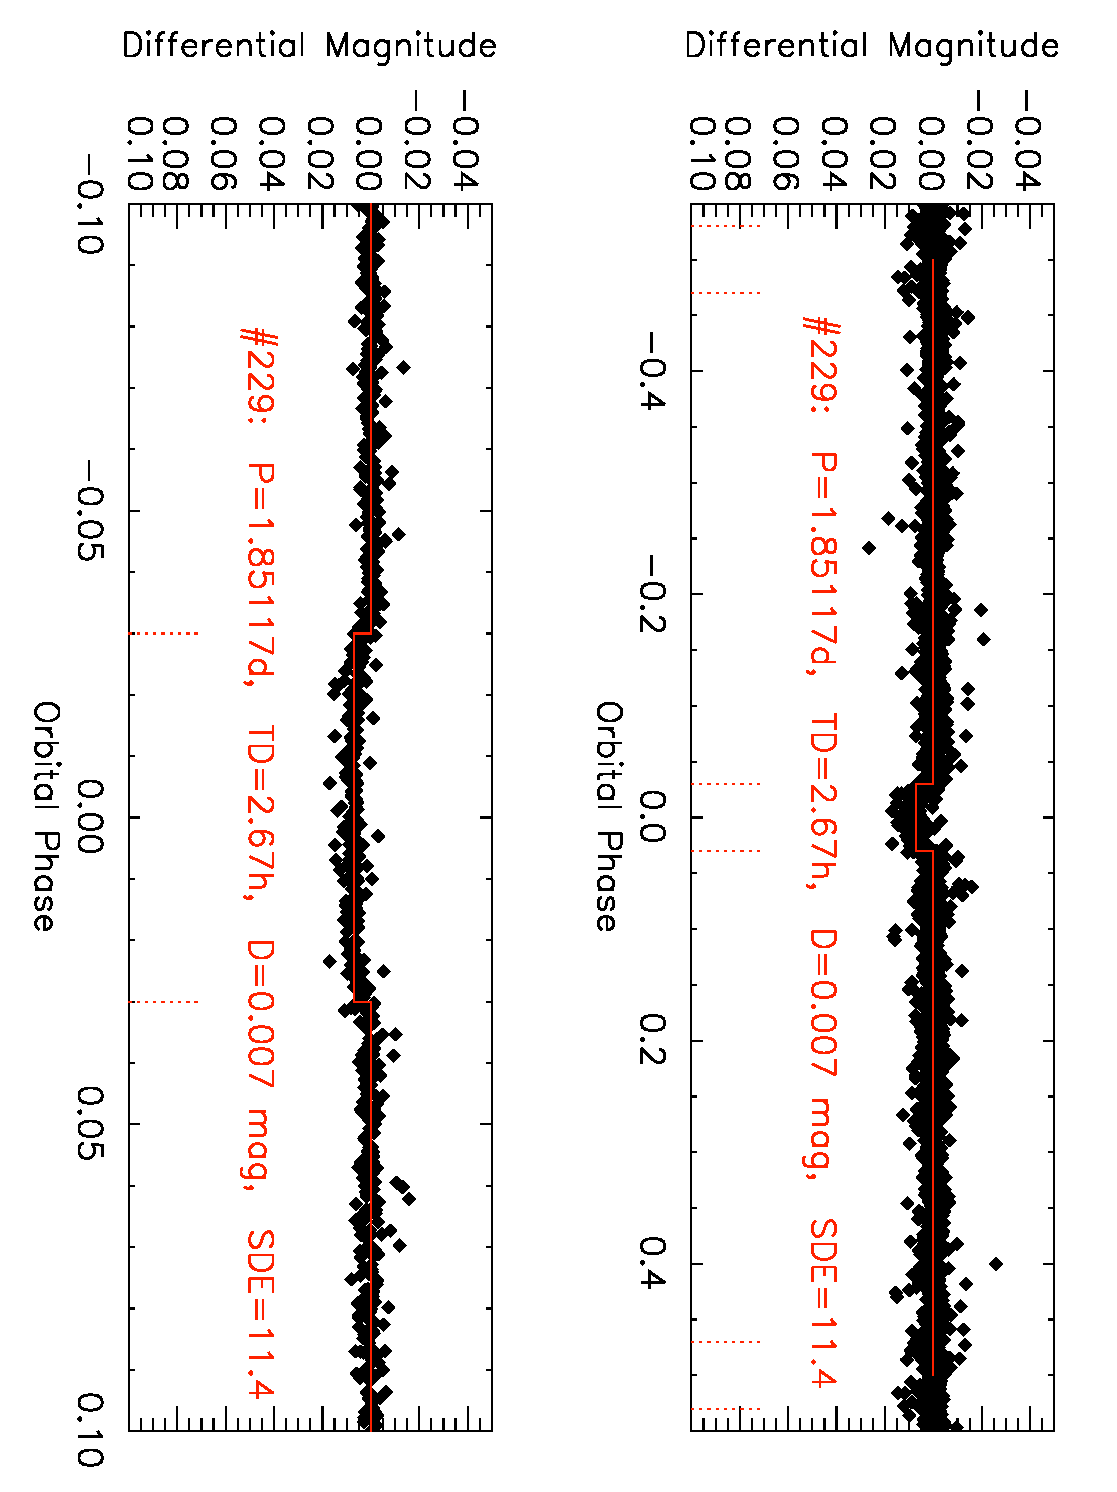
\includegraphics[width=.75\textwidth, angle=90]{7_highsde}
\caption[Example of an injected transit candidate with a high SDE]{%
Example of an injected transit candidate detected by the Box-fitting Least-Squares (BLS) algorithm with a high ($\geq$8) Signal Detection Efficiency (SDE).
Both plots show the variation in differential magnitude with orbital phase, and the four parameters (period P, duration TD, depth D, and SDE) output by the BLS algorithm are superimposed.
The {\textit upper} plot shows the entire orbit, whereas the {\textit lower} plot is at near-transit.
The {\textit dotted red lines} in both plots indicate (i) the point of ingress and egress of the box-transit (taken as $\pm d$, where $d$ is the BLS fractional duration), and (ii) this region shifted by 0.5 in phase to highlight the location where a secondary eclipse might be spotted.
I view plots similar to these for each transit candidate to determine the detection is real or spurious.%
}\label{cha:human:sec:model:fig:highsde}
\end{center}
\end{figure}

Treating the fake time series as a real data set from a TrES field, I then continued with the TrES procedure for identifying candidate transiting planets.
I searched the time series for periodic transit-like dips using the BLS algorithm, which assigns a Signal Detection Efficiency (SDE, see appendix~\ref{cha:bls}) statistic to each star based on the strength of the transit detection.
It represents a signal-to-noise ratio, where the signal is the average differential magnitude inside the transit compared to the average differential magnitude outside the transit, and the noise is the scatter of the differential magnitudes inside the transit.
I restricted my search to the period range (0.5--5\,days) and fractional duration range ($\sim$0.01--0.1) that I normally use for TrES data.
I restrict myself to periods less than 5\,days due to the necessity for a transit detection of observing multiple transits during an observing run, which typically lasts for TrES for about 40 clear nights.
The fractional duration range is based on what we would expect (\citealp*{Defay_Deleuil_Barge:aa:2001a}, and see figure~\ref{cha:human:sec:model:fig:bls2}) over a wide range of physical parameters, such as those chosen for this analysis, and for these orbital periods. Figure~\ref{cha:human:sec:model:fig:sde} shows a histogram of the derived SDEs for this fake data set.
From this figure, I chose $\mathrm{SDE}=8.0$ as a lower limit for my first visual examination, that of the candidates with the most significant detections.
Since there are few candidates with $\mathrm{SDE}\geq8.0$, I could concentrate on the best candidates without being overwhelmed by spurious transit light curves.
I then examined the candidates with $5.5 \leq \mathrm{SDE} < 8.0$ to find any remaining interesting candidates.
The lower limit here is taken to be just below the $\mathrm{SDE}=6$ limit that minimizes statistical false positives seen in \citet{Kovacs_Zucker_Mazeh:aa:2002a}.
Beyond this point, it will be difficult to find any true transit candidate, as the transit signal will be low and there will be many spurious transit light curves with similar SDEs.
Starting with the brightest stars, I examined each of the light curves with SDE$\geq8$, and then the light curves with $5.5<\mathrm{SDE}<8$.
I limited my search to candidates with $0.02 \leq (P\ \mod\ 0.5\,\mathrm{days})\leq 0.48$ and 0.004\,mmag $\leq \Delta \leq 0.1$\,mmag.
This limit avoids spurious detections with both integer or half-integer periods that are caused by a few bad data points within the supposed transit. Figure~\ref{cha:human:sec:model:fig:highsde} is an example of a plot of a high SDE candidate that I examined.

\section{BLS and Visual-Recovery Rates}\label{cha:human:sec:recrates}

The visual recovery of a transit light curve is heavily dependent on the accuracy of BLS transit parameters used to produce a phased light curve for inspection.
Therefore, as a first step in determining my ability to recover the fake transit light curve, I examined the recovery rate of injected transits for the BLS transit search.
The four parameters computed by BLS for each input light curve are the orbital period $P$ of the transits, the depth $\Delta$, the fractional duration $d$, and the orbital phase $\Phi$.
Of these, the most important is $P$.
As long as the light curve is correctly phased, I should be able to visually identify the transit.
Although the parameters $\Delta$, $d$, and $\Phi$ are used to overlay a model box-transit light curve and aid visual recovery, transit recovery is still possible if these parameters are highly inaccurate.
From experiments with several light curves where I varied the period used to phase the light curve while maintaining a visible transit signal, I chose the first recovery criterion to be that the derived orbital period is within 0.1\% of the true value.
The second criterion is that the derived transit ``depth'' is not negative.
This is because a transit light curve with a negative ``depth'' is automatically skipped by the code used to plot the transit candidates.

\begin{figure}
\begin{center}
\centering
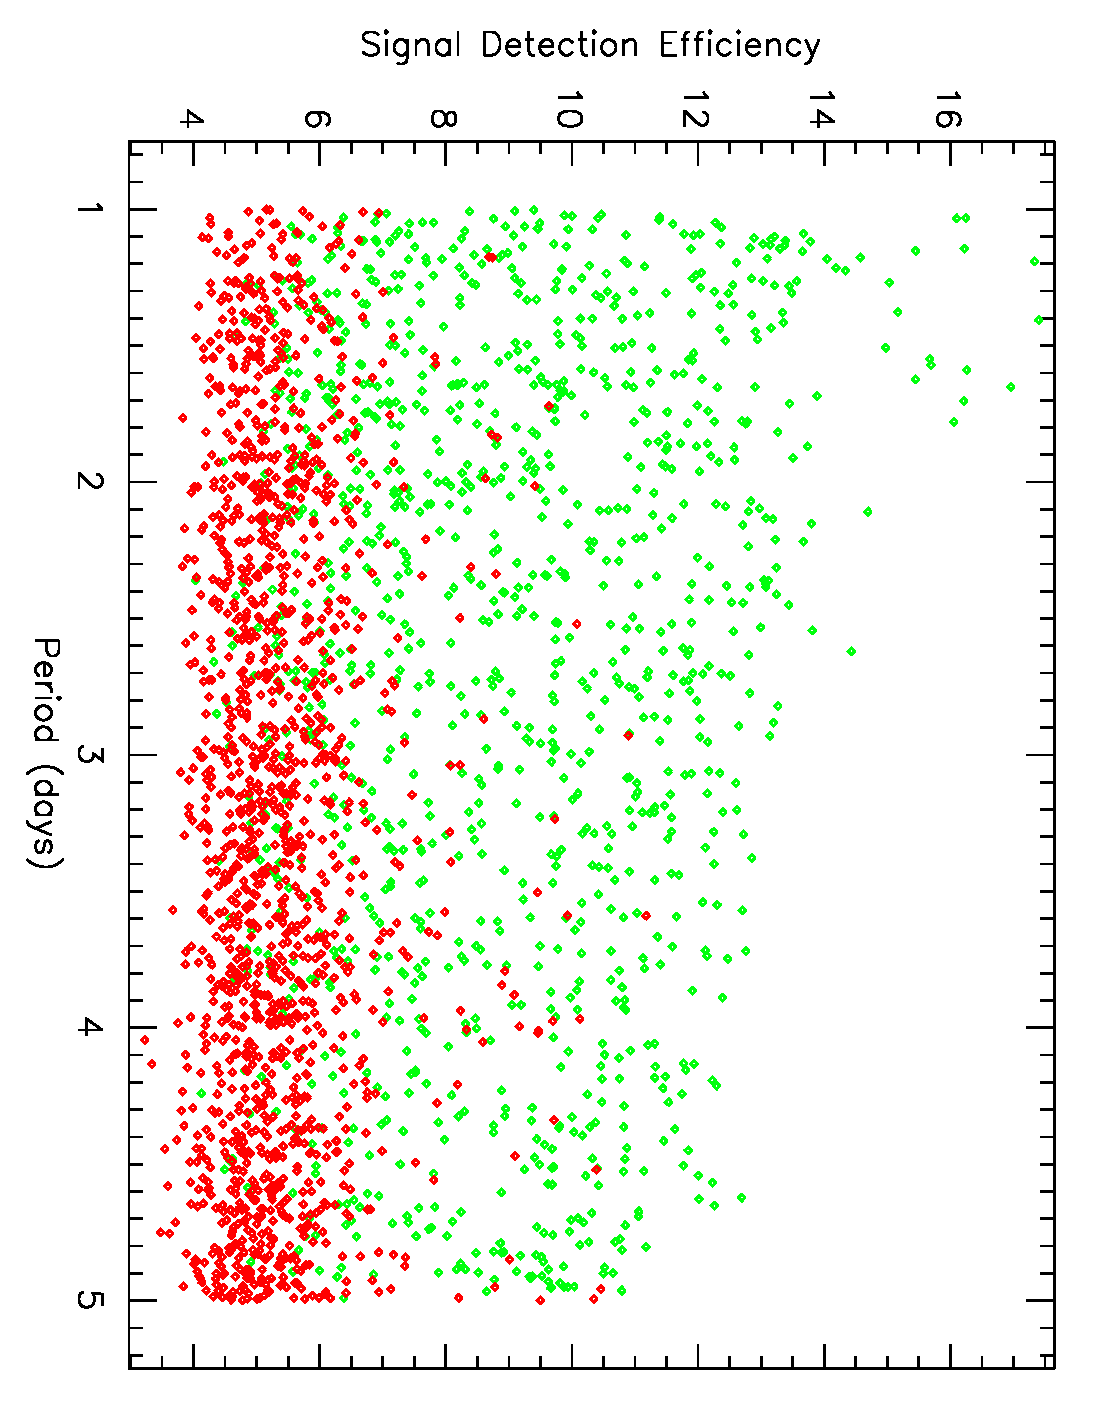
\includegraphics[width=.55\textwidth, angle=90]{7_comp_b} \\
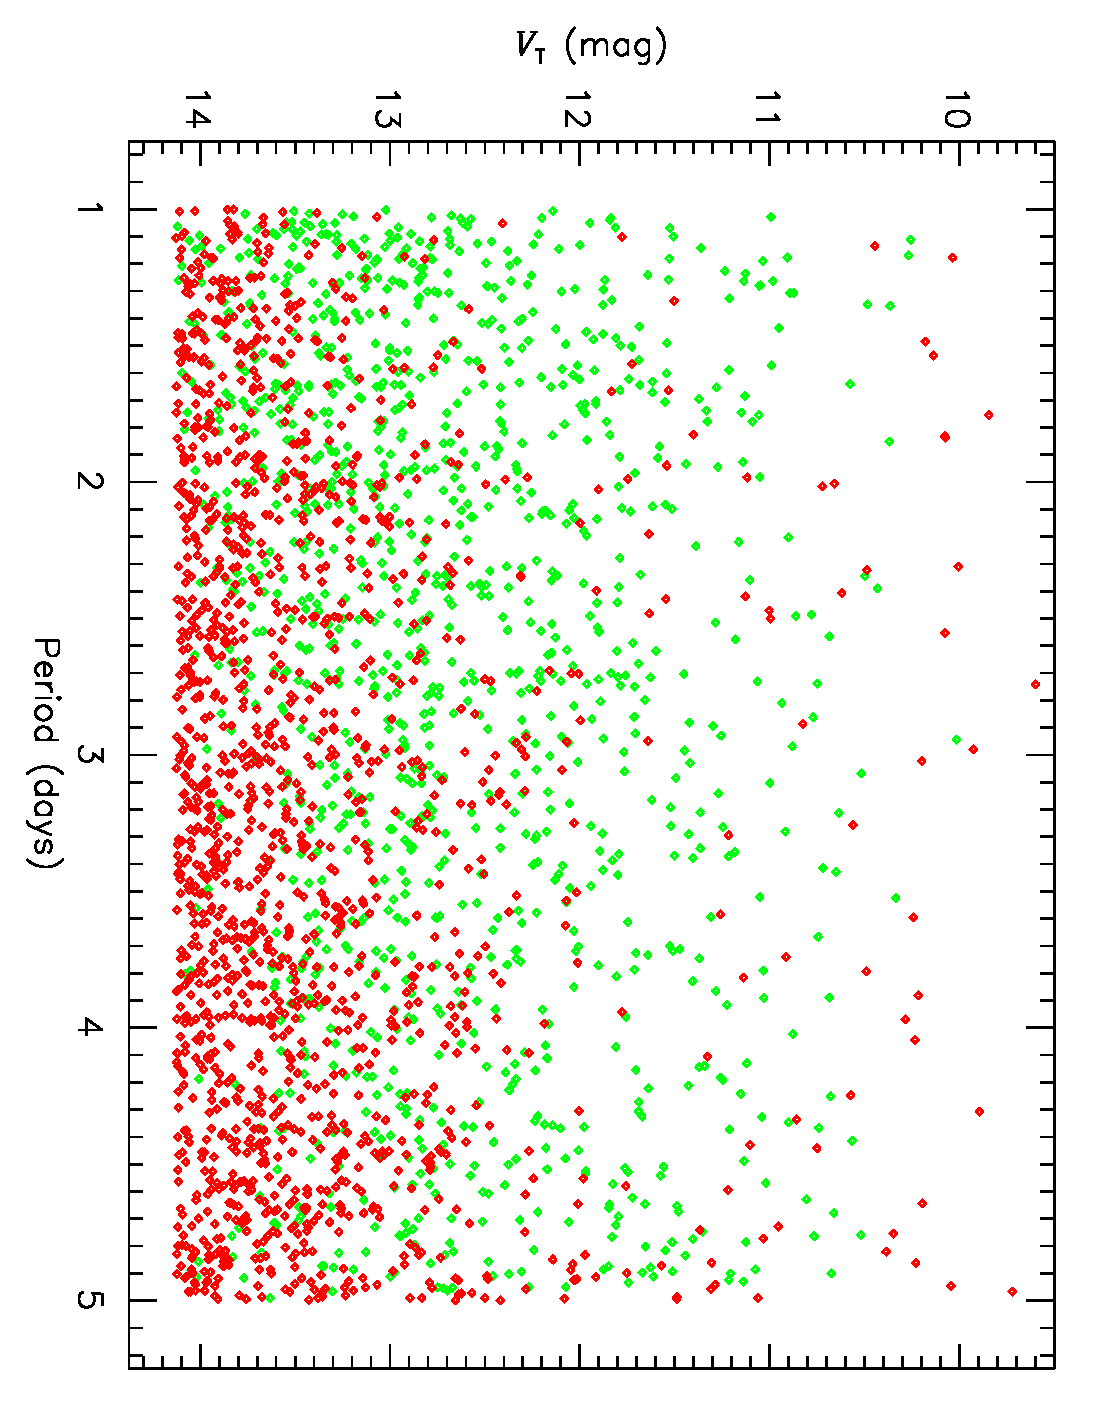
\includegraphics[width=.55\textwidth, angle=90]{7_comp_a} \\
\caption[SDE and $V_{T}$ versus period for BLS-recovered transits]{%
({\textit Top}) Signal Detection Efficiencies (SDEs) of the injected transit candidates plotted against their orbital period.
The candidates marked in {\textit green} were recovered by the Box-fitting Least-Squares (BLS) algorithm; that is, the derived orbital period was accurate to within 0.1\% and the transit depth was not negative.
{\textit Red diamonds} signify candidates not recovered by BLS.\@
BLS recovered the majority (79\%) of injected transit candidates with $\mathrm{SDE}\gsim6$.
({\textit Bottom}) Approximate $V_{T}$ magnitudes versus orbital period for the injected transit candidates.
BLS recovered 62\% of candidates with $V\leq13.5$\,mag.%
}\label{cha:human:sec:model:fig:rec}
\end{center}
\end{figure}

\begin{figure}
\begin{center}
\centering
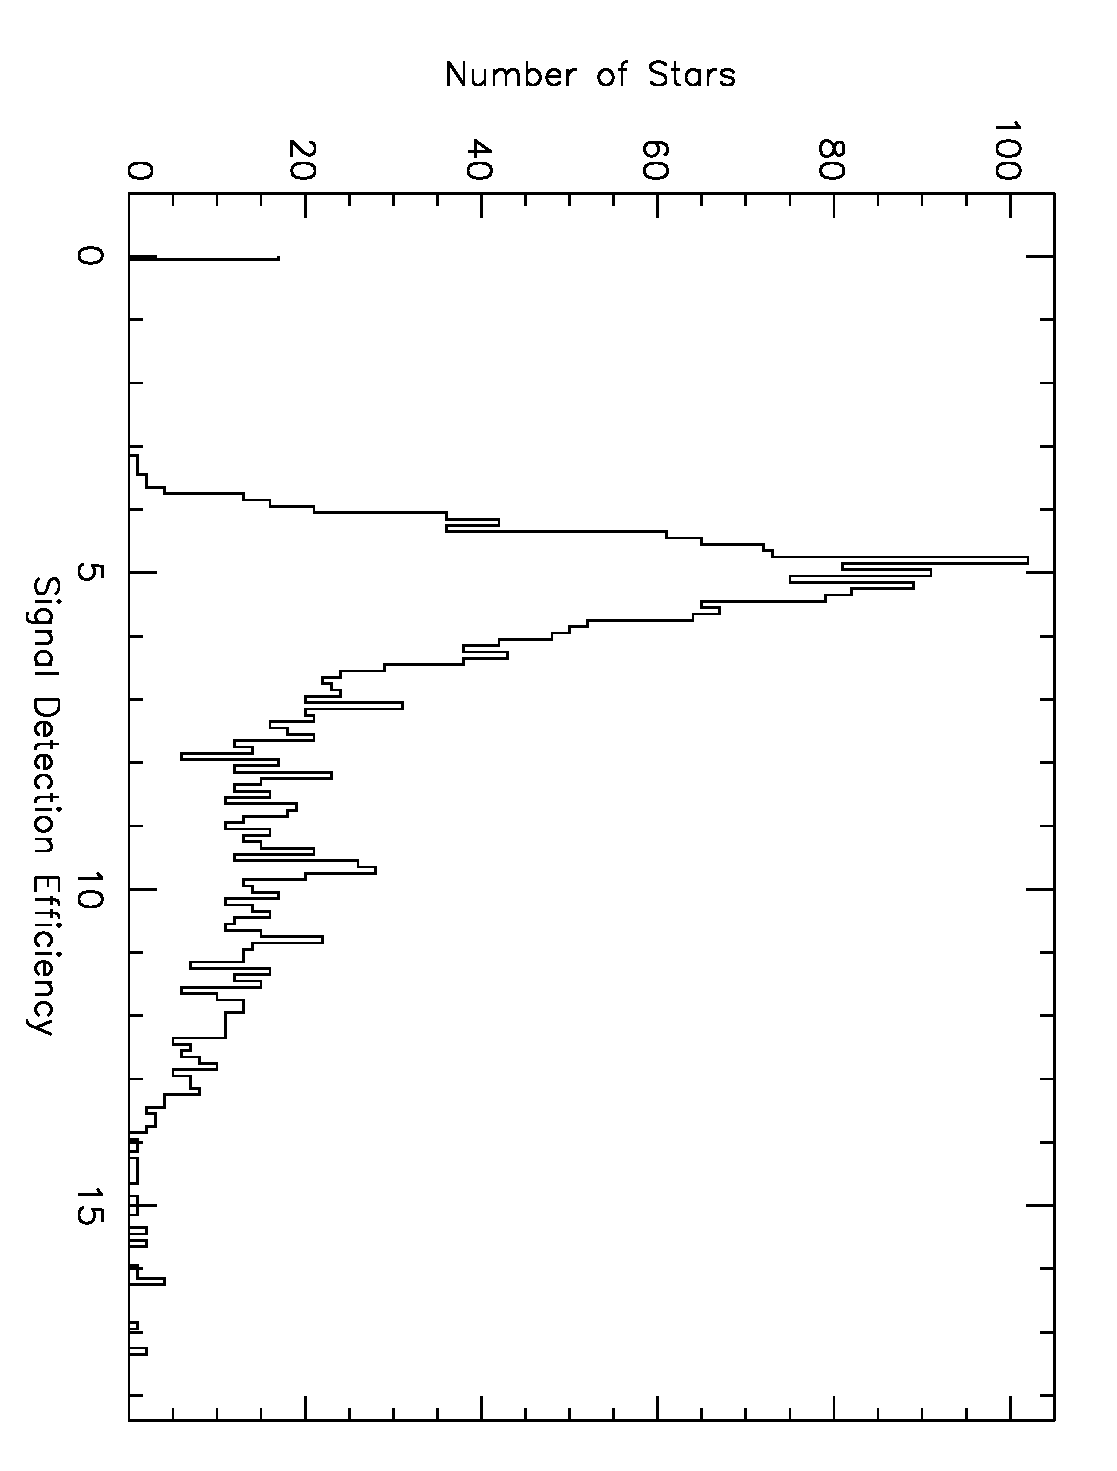
\includegraphics[width=.75\textwidth, angle=90]{7_comp_f}
\caption[Histogram of SDEs for BLS-recovered transit candidates]{%
Histogram of the Signal Detection Efficiency (SDE) derived by the Box-fitting Least-Squares transit-search algorithm for the injected transit candidates.%
}\label{cha:human:sec:model:fig:histsderec}
\end{center}
\end{figure}
\begin{figure}
\begin{center}
\centering
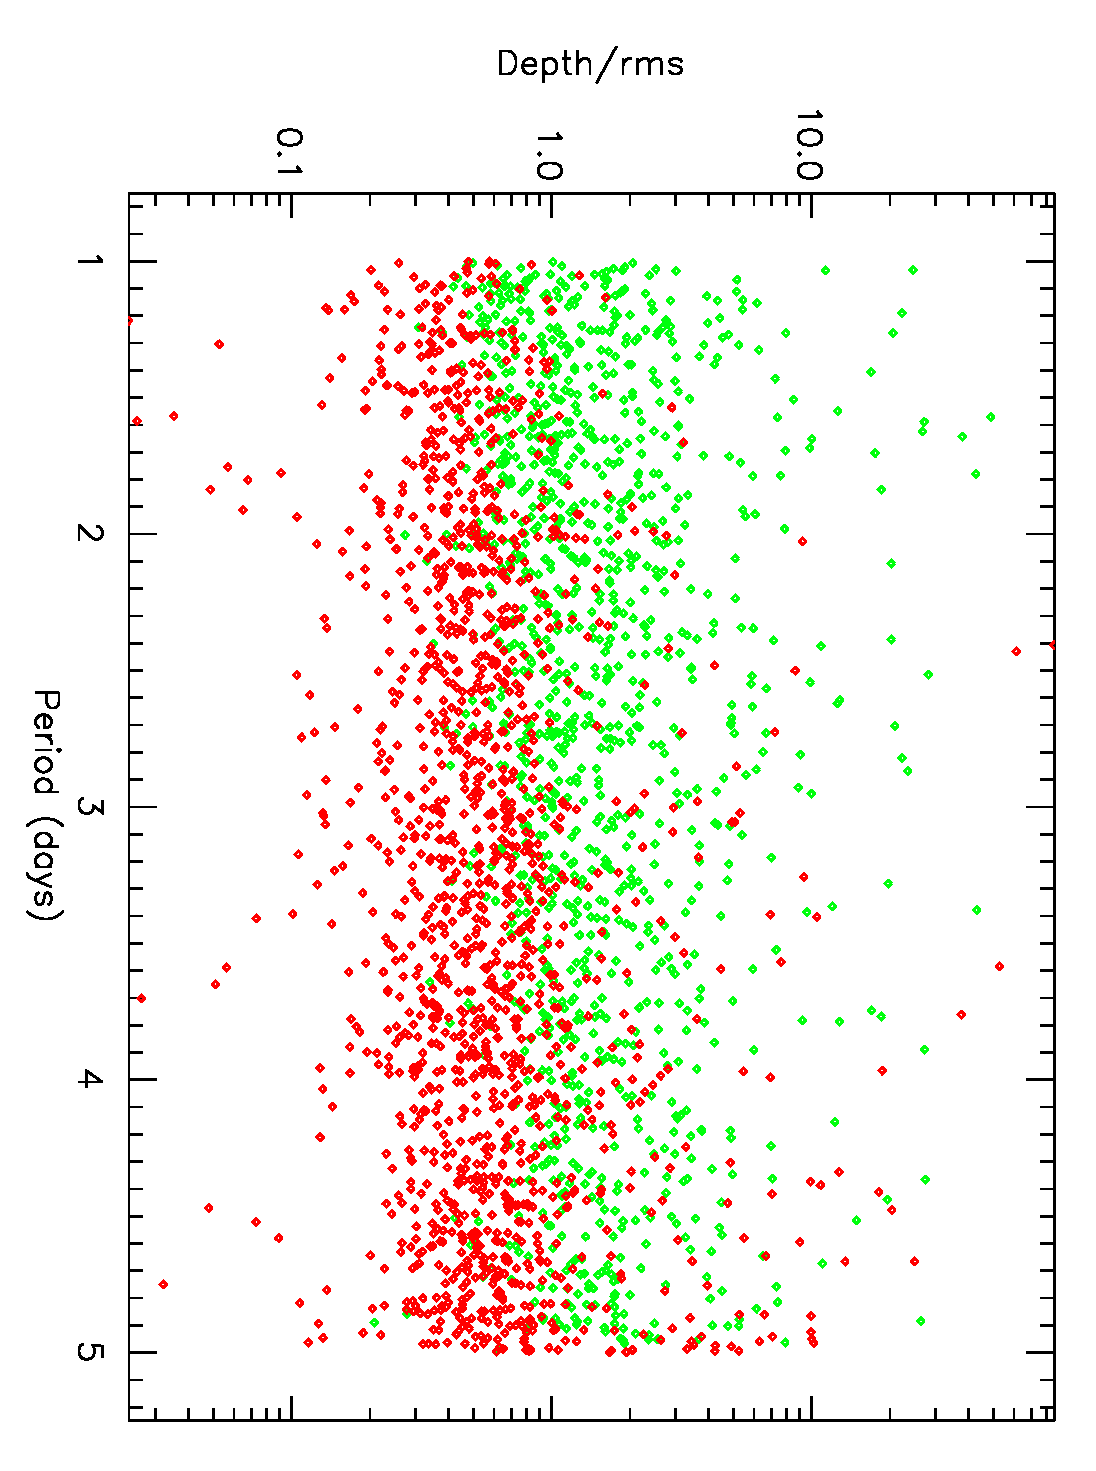
\includegraphics[width=.75\textwidth, angle=90]{7_comp_c} \\
\caption[Ratio of $\Delta$ to $\sigma$ versus period for BLS-recovered transits]{%
Same as figure~\ref{cha:human:sec:model:fig:rec}, but for the ratio of the transit depth ($\Delta$) to the rms ($\sigma$) of the TrES photometry.
Of the candidates with $\Delta\gsim\sigma$, 77\% were recovered by the transit-search algorithm (marked in {\textit green}; the candidates not recovered are in {\textit red}).%
}\label{cha:human:sec:model:fig:ratiorec}
\end{center}
\end{figure}

Of the 2,612 injected transit candidates, 1,153 were recovered by the BLS transit-search algorithm.
figure~\ref{cha:human:sec:model:fig:rec} %
shows the SDEs of these fake candidates, where the candidates in {\textit green} were recovered by the BLS algorithm and those in {\textit red} were not.
(A histogram of these SDEs for comparison with figure~\ref{cha:human:sec:model:fig:sde} can be seen in figure~\ref{cha:human:sec:model:fig:histsderec}.)
As can be clearly seen, the transit-search algorithm recovered the majority (79\%) of candidates with $\mathrm{SDE} \gsim 6$ but few with $\mathrm{SDE} < 6$. The latter are not significant detections \citep[see][]{Kovacs_Zucker_Mazeh:aa:2002a}.
The BLS recovery of candidates in terms of the magnitudes of the host star can also be seen in figure~\ref{cha:human:sec:model:fig:rec}%
.
Here the TrES instrumental $r$-band magnitude has been converted to an approximate Tycho-2 \citep{Hog_Fabricius_Makarov:aa:2000a} $V_{T}$ magnitude using the field stars with known $V_{T}$.
Again, the BLS algorithm recovers the majority (62\%) of transit candidates with $V_{T}\lsim 13.5$\,mag, except for the brighter, saturated stars.
These results can be better understood by comparing the transit depth to the rms ($\sigma$) of the photometry for the host star, as shown in figure~\ref{cha:human:sec:model:fig:ratiorec}. Of the transit candidates with $\Delta \gsim \sigma$,  77\% are recovered, with a slight bias against longer periods.

This suggests that $V_{T}\lsim 13.5$\,mag and $\Delta \gsim \sigma$ are the limits for the BLS algorithm as applied to TrES data.
Of the 1,459 candidates not recovered by the BLS algorithm, 1,197 had $\mathrm{SDE} < 6$, 868 had $V_{T}> 13.5$\,mag, and 1,230 had $\Delta < \sigma$. When these factors are taken into account, only 39 (1\%) candidate transit signals that we would expected the algorithm to detect were not recovered.

\begin{figure}
\begin{center}
\centering
\includegraphics[width=.55\textwidth, angle=90]{7_comp_d}\\
\includegraphics[width=.55\textwidth, angle=90]{7_comp_e}\\
\caption[BLS recovery rates for different orbital periods and planetary radii]{%
Percentage of the injected transit candidates recovered by the automated BLS transit-search algorithm as a function of approximate $V_{T}$ magnitude for different ranges in: %
%($a$)
({\textit top panel}) orbital period $P$, and %
%($b$)
({\textit bottom panel}) planetary radii $R_{p}$. %
The recovery rates have been averaged in bins in $V_{T}$ of 0.5\,mag.%
}\label{cha:human:sec:model:fig:recrates1}
\end{center}
\end{figure}

\begin{figure}
\begin{center}
\centering
\includegraphics[width=.55\textwidth, angle=90]{7_comp_h}\\
\includegraphics[width=.55\textwidth, angle=90]{7_comp_i}\\
\caption[BLS recovery rates for different stellar radii and impact parameters]{%
Same as for figure~\ref{cha:human:sec:model:fig:recrates1}, but for: %
%($a$)
({\textit top panel})  stellar radii $R_{\star}$, and %
%($b$)
({\textit bottom panel})  impact parameters $b$. %
}\label{cha:human:sec:model:fig:recrates2}
\end{center}
\end{figure}

The variation of the recovery rate with stellar magnitude for different orbital periods, planetary radii, stellar radii and impact parameters is shown in figures~\ref{cha:human:sec:model:fig:recrates1} and~\ref{cha:human:sec:model:fig:recrates2}.
As would be expected, the recovery rates drop for the fainter stars ($V_{T}>$13.5 mag) and the brightest, saturated stars ($V_{T}<$10.0\,mag).
The rate also increases for shorter periods, larger planets, and smaller stars, although the trend is not robust due to the relatively small number of candidate transits.
This bias is not surprising, as a larger planet and smaller star increases $\Delta$, and a shorter period increases the number of observed transits. However, the rate does seem to increase slightly with larger impact parameters, which is surprising. A large impact parameter implies a V-shaped light curve indicative of an eclipsing binary, rather than the typical transit light curve.
Overall, the recovery rate for the BLS algorithm is about 80\% for the average magnitudes of $11 \leq V_{T} \leq 12$\,mag.

\begin{figure}
\begin{center}
\centering
\includegraphics[width=.55\textwidth, angle=90]{7_visual_b} \\
\includegraphics[width=.55\textwidth, angle=90]{7_visual_a} \\
\caption[SDE and $V_{T}$ versus period for visually recovered transits]{%
%($a$)
({\textit Top}) As for {\textit top panel} of figure~\ref{cha:human:sec:model:fig:rec}%$a$
, except that here the candidates outlined in {\textit black} were visually recovered, and those outlined in {\textit blue} were visually identified but discarded.
%($b$)
({\textit Bottom}) Same as the {\textit top panel}, but for approximate $V_{T}$ magnitudes versus orbital period for the injected transit candidates.%
}\label{cha:human:sec:model:fig:visrec}
\end{center}
\end{figure}

\begin{figure}
\begin{center}
\centering
\includegraphics[width=.75\textwidth, angle=90]{7_visual_f}
\caption[Histogram of SDEs for visually recovered transit candidates]{%
Histogram of the Signal Detection Efficiency (SDE) derived by the Box-fitting Least-Squares transit-search algorithm for the injected transit candidates that were visually recovered.%
}\label{cha:human:sec:model:fig:vishistsderec}
\end{center}
\end{figure}

\begin{figure}
\begin{center}
\centering
\includegraphics[width=.75\textwidth, angle=90]{7_visual_c} \\
\caption[$\Delta/\sigma$ versus period for visually recovered transits]{%
Same as figure~\ref{cha:human:sec:model:fig:visrec}, but for the ratio of the transit depth ($\Delta$) to the rms ($\sigma$) of the TrES photometry plotted versus the orbital period for the injected transit candidates.%
}\label{cha:human:sec:model:fig:visratiorec}
\end{center}
\end{figure}

Of the 2,612 injected transit candidates, I recovered 641 visually, compared to 1,153 recovered by the BLS algorithm.
I have reproduced the earlier plots showing the SDEs, magnitudes, and depth-to-rms ratios of the fake candidates in figures~\ref{cha:human:sec:model:fig:visrec},~\ref{cha:human:sec:model:fig:vishistsderec}, and~\ref{cha:human:sec:model:fig:visratiorec}. I have then outlined candidates that I visually recovered with a {\textit black diamond}, and those candidates that I visually recovered, but dismissed for some reason (such as poor phase coverage at transit, or a large depth more typical of an eclipsing binary), with a {\textit blue diamond.}
We can see that although I visually recovered many of the candidates, there are several candidates with large SDEs, bright magnitudes and high depth-to-rms ratios that I missed.
I also discarded several candidates with large SDEs.
We can also see that I recovered some of the candidates that failed my recovery test for the BLS algorithm, although I dismissed them as spurious.
I examined the properties of the BLS-recovered candidate transits that I did not visually identify or that I dismissed.
I found that 71\% were faint ($V_{T}>13.5$\,mag), and 52\% had a depth less than the scatter of the photometry.
This would indicate that I could not visually distinguish these signals from spurious detections in poor-quality photometry, despite the fact that these signals were recovered by the BLS algorithm.
About 20\% had periods or depths outside the limits of my transit plotting code, and hence were skipped and never viewed.
Although these limits were imposed to reduce the number of false detections due to bad data from a single night of observation, the resulting high fraction of missed transit signals suggests revisiting this step of my transit search.
Finally, 25\% of the candidates that I would not have pursued had depths greater than 0.03\,mag.
figure~\ref{cha:human:sec:model:fig:bls1} %$b$
shows how relatively few transits with such large depths would be expected in a field survey such as ours.
Our early experience with pursuing such candidates has reinforced their poor return, and we normally do not consider them a worthwhile investment.
Having accounted for all but 12\% (82) of the transit candidates that I did not visually recover, I examined the light curves of the remaining candidates with an $\mathrm{SDE}\geq8$.
I confirmed that for all but a few I rejected the transit light curve as having few data points within the transit.


\begin{figure}
\begin{center}
\centering
\includegraphics[width=.55\textwidth, angle=90]{7_visual_d}\\
\includegraphics[width=.55\textwidth, angle=90]{7_visual_e}\\
\caption[Visual-recovery rates for different periods and planetary radii]{%
Percentage of the injected transit candidates visually recovered as a function of approximate $V_{T}$ magnitude for different ranges in: %
%($a$)
({\textit top panel}) orbital period $P$, and %
%($b$)
({\textit bottom panel}) planetary radii $R_{p}$. %
The recovery rates have been averaged in bins in $V_{T}$ of 0.5\,mag.%
}\label{cha:human:sec:model:fig:visrecrates1}
\end{center}
\end{figure}

\begin{figure}
\begin{center}
\centering
\includegraphics[width=.55\textwidth, angle=90]{7_visual_h}\\
\includegraphics[width=.55\textwidth, angle=90]{7_visual_i}\\
\caption[Visual recovery of different stellar radii and impact parameters]{%
Percentage of the injected transit candidates visually recovered as a function of approximate $V_{T}$ magnitude for different ranges in: %
%($a$)
({\textit top panel}) stellar radii $R_{\star}$, and %
%($b$)
({\textit bottom panel}) impact parameters $b$. %
The recovery rates have been averaged in bins in $V_{T}$ of 0.5\,mag.%
}\label{cha:human:sec:model:fig:visrecrates2}
\end{center}
\end{figure}

The variation of the recovery rate with stellar magnitude for different orbital periods, planetary radii, stellar radii and impact parameters is shown in figures~\ref{cha:human:sec:model:fig:visrecrates1} and~\ref{cha:human:sec:model:fig:visrecrates2}.
These plots show roughly the same trend in magnitudes, periods, impact parameters and object sizes as displayed by the BLS algorithm recovery rates.
However, the maximum recovery rates is reduced by $\sim$20\% in each case.

\section{Discussion}\label{cha:human:sec:discuss}

I have shown that the ability of the BLS transit-search algorithm to recover a candidate transit signal has the expected dependence on the brightness of the target star and the scatter of the photometry.
Few of the candidates with optimal brightness and low scatter were not recovered by the algorithm.
I have also tested my own ability to visually identify a strong transit signal in my data.
I clearly do not identify every candidate correctly recovered by the BLS algorithm, but this is mainly the case for the faintest stars in our field.
However, even for the average-magnitude stars (such as the host star of TrES-2 with $V=11.4$\,mag) I have missed some candidates, and this begs further investigation.
In the end, one must accept the loss of some real detections to avoid being overwhelmed by the data.
I find the recovery rate of my visual analysis to be 87\% for those transit candidates that had a sufficiently high signal-to-noise ratio.

I have found a mild dependence in my transit recovery rates on planetary and stellar radii and on orbital period.
This is in contrast to the similar analysis performed by \citet{Gilliland_Brown_Guhathakurta:apjl:2000a}, who found a strong bias with the planet radius.% chktex 17


% chktex-file 44
\chapter[Summary]{Summary}\label{cha:discuss}

I have presented the results of my thesis work as part of the Trans-atlantic Exoplanet Survey (TrES) for transiting
exoplanets.  Using a ten-centimeter telescope to monitor 19 fields each containing 6,000--36,000 stars, I have
identified 67 candidate transiting systems.  To date, three of these have been confirmed by determining the
spectroscopic orbit of the host star caused by the planetary companion.  Due to the small number of known transiting
exoplanets, this is a noticeable contribution to the field, especially since these transiting systems are bright enough
to be within the reach of HST, {\spi}, and future JWST observations.

I rejected the majority of the candidates as astrophysical false positives.  (The status of the remaining candidates is
not yet fully determined.) This rejection was made on the basis of my follow-up photometric observations as well as
spectroscopy and photometry obtained by the TrES team.  The experience of the TrES team with efficiently identifying
these impostors has resulted in a high yield from the resource-intensive high signal-to-noise ratio, high-precision
spectroscopy that I have obtained with Keck/HIRES.\@

The TrES team have also encountered several blended eclipsing binaries that were quite difficult to identify correctly.
However, as a result of a detailed examination of one-meter class photometry and spectroscopy, we removed these from our
list without the need of larger telescopes.  One of these blended systems that I identified from Sleuth data did not
show any spectroscopic evidence of the eclipsing binary, but was later shown to have a color-dependent eclipse depth,
indicative of its true nature.

I have conducted followup of the planets that I detected.  My analysis of the {\spi} observations of \tresTwo\ concluded
that this planet has indeed the expected circular orbit of a hot Jupiter, and that the spectrum shows no clue of the
atmospheric composition, although the scheduled additional observations of the planet are critical to confirm this.

Looking toward the future, I will be continuing to observe with Sleuth as part of TrES.\@  Based on the yield of
transiting planets from my thesis work, I expect to detect perhaps as many as three additional planets during the
remainder of the survey.  I will obtain additional {\textit Spitzer} observations of \tresTwo\ (and hopefully the new
TrES planets) during the remaining lifetime of the instrument, and continue to probe the exoplanetary atmospheres.  I
will also be completing my analysis of the survey yield, from which I will determine the effect of the human determinant
on the recovery of candidate transiting systems.


\begin{appendix}

% chktex-file 44 chktex-file 15
\chapter[TrES-4: A Transiting Hot Jupiter of Very-Low Density]%
{%
TrES-4: A Transiting Hot Jupiter of Very-Low Density%
\protect\CFNG%
}\label{cha:tres4}

\section*{Abstract}\label{cha:tres4:sec:abs}
\addcontentsline{toc}{section}{Abstract}

We report the discovery of \tresFour, a hot Jupiter that transits the star GSC 02620--00648 every 3.55\,days. From high-resolution spectroscopy of the star
we estimate a stellar effective temperature of \mbox{$T_{\mathrm eff} = 6100 \pm 150$\,K},
and from high-precision $z$ and $B$ photometry of the transit we constrain the
ratio of the semi-major axis $a$ and the stellar radius $R_{\star}$ to be
\mbox{$a/R_{\star} = 6.03 \pm 0.13$}. We compare these values to model stellar
isochrones to constrain the stellar mass to be
\mbox{$M_{\star} = 1.22 \pm 0.17$\,$M_{\sun}$}. Based on this estimate and the photometric time series, we constrain the stellar radius to be
\mbox{$R_{\star} = 1.738 \pm 0.092$\,$R_{\sun}$} and the planet radius to be
\mbox{$R_{\mathrm p} = 1.674 \pm 0.094$\,$R_{\mathrm Jup}$}. We model our radial-velocity data assuming a circular orbit and find a planetary mass of
$0.84 \pm 0.10$\,$M_{\mathrm Jup}$. Our radial-velocity observations rule out
line-bisector variations that would indicate a specious detection resulting
from a blend of an eclipsing binary system. \tresFour\ has the largest radius and
lowest density of any of the known transiting planets. It presents a challenge
to current models of the physical structure of hot Jupiters, and indicates that
the diversity of physical properties among the members of this class of
exoplanets has yet to be fully explored.

\section{Understanding the Mass-Radius Relations of Exoplanets}\label{cha:tres4:sec:intro}

Despite the ever increasing number of discovered transiting planets (19 at the
time of writing), our understanding of the relationships between host star
properties and the planets' physical and orbital parameters is still
incomplete.
While the mass-radius relation
for most transiting planets agrees with the models \citep{Charbonneau_Brown_Burrows:PPV:2007a}, several
planets have either too high or too low densities. In particular, HD209458b
\citep{Knutson_Charbonneau_Noyes:apj:2007a}, HAT-P-1b \citep{Bakos_Noyes_Kovacs:apj:2007a}, and WASP-1b \citep{Collier-Cameron_Bouchy_Hebrard:MNRAS:2007a} all have
much larger radii and lower densities than expected for planets of their
mass and distance from the host star. Several mechanisms for explaining this
discrepancy have been proposed, among them different internal heat sources
(\citealp{Guillot_Showman:aa:2002a}, \citealp*{Bodenheimer_Laughlin_Lin:apj:2003a}), increased planetary atmospheric opacities
\citep{Burrows_Hubeny_Budaj:apj:2007a}, and less efficient heat transport as a result of interior composition gradient (Chabrier \& Baraffe \citeyear{Chabrier_Baraffe:apjl:2007a}).
Our Trans-atlantic Exoplanet Survey (TrES) has previously announced the
discovery of three transiting planets (Alonso et al., \citeyear{Alonso_Brown_Torres:apjl:2004a};  O'Donovan et al., \citeyear{ODonovan_Charbonneau_Mandushev:apjl:2006a}, see chapter~\ref{cha:tres2}; \citealp{ODonovan_Charbonneau_Bakos:apjl:2007a}, see chapter~\ref{cha:tres3}), each with distinctive properties. We describe here the newly discovered transiting planet \tresFour, whose mean density of $\rho = 0.222 \pm 0.045$~${\mathrm g \: cm^{-3}}$ is the lowest of all known exoplanets with measured radii and masses.

\section{Photometry and Spectroscopy of \tresFour}\label{cha:tres4:sec:obs}

We monitored a $5\fdg8 \times 5\fdg8$ field in Hercules with the Lowell
Observatory Planet Search Survey Telescope \citep[PSST, ][]{Dunham_Mandushev_Taylor:pasp:2004a} and the
Sleuth telescope \citep{ODonovan_Charbonneau_Kotredes:AIP:2004a} at Palomar Observatory between UT 2006 May~6 and 2006 August~2.
All images were
processed and the photometry and transit search carried out as described in
\citet{Dunham_Mandushev_Taylor:pasp:2004a}.
Both telescopes detected transits of the host star
GSC~02620--00648: PSST observed 2 full and 1 partial transits, and Sleuth
observed 3 full and 4 partial transits. The shape of the events
were consistent with the transit of a Jupiter-sized planet across an F dwarf,
and we undertook a program of follow-up observations to confirm the planetary
nature of the object.

\begin{deluxetable}{llcc}
\tablewidth{0pt}
\tablecaption{\tresFour\ host star\label{cha:tres4:sec:obs:tab:host_star}}
\tablehead{
\colhead{Parameter} & \colhead{Units} & \colhead{Value} & \colhead{Source}}
\startdata\
RA                            & J2000.0       & $17^{\mathrm h} 53^{\mathrm m} 13\fs 05$  & 1 \\
Decl.                         & J2000.0       & $+37\arcdeg 12\arcmin 42\farcs 6$ & 1 \\
GSC                           &               & 02620--00648                       &   \\
$[\mu_{\alpha},\mu_{\delta}]$ & mas~yr$^{-1}$ & $\left [-6.5,-23.5 \right ]$      & 1 \\
$V$                           &               &     $11.592 \pm 0.004$            & 2 \\
$B-V$                         &               & \phn$ 0.520 \pm 0.007$            & 2 \\
$V-R_{\mathrm C}$                 &               & \phn$ 0.312 \pm 0.008$            & 2 \\
$V-I_{\mathrm C}$                 &               & \phn$ 0.601 \pm 0.008$            & 2 \\
$J$                           &               &     $10.583 \pm 0.018$            & 3 \\
$J-H$                         &               & \phn$ 0.233 \pm 0.024$            & 3 \\
$J-K_s$                       &               & \phn$ 0.253 \pm 0.026$            & 3 \\
$M_{\star}$                     & $M_{\sun}$      & \phn$1.22 \pm 0.17$               & 2 \\
$R_{\star}$\tablenotemark{a}    & $R_{\sun}$      & \phn$1.738 \pm 0.092$             & 2 \\
$L_{\star}$                     & $L_{\sun}$      & \phn$3.74 \pm 0.86$               & 2 \\
$T_{\mathrm eff}$                 & K             &     $6100 \pm 150$                & 2 \\
$\log{g}$                      &               & \phn$4.045 \pm 0.044$               & 2 \\
$v \sin{i}$                    & \kms\          & \phn$9.5 \pm 1.0$                & 2 \\
Age                           & Gyr              & \phn$4.7 \pm 2.0 $          & 2 \\
Distance                      & pc            & $440 \pm 60$                   & 2 \\
\enddata\
\tablenotetext{a}{This value of $R_\star$ is derived from fitting the entire
light curve and is better constrained than the value obtained solely from the
stellar evolution models (section~\ref{cha:tres4:sec:obs}).
The uncertainty in $R_{\star}$ includes both the statistical
uncertainty of $0.044 \, R_{\sun}$ and the 14\% uncertainty in $M_{\star}$}.
\tablerefs{(1) UCAC2 \citep{Zacharias_Urban_Zacharias:aj:2004a}; (2) this paper; (3) 2MASS \citep{Skrutskie_Cutri_Stiening:aj:2006a}}.
\end{deluxetable}% chktex 9

We observed the candidate with the CfA Digital Speedometer \citep{Latham:ASP:1992a} from 2006~September to 2007~April.
We obtained 7 spectra covering 45\,\AA\ centered
at 5187\,\AA, with a resolving power of
$\lambda/\Delta\lambda \approx 35,\!000$ and $S/N$ between 11 and 13 per resolution element.
This spectral region includes the gravity-sensitive Mg~b triplet and the host star properties derived from an analysis of this region will depend on the star's metallicity.
We obtained the radial velocities (RVs) by
cross-correlation against a synthetic template chosen from a large library of
calculated spectra based on Kurucz model atmospheres
\citep[see][]{Nordstroem_Latham_Morse:aa:1994a, Latham_Stefanik_Torres:aj:2002a}.
These velocities have a typical precision of
0.5~\kms\ and they show no significant variation within the errors
. We derived the effective temperature ($T_{\mathrm eff}$) and projected rotational velocity ($v\sin{i}$) by comparing our observed spectra against synthetic spectra with a wide range of parameters (see \citealt*{Torres_Neuhauser_Guenther:aj:2002a}).
The values of $T_{\mathrm eff}$ and $v \sin i$ are listed in table~\ref{cha:tres4:sec:obs:tab:host_star}, and assume $[Fe/H]=0.0$. We also estimate the surface gravity to be \mbox{$\log g = 3.8 \pm 0.2$}.
We combined the Johnson-Cousins photometry that we obtained (see
below) with archive 2MASS data, and used the
color-temperature calibrations for dwarfs by \citet{Ramirez_Melendez:apj:2005b} and \citet*{Casagrande_Portinari_Flynn:mnras:2006a} to estimate
$T_{\mathrm eff}$. The average result, $T_{\mathrm eff} = 6130 \pm 80$~K,
is consistent with the spectroscopic value.

The mass and radius of the star were determined on the basis of the spectroscopic $T_{\mathrm eff}$,
the value of $a/R_{\star}$ derived from the light curve fit described below, and
an assumed metallicity of $\left [ {\mathrm Fe/H} \right ] = 0.0 \pm 0.2$. The
quantity $a/R_{\star}$ is closely related to the stellar density, and is
determined in this case with much higher relative precision than $\log g$. It
is therefore a better proxy for luminosity \citep[see][]{Sozzetti_Torres_Charbonneau:apj:2007a}.
Following those authors, we searched for the best match between stellar evolution models interpolated to a fine grid in age and metallicity and the three observables,
within the stated errors.
Uncertainties were derived from the full range in $M_\star$ and $R_\star$ allowed by the isochrones within observational errors.
A comparison with stellar evolution models from the series by \citet{Yi_Demarque_Kim:apjs:2001a} yielded \mbox{$M_{\star} = 1.22 \pm 0.17$~$M_{\sun}$}, \mbox{$R_{\star} = 1.738 \pm 0.092$~$R_{\sun}$}, and
\mbox{$\log g = 4.045 \pm 0.034$}. This value of $\log g$ is consistent with, but
better constrained than the spectroscopic estimate. The age we derive is
$4.7 \pm 2.0$~Gyr, and the predicted absolute visual magnitude
(\mbox{$M_V = 3.36 \pm 0.27$}\,mag) implies a distance of \mbox{$440 \pm 60$~pc}, ignoring extinction.
The error estimates above do not include possible systematic errors in the stellar evolution models.
The gravity, radius and age estimates for the host star indicate that this is an evolved star at the base of the subgiant branch.

In order to characterize the host star, we obtained off-transit
$BV(RI)_{\textrm C}$ photometry of \tresFour\ on UT 2007 April~14 with the 1.05-meter Hall % chktex 3
telescope at Lowell Observatory in combination with an
$2048 \times 2048 $ pixels SITe CCD.\@ We calibrated the photometry using 7
standard fields from \citet{Landolt:aj:1992a}. The results are listed in
table~\ref{cha:tres4:sec:obs:tab:host_star} together with other relevant data for the host star of \tresFour.

\begin{deluxetable}{llr@{$\: \pm \:$}l}
\tablewidth{0pt}
\tablecaption{\tresFour\ planet parameters\label{cha:tres4:sec:obs:tab:planet}}
\tablehead{
\colhead{Parameter} & \colhead{Units} & \multicolumn{2}{c}{Value}}
\startdata\
$P$                           & days          & $3.553945$ & $0.000075$     \\
$T_c$                         & HJD           & $2\, 454\, 230.9053$ & $0.0005$ \\
$a$                           & AU            & $0.0488$ & $0.0022$         \\
$i$                           & deg           & $82.81$  & $0.33$           \\
$a/R_{\star}$                   &               & $6.026$  & $0.131$          \\
$b = a \cos i/R_{\star}$        &               & $0.755$  & $0.015$          \\
$K$                           & \ms\           & $97.4$   & $7.2$            \\
$\gamma$                      & \ms\           & $+23.7$  & $5.8$            \\
$M_{\mathrm p}$                   & $M_{\mathrm Jup}$ & $0.84$  & $0.10$          \\
$R_{\mathrm p}$\tablenotemark{a}  & $R_{\mathrm Jup}$ & $1.674$  & $0.094$          \\
$\bar \rho$ & ${\mathrm g \: cm^{-3}}$            & $0.222$   & $0.045$           \\
$\log{g}$                      &               &   $2.871$ &  $0.038$             \\
$R_{\mathrm p}/R_{\star}$           &               & $0.09903$ & $0.00088$       \\
\enddata\
\tablenotetext{a}{The uncertainty in $R_{\mathrm p}$ includes both the statistical
uncertainty of $0.053 \, R_{\mathrm Jup}$ and the 14\% uncertainty in $M_{\star}$ from
table~\ref{cha:tres4:sec:obs:tab:host_star}}.
\end{deluxetable}% chktex 9

\begin{figure}
\includegraphics[width=0.95\textwidth]{A_TrES4_f1}
\caption[High-precision follow-up $z$-band and $B$-band photometry of \tresFour]{High-precision follow-up $z$-band and $B$-band photometry of \tresFour.
The plot shows the
relative flux (including the color-dependent extinction correction) of the
\tresFour\ system as a function of time relative to the center of transit,
adopting the ephemeris in table~\ref{cha:tres4:sec:obs:tab:planet}. Each light curve is labeled with the telescope and date of observation. The residuals from the simultaneous
fits (\textit{solid lines}) are shown below each light curve.\label{cha:tres4:sec:obs:fig:phot}}
\end{figure}

We carried out
high-precision in-transit $z$-band photometry of \tresFour\ on UT 2007 May~3 and
UT 2007 May~10 with KeplerCam \citep[see, e.g.,][]{Holman_Winn_Latham:apj:2006a} at the Fred~L.~Whipple Observatory (FLWO) 1.2-meter telescope, and $B$-band photometry on UT 2007 May~10 using NASACam at the Lowell Observatory 0.8-meter telescope. With
KeplerCam we gathered 373 and 540 $z$-band 30-second exposures on UT 2007 May~3 and UT 2007 May~10, respectively.
With NASACam, we%observed an $18\arcmin \times 18\arcmin$ field around \tresFour\ and gathered
\ obtained 192 60-second $B$-band exposures%
. For both data sets, we derived differential fluxes relative to an
ensemble of local comparison stars. The%
\ photometry is shown in figure~\ref{cha:tres4:sec:obs:fig:phot}.

\begin{deluxetable}{lr}
\tablewidth{0pt}
\tablecaption{Radial-velocity measurements of \tresFour\label{cha:tres4:sec:obs:tab:rv}}
\tablehead{
\colhead{HJD} & \colhead{\ \ RV (\ms)}}
\startdata\
2454187.07793  &  \phm{-}$ 97.5 \pm 11.8$ \\
2454188.11122  &  \phm{-}$ 58.9 \pm \phn9.4$ \\
2454189.02631  &  $-76.5 \pm 11.6$ \\
2454189.14920  &  $-73.9 \pm 10.3$ \\
\enddata\
\end{deluxetable}% chktex 9

We obtained high-precision RV measurements of \tresFour\ on UT 2007 March~27--29,
using HIRES and its I$_2$ absorption cell \citep{Vogt_Allen_Bigelow:SPIE:1994a} on the Keck~I telescope.
Our spectra have a nominal resolving power $\lambda/\Delta\lambda\simeq 55\,000$ and a typical signal-to-noise ratio $S/N\sim 120$~pixel$^{-1}$.
We used nine echelle orders in the wavelength range 3200--8800\,\AA\ to derive the velocities for \tresFour.
The four star-plus-I$_2$ spectra (plus one I$_2$-free
template exposure) provide good coverage of the critical phases. As the
ephemeris of the system is fixed, RV data are needed only to
determine the amplitude and systemic velocity of the orbit. In these cases
\citep[see][]{Konacki_Torres_Jha:nat:2003a} a few measurements are enough.
We extracted and reduced all raw spectra using the MAKEE software
written by T.~Barlow (\citealp{Sozzetti_Torres_Latham:apj:2006a}).
 The final RV values are
listed in table~\ref{cha:tres4:sec:obs:tab:rv}.
The typical precision of the radial velocities
$\left \langle \sigma_{RV} \right \rangle \simeq 10 \, \ms$ is slightly
degraded by the modest stellar rotation.
The high-resolution, high $S/N$ Keck spectra were then used to rule out blend
scenarios (see below), and they are presently
being analyzed for improved characterization of the host star.

\begin{figure}
\includegraphics[width=0.95\textwidth]{A_TrES4_f2}
\caption[Keck/HIRES radial velocity observations of \tresFour]{({\textem Top}) Radial velocity observations of \tresFour\ obtained with
Keck/HIRES using the I$_2$ cell, shown relative to the center of mass and
adopting the ephemeris in table~\ref{cha:tres4:sec:obs:tab:planet}. The best-fit orbit
({\textem solid line}) is overplotted. ({\textem Middle}) Residuals from the best-fit
model to the radial velocities. ({\textem Bottom}) Bisector spans shifted to a
median of zero, for each of the iodine exposures as well as for the template
(which is shown as an additional point at phase 0.669).\label{cha:tres4:sec:obs:fig:rv}}
\end{figure}

We fit a Keplerian orbit to these data assuming zero eccentricity as a good
first approximation, as expected from theoretical arguments for a period as
short as 3.55~days. The period and epoch of transit were held fixed. The rms of
this fit is 11~\ms, which is similar to the internal errors of the velocities.
The parameters of this orbital solution are listed in table~\ref{cha:tres4:sec:obs:tab:planet}. We
find \mbox{$M_{\mathrm p} \sin i = 0.731 \pm 0.057~[(M_{\star} + M_{\mathrm p})/M_{\sun}]^{2/3}$~$M_{\mathrm Jup}$}.% chktex 3
The orbit is displayed in figure~\ref{cha:tres4:sec:obs:fig:rv} ({\textit top panel}) along with the
observations, and residuals are shown in the {\textit middle panel}.

We investigated the possibility that the RV variations we measured are the
result of distortions in the line profiles caused by contamination from an
unresolved eclipsing binary \citep{Santos_Mayor_Naef:aa:2002a, Torres_Konacki_Sasselov:apj:2005a}, instead of being caused by a planetary companion. We cross-correlated
each Keck spectrum against a synthetic template matching the properties of the
star, and averaged the correlation functions over all orders blueward of the
region affected by the I$_2$ lines. From this representation of the average
spectral line profile we computed the mean bisectors, and as a measure of the
line asymmetry we calculated the ``bisector spans'' as the velocity difference
between points selected near the top and bottom of the mean bisectors
\citep{Torres_Konacki_Sasselov:apj:2005a}. If the RV variations were the result of a blend with an eclipsing
binary, we would expect the line bisectors to vary in phase with the
photometric period with an amplitude similar to that of the velocities
\citep{Queloz_Henry_Sivan:aa:2001a, Mandushev_Torres_Latham:apj:2005a}. Instead, we detect no variation in excess of the
measurement uncertainties (see figure~\ref{cha:tres4:sec:obs:fig:rv}, {\textit bottom panel}), and we conclude
that the RV variations are real and that the star is orbited by a Jovian
planet.

\section{Properties of \tresFour\ and Discussion}\label{cha:tres4:sec:dis}

We analyzed the two $z$-band and one $B$-band photometric time series using the
analytic light curves of \citet{Mandel_Agol:apjl:2002a}. We assumed a circular orbit and a
quadratic stellar limb-darkening law, fixing the coefficients at the
color-dependent values tabulated in \citet{Claret:aa:2000a, Claret:aa:2004a} for the
spectroscopically estimated $T_{\mathrm eff}$ and $\log g$, and assuming solar
metallicity. We first estimated the time of center of transit $T_c$ by fitting
a model light curve to the $z$ data gathered on UT 2007 May~10. We then determined the orbital period $P$ by combining these
data with the TrES discovery data (which affords a baseline of 1.0\,yrs)
varying the trial values of $P$
. We then fixed the values of $T_c$ and $P$
(stated in table~\ref{cha:tres4:sec:obs:tab:planet}) in the subsequent analysis.

Our model has six free parameters: the planet radius $R_{\mathrm p}$, the stellar
radius $R_{\star}$, the orbital inclination $i$, and the color-dependent extinction for each of the three photometric datasets,
$k_{z1}$, $k_{z2}$, and $k_B$. We assume that the observed flux is proportional
to $e^{-km}$, where $m$ denotes the air mass. The values of $R_{\mathrm p}$ and
$R_{\star}$ as constrained by the light curves alone are covariant with
$M_{\star}$. In our analysis, we first estimated the quantity $a / R_{\star}$ which
is independent of the assumed value of $M_{\star}$, and then used this estimate
to constrain the value of $M_{\star}$ from stellar isochrones
\citep{Sozzetti_Torres_Charbonneau:apj:2007a, Holman_Winn_Latham:apj:2007a}. We then fixed $M_{\star} = 1.22$~$M_{\sun}$, and
estimated the systematic error in the radii using the scaling
relations $R_{\mathrm p} \propto R_{\star} \propto M_{\star}^{1/3}$ (see footnote to
table~\ref{cha:tres4:sec:obs:tab:host_star}).

We found first the values of $R_{\mathrm p}$, $R_{\star}$, $i$, $k_{z1}$, $k_{z2}$,
and $k_B$ that minimized the ${\chi}^{2}$ using the AMOEBA algorithm
\citep{Press_Teukolsky_Vetterling:1992a}. This model is shown as the solid curves in figure~\ref{cha:tres4:sec:obs:fig:phot}.
We then conducted a Markov Chain Monte Carlo analysis similar to that described
in \citet{Holman_Winn_Latham:apj:2006a}, \citet{Charbonneau_Winn_Everett:apj:2007a}, and \citet{Winn_Holman_Roussanova:apj:2007a}.
We created two MCMC chains
with 400,000 points each, one starting from the best-fit values and one
starting from a random perturbation to those values. We
then rejected the first 23\% of the points to minimize the impact of
the initial conditions and found the results from the two chains to be
indistinguishable. We examined the histograms of the six parameters, as well as
the histograms for several combinations of parameters relevant to anticipated
follow-up studies. We assigned the optimal value to the median, and the
1-$\sigma$ errors to the symmetric range about the median than encompassed
68.3\% of the values. We list these estimates in table~\ref{cha:tres4:sec:obs:tab:planet}.

\tresFour\ has the largest radius and the lowest density of all exoplanets whose
mass and radius are known, and as such presents new challenges for the theory
of irradiated gas giants. \citet{Burrows_Hubeny_Budaj:apj:2007a} suggested that increased planetary atmospheric opacities and the inclusion of a transit radius correction
(\citealp{Baraffe_Chabrier_Barman:aa:2003a}; \citealp*{Burrows_Sudarsky_Hubbard:apj:2003a}) can explain the radii of all large planets. It appears,
however, that \tresFour's radius is still too large for its mass, age and
insolation. In terms of mass and distance to the host star \tresFour\ is similar
to \hdTZN, but has nearly 30\% larger radius ($R_{\mathrm p} = 1.67\,\rjup$ versus $R_{\mathrm p} = 1.32\,\rjup$). Because of the higher host star luminosity \tresFour\ receives about twice the stellar flux, but it is unlikely that the radius difference can be explained solely by the higher stellar
irradiation. For example, \hatponeb, which has about the same radius as
\hdTZN\ and is the only other planet with $\rho < 0.3$~${\mathrm g \: cm^{-3}}$,
receives only 60\% of the flux that \hdTZN\ does. None of the recent models
of hot Jupiters (\citealp*[e.g.,][]{Fortney_Marley_Barnes:apj:2007a}; \citealp{Burrows_Hubeny_Budaj:apj:2007a}) can predict a radius as % chktex 9 chktex 10
large as that of \tresFour\ at its orbital separation for the estimated age and
for any mass, even when higher atmospheric opacities are considered and
allowance for the transit radius correction is made.

The properties of \tresFour\ and its host star allow for many interesting follow-up
studies, some of which are already underway. The large radius of \tresFour\ in the
visual suggests that it may have an extended outer atmosphere, similar to that
detected around \hdTZN\ in Lyman~$\alpha$ by \citet{Vidal-Madjar_Lecavelier-des-Etangs_Desert:nat:2003a}. If such an
extended envelope is caused by mass loss through the planet's Roche lobe
boundary, \tresFour\ may have an even bigger envelope because of its smaller
Roche limit: $R_{\mathrm Roche} \approx 3.5$~$R_{\mathrm p}$ versus
$R_{\mathrm Roche} \approx 4.4$~$R_{\mathrm p}$ for HD209458b \citep{Erkaev_Lammer_Kulikov:preprint:2007a}.
Moreover, \tresFour\ might be in a strong hydrodynamic ``blow-off'' regime where the
outer atmospheric layers are detached from the planet's gravitational field and
escape in a comet-like tail \citep{Vidal-Madjar_Lecavelier-des-Etangs_Desert:nat:2003a, Lecavelier-des-Etangs_Vidal-Madjar_McConnell:aa:2004a}.

The relatively fast rotation ($v \sin i = 9.5 \, \kms$) and brightness of the
\tresFour's host star, as well as the planet's size, are favorable for measuring
the Rossiter-McLaughlin effect (RME;\@\citealp[see, e.g.,][]{Gaudi_Winn:apj:2007a}). Of % chktex 9 chktex 10
particular interest is the angle between the star's spin axis and the planet's
orbital plane, as it can provide information about the possible mechanisms of
the planet migration and interaction with the disk. The semi-amplitude of the
RME is proportional to $v \sin i$ and to $(R_{\mathrm p} / R_{\star})^2$ and we % chktex 3
estimate that for \tresFour\ the RME can reach about $90~\ms$, or roughly equal to
the semi-amplitude of its orbital velocity. % chktex 17


% chktex-file 44 chktex-file 15
\chapter[Properties of Known Transiting Systems]%
{%
\LARGE Properties of Known Transiting Systems%
}\label{cha:prop}

As a reference to the interested reader, I include here tables~\ref{cha:prop:tab:tp} and~\ref{cha:prop:tab:tphost}, which list various properties of the currently known transiting planets and their host stars. Certain trends in these properties are referred to in chapter~\ref{cha:intro}, and the tables will also help put into context statements made in other chapters.

\begin{deluxetable}{lccccccc}
\rotate\
\tablewidth{0pt}
\tablecaption{Properties of the known transiting planets\label{cha:prop:tab:tp}}
\tablehead{
\colhead{Planet} & \colhead{$\mp$} & \colhead{$\rp$} & \colhead{$a$}
& \colhead{$P$} & \colhead{$K$} & \colhead{$b$} & \colhead{$e$}  \\
\colhead{} & \colhead{($M_{\rm Jup}$)} & \colhead{($R_{\rm Jup}$)} & \colhead{(AU)}
 & \colhead{(days)} & \colhead{(\ms)} & \colhead{} & \colhead{}
}

\startdata\

\hdTZNb\         &  0.69   &  1.31  &  0.045  &  3.525  &  \phm{0}86 & 0.47 & 0.07   \\
\ogletrFSb\     &  1.45   &  1.23  &  0.022  &  1.212  & 167 & 0.85 &\nodata\\
\ogletrOOTb\      &  1.35   &  1.08  &  0.023  &  1.432  &  229 & 0.07&\nodata\\
\ogletrOTTb\      &  1.19   &  1.13  &  0.031  &  1.689  &  141 & 0.41 &\nodata\\
\ogletrOOOb\      &  0.52   &  1.07  &  0.047  &  4.016  &  \phm{0}78 & 0.40 &\nodata\\
\tresOne\       &  0.75   &  1.08  &  0.039  &  3.030  &  115 & 0.28 & 0.00\\
\ogletrTb\       &  0.57   &  1.06  &  0.401  &  3.101  &  \phm{0}80  & 0.78 &\nodata\\
\hdOFN\         &  0.33   &  0.73  &  0.042  &  2.876  &  \phm{0}43  & 0.51 &\nodata\\
\hdOEN\         &  1.15   &  1.26  &  0.031  &  2.219  &  205 & 0.65 &\nodata\\
\xooneb\        &  0.90   &  1.18  &  0.049  &  3.941  &  116 & 0.14 &\nodata\\
\tresTwo\       &  1.28   &  1.24  &  0.037  &  2.471  &  181 & 0.84 & 0.00 \\
\hatponeb\      &  0.53   &  1.20  &  0.055  &  4.465  &  \phm{0}60  & 0.70 &\nodata\\
\wasponeb\      &  0.89   &  1.44  &  0.038  &  2.519  & 115 & 0.70 &\nodata\\
\wasptwob\      &  0.88   &  1.04  &  0.031  &  2.152  & 155 & 0.44 &\nodata\\
\tresThree\     &  1.92   &  1.30  &  0.023  &  1.306  &  378 & 0.83 &\nodata\\
\hatptwob\      &  8.17   &  1.18  &  0.069  &  5.633  &  884 & 0.00 & 0.51\\
\xotwob\        &  0.57   &  0.97  &  0.037  &  2.616  &  \phm{0}85  & 0.20 &\nodata\\
\gjFTSb\        &  0.07   &  0.35  &  0.029  &  2.644  &  \phm{0}18  & 0.84 & 0.16 \\
\tresFour\      &  0.87  & 1.70  &  0.050   &  3.554  &  \phm{0}97 & 0.76 & \nodata\\
\hatpthreeb\  &  0.60   &  0.89  &  0.039  & 2.900  &   \phm{0}89  &  0.51  & \nodata\\

\enddata\
\end{deluxetable}% chktex 9

\begin{deluxetable}{lccccccc}
\rotate\
\tablewidth{0pt}
\tablecaption{Properties of the known transiting-planet host stars\label{cha:prop:tab:tphost}}
\tablehead{
\colhead{Star} & \colhead{$M_{\star}$} & \colhead{$R_{\star}$} & \colhead{Magnitude}
& \colhead{$d$} & \colhead{$T_{\rm eff}$} & \colhead{$\log{(g)}$} & \colhead{[Fe/H]} \\
\colhead{} & \colhead{($M_{\sun}$)} & \colhead{($R_{\sun}$)} & \colhead{(mag)}
 & \colhead{(pc)} & \colhead{(K)} & \colhead{(dex)} & \colhead{(dex)}
}

\startdata
\hdTZN\   &  1.10   &  1.20  &  $V=\phm{0}7.65$  & \phm{00}47  &  5942  &  4.25 &  $+0.04$ \\
\ogletrFS\     &  1.04   &  1.10  &  $V=16.60$  &  1500  &  6119  &  4.21  &  $+0.25$ \\
\ogletrOOT\    &  0.78   &  0.77  &  $I=14.42$  &  1500  &  4804  &  4.52  &  $+0.15$ \\
\ogletrOTT\    &  1.34   &  1.41  &  $I=15.72$  &  1500  &  6411  &  4.86  &  $+0.43$ \\
\ogletrOOO\    &  0.81   &  0.83  &  $I=15.55$  &  1500  &  5044  &  4.51  &  $+0.19$ \\
\tresOne\   &  0.89   &  0.83  &  $V=11.79$  & \phm{0}157  &  5226  &  4.40  &  $+0.06$ \\
\ogletrT\      &  1.00   &  1.10  &  $I=14.93$  &  1500  &  6075  &  4.54  &  $+0.28$ \\
\hdOFN\   &  1.30   &  1.45  &  $V=\phm{0}8.15$  & \phm{00}79  &  5888  & 4.26 &  $+0.36$ \\
\hdOEN\ &  0.82   &  0.76  &  $V=\phm{0}7.67$  & \phm{00}19  &  4954  &  4.53  &  $-0.03$ \\
\xoone\        &  1.00   &  0.93  &  $V=11.85$  &   \phm{0}200  &  5750  &  4.38  &  $+0.02$ \\
\tresTwo\       &  1.08   &  1.00  &  $V=11.41$  &   \phm{0}230  &  5960  &  4.40  &  $-0.15$ \\
\hatpone\      &  1.12   &  1.12  &  $V=10.40$  &   \phm{0}139  &  5975  & 4.45 &  $+0.13$ \\
\waspone\      &  1.15   &  1.24  &  $V=11.79$  & \nodata\ &  6200  & 4.30 & \nodata\\
\wasptwo\      &  0.79   &  0.78  &  $V=11.98$  & \nodata\ &  5200  & 4.30 & \nodata\\
\tresThree\     &  0.90   &  0.80  &  $V=12.40$  &   \phm{0}450  &  5720  &  4.60  & \nodata\\
\hatptwo\   &  1.35   &  1.80  &  $V=\phm{0}8.71$ & \phm{0}135  &  6290  &  4.22  &  $+0.12$ \\
\xotwo\        &  0.98   &  0.96  &  $V=11.18$  &   \phm{0}149  &  5340  &  4.45  &  $+0.45$ \\
\gjFTS\        &  0.44   &  0.44  &  $V=10.68$  &  \phm{00}10  &  3350  & 4.50 & $-0.32$ \\
\tresFour\      &  1.77  & 1.28  &  $V=11.59$   & \phm{0}450  &  6100  & 4.06 & \nodata\\
\hatpthree\    &  0.94   &  0.82  &  $V=11.56$  & \phm{0}140  &  5185  & 4.61  &  +0.27

\enddata\
\end{deluxetable}% chktex 9


% chktex-file 44
\chapter[The Box-fitting Least-Squares (BLS) Transit-Search Algorithm]%
{%
\LARGE The Box-fitting Least-Squares (BLS) Transit-Search Algorithm%
}\label{cha:bls}

As a reference to the reader, in this appendix I summarize the method to search for periodic transits signals in photometric data proposed by Kovacs, Zucker, \& Mazeh~(\citeyear{Kovacs_Zucker_Mazeh:aa:2002a}).
For easy comparison with the reference paper, in general I use the authors' notation.

\section{A General Description of the BLS Algorithm}\label{cha:bls:sec:desc}

When a dark planet transits the disk of a star, the resulting U-shaped light curve (see, e.g., figure~\ref{cha:human:sec:model:fig:agol}) requires a complex analytical description \citep{Mandel_Agol:apjl:2002a}.
Trying to fit such a model to each light curve from a transit survey such as the Trans-atlantic Exoplanet Survey (TrES) would be prohibitively computationally intensive.
Instead, \citet{Kovacs_Zucker_Mazeh:aa:2002a} proposed searching for a periodic transit signal (of period $P_{0}$) using a much simpler box fit, that is assuming a light curve with two discrete levels ($H$ and $L$), with an ingress phase $\phi$, and with a short fractional duration ($q$) at the lower level, $L$.
The value of $q$ is assumed to lie within $[0.01,0.10]$, as expected for almost all transiting planets~\citep*{Defay_Deleuil_Barge:aa:2001a}.
For TrES time series of differential magnitudes, we also assume $H=0$, and hence $L=\delta$, the depth of the transit.
For example of a light curve of a (fake) transit candidate, with the box-fit light curve overplotted, see figure~\ref{cha:human:sec:model:fig:highsde}.

The BLS algorithm takes as input a photometric time series, a range of periods $[P_{1},\ldots, P_{n_{p}}]$ to search, and the number of trial periods ($n_{p}$) and bins ($n_{b}$) to use.
The period step separating each trial period is then $\Delta p=(P_{n_{p}} - P_{1})/n_{p}$.
For a given trial period $P_{i}$, the time series is folded and averaged in the $n_{b}$ bins.
The algorithm then computes the Signal Residue (a measure of the quality of the fit; see below), and the best-fit $q_{i}$, $\delta_{i}$, and $\phi_{i}$ for this trial period.

The best-fit period $\hat{P}$ is the trial period that gives the largest Signal Residue.
The overall best-fit parameters from the BLS algorithm for the input time series are then $\hat{P}$, and the corresponding \{$\hat{q}$, $\hat{\delta}$, $\hat{\phi}$\}.

\section[The Signal Residue and Signal Detection Efficiency]{The Signal Residue and Signal Detection \\ Efficiency}\label{cha:bls:sec:defs}

Assume we have a time series phased using a trial period $P_{i}$.
Let us denote the folded time series by $\{ \hat{x}_{i} \}, i=1,2,\ldots,n$.
Each data point $\hat{x}_{i}$ has an associated uncertainty $\sigma_{i}$, and a corresponding weight
\begin{eqnarray*}
\hat{w}_{i} & = & \left( \sigma_{i}^{2} \sum_{j=1}^{n} \frac{1}{\sigma_{j}^{2}} \right)^{-1}.% chktex 3
\end{eqnarray*}
Now suppose that in-transit occurs in the bins $(i_{1}, i_{2})$, under the condition that $q = (i_{2} - i_{1})/n_{b}$ lies within the above range. Define
\begin{eqnarray*}
r(i_{1},i_{2}) & = & \sum_{i=i_{1}}^{i_{2}} \hat{w}_{i},
\end{eqnarray*}
that is, the sum of the weights of the in-transit data, and
\begin{eqnarray*}
s(i_{1},i_{2}) & = & \sum_{i=i_{1}}^{i_{2}} \hat{w}_{i} \hat{x}_{i},
\end{eqnarray*}
i.e., the weighted sum of the in-transit data.
The Signal Residue (SR) of the time series for $P_{i}$ is then defined as
\begin{eqnarray*}
\mathrm{SR} & = & \mathrm{MAX} \left\{ \left[ \frac{s^{2}(i_{1},i_{2})}{r(i_{1},i_{2})[1-r(i_{1},i_{2})]} \right]^{\frac{1}{2}} \right\}.% chktex 3
\end{eqnarray*}

The least-squares best-fit for the time series is then computed by finding the period $\hat{P}$ that maximizes SR.\@
The largest Signal Residue, $\hat{\mathrm{SR}}$, has associated in-transit bins $(\hat{\imath}_{1}, \hat{\imath}_{2})$.
The best-fit transit depth $\hat{\delta}$ can then be derived using
\begin{eqnarray*}
\hat{\delta} = \frac{\hat{\mathrm{SR}}}{\sqrt{r(\hat{\imath}_{1}, \hat{\imath}_{2})[1-r(\hat{\imath}_{1}, \hat{\imath}_{2})]}}.
\end{eqnarray*}
The best-fit ingress phase is $ \hat{\imath}_{1}/n_{b}$, and the best-fit fractional transit duration is
\begin{eqnarray*}
\hat{q} & = & \frac{\hat{\imath}_{2} - \hat{\imath}_{1}}{n_{b}}.
\end{eqnarray*}

Once we have derived the best fit for a given time series, we can compute for that time series the Signal Detection Efficiency (SDE)
\begin{eqnarray*}
\mathrm{SDE} & = &(\hat{\mathrm{SR}}\ - <\mathrm{SR}>)/\sigma(\mathrm{SR}),
\end{eqnarray*}
where $<\mathrm{SR}>$ and $\sigma(\mathrm{SR})$ are the average and standard deviation, respectively, of the Signal Residue over the period range tested.
The SDE can then be used as a comparative measure of the strengths of the transit detections in a sequence of time series, such as the photometry from TrES.\@


\end{appendix}

\let\oldbibliography\thebibliography\
\renewcommand{\thebibliography}[1]{%
  \oldbibliography{#1}%
\addcontentsline{toc}{chapter}{Bibliography}
}

\bibliographystyle{apj}
\bibliography{apjmnemonic,mybib.planets}

\end{document}
